\documentclass[a4paper,11pt]{article}
\setlength{\fboxrule}{.5mm}
\setlength{\fboxsep}{1.75mm}
\setlength{\footnotesep}{6pt}
\usepackage{hyperref}
\usepackage{amsmath}
\usepackage{amsfonts}
\usepackage{amsthm}
\usepackage{makeidx}
\usepackage[pdftex]{graphicx}
\makeindex
\hypersetup{colorlinks=true}
\usepackage[flushmargin]{footmisc}

\setlength{\textwidth}{460 pt}
\hoffset-0.7in
\newtheorem{definition}{Definition}[section]
%\newcommand{\href}[2]{#2}
\newcommand{\hypertag}[2]{#1}
%\newcommand{\hyperlink}[2]{#2}
%\newcommand{\hypertarget}[2]{#2}
\newtheorem{theorem}{Theorem}[section]
\newenvironment{Proof}[1]
  {\textbf{Proof #1} \\}
  {\hfill$\Box$ \\}

\title{ CrypTool Script \\ Mathematics and Cryptography }


\author{
(c) The authors, 1998-2003 \\
Frankfurt am Main
}

\begin{document}
\pagestyle{plain}
\setlength{\fboxrule}{.5mm}
\setlength{\fboxsep}{1.75mm}
\setlength{\footnotesep}{6pt}
\addtolength{\footskip}{8pt}
%\setlength{\footskip}{4cm}
%\renewcommand{\footnoterule}{\parindent0cm\rule{13cm}{.1pt}\vspace{.2cm}}
%Formatierung der Fu"snoten

%space between text and footnote 
\renewcommand\footnoterule{%
  \vspace{2em}%   <-- one line space between text and footnoterule
%\kern-3\p@
  \hrule width .4\columnwidth
 \vspace{4pt}
%kern 2.6\p@
}

%\long\def\@makefntext#1{%
%    \parindent 1em%
 %   \noindent
%    \hbox to 1.8em{\hss\@makefnmark}#1}

\maketitle

% ............................................................................
%                 TEXT DER 1. SEITE
% ~~~~~~~~~~~~~~~~~~~~~~~~~~~~~~~~~~~~~~~~~~~~~~~~~~~~~~~~~~~~~~~~~~~~~~~~~~~~

\parskip 4pt
\vskip + 30 pt
{
In this CrypTool\index{CrypTool} script you will find predominantly
mathematically oriented information on using cryptographic procedures.
The main chapters have been written by {\em various authors} and are
therefore independent from one another. At the end of most chapters
you will find literature and web links.

You will get information about the principles of symmetrical and
asymmetrical {\bf encryption}. A large section of the script is dedicated
to the fascinating topic of {\bf prime numbers}. Using numerous examples,
the {\bf elementary number theory} and {\bf modular arithmetic} are
introduced and applied in an exemplary manner to the {\bf RSA procedure}.
After this, one receives insight into the mathematical ideas behind
{\bf modern cryptography}. 

%You will also obtain an overview of the
%mathematical ideas behind modern cryptography.

A further chapter is devoted to {\bf digital signatures}, 
which are an essential component of e-business applications. 
The last chapter describes {\bf elliptic curves}: they could be used
as an alternative to RSA they are extremely well suited for 
implementation on smartcards.

Whereas the \textit{program} CrypTool\index{CrypTool} teaches you how to use
cryptography in practice, the \textit{script} provides those interested in the
subject with a deeper understanding of the mathematical algorithms
used -- trying to do it didactically as well as possible.

The {\em authors} Bernhard Esslinger, Matthias B\"uger, Bartol Filipovic, 
Henrik Koy, Roger Oyono and J\"org-Cornelius Schneider
would like to take this opportunity to thank their colleagues 
in the company and at the universities of Frankfurt, Gie\ss en, 
Siegen and Karlsruhe. They particularly thank Dr. Peer Wichmann
from the Karlsruhe computer science research centre
(Forschungszentrum Informatik, FZI) for his down-to-earth support.

\enlargethispage{0.5cm}
As at CrypTool\index{CrypTool}, the quality of the script is enhanced
through your suggestions and ideas for improvement. We look forward 
to your feedback.


\vskip +7 pt \noindent
You will find the current version of CrypTool\index{CrypTool} under \newline
  \href{http://www.cryptool.org}{\texttt{http://www.cryptool.org}},~
  \href{http://www.cryptool.com}{\texttt{http://www.cryptool.com}}~ or~
  \href{http://www.CrypTool.de}{\texttt{http://www.cryptool.de}}.
{
\vskip + 7 pt \noindent
The contact persons for this free open source tool are listed 
in the readme file delivered within the CrypTool\index{CrypTool} package.}
}


% Local Variables:
% TeX-master: "../script-en.tex"
% End:

\newpage\addcontentsline{toc}{section}{Contents}
\tableofcontents
\newpage
\normalsize
\parindent0cm
\parskip4pt

% $Id$
% ............................................................................
%      V O R W O R T  und  E I N F � H R U N G (Zusammenspiel Skript-CT) 
% ~~~~~~~~~~~~~~~~~~~~~~~~~~~~~~~~~~~~~~~~~~~~~~~~~~~~~~~~~~~~~~~~~~~~~~~~~~~~


% --------------------------------------------------------------------------
\section*{Preface to the 7th Edition of the CrypTool Script}
\addcontentsline{toc}{section}{Preface to the 7th Edition of the CrypTool Script}

Starting in the year 2000 this script became a part of the 
CrypTool\index{CrypTool} package. It is designed to accompany the program 
CrypTool by explaining some mathematical topics in more detail, 
but still in a way which is easy to understand.

In order to also enable developers/authors to work together independently 
the topics have been split up and for each topic an extra chapter has been 
written which can be read on its own. The later editorial work in TeX added 
cross linkages between different sections and footnotes describing where you
can find the according functions within the CrypTool\index{CrypTool} 
program \hyperlink{appendix-menutree}{(see menu tree in appendix A).}
% in \ref{s:appendix-menutree}   AUFPASSEN, DASS nichts doppelt !!
% \hypertarget{appendix-menutree}{}\label{s:appendix-menutree}
Naturally there are many more interesting topics in mathematics and
cryptography which could be discussed in greater depth -- therefore this
is only one of many ways to do it.

\vspace{12pt}
The rapid spread of the Internet has also lead to intensified research in the
technologies involved, especially within the area of cryptography where a good
deal of new knowledge has arisen.

This edition of the script adds some topics, but mainly updates areas (e.g. the
summaries of topical research areas):
\vspace{-7pt}
\begin{itemize}
  \item the search for the largest prime numbers (generalized Mersenne 
        and Fermat primes) \\ 
%        and Fermat primes, ``M-40'') 
	(chap. \ref{spezialzahlentypen}, \ref{zahlentyp_mersenne}), 
  \item the factorisation of big numbers (RSA-200)\index{RSA-200} 
        (chap. \ref{RSA-200}),
  \item progress in cryptanalysis of hash algorithms 
        (chap. \ref{collision-attacks-against-sha-1}),
  \item progress in ideas for new crypto methods (RSA successor) 
        (chap. \ref{xxxxxxxxxBrute-force-gegen-Symmetr})\index{xxxxxxxxxxxxxxxx} and
  \item a list, in which movies or novels cryptography or number theory has a 
        major role (see appendix \ref{s:appendix-movies}).
\end{itemize}

\vspace{12pt}
The first time the document was delivered with CrypTool\index{CrypTool} 
was in version 1.2.01. Since then it has been expanded and revised in almost every 
new version of CrypTool (1.2.02, 1.3.00, 1.3.02, 1.3.03, 1.3.04 and now 1.3.10).

I'd be more than happy if this also continues in the further open-source
versions of CrypTool\index{CrypTool}.

I am deeply grateful to all the people helping with their impressive
commitment who have made this global project so successful. Especially I would
like to acknowledge the English language proof-reading of this script version
done by Richard Christensen and Lowell Montgomery.

I hope that many readers have fun with this script and that they get 
out of it more interest and greater understanding of this modern but 
also very ancient topic.
\\


Bernhard Esslinger

Frankfurt (Germany), June 2005



% --------------------------------------------------------------------------
\newpage
\section*{Introduction -- How do the Script and the Program Play together?}  \addcontentsline{toc}{section}{Introduction -- How do the Script and the Program Play together?}


\textbf{This script}

This document is delivered together with the program CrypTool\index{CrypTool}.
\par \vskip + 3pt

The articles in this script are largely self-contained and
can also be read independently of CrypTool\index{CrypTool}.

Chapters  \ref{Chapter_ModernCryptography} (Modern Cryptography) and 
\ref{Chapter_EllipticCurves} (Elliptic Curves) require a deeper knowledge
in mathematics, while the other chapters should be understandable with a 
school leaving certificate.

The authors
% \hyperlink{appendix-authors}{(authors)}
% in \ref{s:appendix-authors}
% \hypertarget{appendix-authors}{}\label{s:appendix-authors}
have attempted to describe cryptography for a broad 
audience -- without being mathematically incorrect. We believe that this
didactical pretension is the best way to promote the awareness for IT
security and the readiness to use standardised modern cryptography.
\par \vskip + 15pt


\textbf{The program CrypTool\index{CrypTool}}

CrypTool\index{CrypTool} is a program with an extremely comprehensive online
help enabling you to use and analyse cryptographic procedures within a
unified graphical user interface.\par \vskip + 3pt

CrypTool\index{CrypTool} was developed during the end-user awareness program
at Deutsche Bank in order to increase employee awareness of IT security and provide them with
a deeper understanding of the term security.
A further aim has been to enable users to understand the cryptographic
procedures. In this way, using CrypTool
as a reliable reference implementation of the various encryption procedures
(because of using the industry-proven Secude library\index{SECUDE IT Security}),
you can test the encryption implemented in other programs. \par \vskip + 3pt

CrypTool\index{CrypTool} is currently been used for 
training in companies and teaching at school and universities, and
moreover several universities are helping to further develop the project.
\par \vskip + 15pt


\textbf{Acknowledgment}

At this point I'd like to thank explicitly six people who particularly 
contributed to CrypTool\index{CrypTool}. Without their special talents
 and engagement CrypTool would not be what it is today:
\vspace{-7pt}
\begin{itemize}
   \item Mr.\ Henrik Koy
   \item Mr.\ J\"org-Cornelius Schneider
   \item Dr.\ Peer Wichmann
   \item Prof. Dr. Claudia Eckert,  Mr.\ Thomas Buntrock and Mr.\ Thorsten Clausius.
\end{itemize}
Also I want to thank all the many people not mentioned here for their 
hard work (mostly carried out in their spare time).
\\

Bernhard Esslinger

Frankfurt (Germany), June 2005

% Local Variables:
% TeX-master: "../script-en.tex"
% End:

% $Id$
% ............................................................................
%             V E R S C H L U E S S E L U N G S V E R F A H R E N
% ~~~~~~~~~~~~~~~~~~~~~~~~~~~~~~~~~~~~~~~~~~~~~~~~~~~~~~~~~~~~~~~~~~~~~~~~~~~~

\begin{bibunit}[babalpha] %% alpha: Chapter bibliography shows authors abbreviation


% HACK to fix warning "destination with the same identifier .. has already been used, ...":
% REMOVED, because it caused missing index entries
%\makeatletter \renewcommand{\thepage}{~\csname @arabic\endcsname \c@page} \makeatother

%%%% Old naming: \hypertarget{Kapitel_1}{}
\hypertarget{Chapter_EncryptionSecDefinitions}{}

\chapter{Sicherheits-Definitionen und Verschl�sselungsverfahren}
\label{Chapter_EncryptionSecDefinitions}
(\hyperlink{author_Bernhard-Esslinger}{Bernhard Esslinger},
 \hyperlink{author_Joerg-Cornelius-Schneider}{J�rg-Cornelius Schneider},
 Mai 1999; Updates: Dez. 2001, Feb. 2003, Juni 2005, Juli 2007, Jan. 2010, M�rz 2013, Aug. 2016)

Dieses Kapitel soll einen eher beschreibenden Einstieg bieten und die
Grundlagen ohne Verwendung von allzu viel Mathematik vermitteln.

Sinn der Verschl�sselung \index{Verschl�sselung} ist es, Daten so zu
ver�ndern, dass nur ein autorisierter Empf�n\-ger in der Lage ist,
den Klartext zu rekonstruieren. Das hat den Vorteil, dass verschl�sselte
Daten offen �bertragen werden k�nnen und trotzdem keine Gefahr besteht,
dass ein Angreifer die Daten unberechtigterweise lesen kann. Der
autorisierte Empf�nger ist im Besitz einer geheimen Information, des
sogenannten Schl�ssels, die es ihm erlaubt, die Daten zu entschl�sseln,
w�hrend sie jedem anderen verborgen bleiben.\footnote{%
  Nat�rlich kann ein Angreifer trotzdem die Verbindung st�ren oder
  Metadaten (wie wer mit wem kommuniziert) abgreifen.
}%\par \vskip + 3pt

Zur Erl�uterung verwenden wir im Folgenden die Begriffe aus der
Abbildung \ref{cm_Generic-Notations-when-Encrypting}:
\begin{figure}[ht]
\begin{center}
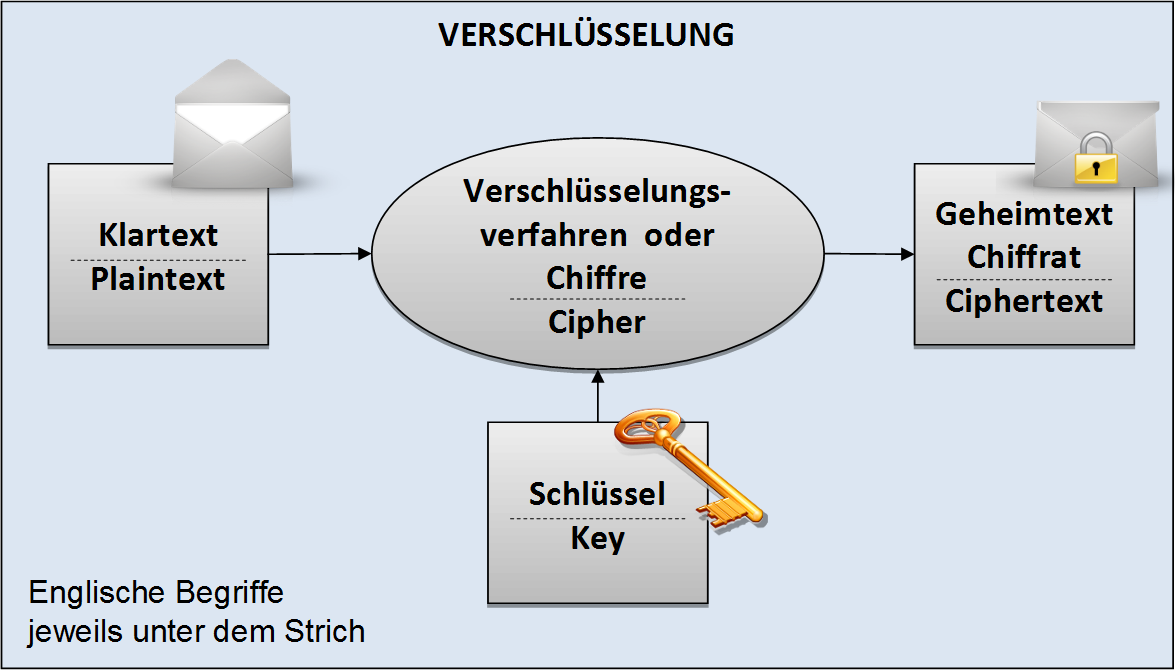
\includegraphics[scale=0.7]{figures/Generic-Notation-Encryption_de.png}
\caption{�bliche Bezeichnungen bei der Verwendung von Verschl�sselungsverfahren} 
\label{cm_Generic-Notations-when-Encrypting}
\end{center}
\end{figure}



% --------------------------------------------------------------------------
\newpage

\begin{ctsquote}
Erkl�re es mir, ich werde es vergessen.\\
Zeige es mir, ich werde es vielleicht behalten.\\
Lass es mich tun, und ich werde es k�nnen.
\caption{Indisches Sprichwort}
\end{ctsquote}


% --------------------------------------------------------------------------
\hypertarget{cm_Section_Security_Definitions}{}
\section{Sicherheits-Definitionen und Bedeutung der Kryptologie}
\label{cm_Section_Security_Definitions}
\index{Sicherheits-Definitionen}

Zuerst erkl�ren wir, wie die Sicherheit von Kryptosystemen definiert wird.

\noindent Moderne Kryptographie basiert vor allem auf mathematischer Theorie und
Computer-Praxis. Beim Design kryptographischer Algorithmen werden Annahmen
zur Schwierigkeit von Berechnungen so gemacht, so dass sich solche Verfahren
in der Praxis von einem Angreifer nur schwer brechen lassen.

\vskip +3pt
Die zwei Hauptnotationen in der Literatur definieren Sicherheit in
Abh�ngigkeit von den M�glichkeiten des Angreifers (vgl. z.B.
{\em Contemporary Cryptography} \cite{Oppliger2011}):

\begin{itemize}

\item {\bf Berechenbare, bedingte oder praktische Sicherheit}\\
  Ein Verschl�sselungsverfahren ist {\em berechenbar} sicher, wenn es (obwohl
  es theoretisch m�glich ist, es zu brechen) selbst mit den besten bekannten
  Verfahren nicht gebrochen werden kann. Theoretische Fortschritte (z.B.
  Verbesserungen bei den Algorithmen zur Faktorisierung) und schnellere
  Computer erfordern, dass dies st�ndig angepasst wird. 

  Selbst wenn man den besten bekannten Algorithmus zum Brechen benutzt, wird
  man so viele Ressourcen brauchen (z.B. 1.000.000 Jahre), dass das Kryptosystem
  sicher ist.

  Daher basiert dieses Konzept auf Annahmen �ber die begrenzte Rechenkraft des
  Angreifers und auf dem aktuellen Stand der Wissenschaft.

\item {\bf Informations-theoretische oder unbedingte Sicherheit}\\
  Ein Verschl�sselungsverfahren wird als {\em unbedingt} sicher bezeichnet,
  wenn seine Sicherheit gew�hrleistet ist, v�llig unabh�ngig davon, wieviele
  Ressourcen (Zeit, Speicher) der Angreifer hat -- also auch in dem Fall,
  wenn der Angreifer unbegrenzt viele Ressourcen hat, um das
  Verfahren zu brechen. Auch mit unbegrenzt vielen Ressourcen kann der
  Angreifer aus dem Chiffrat keine sinnvollen Informationen gewinnen.

  Es gibt Informations-theoretisch sichere Verfahren, die beweisbar nicht
  gebrochen werden k�nnen, auch nicht mit unendlich viel Rechenkraft -- ein
  Beispiel daf�r ist das {\em One-Time-Pad} (OTP\index{OTP}).

  Da das OTP ein Informations-theoretisch sicheres Verschl�sselungsverfahren
  ist, leitet sich seine Sicherheit schon allein aus der Informationstheorie
  ab -- und ist sicher, auch wenn der Angreifer unbegrenzte Rechenkapazit�ten
  hat. Das OTP weist allerdings einige praktische Nachteile auf (der
  verwendete Schl�ssel darf nur einmal verwendet werden, muss zuf�llig
  gew�hlt werden und mindestens so lang sein wie die zu sch�tzende Nachricht),
  so dass es au�er in geschlossenen Umgebungen, zum Beispiel beim hei�en
  Draht zwischen Moskau und Washington, kaum eine Rolle spielt.%\par \vskip + 3pt

\end{itemize}


\vskip +3pt
\noindent Manchmal werden auch zwei weitere Konzepte verwendet:

\begin{itemize}

\item {\bf Beweisbare Sicherheit}
Dies bedeutet, dass das Brechen eines Kryptosystems mindestens so schwierig ist
wie die L�sung eines bestimmten schwierigen Problems, z.B. die Berechnung des
diskreten Logarithmus, die diskrete Quadratwurzel-Berechnung oder die
Faktorisierung sehr gro�er Zahlen.

Beispiel: Aktuell wissen wir, dass RSA\index{RSA} h�chstens so schwierig
ist wie die Faktorisierung, aber wir k�nnen nicht beweisen, dass es genauso
schwierig ist.
Deshalb hat RSA keine beweisbare Mindest-Sicherheit. Oder in anderen Worten:
Wir k�nnen nicht beweisen, dass wenn das Kryptosystem RSA gebrochen ist, dass
dann auch die Faktorisierung (ein schwieriges mathematisches Problem) gel�st
werden kann.

Das Rabin-Kryptosystem war das erste Kryptosystem, f�r das sich beweisen lie�,
dass es berechenbar �quivalent zu einem harten mathematischen Problem ist.

\item {\bf Ad-hoc-Sicherheit}
Ein kryptographisches System hat diese Sicherheit, wenn es sich nicht lohnt,
es zu versuchen es zu brechen, weil der Aufwand daf�r teurer ist als der Wert
der Daten, die man durch das Brechen erhalten w�rde. Z.B. weil ein Angriff
nicht in einer ausreichend kurzen Zeit erfolgen kann (vgl.
{\em Handbook of Applied Cryptography} \cite{Menezes2001}).

Dies kann z.B. zutreffen, wenn B�rsen-relevante Daten sowieso am
n�chsten Tag ver�ffent"-licht werden und man f�r das Brechen ein Jahr brauchen
w�rde.

\end{itemize}


\vskip +3pt
Bei den heutzutage verwendeten guten Verfahren ist der Zeitaufwand zum Brechen
so hoch, dass sie praktisch nicht gebrochen werden k�nnen. Deshalb kann man
diese Verfahren als (praktisch) sicher ansehen -- aus einer rein auf den
Algorithmus bezogenen Sichtweise.\footnote{%
  Insbesondere seit den Informationen von Edward Snowden\index{Snowden, Edward} gab es
  viele Diskussionen, ob Verschl�sselung sicher ist. In \cite{Esslinger2014} wird das
  Ergebnis einer Evaluierung vorgestellt, auf welche Kryptographie man sich verlassen
  kann -- nach dem heutigen Kenntnisstand.
  Der Artikel untersucht: Welche Krypto-Verfahren k�nnen im Lichte der NSA-Enth�llungen
  noch als sicher gelten? Wo wurden Systeme gezielt geschw�cht? Wie k�nnen wir die
  kryptographische Zukunft sicher gestalten? Wie unterscheiden sich Mathematik und
  Implementierung?
}

\vskip +3pt
\begin{sloppypar}
Grunds�tz"-lich unterscheidet man zwischen symmetrischen
(siehe Kapitel \ref{cm_Section_Symmetric-encryption}) und asymmetrischen
(siehe Kapitel \ref{cm_Section_Asymmetric-encryption})
Verfahren zur Verschl�sse"-lung.
Einen sehr guten �berblick �ber die verschiedenen Verschl�sselungsverfahren
bieten auch die B�cher von Bruce Schneier \cite{Schneier1996} und Klaus Schmeh
\cite{Schm2016}.\footnote{%
  Einen kompakten �berblick, der erkl�rt, was wozu verwendet wird, welche der Verfahren
  sicher sind, wo mit Problemen zu rechnen ist und wo die wichtigen Baustellen f�r die
  absehbare Zukunft liegen incl. des Procederes bei den Standardisierungen finden Sie
  in \cite{Schmidt2016}.
  % TODO Info an ju, dass Schreibweise korr ("s" anh�ngen)
  %%     bei "Bereits 1883 formulierte Auguste Kerckhoff".
  % Dieser Artikel erschien urspr�nglich in c't 01/2016, Seite 174
  % Kryptographie in der IT - Empfehlungen zu Verschl�sselung und Verfahren.
  % Kryptographie ist ein wichtiger Baustein moderner IT � Sicherheit,
  % Vertraulichkeit und Privatsph�re h�ngen davon ab. Der folgende Krypto-Wegweiser
  % gibt einen kompakten �berblick zu den aktuell relevanten Verfahren.
}
\end{sloppypar}

\vskip +3pt
Bevor Verschl�sselungstechnologien mit dem Aufkommen des Internets und der drahtlosen
Kommunikation f�r jedermann zur Verf�gung standen, waren sie schon seit Jahrhunderten
im Gebrauch von Regierungen, Milit�rs und Diplomaten. Welche Seite diese Technologie
besser beherrschte konnte mit Hilfen der Geheimdienste gro�en Einfluss auf die {\bf Politik}
und den Kriegsverlauf nehmen. Auf die Historie geht dieses Buch nur insofern ein, als
in Kapitel \ref{Chapter_PaperandPencil} auch die fr�her benutzten Verfahren vorgestellt
werden. Einen Eindruck, welch entscheidende Bedeutung Kryptologie f�r die M�chtigen
hatte und hat, kann man anhand der beiden folgenden Beispiele bekommen: dem Lehrfilm
\glqq Krieg der Buchstaben\grqq\footnote{%
  Der Film \index{Krieg der Buchstaben} schildert vor dem Hintergrund der Weltpolitik
  von 1900-1945 die Entwicklung der Kryptologie und ihre Bedeutung f�r den
  Kriegsverlauf im ersten (Zimmermann-Depesche) und zweiten Weltkrieg. Ausf�hrlich
  wird -- aus anglo-amerikanischer Sicht -- darauf eingegangen, wie bedeutsam die
  Kryptoanalyse (auf dem Atlantik gegen die Enigma und auf dem Pazifik gegen Purple)
  f�r den Verlauf des zweiten Weltkriegs war.\\
  Siehe \url{http://bscw.schule.de/pub/bscw.cgi/d1269787/Krieg_der_Buchstaben.pdf}.
}
und der Debatte um die sogenannten Krypto-Wars\footnote{%
  Siehe \url{https://de.wikipedia.org/wiki/Crypto_Wars}.\index{Krypto-Wars}
}.
%% Vgl. http://scilogs.spektrum.de/hlf/verschluesselte-hintertuerchen-tag-internet-licht/
%%      http://www.heidelberg-laureate-forum.org/de/2015/08/17/eine-debatte-ueber-die-herausforderungen-einer-datengesteuerten-welt/
%%      http://wwwde.uni.lu/snt/news_events/prof_peter_ryan_gives_lecture_at_heidelberg_laureate_forum
%% Diskussion auf dem 3. Heidelberg Laureate Forum (HLF) am Dienstag, 25. August 2015.


% --------------------------------------------------------------------------
\newpage

\begin{ctsquote}
\glqq Man kann nicht nicht kommunizieren!\grqq 
\caption[Paul Watzlawick]{Paul Watzlawick\footnotemark}\index{Watzlawick, Paul}
\end{ctsquote}
\addtocounter{footnote}{0}\footnotetext{Paul Watzlawick, Janet H. Beavin und Don D. Jackson, \glqq Menschliche Kommunikation. Formen, St�rungen, Paradoxien\grqq, Huber, (c) 2007, Das erste der f�nf pragmatischen Axiome ihrer Kommunikationstheorie.}

% --------------------------------------------------------------------------
\section[Einfl�sse auf Verschl�sselungsverfahren] % Was zw. [..] steht, kommt ins Inhaltsverzeichnis!
{Einfl�sse auf Verschl�sselungsverfahren}

% \nopagebreak
Hier sollen kurz zwei Aspekte von Kryptoverfahren erw�hnt werden, auf die oft nicht fr�h genug eingegangen wird:

\begin{itemize}

\item {\bf Zufallsbasiert}\\
\index{Zufall}
Man kann Algorithmen aufteilen in deterministische\index{deterministisch} und heuristische\index{heuristisch} Verfahren. Meistens lernten Studenten nur deterministische Verfahren kennen, bei denen die Ausgabe eindeutig durch die Eingabe vorgegeben wird. Bei heuristischen Verfahren werden Entscheidungen aufgrund zuf�lliger Werte getroffen. Moderne Verfahren des maschinellen Lernens geh�ren ebenfalls hierzu.

In Kryptoverfahren spielt Zufall eine gro�e Rolle. Immer m�ssen die Schl�ssel zuf�llig gew�hlt werden, so dass zumindest bei der Schl�sselgenerierung~\glqq Zufall\grqq~erzeugt werden muss. Zus�tzlich sind manche Verfahren (vor allem aus der Kryptoanalyse) heuristisch.

\item {\bf Konstanten-basiert}\\
Viele moderne Verfahren (insbesondere Hashverfahren und symmetrische Verschl�sse-lungsverfahren) benutzen numerische Konstanten. Diese sollten nachvollziehbar sein und keine Hintert�ren erm�glichen. Zahlen, die das erf�llen, nennt man im Englischen~\glqq Nichts-im-�rmel\grqq-Zahlen: Nothing-up-my-sleeve number\index{Zahlen!Nothing-up-my-sleeve}.%
\footnote{\url{http://en.wikipedia.org/wiki/Nothing_up_my_sleeve_number}}

\end{itemize}


\newpage
Die folgende Abbildung \ref{cm_Figure_OTP-demo-pictures} soll eine Idee davon vermitteln, dass es nicht m�glich ist, bei einem OTP\index{OTP} den Klartext zu bestimmen (sofern das OTP-Verfahren richtig angewendet wird und alle Schl�ssel gleich wahrscheinlich sind).

In dem Beispiel in der Abbildung ist als Geheimtext ein 8 Zeichen langes Wort gegeben:
\texttt{11 1B 1E 18 00 04 0A 15}.
Es gibt viele sinnvolle Worte aus 8 Buchstaben und zu jedem einen passenden Schl�ssel.
Ein Angreifer kann damit allein nicht bestimmen, welches der richtige Schl�ssel bzw.
welches das richtige Klartext-Wort ist.

Vergleiche auch Abbildung~\ref{fig-bool-otp} in Kapitel \ref{s-bool-bitstr-real-random},
wo ein entsprechendes Text-Beispiel mit SageMath erstellt wird.
\begin{figure}[ht]
\begin{center}
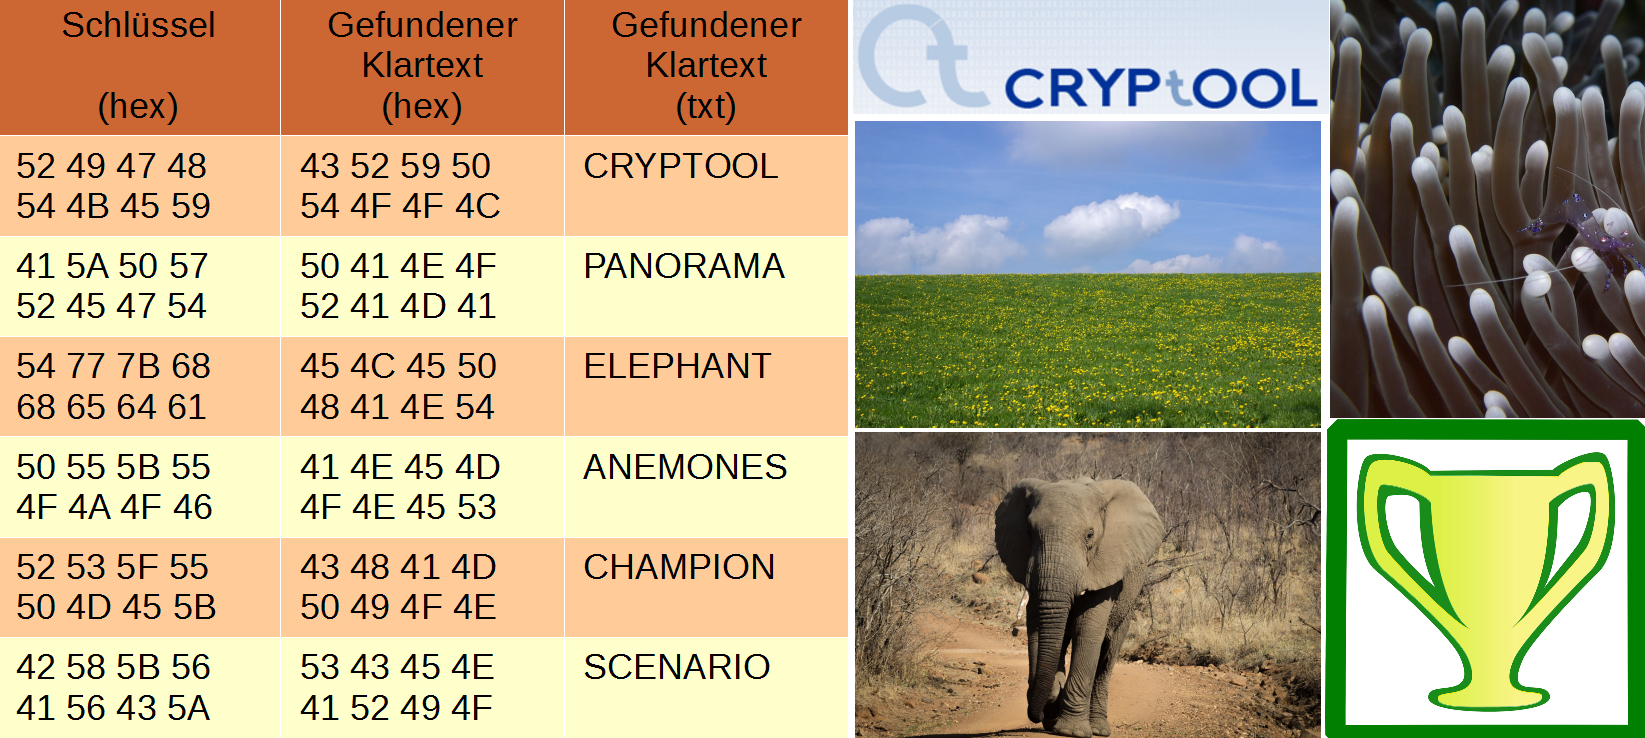
\includegraphics[scale=0.55]{figures/OTP-demo-pictures-de.png}
\caption[Illustration f�r die Informations-theoretische Sicherheit des OTP]
        {Illustration f�r die Informations-theoretische Sicherheit des OTP\footnotemark}
\label{cm_Figure_OTP-demo-pictures}
\end{center}
\end{figure}
\footnotetext{
  Bildquelle: Kostenlose Bilder von \url{https://pixabay.com/}
}





% --------------------------------------------------------------------------
\newpage

\begin{ctsquote}
\glqq Transparenz. Das ist das H�chste, was man sich in einer technologisch hoch entwickelten Gesellschaft erhoffen kann ... sonst wird man einfach nur manipuliert.\grqq 
\caption[Daniel Suarez]{Daniel Suarez\footnotemark}\index{Suarez, Daniel}
\end{ctsquote}
\addtocounter{footnote}{0}\footnotetext{Daniel Suarez, \glqq Darknet\grqq,
            rororo, (c) 2011, Kapitel 5, \glqq Einsichten\grqq, S. 69, Price.}

% --------------------------------------------------------------------------
\section[Symmetrische Verschl�sselung] % Was zwischen [...] steht, kommt ins Inhaltsverzeichnis!
        {Symmetrische Verschl�sselung\footnotemark}
  \footnotetext{% Dieses Prozent ist n�tig, sonst startet die Fu�note mit einem Blank !
    Mit CrypTool~1 ({\bf CT1})\index{CT1} k�nnen Sie �ber das
    Men� {\bf Ver-/Entschl�sseln \textbackslash{} Symmetrisch (modern)} folgende
    modernen symmetrischen Verschl�sselungsverfahren ausf�hren:\\
    IDEA, RC2, RC4, DES (ECB), DES (CBC), Triple-DES (ECB), Triple-DES (CBC),
    MARS (AES-Kandidat), RC6 (AES-Kandidat), Serpent (AES-Kandidat), 
    Twofish (AES-Kandidat),
    Rijndael (offizielles AES-Verfahren)\index{AES}.\\
    Mit CrypTool~2 ({\bf CT2})\index{CT2} k�nnen Sie im Startcenter
    �ber {\bf Vorlagen \textbackslash{} Kryptographie \textbackslash{}
    Modern \textbackslash{} Symmetrisch} folgende modernen symmetrischen
    Verschl�sselungsverfahren ausf�hren:\\ 
    AES, DES, PRESENT, RC2, RC4, SDES, TEA, Triple-DES, Twofish.\\
    In JCrypTool ({\bf JCT})\index{JCT} stehen Ihnen die folgenden
    modernen symmetrischen Verschl�sselungsverfahren zur Verf�gung:\\ 
    AES, Rijndael, Camellia, DES, Dragon, IDEA, LFSR, MARS, Misty1, RC2, RC5,
    RC6, SAFER+, SAFER++, Serpent, Shacal, Shacal2, Twofish.
    }
\label{cm_Section_Symmetric-encryption}

\nopagebreak

Bei der {\em symmetrischen} Verschl�sselung 
\index{Verschl�sselung!symmetrisch} m�ssen Sender und Empf�nger
�ber einen gemeinsamen (geheimen) Schl�ssel verf�gen, den sie vor
Beginn der eigentlichen Kommunikation ausgetauscht haben. Der Sender
benutzt diesen Schl�ssel, um die Nachricht zu verschl�sseln und der
Empf�nger, um diese zu entschl�sseln.\par %\vskip + 3pt

Dies veranschaulicht Abbildung \ref{cm_Figure_Symmetric-Enc_Secret-Key-Enc}:
\begin{figure}[ht]
\begin{center}
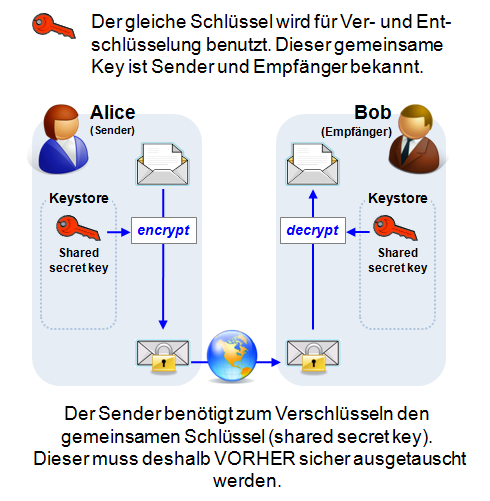
\includegraphics[scale=0.7]{figures/SymmetricEnc_Figure_Chap1_de.png}
\caption{Symmetrische oder Secret-Key-Verschl�sselung} 
\label{cm_Figure_Symmetric-Enc_Secret-Key-Enc}
\end{center}
\end{figure}

Alle klassischen Chiffren sind vom Typ symmetrisch. Beispiele dazu finden Sie
in den CT-Programmen, im Kapitel~\ref{Chapter_PaperandPencil}
(\glqq \nameref{Chapter_PaperandPencil}\grqq)
in diesem Skript oder in \cite{Nichols1996}. 
In diesem Unterkapitel wollen wir jedoch nur die moderneren symmetrischen
Verfahren betrachten.

Vorteile von symmetrischen Algorithmen sind die hohe
Geschwindigkeit, mit denen Daten ver- und entschl�sselt werden.
Ein Nachteil ist das Schl�sselmanagement. Um miteinander
vertraulich kommunizieren zu k�nnen, m�ssen Sender und
Empf�nger vor Beginn der eigentlichen Kommunikation �ber einen
sicheren Kanal einen Schl�ssel ausgetauscht haben. Spontane
Kommunikation zwischen Personen, die sich vorher noch nie begegnet
sind, scheint so nahezu unm�glich. Soll in einem Netz mit $ n $
Teilnehmern jeder mit jedem zu jeder Zeit spontan kommunizieren
k�nnen, so muss jeder Teilnehmer vorher mit jedem anderen der
$n - 1$ Teilnehmer einen Schl�ssel ausgetauscht haben. Insgesamt
m�ssen also $n(n - 1)/2$ Schl�ssel ausgetauscht werden.\par \vskip + 3pt



\subsection[AES (Advanced Encryption Standard)]{AES (Advanced Encryption Standard)\footnotemark} 
\footnotetext{%
   In CT1\index{CT1} finden Sie 3 Visualisierungen dieses Verfahrens
   �ber das Men� {\bf Einzelverfahren \textbackslash{} Visualisierung von
   Algorithmen \textbackslash{} AES}.\\
   In CT2\index{CT2} k�nnen Sie im Startcenter
   mit dem Suchstring \glqq AES\grqq~eine Vorlage (Template) finden,
   die den Algorithmus Schritt-f�r-Schritt visualisiert.
}
\label{CM_AES}
\index{AES}

Vor AES war der DES-Algorithmus\index{DES} das bekannteste moderne, symmetrische
Verschl�sselungs"-ver"-fahren. Der DES-Algorithmus war eine Entwicklung von IBM 
in Zusammenarbeit mit der National Security Agency \index{NSA} (NSA). 
Er wurde 1975 als Standard ver�ffentlicht. Trotz seines relativ hohen
Alters ist bis heute kein~\glqq effektiver\grqq~Angriff auf
ihn gefunden worden. Der effektivste Angriff besteht aus dem Durchprobieren
(fast) aller m�glichen Schl�ssel, bis der richtige gefunden wird 
({\em Brute-Force-Angriff})\index{Angriff!Brute-Force}. Aufgrund der relativ
kurzen Schl�ssell�nge von effektiv 56 Bits (64 Bits, die allerdings 8
Parit�tsbits enthalten), sind in der Vergangenheit schon mehrfach mit dem
DES verschl�sselte Nachrichten gebrochen worden, so dass er heute nicht
mehr als sicher anzusehen ist. Alternativen zum DES sind zum Beispiel die
Algorithmen IDEA\index{IDEA}, Triple-DES (TDES) und vor allem AES.
\par \vskip + 3pt

Standard unter den symmetrischen Verfahren ist heute AES\index{AES}:
Der dazu geh�rende Rijndael-Algo"-rithmus wurde am 2. Oktober 2000 zum
Gewinner der AES-Ausschreibung erkl�rt und ist damit Nachfolger
des DES-Verfahrens.

Einen Einstieg und weitere Verweise zum AES-Algorithmus und den AES-Kandidaten
der letzten Runde finden Sie z.B. in der Online-Hilfe von
CrypTool\index{CrypTool}%
\footnote{%
      Online-Hilfe von CT1\index{CT1}: Das Stichwort {\bf AES} im Index
      f�hrt auf die drei Hilfeseiten: {\bf AES-Kandidaten}, 
      {\bf Der AES-Gewinner Rijndael} und {\bf Der AES-Algorithmus Rijndael}.\\
      Eine ausf�hrliche Beschreibung von AES mit C-Code findet sich
      in \cite{Haan2008}.
  }
oder in Wikipedia%
\footnote{%
	\url{https://de.wikipedia.org/wiki/Advanced_Encryption_Standard}
  }.


\clearpage
\noindent Die beiden Screenshots \ref{AES-Visualization-Zabala-Flash-step3} und
\ref{AES-Visualization-Zabala-Flash-step5} sind aus einer der 3
AES-Visualisierungen in CT1\index{CT1}.

% Ohne das !vor ht verteilt LaTeX die abb. auf 2 Seiten. \sloppypar hilft hier nict (nur f�r Worttrenner).
% http://texwelt.de/wissen/fragen/6667/mehrere-bilder-untereinander
\begin{figure}[!ht]
\begin{center}
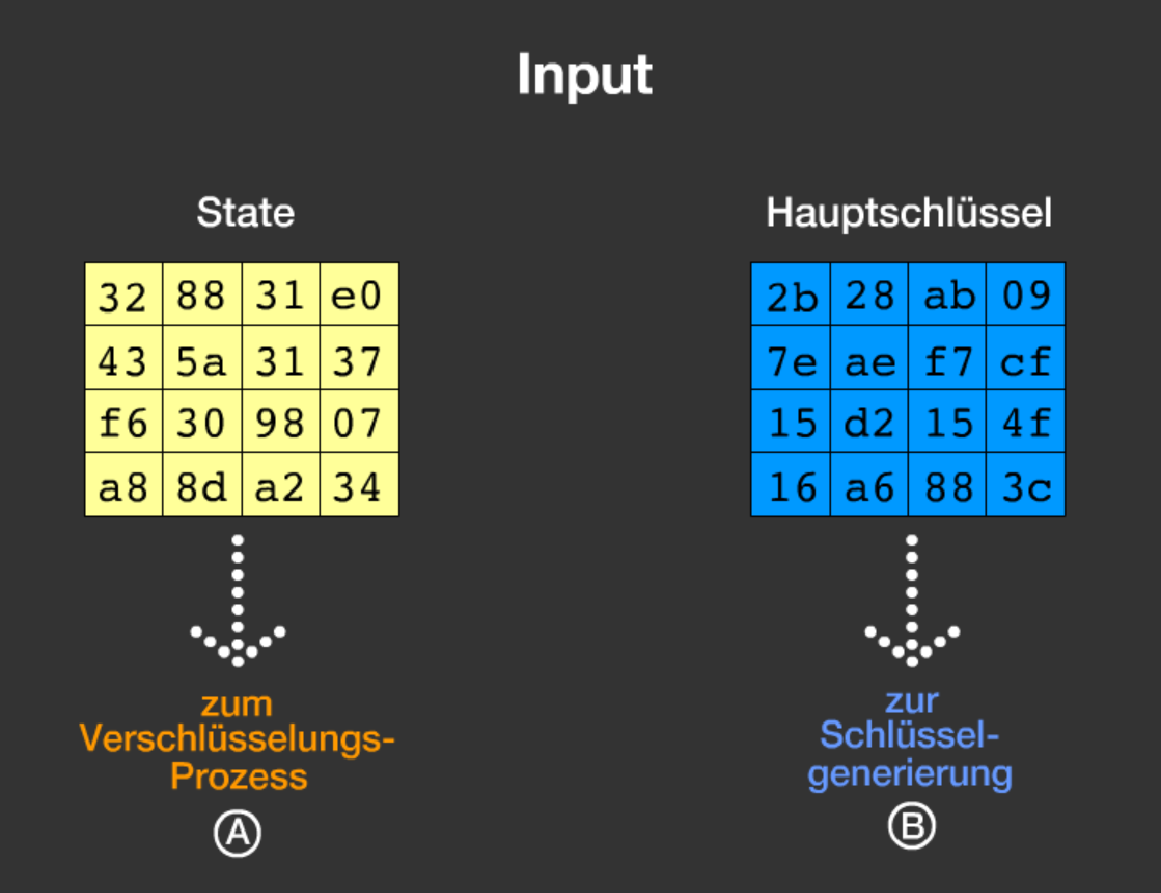
\includegraphics[scale=0.6]{figures/AES-Visualization-Zabala-Flash-step3_de}
\caption{AES-Visualisierung von Enrique Zabala aus CT1 (Teil 1)}
\label{AES-Visualization-Zabala-Flash-step3}
\end{center}
\end{figure}

\begin{figure}[!ht]
\begin{center}
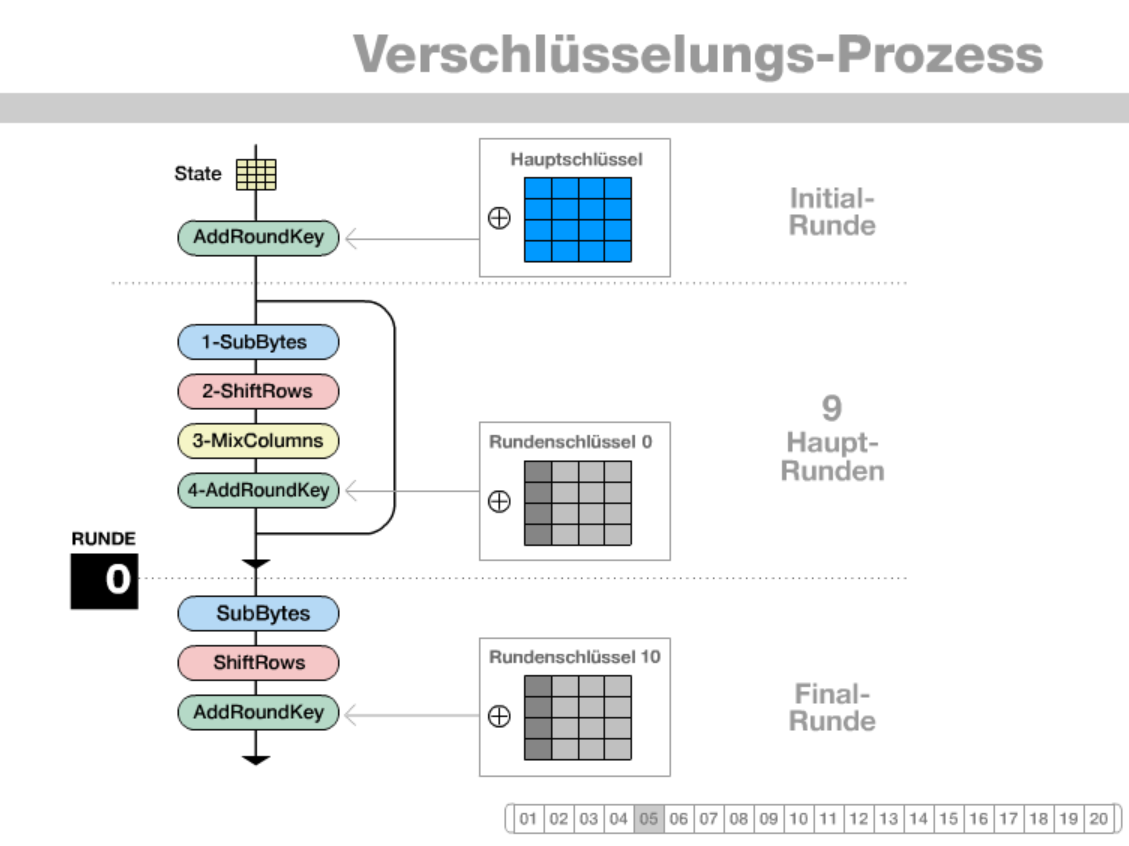
\includegraphics[scale=0.6]{figures/AES-Visualization-Zabala-Flash-step5_de}
\caption{AES-Visualisierung von Enrique Zabala aus CT1 (Teil 2)}
\label{AES-Visualization-Zabala-Flash-step5}
\end{center}
\end{figure}
%\end{sloppypar}


\clearpage
\noindent Im Folgenden wollen wir einen 128-bit-Block Klartext mit einem 128-bit
Schl�ssel mit AES im CBC-Modus verschl�sseln. Vom erhaltenen Geheimtext interessiert
uns nur der 1. Block (wenn mehr vorhanden ist, ist das Padding -- hier Null-Padding).
Zur Veranschaulichung machen wir das einmal mit CT2 und einmal mit OpenSSL.\\

\noindent Abbildung \ref{AES_Encrypting-one-block-with-CT2} zeigt die Verschl�sselung
eines Blocks in {\bf CT2}\index{CT2}.

\noindent Der Klartext \glqq AESTEST1USINGCT2\grqq~wird nach Hex
(41 45 53 54 45 53 54 31 55 53 49 4E 47 43 54 32)
konvertiert. Damit und mit dem Schl�ssel 3243F6A8885A308D313198A2E0370734
erzeugt die AES-Komponente dann den Geheimtext. Dieser lautet in Hex:\\
B1 13 D6 47 DB 75 C6 D8 47 FD 8B 92 9A 29 DE 08

\begin{figure}[ht]
\begin{center}
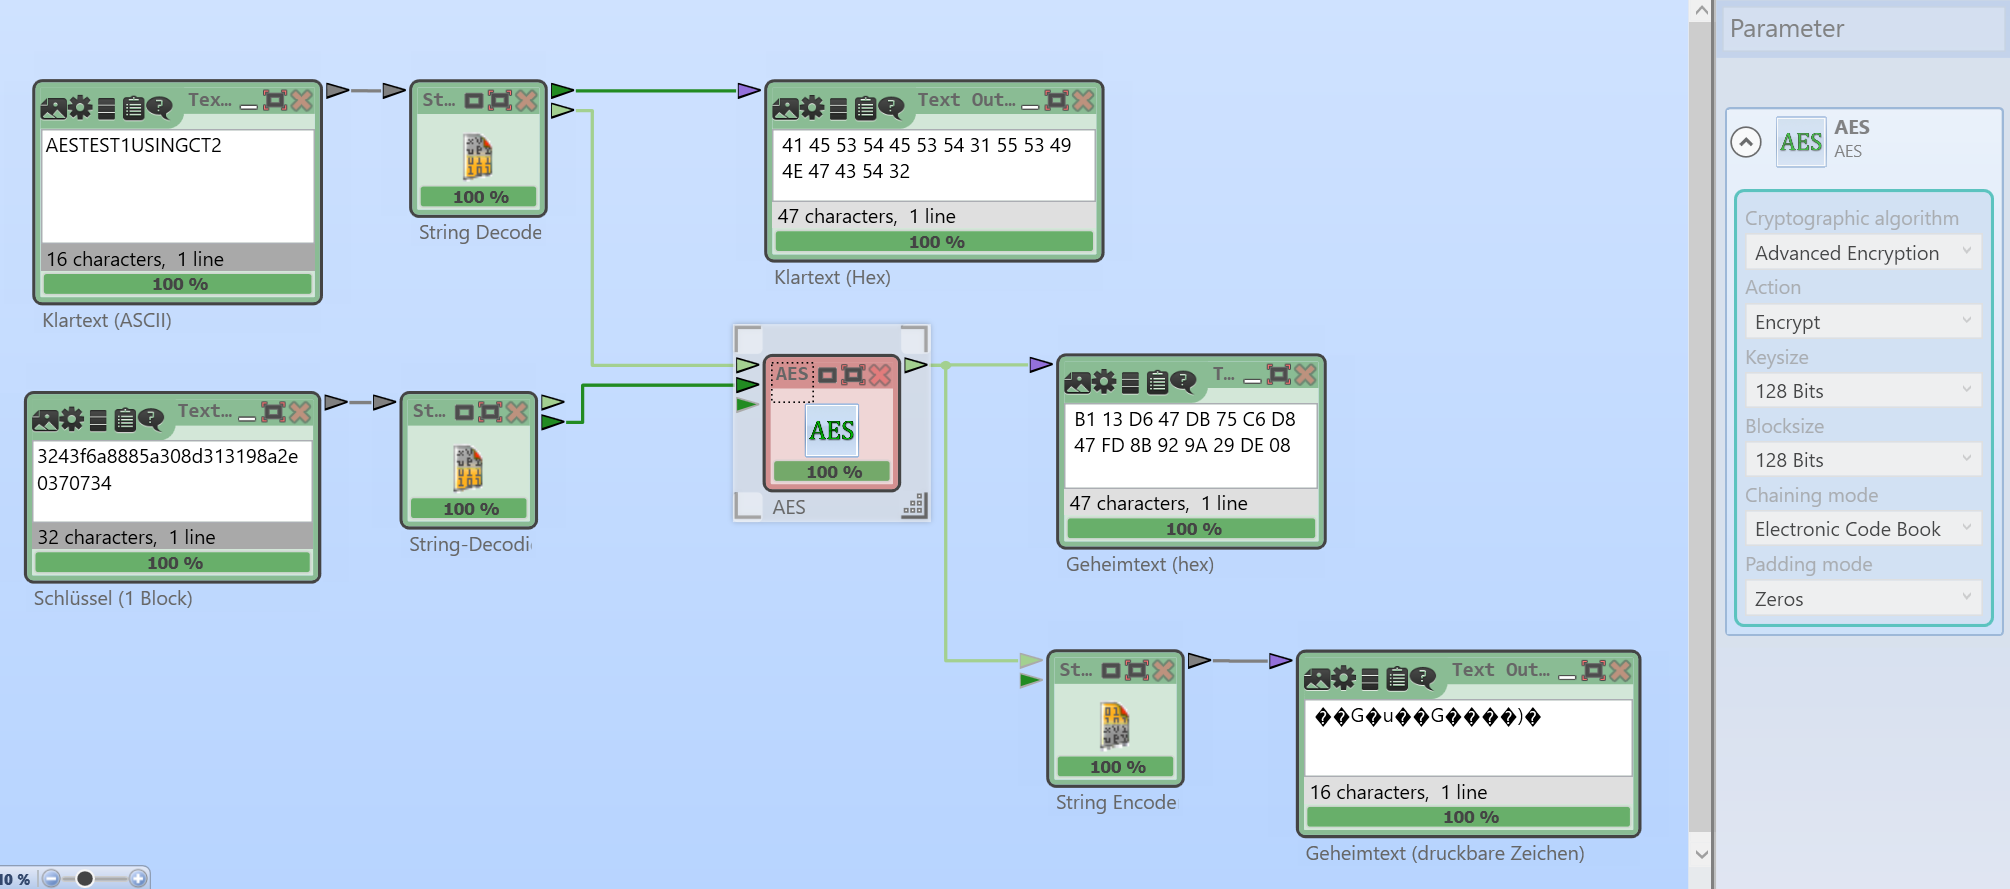
\includegraphics[scale=0.42]{figures/AES_Encrypting-one-block-with-CT2_de}
\caption{AES-Verschl�sselung (genau 1 Block ohne Padding) in CT2} 
\label{AES_Encrypting-one-block-with-CT2}
\end{center}
\end{figure}

\vspace{15pt}
\noindent Dasselbe Ergebnis kann man mit {\bf OpenSSL}\index{OpenSSL}%
\footnote{%
      OpenSSL\index{OpenSSL} ist eine sehr verbreitete freie Open-Source Kryptobibliothek,
      die von vielen Anwendungen benutzt wird, bspw. um das TLS-Protokoll zu implementieren.
      Zu OpenSSL geh�rt auch das Kommandozeilentool openssl, mit dem man die Funktionalit�t
      auf vielen Betriebssystemen direkt ausprobieren und Zertifikate beantragen, erzeugen
      und verwalten kann.\\
      Im Gegensatz zum ebenfalls sehr verbreiteten und sehr guten Kommandozeilentool gpg
      von GNU Privacy Guard\index{GnuPG}
      (\url{https://de.wikipedia.org/wiki/GNU_Privacy_Guard})
      erlaubt openssl auch Aufrufe, die sehr ins Detail gehen.
      Bei gpg liegt der Schwerpunkt auf den im praktischen Einsatz befindlichen Ciphersuites.
      Einfach genau einen Block ohne Padding zu verschl�sseln geht unseres Wissens mit dem
      Kommandozeilentool gpg nicht.\\
      Siehe auch \url{https://de.wikipedia.org/wiki/OpenSSL}.
%      Also see \url{https://en.wikipedia.org/wiki/OpenSSL}.
  }
auf der Kommandozeile auf ff. Weise erzielen:
\begin{opensslcode}
\begin{Verbatim}%
[fontsize=\footnotesize]
>openssl enc -e -aes-128-cbc
        -K 3243F6A8885A308D313198A2E0370734
        -iv 00000000000000000000000000000000
        -in klartext-1.hex  -out klartext-1.hex.enc
>dir
06.07.2016  12:43                16 key.hex
20.07.2016  20:19                16 klartext-1.hex
20.07.2016  20:37                32 klartext-1.hex.enc
\end{Verbatim}
\caption{AES-Verschl�sselung (von genau einem Block ohne Padding) in OpenSSL}
\label{cm_AES_no-padding:OpenSSL_example}
\end{opensslcode}





\clearpage
% HACK to fix warning "destination with the same identifier .. has already been used, ...":
% REMOVED, because it caused missing index entries
%\makeatletter \renewcommand{\thepage}{\csname @arabic\endcsname \c@page} \makeatother
% --------------------------------------------------------------------------
\subsubsection{Ergebnisse zur theoretischen Kryptoanalyse von AES}
\label{cm_New-AES-Analysis}
\index{Kryptoanalyse}
\index{AES}

Im Anschluss finden Sie einige Informationen, die das AES-Verfahren in
letzter Zeit in Zweifel zogen -- unserer Ansicht nach aber (noch)
unbegr�ndet. Die folgenden Informationen beruhen vor allem auf den unten
angegebenen Originalarbeiten und auf \cite{Wobst2002} und
\cite{Lucks2002}.

Der AES bietet mit einer Mindestschl�ssell�nge von 128 Bit gegen
Brute-Force-Angriffe auch auf l�ngere Sicht gen�gend Sicherheit -- es sei
denn, es st�nden entsprechend leistungsf�hige Quantencomputer zur
Verf�gung. Der AES war immun gegen alle bis dahin bekannten
Krypto"-analyse-Verfahren, die vor allem auf statistischen
�berlegungen beruhen und auf DES angewandt wurden: man konstruiert aus
Geheim- und Klartextpaaren Ausdr�cke, die sich nicht rein zuf�llig
verhalten, sondern R�ckschl�sse auf den verwendeten Schl�ssel zulassen.
Dazu waren aber unrealistische Mengen an abgeh�rten Daten n�tig.

Bei Kryptoverfahren bezeichnet man solche Kryptoanalyseverfahren als
"`akademischen Erfolg"' oder als "`kryptoanalytischen Angriff"', da sie
theoretisch schneller sind als das Durchprobieren aller Schl�ssel, das
beim Brute-Force-Angriff\index{Angriff!Brute-Force} verwendet wird. Im
Fall des AES mit maximaler Schl�ssell�nge (256 Bit) braucht die
ersch�pfende Schl�sselsuche im Durchschnitt $2^{255}$
Verschl�sselungsoperationen. Ein kryptoanalytischer Angriff muss diesen
Wert unterbieten. Als aktuell gerade noch praktikabel (z.B. f�r einen
Geheimdienst) gilt ein Aufwand von $2^{75}$ bis $2^{90}$
Verschl�sselungsoperationen.

Eine neue Vorgehensweise wurde in der Arbeit von Ferguson, Schroeppel
und Whiting im Jahre 2001 \cite{Ferguson2001} beschrieben: Sie stellten
AES als geschlossene Formel (in der Form einer Art Kettenbruch) dar,
was aufgrund seiner "`relativ"' �bersichtlichen Struktur gelang. Da
diese Formel aus rund 1 Billiarde Summanden besteht, taugt sie zun�chst
nicht f�r die Kryptoanalyse. Dennoch war die wissenschaftliche Neugier
geweckt. Bereits bekannt war, dass sich der 128-Bit-AES als ein
�berbestimmtes System von rund 8000 quadratischen Gleichungen
(�ber algebraischen Zahlk�rpern) mit rund 1600 Variablen (einige
Unbekannte sind die Schl�sselbits) darstellen l�sst -- solch gro�e
Gleichungssysteme sind praktisch nicht l�sbar. Dieses Gleichungssystem
ist relativ d�nn besetzt (\glqq sparse\grqq), d.h. von den insgesamt etwa
1.280.000 m�glichen quadratischen Termen tauchen nur relativ wenige
�berhaupt im Gleichungssystem auf.

Die Mathematiker Courtois und Pieprzyk \cite{Courtois2002} ver�ffentlichten 
2002 eine Arbeit, die in der Krypto-Szene stark diskutiert wird: Sie 
entwickelten das auf der Eurocrypt 2000 von Shamir et al. vorgestellte 
XL-Verfahren (eXtended Linearization) weiter zum XSL-Verfahren 
(eXtended Sparse Linearization). Das XL-Verfahren ist eine heuristische 
Technik, mit der es manchmal gelingt, gro�e nicht-lineare Gleichungssysteme 
zu l�sen und die bei der Analyse eines asymmetrischen Algorithmus (HFE) 
angewandt wurde.  Die Innovation von Courtois und Pieprzyk war, das 
XL-Verfahren auf symmetrische Verfahren anzuwenden: Das XSL-Verfahren kann
auf spezielle Gleichungssysteme angewandt werden. Damit k�nnte ein 
256-Bit-AES-Verfah"-ren in rund $2^{230}$ Schritten geknackt werden. Dies ist 
zwar immer noch ein rein akademischer Angriff, aber er ist richtungsweisend
f�r eine ganze Klasse von Blockchiffren. Das generelle Problem mit diesem
Angriff besteht darin, dass man bisher nicht angeben kann, unter welchen
Umst�nden er zum Erfolg f�hrt: die Autoren geben in ihrer Arbeit notwendige
Bedingungen an; es ist nicht bekannt, welche Bedingungen hinreichend sind.
Neu an diesem Angriff war erstens, dass dieser Angriff nicht auf Statistik,
sondern auf Algebra beruhte. Dadurch erscheinen Angriffe m�glich, die nur
geringe Mengen von Geheimtext brauchen. Zweitens steigt damit die Sicherheit
eines Produktalgorithmus%
\index{Produktalgorithmus}\index{Verschl�sselung!Produktalgorithmus}%
\footnote{%
Ein Geheimtext kann selbst wieder Eingabe f�r eine Chiffrierung sein. Eine
Mehrfachverschl�sselung (cascade cipher)
\index{Verschl�sselung!Mehrfachverschl�sselung}\index{Mehrfachverschl�sselung}
\index{Kaskaden}
entsteht aus einer Komposition von mehreren Verschl�sselungstransformationen.
Die Gesamtchiffrierung wird Produktalgorithmus oder Kaskadenalgorithmus
genannt (manchmal ist die Namensgebung abh�ngig davon, ob die verwendeten
Schl�ssel statistisch abh�ngig oder unabh�ngig sind).\\
Nicht immer wird die Sicherheit eines Verfahrens durch Produktbildung 
erh�ht.\\
Dieses Vorgehen wird auch {\em innerhalb} moderner Algorithmen angewandt:
Sie kombinieren in der Regel einfache und, f�r sich genommen, kryptologisch
relativ unsichere Einzelschritte in mehreren Runden zu einem leistungsf�higen
Gesamtverfahren. Die meisten modernen Blockchiffrierungen (z.B. DES, IDEA)
sind Produktalgorithmen.\\
Als Mehrfachverschl�sselung wird auch das Hintereinanderschalten desselben
Verfahrens mit verschiedenen Schl�sseln wie bei Triple-DES bezeichnet.\index{DES!Triple-DES}
}
nicht mehr exponentiell mit der Rundenzahl.

Aktuell wird sehr intensiv auf diesem Gebiet geforscht: z.B. stellten
Murphy und Robshaw auf der Crypto 2002 ein Papier vor \cite{Robshaw2002a},
das die Kryptoanalyse drastisch verbessern k�nnte: Der Aufwand f�r
128-Bit-Schl�ssel wurde auf $2^{100}$ gesch�tzt, indem sie AES als
Spezialfall eines Algorithmus BES (Big Encryption System) darstellten,
der eine besonders "`runde"' Struktur hat. Aber auch $2^{100}$
Rechenschritte liegen jenseits dessen, was praktisch in absehbarer Zeit
realisierbar ist. Bei 256 Bit Schl�ssell�nge sch�tzen die Autoren
den Aufwand f�r den XSL-Angriff auf $2^{200}$ Operationen.

Weitere Details finden Sie unter den Weblinks bei
\hyperlink{CM_HT_Weblink_Rijndael-Cryptosystem}{\glqq Das AES-/Rijndael-Kryptosystem\grqq}.
% nur \href oder \url r�ckt nicht ein, deshalb \item dazu !
%\vspace{-10pt}
%\begin{itemize}
%  \item[] \url{http://www.cryptosystem.net/aes} \\
%          \url{http://www.minrank.org/aes/} 
%\end{itemize}


F�r AES-256 w�re der Angriff ebenfalls viel besser als
Brute-Force\index{Angriff!Brute-Force}, aber noch weit au�erhalb der
Reichweite realisierbarer Rechenpower.

\begin{sloppypar}
Die Diskussion ist z.Zt. sehr kontrovers: Don Coppersmith (einer der
DES-Erfinder) z.B. bezweifelt die generelle Durchf�hrbarkeit des Angriffs:
XLS liefere f�r AES gar keine L�sung \cite{Coppersmith2002}. Dann w�rde
auch die Optimierung von Murphy und Robshaw \cite{Robshaw2002b} nicht
greifen.
\end{sloppypar}

2009 ver�ffentlichten Biryukov und Khovratovich \cite{Biryukov2009} einen
weiteren theoretischen Angriff auf AES, der sich anderer Techniken bedient, als
die oben vorgestellten. Sie verwenden Methoden aus der Kryptoanalyse von
Hashfunktionen (lokale Kollisionen und das Boomerang-Verfahren) und
konstruierten daraus einen Related-Key-Angriff auf AES-256. D.~h.\ der Angreifer
muss nicht nur in der Lage sein, beliebige Daten zu verschl�sseln (chosen plain
text), sondern auch den ihm unbekannten Schl�ssel manipulieren k�nnen (related
key).

Unter diesen Angriffs-Voraussetzungen reduziert der Angriff den Aufwand, einen
AES-256-Schl�ssel zu ermitteln, auf eine (asymmetrische) Komplexit�t von
$2^{119}$ Zeit und $2^{77}$ Speicher. Bei AES-192 ist der Angriff noch weniger
praktikabel, f�r AES-128 geben die Autoren keinen Angriff an.


% --------------------------------------------------------------------------
\subsection{Algebraische oder algorithmische Kryptoanalyse symmetrischer Verfahren}
\index{Angriff!algebraisch}
\label{cm_Algebraic-versus-Symmetr}

Es gibt unterschiedliche moderne Angriffsverfahren, die die Strukturen eines Problems direkt oder nach einer Transformation des Problems angreifen. Eines dieser Angriffsverfahren beruht auf dem Erf�llbarkeitsproblem der Aussagenlogik (SAT, von englisch satisfiability)%
\footnote{%
 \url{http://de.wikipedia.org/wiki/Erf%C3%BCllbarkeitsproblem_der_Aussagenlogik}
}.


%\vskip +25 pt
\paragraph*{Beschreibung SAT-Solver}\index{SAT-Solver}\mbox{}
\hypertarget{ht_SAT-Solver}{}

Ein sehr altes und gut studiertes Problem in der Informatik ist das sogenannte SAT-Problem. Hier gilt es, f�r eine gegebene Boolesche Formel herauszufinden, ob es eine Belegung der Variablen gibt, so dass die Auswertung der Formel den Wert 1 ergibt. 

Beispiel: Die Formel \glqq A UND B\grqq~wird zu 1 ausgewertet, wenn A=B=1 gilt. F�r die Formel \glqq A UND NICHT(A)\grqq~gibt es keine Belegung f�r A, so dass sie zu 1 ausgewertet wird.

F�r gr��ere Formeln ist es nicht so einfach herauszufinden, ob eine Formel zu 1 ausgewertet werden kann (dieses Problem geh�rt zu den NP-vollst�ndigen Problemen). Daher wurden spezielle Tools entwickelt, um dieses Problem f�r generelle Boolesche Formeln zu l�sen, sogenannte SAT-Solver\footnote{
    Mit {\bf CT2}\index{CT2} k�nnen Sie im Startcenter
    �ber {\bf Vorlagen \textbackslash{} Mathematisch \textbackslash{}
    SAT-Solver (Texteingabe)}  und  {\bf SAT-Solver (Dateieingabe)} einen
    SAT-Solver aufrufen.
    }. Wie sich herausgestellt hat, k�nnen SAT-Solver auch eingesetzt werden, um Krypto-Verfahren
anzugreifen.


%\vskip +25 pt
\paragraph*{SAT-Solver basierte Kryptoanalyse}\index{SAT-Solver}\mbox{}
\hypertarget{ht_SAT-Solver_Cryptanalysis}{}

Der generelle Ansatz, um SAT-Solver in der Kryptoanalyse einzusetzen, ist sehr einfach: Zun�chst wird das kryptographische Problem, etwa das Finden des symmetrischen Schl�ssels oder die Umkehrung einer Hashfunktion, in ein SAT-Problem �bersetzt. Dann wird ein SAT-Solver verwendet, um eine L�sung f�r das SAT-Problem zu finden. Die L�sung des SAT-Problems l�st dann auch das urspr�ngliche kryptographische Problem.
Der Artikel von Massacci \cite{Massacci2000} beschreibt die erste bekannte Verwendung eines SAT-Solvers in diesem Kontext. Leider stellte sich sehr bald heraus, dass ein solch genereller Ansatz in der Praxis nicht effizient eingesetzt werden kann. Die kryptographischen SAT-Probleme sind sehr komplex und die Laufzeit eines SAT-Solvers w�chst exponentiell mit der Problemgr��e. Daher werden in modernen Ans�tzen SAT-Solver nur f�r das L�sen von Teilproblemen der Kryptoanalyse verwendet. Ein gutes Beispiel zeigt der Artikel von Mironov und Zhang \cite{Mironov2006}. Hier wird anhand eines Angriffs auf Hashfunktionen gezeigt, zur L�sung welcher Teilprobleme SAT-Solver effizient eingesetzt werden k�nnen.

% Todo later: xxxxxxxxx Bsp aus CT2.1 erg�nzen mit SAT-Analyzer (nicht nur SAT-Solver)
%             Erfordert wahrscheinlich den CT2-Store, da es vorerst nur mit cygwin l�uft.
% \index{ZZZ6b-xxxxxxxxxxxxxxxx-Bsp aus CT2.1 ergaenzen} 
% \index{ZZZ6b-xxxxxxxxxxxxxxxxD}




% --------------------------------------------------------------------------
\subsection{Aktueller Stand der Brute-Force-Angriffe auf symmetrische Verfahren}
\index{Angriff!Brute-Force}
\index{RC5}
\label{cm_Brute-force-versus-Symmetr}

Anhand der Blockchiffre RC5 kann der aktuelle Stand von Brute-Force-Angriffen
auf symmetrische Verschl�sselungsverfahren gut erl�utert werden.

\begin{sloppypar}
Als Brute-Force-Angriff (exhaustive search, trial-and-error) bezeichnet
man das vollst�ndige Durchsuchen des Schl�sselraums: Dazu m�ssen
keine besonderen Analysetechniken eingesetzt werden. Stattdessen wird
der Geheimtext mit allen m�glichen Schl�sseln des Schl�sselraums
entschl�sselt%
\footnote{%
  Mit CT1\index{CT1} k�nnen Sie �ber das Men�
  {\bf Analyse \textbackslash{} Symmetrische Verschl�sselung (modern)}
  ebenfalls Brute-Force-Analysen von modernen symmetrischen Verfahren
  durchf�hren (unter der schw�chsten aller m�glichen Annahmen: Der
  Angreifer kennt nur den Geheimtext, er f�hrt also einen
  Ciphertext-only-Angriff durch).\\
  Mit CT2\index{CT2} k�nnen Sie bei den Vorlagen unter
  {\bf Kryptoanalyse \textbackslash{} Modern} ebenfalls Brute-Force-Analysen
  durchf�hren. Besonders m�chtig ist die KeySearcher-Komponente, die
  die Ausf�hrung auch auf mehrere Rechner verteilen kann.
}
und gepr�ft, ob der resultierende Text einen sinnvollen
Klartext ergibt%
\footnote{%
  Ist der Klartext nat�rlich-sprachlich und wenigstens 100 B lang, kann
  diese Pr�fung ebenfalls automatisiert durchgef�hrt werden.\\
  Um in einer sinnvollen Zeit auf einem Einzel-PC ein Ergebnis zu
  erhalten, sollten Sie nicht mehr als 24 Bit des Schl�ssels als
  unbekannt kennzeichnen.}.
Bei einer Schl�ssell�nge von 64 Bit sind dies maximal
$2^{64}$ = 18.446.744.073.709.551.616 oder rund 18 Trillionen zu
�berpr�fende Schl�ssel\index{CrypTool}.
\end{sloppypar}

Um zu zeigen, welche Sicherheit bekannte symmetrische Verfahren wie
DES, Triple-DES oder RC5\index{DES}\index{RC5}\index{DES!Triple-DES}
haben, veranstaltete z.B. RSA Security
sogenannte Cipher-Challenges\index{Challenge}.\footnote{%
  \url{https://www.emc.com/emc-plus/rsa-labs/historical/the-rsa-laboratories-secret-key-challenge.htm}\\
  Im Mai 2007 meldete RSA Inc leider, dass sie die Korrektheit der bis dahin
  nicht gel�sten RC5-72 Challenge nicht best�tigen werden.

  Cipher-Challenges gibt es auch f�r asymmetrische Verfahren
  (siehe Kapitel \ref{nt:NoteFactorization}).

  Ein weites Spektrum einfacher und komplexer, symmetrischer und asymmetrischer
  R�tsel-Aufgaben bietet der internationale Krypto-Wettbewerb
  {\bf MysteryTwister C3}: %% \glqq MysteryTwister C3\grqq:
  \url{http://www.mysterytwisterc3.org}.
  \index{MTC3}\index{Krypto-Wettbewerb}
  }
Unter kontrollierten Bedingungen wurden Preise ausgelobt, um Geheimtexte
(verschl�sselt mit verschiedenen Verfahren und verschiedenen
Schl�ssell�ngen) zu entschl�sseln und den symmetrischen Schl�ssel
zu ermitteln. Damit werden theoretische Resultate praktisch best�tigt.

Dass das "`alte"' Standard-Verfahren DES mit der fixen Schl�ssell�nge
von 56 Bit nicht mehr sicher ist, wurde schon im Januar 1999 von der
Electronic Frontier Foundation (EFF) demonstriert, als sie mit Deep Crack
eine DES-verschl�sselte Nachricht in weniger als einem Tag
knackten.\footnote{%
  \url{https://www.emc.com/emc-plus/rsa-labs/historical/des-challenge-iii.htm}
}

Der aktuelle Rekord f�r starke symmetrische Verfahren liegt bei 64 Bit
langen Schl�sseln. Dazu wurde das Verfahren RC5 benutzt, eine
Blockchiffre mit variabler Schl�ssell�nge. 

Die RC5-64 Challenge wurde im Juli 2002 nach 5 Jahren vom
distributed.net-Team gel�st.\footnote{%
 \url{http://www.distributed.net/Pressroom_press-rc5-64}\\
 \url{http://www.distributed.net/images/9/92/20020925_-_PR_-_64_bit_solved.pdf}
}
Insgesamt arbeiteten 331.252 Personen gemeinsam �ber das Internet
zusammen.\footnote{%
Eine �bersicht �ber die aktuellen Projekte zum verteilten Rechnen finden
Sie unter:\\
\url{http://distributedcomputing.info/}
}
Ge"-testet wurden rund 15 Trillionen Schl�ssel, bis der
richtige Schl�ssel gefunden wurde.%
\footnote{%
  CT2\index{CT2} hat begonnen, mit einer allgemeinen Infrastruktur f�r verteiltes
  Rechnen zu experimentieren (CrypCloud\index{CrypCloud}, die sowohl Peer-to-Peer
  als zentralisiert eingesetzt werden kann). Damit wird CT2 in der Zukunft in die
  Lage versetzt, Berechnungen auf viele Computer zu verteilen.
  Was man erreichen kann, wenn die Komponenten f�r die Parallelisierung eingerichtet
  sind, zeigte ein Cluster zur verteilten Kryptoanalyse von DES und AES:
  Stand 21. M�rz 2016 funktionierte ein Brute-force-Angriff (verteilte Schl�sselsuche)
  gegen AES auf 50 i5-PCs, jeder mit 4 virtuelles CPU-Kernen. Diese 200 virtuellen
  \glqq Worker Threads\grqq~konnten ca. 350 Millionen AES-Schl�ssel/sec testen. Die
  \glqq Cloud\grqq~verarbeitete dabei insgesamt ca. 20 GB/sec an Daten. CrypCloud
  ist eine Peer-to-Peer-basierte Cloud, so dass CT2-Nutzer sich freiwillig bei
  verteilten Jobs anschlie�en k�nnen.
}


Somit sind symmetrische Verfahren (auch wenn sie keinerlei
kryptographische Schw�"-chen haben) mit 64 Bit langen Schl�sseln
keine geeigneten Verfahren mehr sind, um sensible Daten l�nger geheim
zu halten.




% --------------------------------------------------------------------------
\newpage
\section[Asymmetrische Verschl�sselung] % Was zw. [..] steht, kommt ins Inhaltsverzeichnis!
{Asymmetrische Verschl�sselung\footnotemark}
  \footnotetext{%
   Das RSA-Kryptosystem kann mit CT1\index{CT1} �ber das Men� 
   {\bf Einzelverfahren \textbackslash{} RSA-Kryptosystem \textbackslash{} 
   RSA-Demo} in vielen Variationen nachvollzogen werden.\\
   Mit CT1\index{CT1} k�nnen Sie �ber das Men�
   {\bf Ver-/Entschl�sseln \textbackslash{} Asymmetrisch} mit RSA 
   ver- und entschl�sseln. In beiden F�llen m�ssen Sie ein 
   RSA-Schl�sselpaar ausw�hlen. Nur bei der Entschl�sselung wird der 
   geheime RSA-Schl�ssel ben�tigt -- deshalb wird nur hier die PIN abgefragt.\\
   Mit CT2\index{CT2} k�nnen Sie bei den Vorlagen unter
   {\bf Kryptographie \textbackslash{} Modern} ebenfalls asymmetrische
   Verfahren durchf�hren.\\
   JCT\index{JCT} bietet asymmetrische Verfahren wie RSA sowohl im
   Men� {\bf Visualisierungen} der Standard-Perspektive als auch in der
   Algorithmen-Perspektive.%Funktionalen
  }
\label{cm_Section_Asymmetric-encryption}

Bei der {\em asymmetrischen} Verschl�sselung
\index{Verschl�sselung!asymmetrisch} hat jeder Teilnehmer 
ein pers�nliches Schl�sselpaar, % Schl�s\-selpaar, be_24.5.03: so vorher und kam auch richtig raus! 
das aus einem {\em geheimen} \index{Schl�ssel!geheim} und einem 
{\em �ffentlichen} Schl�ssel \index{Schl�ssel!�ffentlich} besteht.
Der �ffentliche Schl�ssel wird, der Name deutet es an,
�ffentlich bekanntgemacht -- zum Beispiel in einem Schl�sselverzeichnis
im Internet (diese Art von \glqq Schwarzem Brett\grqq~wird auch Directory oder
�ffentlicher Schl�sselring genannt) oder in einem sogenannten \index{Zertifikat} Zertifikat.
\par \vskip + 3pt

Die asymmetrische Verschl�sselung veranschaulicht Abbildung \ref{cm_Figure_Asymmetric-Enc_Public-Key-Enc}:
\begin{figure}[ht]
\begin{center}
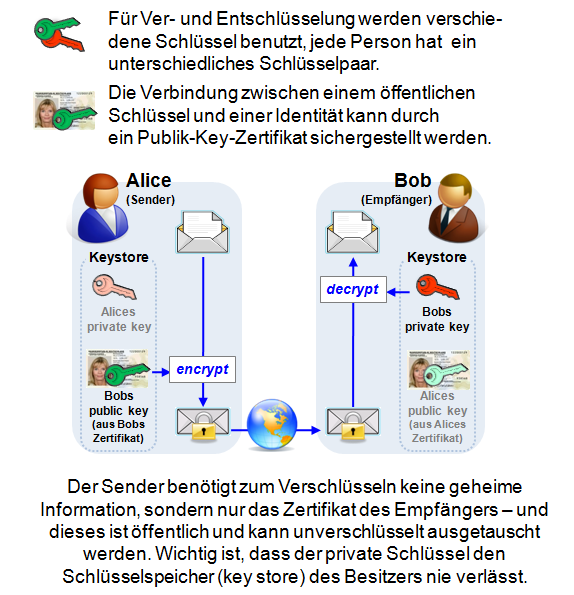
\includegraphics[scale=0.7]{figures/AsymmetricEnc_Figure_Chap1_de.png}
\caption{Asymmetrische oder Public-Key-Verschl�sselung} 
\label{cm_Figure_Asymmetric-Enc_Public-Key-Enc}
\end{center}
\end{figure}

M�chte Alice\index{Alice}%
\footnote{%
  Zur Beschreibung kryptographischer Protokolle werden den Teilnehmern
  oft Namen gegeben (vergleiche \cite[S. 23]{Schneier1996}). 
  Alice und Bob\index{Bob} f�hren alle allgemeinen 2-Personen-Protokolle durch,
  wobei Alice dies initiiert und Bob antwortet.
  Die Angreifer werden als Eve (eavesdropper = passiver Lauscher) und
  Mallory (malicious active attacker = b�swilliger, aktiver Abgreifer)
  bezeichnet.
  }
mit Bob kommunizieren, so sucht sie Bobs �ffentlichen Schl�ssel
und benutzt ihn, um ihre Nachricht an ihn zu
verschl�sseln. Diesen verschl�sselten Text schickt sie dann an Bob,
der mit Hilfe seines geheimen Schl�ssels den Text wieder entschl�s"-seln
kann. Da einzig Bob Kenntnis von seinem geheimen Schl�ssel hat, ist
auch nur er in der Lage, an ihn adressierte Nachrichten zu
entschl�sseln.
Selbst Alice als Absenderin der Nachricht kann aus der von ihr
versandten (verschl�sselten) Nachricht den Klartext nicht wieder
herstellen. Nat�rlich muss sichergestellt sein, dass man aus dem
�ffentlichen Schl�ssel nicht auf den geheimen Schl�ssel schlie�en
kann.\par \vskip + 3pt

% Abbildung evtl. besser hier, wenn Seitenaufteilung ausginge.

Veranschaulichen kann man sich ein solches Verfahren mit einer
Reihe von einbruchssicheren Briefk�sten. Wenn ich eine Nachricht
verfasst habe, so suche ich den Briefkasten\index{Briefkasten} mit dem
Namensschild des Empf�ngers und werfe den Brief dort ein. Danach kann ich die
Nachricht selbst nicht mehr lesen oder ver�ndern, da nur der
legitime Empf�nger im Besitz des Schl�ssels f�r den Briefkasten
ist.\par \vskip + 3pt

Vorteil von asymmetrischen Verfahren ist das einfachere
\index{Schl�sselmanagement} Schl�sselmanagement. Betrachten wir
wieder ein Netz mit $n$ Teilnehmern. Um sicherzustellen, dass
jeder Teilnehmer jederzeit eine verschl�sselte Verbindung zu
jedem anderen Teilnehmer aufbauen kann, muss jeder Teilnehmer ein
Schl�sselpaar besitzen. Man braucht also $2n$ Schl�ssel oder $n$
Schl�sselpaare. Ferner ist im Vorfeld einer �bertragung kein
sicherer Kanal notwendig, da alle Informationen, die zur Aufnahme
einer vertraulichen Kommunikation notwendig sind, offen
�bertragen werden k�nnen. Hier ist lediglich%
\footnote{%
Dass auch dies nicht trivial ist, wird z.B. in Kapitel \ref{nt_Shared-Primes}
erl�utert.
Neben den Anforderungen bei der Schl�sselgenerierung ist zu beachten, dass
inzwischen auch die (Public-Key-)Infrastrukturen selbst Ziel von 
Cyber-Angriffen sind.
}
auf die Unverf�lschtheit (Integrit�t und Authentizit�t)
\index{Authentizit�t} des �ffentlichen Schl�ssels zu achten.
Nachteil: Im Vergleich zu symmetrischen Verfahren sind reine
asymmetrische Verfahren jedoch um ein Vielfaches langsamer.\par \vskip + 3pt

Das bekannteste asymmetrische Verfahren ist der \index{RSA} 
RSA-Algorithmus\index{CrypTool}%
\footnote{%
  RSA wird in diesem Skript ab Kapitel \ref{rsabeweis} ausf�hrlich beschrieben.
  Die aktuellen Forschungsergebnisse im Umfeld von RSA werden in Kapitel
  \ref{SecurityRSA} beschrieben.
}%
, der nach seinen Entwicklern Ronald \index{Rivest, Ronald} Rivest, 
Adi \index{Shamir, Adi} Shamir und Leonard \index{Adleman, Leonard} Adleman
benannt wurde. Der RSA-Algorith"-mus wurde 1978 ver�ffentlicht.\footnote{%
  Hinweise zur Geschichte von RSA und seiner Ver�ffentlichung, die nicht im Sinne
  der NSA war, finden sich in der Artikelserie {\em RSA \& Co. in der Schule:
  Moderne Kryptologie, alte Mathematik, raffinierte Protokolle}.
  Siehe \cite{Witten2006}, S. 55 ff (\glqq Penible L�mmergeier\grqq).
  \index{RSA \& Co. in der Schule}
}
Das Konzept der asymmetrischen Verschl�sselung wurde erstmals
von Whitfield Diffie \index{Diffie, Whitfield}  und 
Martin \index{Hellman, Martin} Hellman in Jahre 1976 vorgestellt. 
Heute spielen auch die Verfahren nach
ElGamal \index{ElGamal, Tahir} eine bedeutende Rolle, vor allem die
\index{Schnorr, Claus-Peter} Schnorr-Varianten im \index{DSA} DSA (Digital
\index{Signatur!digital}\index{DSA-Signatur}\index{Signatur!DSA}
Signature Algorithm).

\noindent Angriffe gegen asymmetrische Verfahren werden behandelt in\\
- Kapitel~ \ref{Chapter_ElementaryNT}: \hyperlink{Chapter_ElementaryNT}{Elementare Zahlentheorie},\\
- Kapitel~ \ref{Chapter_ModernCryptography}:
  \hyperlink{Chapter_ModernCryptography}{Moderne Kryptographie},\\
- Kapitel~ \ref{Chapter_EllipticCurves}:
  \hyperlink{Chapter_EllipticCurves}{Elliptische Kurven} und\\
- Kapitel \ref{Chapter_Dlog-FactoringDead}: \hyperlink{Chapter_Dlog-FactoringDead}
  {Aktuelle Resultate zum L�sen diskreter Logarithmen und zur Faktorisierung}.



% --------------------------------------------------------------------------
\newpage
\section[Hybridverfahren]{Hybridverfahren\footnotemark} 
\footnotetext{%
   In CT1\index{CT1} finden Sie dieses Verfahren �ber das Men�
   {\bf Ver-/Entschl�sseln \textbackslash{} Hybrid}:
   Dabei k�nnen Sie die einzelnen Schritte und ihre Abh�ngigkeiten mit konkreten
   Zahlen nachvollziehen. Die Variante mit RSA als asymmetrischem Verfahren
   ist graphisch visualisiert; die Variante mit ECC nutzt die Standard-Dialoge.
   In beiden F�llen wird AES als symmetrisches Verfahren eingesetzt.\index{AES}\\
   JCT\index{JCT} bietet Hybrid-Verfahren (z.B. ECIES) in der
   Algorithmen-Perspektive an unter {\bf Algorithms \textbackslash{} Hybrid Ciphers}.
}
\label{CM_Hybrid-procedures}
\index{Hybridverfahren}

Um die Vorteile von symmetrischen und asymmetrischen Techniken gemeinsam 
nutzen zu k�nnen, werden (zur Verschl�sselung) in der Praxis meist 
Hybridverfahren \index{Verschl�sselung!hybrid} verwendet.\par \vskip + 3pt

Hier werden die Mengen-Daten mittels symmetrischer Verfahren
verschl�sselt: Der Schl�ssel ist ein vom Absender zuf�llig\footnote{%
   Die Erzeugung zuf�lliger Zahlen\index{Zufall} ist ein wichtiger Bestandteil 
   kryptographisch sicherer Verfahren.\\
   - Mit CT1\index{CT1} k�nnen Sie �ber das Men�
   {\bf Einzelverfahren \textbackslash{} Zufallsdaten erzeugen}
   verschiedene Zufallszahlengeneratoren\index{Zufallsgenerator} (PRNGs) ausprobieren.
   �ber das Men� {\bf Analyse \textbackslash{} Zufallsanalyse} k�nnen Sie
   verschiedene Testverfahren f�r Zufallsdaten auf bin�re Dokumente
   anwenden.\\
   % CT1 konzentriert sich auf kryptographisch starke
   % {\bf Pseudo}zufallszahlengeneratoren. \glqq Echte\grqq~
   % Zufallsquellen werden nur �ber den Aufruf des Secude-Generators einbezogen.\\
   %
   - In CT2\index{CT2} k�nnen Sie im Startcenter
   mit dem Suchstring \glqq Zufall\grqq~Vorlagen (Templates) finden, die
   Zufallsgeneratoren\index{Zufallsgenerator} (PRNGs)
   nutzen. Die PRNGs nutzen intern bspw. Keccak\index{Keccak} oder den
   Linear Congruential Generator (LCG)\index{LCG}. Sie werden dann
   bspw. f�r Schl�sselgenerierung oder Dezimalisierung genutzt.\\
   %
   - JCT\index{JCT} bietet {\bf Pseudo}zufallszahlengeneratoren sowohl
   im Men� {\bf Algorithms \textbackslash{} Random Number Generator} der
   Standard-Perspektive als auch in der Algorithmen-Perspektive an.
}\index{Zufall}
generierter geheimer Sitzungsschl�ssel (session key)\index{Session Key},
der nur f�r diese Nachricht verwendet wird.

Anschlie�end wird dieser Sitzungsschl�ssel mit Hilfe des asymmetrischen
Verfahrens verschl�sselt und zusammen mit der Nachricht an den Empf�nger
�bertragen.

Der Empf�nger kann den Sitzungsschl�ssel mit Hilfe seines geheimen
Schl�ssels bestimmen und mit diesem dann die Nachricht entschl�sseln.

Auf diese Weise profitiert man von dem bequemen Schl�sselmanagement\index{Schl�sselmanagement}
asymmetrischer Verfahren (mit �ffentlichem und privatem Schl�ssel), und
man profitiert von der Schnelligkeit symmetrischer Verfahren, um gro�e
Datenmengen zu verschl�sseln (mit den geheimen Schl�sseln).



% --------------------------------------------------------------------------
\newpage
% \vskip +40 pt

\begin{ctsquote}
    Ein altes Sprichwort, angeblich gepr�gt von der
    US National Security Agency (NSA), sagt:\\
    \glqq Angriffe werden immer besser, niemals schlechter.\grqq\\
    ``Attacks always get better; they never get worse.''
\caption[IETF]{IETF\footnotemark}
\end{ctsquote}
\addtocounter{footnote}{0}\footnotetext{%
  \url{http://tools.ietf.org/html/rfc4270}\index{IETF}\index{NSA}
  }

% --------------------------------------------------------------------------
\section[Kryptoanalyse und symmetrische Chiffren f�r Lehrzwecke]{Kryptoanalyse und symmetrische Chiffren f�r Lehrzwecke\footnotemark} 
\footnotetext{%
  Ein sehr guter Start in die Kryptoanalyse ist das Buch von Mark Stamp \cite{Stamp2007}.
  Ebenfalls gut, aber sehr high-level und nur bezogen auf die Analyse symmetrischer
  Blockchiffren ist der Artikel von Bruce Schneier \cite{Schneier2000}.\\
  Einige der Cipher-Challenges bei \glqq MysteryTwister C3\grqq~
  (\url{http://www.mysterytwisterc3.org}) sind ebenfalls gut f�r Lehrzwecke
  einsetzbar.\index{MTC3}\index{Krypto-Wettbewerb}
}
\label{CM_Analysis-SymCiphers-Educational}
\index{Kryptoanalyse}

Verglichen mit den auf der Zahlentheorie beruhenden Public-Key-Verschl�sselungsverfahren wie RSA, ist die Struktur von AES\index{AES} und den meisten anderen modernen symmetrischen Verschl�sse"-lungsverfahren (wie DES, IDEA oder Present) sehr komplex und kann nicht so einfach wie RSA\index{RSA} erkl�rt werden.

Deshalb wurden zu Lehrzwecken vereinfachte Varianten moderner
symmetrischer Verfahren entwickelt, um Einsteigern die M�glichkeit zu geben,
Ver- und Entschl�sselung von Hand zu lernen und ein besseres Verst�ndnis zu
gewinnen, wie die Algorithmen im Detail funktionieren.
Diese vereinfachten Varianten helfen auch, die entsprechenden
Kryptoanalyse-Methoden zu verstehen und anzuwenden.

Die bekanntesten Varianten sind SDES (Simplified DES)%
\footnote{
  Visualisierung: Macht man in CT2\index{CT2} einen Doppelklick auf den Titel der
  SDES-Komponente, ist in der Fullscreen-Ansicht
  % fullscreen
  % in der Fullscreen-Ansicht  %% das gab eine Zeile zuviel und r�ckte 1.7. weiter.
  zu sehen, wie die Bits der eingegebenen Daten durch den Algorithmus flie�en.
  Ein Screen\-shot dazu:
  \url{https://www.facebook.com/CrypTool2/photos/a.505204806238612.1073741827.243959195696509/597354423690316}
}
und S-AES (Simplified-AES) von Prof. Ed Schaefer und seinen Studenten%
\footnote{
    Siehe auch den Artikel \glqq Devising a Better Way to Teach and Learn
    the Advanced Encryption Standard\grqq~unter
    \url{http://math.scu.edu/~eschaefe/getfile.pdf}
    % be_2016-07-17: dead link /toter Link: http://www.scu.edu/cas/research/cryptography.cfm
},
und Mini-AES (siehe das Kapitel~\ref{CM_Sage_Mini-AES} \glqq \nameref{CM_Sage_Mini-AES}\grqq):

\index{DES}\index{DES!SDES}\index{IDEA}\index{AES!Mini-AES}\index{AES!S-AES}
\begin{itemize}

\item Edward F. Schaefer: {\em A Simplified Data Encryption Standard Algorithm} 
      \cite{Schaefer1996}.

\item Raphael Chung-Wei Phan: {\em Mini Advanced Encryption Standard (Mini-AES):
                                   A Testbed for Cryptanalysis Students} 
      \cite{Phan2002}.

\item Raphael Chung-Wei Phan: {\em Impossible differential cryptanalysis of Mini-AES} 
      \cite{Phan2003}.

\item Mohammad A. Musa, Edward F. Schaefer, Stephen Wedig:
      {\em A simplified AES algorithm and its linear and differential cryptanalyses} 
      \cite{Musa2003}.

\item Nick Hoffman: {\em A SIMPLIFIED IDEA ALGORITHM} 
      \cite{Hoffman2006}.

\item S. Davod. Mansoori, H. Khaleghei Bizaki: 
      {\em On the vulnerability of Simplified AES Algorithm Against Linear Cryptanalysis} 
      \cite{Mansoori2007}.

\end{itemize}



% --------------------------------------------------------------------------
\section{Weitere Informationsquellen}

Neben den anderen Kapiteln in diesem Skript, der umfangreichen Fachliteratur
und vielen Stellen im Internet enth�lt auch die Online-Hilfe aller 
CrypTool-Varianten\index{CrypTool} sehr viele weitere Informationen zu den 
einzelnen symmetrischen und asymmetrischen Verschl�sselungsverfahren.




% ---------------------------------------------------------------------------
% ---------------------------------------------------------------------------
\newpage
\hypertarget{CM_Appendix_SageCode}{}
\section{Anhang: Beispiele mit SageMath}
\label{CM_Sage_samples}
\index{SageMath!Programmbeispiele}

\noindent Der folgende Abschnitt enth�lt SageMath Source-Code, der sich auf den
Inhalt des Kapitels~\ref{CM_Analysis-SymCiphers-Educational}
(\glqq \nameref{CM_Analysis-SymCiphers-Educational}\grqq) bezieht.

Weitere Details zu in SageMath enthaltenen Kryptoverfahren (z.B. zum Simplified
Data Encryption Standard SDES) finden sich z.B. in der Diplomarbeit von Minh Van
Nguyen \cite{Nguyen2009b}.

% ---------------------------------------------------------------------------
\subsection{Mini-AES}
\label{CM_Sage_Mini-AES}
\index{AES!Mini-AES}

Das SageMath-Modul \texttt{crypto/block\_cipher/miniaes.py} enth�lt den Mini-AES, mit
dem Studenten die Funktionsweise moderner Blockchiffren untersuchen k�nnen.

Mini-AES, urspr�nglich vorgestellt von \cite{Phan2002}, ist eine vereinfachte
Variante des Advanced Encryption Standard (AES) f�r Ausbildungszwecke.

Wie man Mini-AES benutzt, ist ausf�hrlich in der SageMath Reference-Page beschrieben:
\begin{sloppypar} % N�tig, da sonst ein schwarzer Punkt
  \url{http://doc.sagemath.org/html/en/reference/cryptography/sage/crypto/block_cipher/miniaes.html}.
\end{sloppypar}

Das folgende SageMath-Code-Beispiel~\ref{cm_Mini-AES:Sage_example}
ist aus den Release-Notes von SageMath 4.1%
\footnote{
  Siehe \url{http://mvngu.wordpress.com/2009/07/12/sage-4-1-released/}.\\
  Weiterer Beispiel-Code zum Mini-AES findet sich in
  \cite[Kap. 6.5 und Anhang D]{Nguyen2009a}.
}
und ruft diese Implementierung des Mini-AES auf.


% Using [fontsize=\footnotesize,fontshape=tt] caused:
%   LaTeX Font Warning: Font shape `T1/cmtt/m/tt' undefined
%   (Font)              using `T1/cmtt/m/n' instead on input line 730.
% so deleted the fontshape parameter.
\begin{sagecode}
\begin{Verbatim}%
[fontsize=\footnotesize]
# We can encrypt a plaintext using Mini-AES as follows:
sage: from sage.crypto.block_cipher.miniaes import MiniAES
sage: maes = MiniAES()
sage: K = FiniteField(16, "x")
sage: MS = MatrixSpace(K, 2, 2)
sage: P = MS([K("x^3 + x"), K("x^2 + 1"), K("x^2 + x"), K("x^3 + x^2")]); P

[  x^3 + x   x^2 + 1]
[  x^2 + x x^3 + x^2]
sage: key = MS([K("x^3 + x^2"), K("x^3 + x"), K("x^3 + x^2 + x"), K("x^2 + x + 1")]); key

[    x^3 + x^2       x^3 + x]
[x^3 + x^2 + x   x^2 + x + 1]
sage: C = maes.encrypt(P, key); C

[            x       x^2 + x]
[x^3 + x^2 + x       x^3 + x]

# Here is the decryption process:
sage: plaintxt = maes.decrypt(C, key)
sage: plaintxt == P
True

# We can also work directly with binary strings:
sage: from sage.crypto.block_cipher.miniaes import MiniAES
sage: maes = MiniAES()
sage: bin = BinaryStrings()
sage: key = bin.encoding("KE"); key
0100101101000101
sage: P = bin.encoding("Encrypt this secret message!")
sage: C = maes(P, key, algorithm="encrypt")
sage: plaintxt = maes(C, key, algorithm="decrypt")
sage: plaintxt == P
True

# Or work with integers n such that 0 <= n <= 15:
sage: from sage.crypto.block_cipher.miniaes import MiniAES
sage: maes = MiniAES()
sage: P = [n for n in xrange(16)]; P
[0, 1, 2, 3, 4, 5, 6, 7, 8, 9, 10, 11, 12, 13, 14, 15]
sage: key = [2, 3, 11, 0]; key
[2, 3, 11, 0]
sage: P = maes.integer_to_binary(P)
sage: key = maes.integer_to_binary(key)
sage: C = maes(P, key, algorithm="encrypt")
sage: plaintxt = maes(C, key, algorithm="decrypt")
sage: plaintxt == P
True
\end{Verbatim}
\caption{Ver- und Entschl�sselung mit dem Mini-AES}
\label{cm_Mini-AES:Sage_example}
\end{sagecode}
\clearpage%% Um das Codebeispiel vor das ff. Kap. 1.8.2 zu bekommen.


% ---------------------------------------------------------------------------
\subsection{Weitere symmetrische Krypto-Algorithmen in SageMath}
\label{CM_Sage_SymCryptoAlg}

Die Referenz zu SageMath v7.2 f�hrt als kryptographische Funktionen u.a. auf:%
\footnote{
  Siehe 
  \url{http://doc.sagemath.org/html/en/reference/sage/crypto/index.html},\\
  \url{http://doc.sagemath.org/html/en/reference/cryptography/index.html} und\\
  \url{http://combinat.sagemath.org/doc/reference/cryptography/sage/crypto/stream.html}
}
\begin{itemize}
   \item Linear feedback shift register (LFSR),
   \item Blum-Blum-Shub (BBS): Pseudo-Zufallsbit-Generator (zu finden bei Streams),
   \item Gitter-basierte Funktionen.
% be_2016-07-17: Nicht mehr gefunden in Refrence 7.2:
% - ShrinkingGeneratorCryptosystem,
\end{itemize}



%------------------------------------------------------------------------------
\putbib[../de/references]
\addcontentsline{toc}{section}{Literaturverzeichnis}
\end{bibunit}

\noindent Alle Links wurden am 10.07.2016 �berpr�ft.



% --------------------------------------------------------------------------
\newpage
\chapter*{Web-Links}\addcontentsline{toc}{section}{Web-Links}

\begin{enumerate}

  \hypertarget{CM_HT_Weblink_Rijndael-Cryptosystem}{}
  \item \glqq AES Discussion Groups\grqq~beim NIST (archive page provided for historical purposes, last update on Feb 28th, 2001)\\
	% \grqq nach \item braucht die Tilde, aber kein weiteres Blank.
	%  Sonst reicht ein Blank, wenn ein weiteres Wort danach folgt
	%  (es reicht auch nicht, wenn danach ein Zeilenumbruch).
	\url{http://csrc.nist.gov/archive/aes/}

  \item Das AES-/Rijndael-Kryptosystem (page maintained by Nicolas T. Courtois, last update on Aug 24th, 2007)\\
        \url{http://www.cryptosystem.net/aes}

  \item distributed.net:~\glqq RC5-64 has been solved\grqq\\
        \url{http://www.distributed.net/Pressroom_press-rc5-64}

	% \begin{sloppypar}  ... \end{sloppypar} worked. Get rid of \\ before to avoid extra newline.
\item RSA Labs (ehemals RSA Security): ~\glqq The RSA Secret Key Challenge\grqq
        \begin{sloppypar}
	\url{https://www.emc.com/emc-plus/rsa-labs/historical/the-rsa-laboratories-secret-key-challenge.htm}
	\end{sloppypar}

  \item RSA Labs (ehemals RSA Security): ~\glqq DES Challenge\grqq\\
        \url{https://www.emc.com/emc-plus/rsa-labs/historical/des-challenge-iii.htm}

  \item Weiterf�hrende Links auf der CrypTool-Homepage\\
        \url{http://www.cryptool.org}
	       
\end{enumerate}

Alle Links wurden am 10.07.2016 �berpr�ft.



% Local Variables:
% TeX-master: "../script-de.tex"
% End:

% $Id$
%%%%%%%%%%%%%%%%%%%%%%%%%%%%%%%%%%%%%%%%%%%%%%%%%%%%%%%%%%%%%%%%%%%%%%%%%%
%
% C H A P T E R   T H R E E :  P R I M E S
%
%%%%%%%%%%%%%%%%%%%%%%%%%%%%%%%%%%%%%%%%%%%%%%%%%%%%%%%%%%%%%%%%%%%%%%%%%%

\newpage
% \hypertarget{Kapitel_2}{}
\chapter{Prime Numbers}
\label{Label_Kapitel_Primes}
(Bernhard Esslinger, May 1999; Updates Nov. 2000, Dec. 2001, June 2003, May 2005, March 2006, June 2007, Jan. 2010, Dec. 2012)

\begin{ctsquote}
    Progress requires exchange of knowledge.
\caption[Albert Einstein]{Albert Einstein\footnotemark}
\end{ctsquote}
\addtocounter{footnote}{0}\footnotetext{%
  Albert Einstein, German physicist and Nobel Prize winner, 
  Mar 14, 1879 $-$ Apr 14, 1955.
}

% --------------------------------------------------------------------------
\section{What are prime numbers?}
\index{Prime number} \index{Number!prime}
Prime numbers are whole, positive numbers greater than or equal to $2$ that can
only be divided by 1 and themselves. All other natural numbers (composite
numbers) can be formed by multiplying prime numbers.

\noindent The {\em natural} \index{Number!natural} numbers
$\mathbb{N}=\{1, 2, 3, 4,\cdots \}$ thus comprise 
\begin{itemize}
   \item the number $1$ (the unit value)
   \item the primes and
   \item the composite numbers.
\end{itemize}

\noindent Prime numbers are particularly important for three reasons:
\begin{itemize}
  \item In number theory, they are considered to be the basic components of
natural numbers, upon which numerous brilliant mathematical ideas are based.
  \item They are of extreme practical importance in modern
\index{Cryptography!modern} cryptography (public key \index{Cryptography!public key} cryptography). The most common public key procedure, invented at the end of
the 1970's, is \index{RSA} RSA encryption. Only using (large) prime numbers for
particular parameters can you guarantee that an algorithm is secure, both for
the RSA procedure and for even more modern procedures (e.g. elliptic curves).
  \item The search for the largest known prime numbers does not have any
practical usage known to date, but requires the best computers, is an excellent
benchmark (possibility for determining the performance\index{Performance} of computers) and leads
to new calculation methods on many computers \\
(see also: \url{http://www.mersenne.org/prime.htm}).
\end{itemize}
Many people have been fascinated by prime numbers over the past two millennia.
Ambition to make new discoveries about prime numbers has often resulted in
brilliant ideas and conclusions. The following section provides an easily
comprehensible introduction to the basics of prime numbers. We will also
explain what is known about the distribution (density, number of prime numbers
in particular intervals) of prime numbers and how prime number tests work.


% --------------------------------------------------------------------------
\section{Prime numbers in mathematics}\label{primesinmath}

Every whole number has a factor. The number 1 only has one factor,
itself, whereas the number $12$ has the six factors $1, 2, 3, 4,
6, 12$. Many numbers can only be divided by themselves and by $1$.
With respect to multiplication, these are the ``atoms'' in the
area of numbers. Such numbers are called prime numbers.

In mathematics, a slightly different (but equivalent) definition is used.

\begin{definition}\label{def-pz-prime}
A whole number $p \in {\bf N}$ is called prime \index{Number!prime} if
$p > 1$ and $p$ only possesses the trivial factors $\pm 1$ and $\pm p$.
\end{definition}


By definition, the number $1$ is not a prime number. In the following sections,
$p$ will always denote a prime number.

The sequence of prime numbers starts with $$ 2,~ 3,~ 5,~ 7, ~ 11, ~ 13, ~
17, ~ 19, ~ 23, ~ 29, ~ 31, ~ 37, ~ 41, ~ 43, ~ 47, ~ 53, ~ 59, ~ 61,
~ 67, ~ 71, ~ 73, ~ 79, ~ 83, ~ 89, ~ 97, \cdots . $$
The first 100 numbers include precisely 25 prime numbers. After this,
the percentage of primes constantly decreases. Prime numbers can be
factorized in a uniquely {\em trivial} way: 
$$5 = 1 \cdot 5,\quad  17 = 1 \cdot 17, \quad 1013 = 1 \cdot 1013,  \quad
1,296,409 = 1 \cdot 1,296,409.$$
All numbers that have $2$ or more factors not equal 1 are called 
\index{Number!composite} {\em composite} numbers. 
These include $$ 4 = 2 \cdot 2, \quad 6 = 2\cdot 3 $$ as well
as numbers that {\em look like primes}, but are in fact composite:
$$ 91 = 7 \cdot 13, \quad 161=7 \cdot 23, \quad 767 =13 \cdot 59. $$

\begin{theorem}\label{thm-pz-sqr}
Each whole number $m$ greater than $1$ possesses a lowest factor greater than
$1$. This is a prime number $p$. Unless $m$ is a prime number itself, then: $p$
is less than or equal to the square root of $m$.
\end{theorem}

All whole numbers greater than $1$ can be expressed as a product of prime
numbers --- in a unique way. This is the claim of the \textbf{1st fundamental theorem of
number theory} (= fundamental theorem of arithmetic = fundamental building block
of all positive integers).\index{Number theory!fundamental theorem}

\begin{theorem}\label{thm-pz-prod}
Each element $n$ of the natural numbers greater than $1$ can be written as the
product $n = p_1 \cdot p_2 \dots p_m$ of prime numbers. If two such
factorizations $$n =  p_1 \cdot p_2 \cdot \cdots \cdot p_m = p'_1 \cdot p'_2 \cdots
p'_{m'}$$ are given, then they can be reordered such that $\;m = m'\;$ and for
all $i$:  $\;p_i = p'_i$. \\
($p_1, p_2, \dots, p_m$ are called the prime factors of n).
\end{theorem}

In other words: each natural number other than $1$ can be written as a product
of prime numbers in precisely one way, if we ignore the order of the factors.
The factors are therefore unique (the {\em expression as a product of factors}
is unique)! For example, $$ 60 = 2 \cdot 2 \cdot 3 \cdot 5 = 2^2\cdot 3^1 \cdot
5^1. $$
And this --- other than changing the order of the factors --- is the only way in
which the number $60$ can be factorized. If you allow numbers other than primes
as factors, there are several ways of factorizing integers and the \textbf{uniqueness} \hypertarget{uniqueness}{} is
lost: $$ 60 = 1 \cdot 60 = 2 \cdot 30 = 4 \cdot 15 = 5 \cdot 12 =6 \cdot 10 = 2
\cdot 3 \cdot 10 = 2 \cdot 5 \cdot 6 = 3 \cdot 4 \cdot 5 = \cdots . $$

The following section is aimed more at those familiar with mathematical logic:
The 1st fundamental theorem only appears to be obvious \label{remFundTheoOfArithm}. We can construct
numerous other sets of numbers (i.e. other than positive whole numbers greater
than 1), for which numbers in the set cannot be expressed uniquely as a product
of the prime numbers of the set: In the set $M = \{1, 5, 10, 15, 20, \cdots\}$
there is no equivalent to the fundamental theorem under multiplication. The
first five prime numbers of this sequence are $5, 10, 15, 20, 30$ (note: $10$ is
prime, because $5$ is not a factor of $10$ in this set --- the result is not an
element of the given basic set $M$). Because the following applies in $M$: $$
100 = 5 \cdot 20 = 10 \cdot 10 $$ and $5, 10, 20$ are all prime numbers in this
set, the expression as a product of prime factors is not unique here.

% --------------------------------------------------------------------------
\section{How many prime numbers are there?}

For the natural numbers, the primes can be compared to elements in chemistry or
the elementary particles in physics (see \cite[p. 22]{pr:Blum1999}).

Although there are only $92$ natural chemical elements, the number of prime
numbers is unlimited. Even the Greek, \index{Euclid} Euclid%
\footnote{Euclid,
a Greek mathematician of 4th and 3rd century B.C. He worked at the
Egyptian academy of Alexandria and wrote ``The Elements'', the most well 
known systematically textbook of the Greek mathematics.} 
knew this in the third century B.C.
\begin{theorem}[Euclid\footnote{The common usage of the term does not denote Euclid as the inventor of the theorem rather;
the true inventor is merely not as prominent. The theorem has already been distinguished
and proven in Euclid's Elements (Book IX, theorem 20). The phraseology is remarkable due to 
the fact that the word infinite is not used. The text reads as followed
$$
O\acute{\iota}~\pi\varrho\tilde{\omega}\tau o \iota~\grave{\alpha}\varrho\iota\vartheta\mu o\grave{\iota}~
\pi\lambda\varepsilon\acute{\iota}o \upsilon\varsigma~\varepsilon\grave{\iota}\sigma\grave{\iota}~
\pi\alpha\nu\tau\grave{o}\varsigma~\tau o \tilde{\upsilon}~
\pi\varrho o \tau\varepsilon\vartheta\acute{\varepsilon}\nu\tau o \varsigma~
\pi\lambda\acute{\eta}\vartheta\ o \upsilon\varsigma~
\pi\varrho\acute{\omega}\tau\omega\nu~
\grave{\alpha}\varrho\iota\vartheta\mu\tilde{\omega}\nu,
$$
the English translation of which is: the prime numbers are more than 
any previously existing amount of prime numbers.
}]\label{thm-pz-euklid} % Ende der Fu�note
% Fussnote VOR "]" in [Euclid], damit kein Leerraum vor der Fussnotennummer.
% Vorher stand da: ...(Euclid). BLANK Fussnote und das Blank stoerte.
% Nun steht die Fussnote direkt hinter "Euclid" und vor der ")".
% Eigentlich h�tte ich sie gerne direkt hinter "(Euclid)", noch vor dem 
% automatisch gesetzten Punkt. 
The sequence of prime numbers does not discontinue.
Therefore, the quantity of prime numbers is infinite.
\end{theorem}
His proof that there is an infinite number of
primes is still considered to be a brilliant mathematical consideration and
conclusion today (\textbf{proof by contradiction} \index{Proof by contradiction}). 
He assumed that there is only a finite number of primes and therefore a 
largest prime number. Based on this assumption, he drew logical conclusions
until he obtained an obvious contradiction. This meant that something must
be wrong. As there were no mistakes in the chain of conclusions, it could
only be the assumption that was wrong. Therefore, there must be an infinite
number of primes!\\

\hypertarget{euclid}{}
\index{Euclid's proof by contradiction}\index{Proof by contradiction}
% \paragraph*{Euclid's proof by contradiction}
% goes as follows:
\begin{Proof}{according to Euclid (proof by contradiction)\\}
{\bf Assumption:} \quad There is a {\em finite} number of primes. \\*[4pt] {\bf
Conclusion:} \quad Then these can be listed $p_1 < p_2 < p_3 < \dots < p_n$,
where $n$ is the (finite) number of prime numbers. $p_n$ is therefore the
largest prime. Euclid now looks at the number $a = p_1 \cdot p_2 \cdots p_n +1$.
This number cannot be a prime number because it is not included in our list of
primes. It must therefore be divisible by a prime, i.e. there is a natural
number $i$ between $1$ and $n$, such that $p_i$ divides the number $a$. Of
course, $p_i$ also divides the product $a-1 = p_1 \cdot p_2 \cdots p_n$, because
$p_i$ is a factor of $a-1$. Since $ p_i $ divides the numbers $ a $ and $ a-1 $,
it also divides the difference of these numbers. Thus: $p_i$ divides  $a - (a-1)
= 1$. $p_i$ must therefore divide $1$, which is impossible. \\*[4pt] {\bf
Contradiction:} \quad Our assumption was false.

Thus there is an {\em infinite} number of primes
(Cross-reference: \hyperlink{primhfk}{overview} under \ref{s:primhfk} of 
the number of prime numbers in various intervals).
\end{Proof} 

\par \vskip + 10pt

Here we should perhaps mention yet another fact which is initially somewhat surprising. 
Namely, in the prime numbers sequence $p_1, p_2, \cdots,$ gaps between prime numbers can have
an individually determined length $n$. It is undeniable that under the $n$
succession of natural numbers
$$(n+1)!+2,\cdots, (n+1)!+(n+1),
$$
none of them is a prime number since in order, the numbers $2,3,\cdots,(n+1)$  
are comprised respectively as real divisors. 
($n!$ means the product of the first $n$ natural numbers therefore 
$ n!= n*(n-1)*\cdots *2*1$).


% --------------------------------------------------------------------------
% --------------------------------------------------------------------------
\vskip + 20pt
\section{The search for extremely large primes}
\label{search_for_very_big_primes}   % chap. 3.4

The largest prime numbers known today have several millions digits, 
which is too big for us to imagine. The number of elementary particles in
the universe is estimated to be ``only'' a $80$-digit number 
\hyperlink{grosord}{(See: overview under \ref{s:grosord}
of various orders of magnitude / dimensions)}.


% --------------------------------------------------------------------------
\hypertarget{RecordPrimes}{}
\subsection{The 20+ largest known primes (as of July 2012)}  % Eyecatcher_neue-Mersenne
\label{RecordPrimes}
\index{Prime number!records}

The following table contains the biggest, currently known primes and
a description of its particular number type\footnote{%
An up-to-date version can be found in the internet at
     \url{http://primes.utm.edu/largest.html}
and at
     \url{http://primes.utm.edu/mersenne/index.html}.
}:

\index{Mersenne!number!generalized}
\index{Fermat!number!generalized} 

\begin{table} % don't use [h] (error if table has >24 lines)
\begin{center}
\begin{tabular}{|c|cccc|}
\hline    % Eyecatcher_neue-Mersenne
	& {\bf Definition} & {\bf Decimal Digits} & {\bf When} & {\bf Description} \\
\hline
	1  & $2^{43,112,609}-1$ & 12,978,189 & 2008 & Mersenne, 47th known \\
	2  & $2^{42,643,801}-1$ & 12,837,064 & 2009 & Mersenne, 46th known \\
	3  & $2^{37,156,667}-1$ & 11,185,272 & 2008 & Mersenne, 45th known \\

	4  & $2^{32,582,657}-1$ &  9,808,358 & 2006 & Mersenne, 44th known \\
	5  & $2^{30,402,457}-1$ &  9,152,052 & 2005 & Mersenne, 43rd known \\
	6  & $2^{25,964,951}-1$ &  7,816,230 & 2005 & Mersenne, 42nd known \\
	7  & $2^{24,036,583}-1$ &  7,235,733 & 2004 & Mersenne, M-41 \\
	8  & $2^{20,996,011}-1$ &  6,320,430 & 2003 & Mersenne, M-40 \\
	9  & $2^{13,466,917}-1$ &  4,053,946 & 2001 & Mersenne, M-39 \\
	10 & $19,249 \cdot 2^{13,018,586}+1$ & 3,918,990 & 2007 & Generalized Mersenne\footnotemark \\
	11 & $27,653 \cdot 2^{9,167,433}+1$ & 2,759,677 & 2005 & Generalized Mersenne \\



	12 & $28,433 \cdot 2^{7,830,457}+1$ & 2,357,207 & 2004 & Generalized Mersenne \\

	13  & $2^{ 6,972,593}-1$ & 2,098,960 & 1999 & Mersenne, M-38 \\
	14  & $5,359 \cdot 2^{5,054,502}+1$ & 1,521,561 & 2003 & Generalized Mersenne \\

	15  & $4,847 \cdot 2^{3,321,063}+1$ & 999,744 & 2005 & Generalized Mersenne \\
	16  & $3 \cdot 2^{3,136,255}-1$ & 944,108 & 2007 & Generalized Mersenne \\

	17  & $2^{ 3,021,377}-1$ &   909,526 & 1998 & Mersenne, M-37 \\
	18  & $2^{ 2,976,221}-1$ &   895,932 & 1997 & Mersenne, M-36 \\

	19  & $222,361 \cdot 2^{2,854,840}+1$ & 859,398 & 2006 & Generalized Mersenne \\

	20 & $1,372,930^{131,072}+1$ &   804,474 & 2003 & Generalized Fermat\footnotemark \\

	21  & $1,361,244^{131,072}+1$ &   803,988 & 2004 & Generalized Fermat \\
	22  & $1,176,694^{131,072}+1$ &   795,695 & 2003 & Generalized Fermat \\

	23  & $342,673 \cdot 2^{2,639,439}-1$ & 794,556 & 2007 & Generalized Mersenne \\

\hline
\end{tabular}
\caption{The 20+ largest known primes and its particular number types
         (as of July 2012)}    % Eyecatcher_neue-Mersenne
\label{L_n_Largest_Known-Primes}
\end{center}
\end{table} 
\addtocounter{footnote}{-1}
\footnotetext{\index{Number!Sierpinski}\index{Seventeen or Bust SoB}%
This number was found within the distributed computing project
``Seventeen or Bust'' (SoB) (\url{http://www.seventeenorbust.com})
% {\href{http://www.mersenne.org} {\tt http://www.mersenne.org}}
at March 26, 2007. While the well known \hyperlink{GIMPS-project}{GIMPS project} (chapter~\ref{zahlentyp_mersenne}) searches for bigger and bigger of the infinitely many primes, there is a chance, that the SoB project could have been completed its task sometime.

The SoB project tries to prove computationally, that the number $k = 78,557$ is
the smallest Sierpinski number (John Selfridge proved in 1962, that $78,557$ is a Sierpinski number).

The famous Polish mathematician Waclaw Sierpinski (1882 to 1969) proved in
1960, that there exist infinitely many odd integers k, which fulfill the
following property: For all Sierpinski numbers k it is true: All numbers $N = k \cdot 2^{n}+1$ are composite for all integers $n>=1$ (Sierpinski's Composite Number Theorem, \url{http://mathworld.wolfram.com/SierpinskisCompositeNumberTheorem.html}).

When the project started in 2002 there have been 17 possible candidates $< 78557$ (this is the reason for the project's name ``Seventeen or Bust''). It is sufficient to find one single counter-example, to exclude a candidate k, which means to find a single $n>=1$, where $N = k \cdot 2^{n}+1$ is prime. So it is only a byproduct of this task that this also generates new monster primes.
} 
\addtocounter{footnote}{1}
\footnotetext{%
Generalized Fermat number: $ 1,372,930^{131,072} + 1 = 1,372,930^{(2^{17})}+1 $
\index{Fermat!number!generalized}  } 
%be_2005: Erzwingen, dass die Abb. noch in diesem Kapitel !

The largest known prime is a Mersenne prime, found by the
\hyperlink{GIMPS-project}{GIMPS project}(chapter~\ref{zahlentyp_mersenne}).

Within the largest known primes there are also numbers of the type
\hyperlink{generalizedMersennenumbers}{generalized Mersenne number}
(chapter~\ref{generalized-mersenne-no1})
and 
\hyperlink{generalizedFermatprimes}{generalized Fermat numbers}
(chapter~\ref{generalized-fermat}).


% --------------------------------------------------------------------------
\hypertarget{MersenneNumbers01}{}
\subsection{Special number types -- Mersenne numbers and Mersenne primes} 
\label{zahlentyp_mersenne}
\index{Mersenne!number}

Almost all known huge prime numbers are special candidates, called
\index{Mersenne, Marin} {\em Mersenne numbers}\footnote{%
Marin Mersenne, French priest and mathematician, Sep 08, 1588 $-$ Sep 01, 1648.
\index{Mersenne, Marin}
}
of the form $2^p -1,$ where $p$ is
a prime. Not all Mersenne numbers are prime:

$$
\begin{array}{cl}
2^2 - 1 = 3 & \Rightarrow {\rm prime} \\
2^3 - 1 = 7 & \Rightarrow {\rm prime} \\
2^5 - 1 = 31    & \Rightarrow {\rm prime} \\
2^7 - 1 = 127    & \Rightarrow {\rm prime} \\
2^{11} - 1 = 2,047 = 23 \cdot 89    & \Rightarrow  {\rm NOT~prime} !
\end{array}
$$

\index{Number!Mersenne}\index{Mersenne!number}
\index{Mersenne!theorem} 

Even Mersenne knew that not all Mersenne numbers
are prime (see exponent $p = 11$). 
A prime Mersenne number \index{Mersenne!prime number} is called
Mersenne prime number.  \\
However, he is to be thanked for the interesting conclusion that a number 
of the form $2^n-1$ cannot be a prime number if $n$ is a composite number:

\begin{theorem}[Mersenne]\label{thm-pz-mersenne} 
  If $2^n - 1$ is a prime number, then $n$ is also a prime number.
\end{theorem}

\begin{Proof}{}
The theorem of Mersenne can be proved by contradiction%
\index{Proof by contradiction}.  We therefore assume that
there exists a composite natural number $ n $ (with real factorization)  
$ n=n_1 \cdot n_2 $
, with the property that $ 2^n -1 $ is a prime number.

From \begin{eqnarray*} (x^r-1)((x^r)^{s-1} + (x^r)^{s-2} + \cdots + x^r +1) & =
&  ((x^r)^s + (x^r)^{s-1} + (x^r)^{s-2} + \cdots + x^r) \\ &  & -((x^r)^{s-1} +
(x^r)^{s-2} + \cdots + x^r +1)  \\ & = & (x^r)^s -1 = x^{rs } -1,
\end{eqnarray*} we conclude \[ 2^{n_1 n_2} - 1 = (2^{n_1} -1)((2^{n_1})^{n_2 -1}
+ (2^{n_1})^{n_2 -2} + \cdots + 2^{n_1} + 1). \]
Because $ 2^n - 1 $ is a prime number, one of the above two factors on the
right-hand side must be equal to 1. This is the case if and only if $ n_1 =1 $
or $ n_2 =1$. But this contradicts our assumption. Therefore the assumption is
false. This means that there exists no composite number $ n, $ such that $ 2^n -
1 $ is a prime.
\end{Proof} 

\vskip + 5pt
\hypertarget{Mer-nums-not-always-prim}{}
Unfortunately this theorem only applies in one direction (the inverse 
statement does not apply, no equivalence): that means that there exist 
prime exponent for which the Mersenne number is {\bf not} prime (see the 
above example $2^{11}-1, $ where $11$ is prime, but $2^{11}-1$ not).

Mersenne claimed that $2^{67}-1$ is a prime number. There is also a mathematical
history behind this claim: it first took over 200 years before 
\index{Lucas, Edouard} Edouard Lucas (1842-1891) proved that this number 
is composite.
However, he argued indirectly and did not name any of the factors. In 1903,
Cole\index{Cole, Frank Nelson}\footnote{%
Frank Nelson Cole, American mathematician, Sep. 20, 1861 $-$ May 26, 1926.}
showed which factors make up this composite number: 
$$ 2^{67} -1
=147, 573, 952, 589, 676, 412, 927 = 193, 707, 721 \cdot 761, 838, 257, 287. $$
He admitted to having worked 20 years on the factorization 
\index{Factorization} (expression as a product of prime factors)\footnote{%
  Using CT1\index{CrypTool 1} you can factorize numbers in the 
  following way: menu {\bf Indiv. Procedures \textbackslash{} RSA Cryptosystem 
  \textbackslash{} Factorization of a Number}. \\
  CT1 can factorize with the quadratic sieve (QS) on a single PC in a reasonable
  time numbers no longer than 250 bit.
  Numbers bigger than 1024 bits are currently not accepted by CT1. \\
  With CT2 you can use both the QS and the GNFS (general number field sieve),
  and CT2 can distribute the calculations on several computers.\\
  The current factorization records are listed in chapter \ref{nt:NoteFactorization}.
  \index{Factorization!factoring records}
}
of this 21-digit decimal number!

Due to the fact that the exponents of the Mersenne numbers
\index{Mersenne!number} do not use all
natural numbers, but only the primes, the {\em experimental space} is limited
considerably. The currently known Mersenne prime numbers 
\index{Mersenne!prime number} have the exponents\footnote{%
Landon Curt Noll\index{Noll, Landon Curt} lists all known Mersenne primes
including its date of discovery and its value as number and as word:
      \url{http://www.isthe.com/chongo/tech/math/prime/mersenne.html} \\
Also see:
      \url{http://www.utm.edu/}.
                             } 
$$
\begin{array}{c}
2; ~ 3; ~ 5; ~ 7; ~ 13; ~ 17; ~ 19; ~ 31; ~ 61; ~ 89; ~ 107; ~ 127;
~ 521; ~ 607; ~ 1,279; ~ 2,203; ~ 2,281; ~ 3,217;\\
4,253; ~ 4,423; ~ 9,689; ~ 9,941, ~ 11,213; ~ 19,937; ~ 21,701; ~ 23,207; ~ 44,497; ~
86,243; ~ 110,503; \\
132,049; ~ 216,091; ~ 756,839; ~ 859,433; ~ 1,257,787; ~ 1,398,269; ~ 2,976,221; ~ 3,021,377;\\
6,972,593; ~ 13,466,917; ~ 20,996,011; ~ 24,036,583; ~ 25,964,951; ~ 30,402,457;\\
32,582,657; ~ 37,156,667; ~ 42,643,801, ~ 43,112,609.
% be_2005_UPDATEN_if-new-mersenne-prime-appears          ~ xxx,xxx,xxx.
\end{array}
$$
Thus    % Eyecatcher_neue-Mersenne
$47$            % be_2005_UPDATEN_if-new-mersenne-prime-appears
Mersenne prime numbers are currently known%
\index{Prime number!Mersenne}\index{Mersenne!prime number}. 

The $19$th number with the exponent $4,253$ was the first with at least $1,000$ digits in  decimal system
(the mathematician Samual \index{Yates, Samual} Yates coined the expression {\em
titanic} \index{Prime number!titanic} prime for this; it was discovered by
Hurwitz in 1961); the $27$th number with the exponent $44,497$ was the first
with at least $10,000$ digits in the decimal system (Yates coined the expression
\index{Prime number!gigantic}  {\em gigantic} prime for this. These names are
now long outdated).


\vskip +10 pt
For the first 41            % be_2005_UPDATEN_if-new-mersenne-prime-appears    % Eyecatcher_neue-Mersenne
Mersenne prime numbers we know that this list is complete.
The exponents until the 47th     % be_2005_UPDATEN_if-new-mersenne-prime-appear    % Eyecatcher_neue-Mersennes
Mersenne prime number have not yet been checked completely.\footnote{%
The current status of the check can be found at:
      \url{http://www.mersenne.org/status.htm}.\\
Hints, how the primality of a number can be checked, are in chapter
\ref{primality_tests}, prime number tests\index{Prime number!test}. }


% be_2005_UPDATEN_if-new-mersenne-prime-appears    % Eyecatcher_neue-Mersenne
Right now (July 2012) all prime exponents smaller than $ 24,212,801 $ have been
tested and double-checked\footnote{%
See home page of the GIMPS project:
      \url{http://www.mersenne.org/report_milestones}.
                                  }:
So we can
be certain, that this is really the 41th Mersenne prime number and that
there are no smaller undiscovered Mersenne primes (it is common usage to use
the notation M-nn not until it is proven, that the nn-th known Mersenne prime
is really the nn-th Mersenne prime). Here are some examples in more detail:


\vskip +15 pt
\paragraph*{M-37 -- January 1998}\index{Mersenne!prime number!M-37}\mbox{}

The 37th Mersenne prime, $$ 2^{3,021,377} - 1 $$
was found in January 1998 and has 909,526
digits in the decimal system, which corresponds to 33 pages in the newspaper!


\vskip +25 pt
\paragraph*{M-38 -- June 1999}\index{Mersenne!prime number!M-38}\mbox{}

The 38th Mersenne prime, called M-38, $$ 2^{6,972,593} - 1 $$
was discovered in June 1999 and has $2,098,960$ digits in the decimal system
(that corresponds to around 77 pages in the newspaper).


\vskip +25 pt
\hypertarget{M-39}{}
\paragraph*{M-39 -- December 2001}%
\index{Mersenne!prime number!M-39}\mbox{}

The 39th Mersenne prime, called M-39, $$2^{13,466,917}-1,$$ was
published at December 6, 2001 -- more exactly, the verification of this number,
found at November 14, 2001 by the Canadian student Michael Cameron, was
successfully completed. 
This number has about 4 million decimal digits (exactly 4,053,946 digits).
Trying only to print this number 
$$(924947738006701322247758 \cdots 1130073855470256259071)$$
would require around 200 pages in the Financial Times.

%\vskip +15 pt
%\paragraph*{Mxxxxxxxxxx -- June 2003 -- M-40 ?}%
%\index{Mersenne!prime number!M-40}\mbox{}
%\vskip +10 pt

%This number was discovered as 40th Mersenne prime (and already called M-40,
%despite it has not been proven yet, whether no further Mersenne prime
%numbers between M-39 und Mxxxxxxxxx do indeed exist), $$2^{xx,xxx,xxx}-1,$$
%at June xx, 2003 -- more exactly, the verification of this number,
%found at June 02, 2003 by xxxxxxxxxx, was
%successfully completed. 
%The initiator and project leader George Woltman only announces a found
%Mersenne number, after another double-check confirms that it is prime.
%This number has about xx million decimal digits
%(exactly xx,xxx,xxx digits).




\vskip +25 pt
\paragraph*{GIMPS}\index{GIMPS}\mbox{}
\hypertarget{GIMPS-project}{}

The GIMPS project (Great Internet Mersenne Prime Search)\index{GIMPS} was
founded in 1996 by George Woltman\index{Woltman, George} to search for new
largest Mersenne primes ({\url{http://www.mersenne.org}}).
Further explanations about this number type can be found under
\hyperlink{MersenneNumbers02}{Mersenne numbers} and 
\hyperlink{MersenneNumbers01}{Mersenne primes}.

Right now the GIMPS project has discovered 13
   % be_2005_UPDATEN_if-new-mersenne-prime-appears    % Eyecatcher_neue-Mersenne
largest Mersenne primes so far, including the largest known prime number at all. 

Table \ref{Primes_GIMPS-Primes_table-reference} contains these Mersenne record
primes.\footnote{%
An up-to-date version can be found in the internet at
     \url{http://www.mersenne.org/history.htm}.
}$^,$\footnote{%
Always, when a new record is published in the respective forums the same
and often ironic discussions start: Does this kind of research have a deeper
sense? Can this result be applied for anything useful?
The answer is, that we don't know it yet. In fundamental research one
cannot see at once whether and how it brings mankind forward.
%But this is the normal case with basic research, that one cannot see at once, 
}

   % be_2005_UPDATEN_if-new-mersenne-prime-appears    % Eyecatcher_neue-Mersenne
\begin{table}[ht]
\begin{center}
\begin{tabular}{|cccc|}
\hline
	{\bf Definition} & {\bf Decimal Digits} & {\bf When} & {\bf Who} \\
\hline

	$2^{43,112,609}-1$ & 12,978,189 & August 23, 2008 & Edson Smith  \\
	$2^{42,643,801}-1$ & 12,837,064 & April 12, 2009 & Odd Magnar Strindmo \\
	$2^{37,156,667}-1$ & 11,185,272 & September 6, 2008 & Hans-Michael Elvenich \\

	$2^{32,582,657}-1$ &  9,808,358 & September 4, 2006 & Curtis Cooper/Steven Boone \\
	$2^{30,402,457}-1$ &  9,152,052 & December 15, 2005 & Curtis Cooper/Steven Boone \\
	$2^{25,964,951}-1$ &  7,816,230 & February 18, 2005 & Martin Nowak     \\
	$2^{24,036,583}-1$ &  7,235,733 & May 15, 2004      & Josh Findley     \\
	$2^{20,996,011}-1$ &  6,320,430 & November 17, 2003 & Michael Shafer   \\
	$2^{13,466,917}-1$ &  4,053,946 & November 14, 2001 & Michael Cameron  \\
	$2^{ 6,972,593}-1$ &  2,098,960 & June 1, 1999      & Nayan Hajratwala \\
	$2^{ 3,021,377}-1$ &    909,526 & January 27, 1998  & Roland Clarkson  \\
	$2^{ 2,976,221}-1$ &    895,932 & August 24, 1997   & Gordon Spence    \\
	$2^{ 1,398,269}-1$ &    420,921 & November 1996     & Joel Armengaud   \\

\hline
\end{tabular}
   % be_2005_UPDATEN_if-new-mersenne-prime-appears    % Eyecatcher_neue-Mersenne
\caption{The largest primes found by the GIMPS project (as of July 2012)}
\label{Primes_GIMPS-Primes_table-reference}
\end{center}
\end{table} 

%be_2005: Erzwingen, dass die Abb. noch in diesem Kapitel !

Richard Crandall\index{Crandall, Richard} discovered the advanced 
transform algorithm used by the GIMPS program. George Woltman implemented
Crandall's algorithm in machine language, thereby producing a prime-search 
program of unprecedented efficiency,
and that work led to the successful GIMPS project.

On June 1st, 2003 a possible Mersenne prime was reported to the GIMPS server, 
which was checked afterwards as usual, before it was to be published. 
Unfortunately mid June the initiator and GIMPS project leader George Woltman
had to tell, that two independent verification runs proved the number 
was composite. This was the first false positive report of a client in 7 years.

Now more than 130,000 volunteers, amateurs and experts, participate in the 
GIMPS project. They connect their computers into the so called ``primenet'', 
organized by the company entropia.






% --------------------------------------------------------------------------
\vskip +25 pt
\subsection{Challenge of the Electronic Frontier Foundation (EFF)}\index{EFF}
This search is also spurred on by a competition started by the non-profit
organization EFF (Electronic Frontier Foundation) using the means of an 
unknown donor. The participants are rewarded with a total of 500,000 USD if
they find the longest prime number. In promoting this project, the unknown
donor is not looking for the quickest computer, but rather wants to draw 
people's attention to the opportunities offered by {\em cooperative networking} \\
{\url{http://www.eff.org/awards/coop}}

The discoverer of M-38 received 50,000 USD from the EFF for discovering 
the first prime with more than 1 million decimal digits. 

% be_2005_UPDATEN_if-new-mersenne-prime-appears
For the next prize of 100,000 USD offered by EFF for a proven prime with more
than 10 million decimal digits, Edson Smith qualified, who found the number
$ 2^{43,112,609}-1 $ within the GIMPS project.
%{\url{http://www.octocad.demon.co.uk/mersenne/prime.htm }}.

According to the EFF rules for their prizes they offer in the next stage
150,000 USD for a proven prime with more than 100 million decimal digits.

Edouard Lucas\index{Lucas, Edouard} (1842-1891) held the record for the
longest prime number for over 70 years by proving that $2^{127}-1$ is prime.
No new record is likely to last that long.


% --------------------------------------------------------------------------
\section[Prime number tests]{Prime number tests\footnotemark}
\footnotetext{%
    \index{NT, Learning Tool for Number Theory}%
    \index{Educational tool NT}%
    With the educational tool for number theory {\bf NT} you can apply the
    tests of Fermat and of Miller-Rabin:
    See NT learning units 3.2 and 3.3, pages 3-11/11.\\
    NT can be called in CT1\index{CrypTool 1} via the menu path
    {\bf Indiv. Procedures \textbackslash{} Number Theory Interactive
    \textbackslash{} Learning Tool for Number Theory}.
    See also appendix \ref{s:appendix-Learn-NT}.\\
    CT2\index{CrypTool 2} contains a visualisation of these methods within
    the tutorial ``{\bf World of Primes}''.
}
\label{primality_tests}   % chap. 3.5
\index{Prime number!test}

In order to implement secure encryption procedures we need extremely large prime
numbers (in the region of $2^{2,048}$, i.e. numbers with $600$ digits in the
decimal system!).

If we look for the prime factors in order to decide whether a number is prime,
then the search takes too long, if even the smallest prime factor is enormous.
Factorizing numbers using systematic computational
division or using the \hyperlink{SieveEratosthenes01}{sieve of Eratosthenes} 
\index{Eratosthenes!sieve} is only feasible using current computers for
numbers with up to around $20$ digits in the decimal system.
The biggest number factorized into its 2 almost equal prime factors 
has 232 digits 
(see \hyperlink{RSA-768-chap3}{RSA-768} in chapter \ref{nt:NoteFactorization}).
% be_2005_UPDATEN_if-new-factorization-record-appears

However, if we know something about the {\em construction} of the number in
question, there are extremely highly developed procedures that are much quicker.
These procedures can determine the primality attribute of a number, but they
cannot determine the prime factors of a number, if it is compound.

\hypertarget{FermatNumbers01}{}\label{FermatNumbers01}%
In the 17th century, Fermat\footnote{%
Pierre de Fermat, French mathematician, Aug 17, 1601 -- Jan 12, 1665.
\index{Fermat, Pierre}
}
\index{Fermat, Pierre} wrote to Mersenne \index{Mersenne, Marin} that he 
presumed that all numbers of the form 
$$ f(n) = 2^{2^n} + 1 $$ 
are prime for all whole numbers $ n \geq 0$ 
(\hyperlink{FermatNumbers02}{see below}, chapter~\ref{L-FermatNumbers02}).
\index{Number!Fermat}\index{Fermat!number}

As early as in the 19th century, it was discovered that the $29$-digit number $$
f(7) = 2^{2^7} + 1 $$ is not prime. However, it was not until 1970 that
Morrison/Billhart managed to factorize it.
\label{F7Morrison}
\begin{eqnarray*}
f(7) & = & 340,282,366,920,938,463,463,374,607,431,768,211,457 \\
& = & 59, 649, 589, 127, 497, 217 \cdot  5,704,689,200,685,129,054,721
\end{eqnarray*}


\vspace{12pt}
Despite Fermat was wrong with this supposition, he is the originator of
an important theorem in this area: Many rapid prime number tests are 
based on the (little) Fermat theorem put forward by Fermat in 1640
(\hyperlink{KleinerSatzFermat-chap3}{see chapter 
\ref{Label_KleinerSatzFermat-chap3}}).

\hypertarget{KleinerSatzFermat-chap2}{}
\index{Fermat!little theorem}
\begin{theorem}[``little'' Fermat]\label{thm-pz-fermat1}
Let $p$ be a prime number and $a$ be any whole number, then for all $a$ $$a^p
\equiv a \; {\rm mod} \; p.$$
This could also be formulated as follows: \\ Let $p$ be a prime number and $a$
be any whole number that is not a multiple of $p$ (also $a \not\equiv 0 \; {\rm
mod} \; p$), then $a^{p-1} \equiv 1 \; {\rm mod} \; p$.
\end{theorem}

If you are not used to calculate with remainders (modulo), please simply
accept the theorem or first read \hyperlink{Chapter_ElementaryNT}
{chapter \ref{Chapter_ElementaryNT} ``Introduction to Elementary Number Theory with 
Examples''}.  What is important here is that this sentence implies that if
this equation is not met for any whole number $a$, then $p$ is not a prime! The
tests (e.g.\ for the first formulation) can easily be performed using the {\em
test basis} $a = 2$.

This gives us a criterion for non-prime numbers, i.e. a negative test, but no
proof that a number $a$ is prime. Unfortunately Fermat's theorem does not apply
--- otherwise we would have a simple proof of the prime number property (or to
put it in other words, we would have a simple prime number criterion).

\vskip +25 pt
\paragraph*{Pseudo prime numbers}%
\index{Prime number!pseudo prime} \index{Number!pseudo prime}%
\hypertarget{HT-Pseudoprimenumber01}{}\label{L-Pseudoprimenumber01}%
\mbox{}
\vskip +10 pt
Numbers n that have the property $$ 2^n \equiv 2 \;{\rm mod}\; n $$
but are not prime are called {\em pseudo prime numbers}
(i.e. the exponent is not a prime). 
The first pseudo prime number is $$ 341 = 11 \cdot 31 .$$


\vskip +25 pt
\paragraph*{Carmichael numbers}%
\index{Number!Carmichael}%
\hypertarget{HT-Carmichael-number01}{}\label{L-Carmichael-number01}%
\mbox{}
\vskip +10 pt
There are pseudo prime numbers n that pass the Fermat test 
$$ a^{n-1} \equiv 1 \;{\rm mod}\; n $$
with all bases a which are relatively prime to n [$ gcd (a,n) = 1 $],
despite these numbers n are not prime: These numbers are called
{\em Carmichael numbers}.
The first of these is $$ 561 = 3 \cdot 11 \cdot 17 .$$

Sample: The number to be tested is 561. Because $ 561 = 3 \cdot 11 \cdot 17 $
it is: \\
The test condition $ a^{560} \;{\rm mod}\; 561 = 1 $ is satisfied 
for $a = 2, 4, 5, 7, \cdots $,\\
but not for $a = 3, 6, 9, 11, 12, 15, 17, 18, 21, 22, \cdots $.\\ 
This means the test condition must not be satisfied for multiples of the
prime factors 3, 11 or 17.\\
The test applied for $a=3$ results in: $ 3^{560} \;{\rm mod}\; 561 = 375 $.\\
The test applied for $a=5$ results in: $ 5^{560} \;{\rm mod}\; 561 = 1 $.


\vskip +25 pt
\paragraph*{Strong pseudo prime numbers}%
\index{Prime number!strong pseudo prime}\index{Number!strong pseudo prime}%
\hypertarget{HT-Strongpseudoprimenumber01}{}\label{L-Strongpseudoprimenumber01}%
\mbox{}
\vskip +10 pt
A stronger test is provided by\index{Miller, Gary L.}\index{Rabin, Michael O.}
Miller/Rabin\footnote{
In 1976 an efficient probabilistic primality test was published by Prof. Rabin, based on a number theoretic result of Prof. Miller from the year before. \\
Prof. Miller worked at the Carnegie-Mellon University, School of Computer
Science. Prof. Rabin, born in 1931, worked at the Harvard and Hebrew University.
}%
: It is only passed by so-called {\em strong pseudo prime numbers}. 
Again, there are strong pseudo prime numbers that are not primes, but this is
much less often the case than for (simple) pseudo prime numbers or for 
Carmichael numbers. The smallest strong pseudo prime number base $2$ is 
$$ 15,841 = 7 \cdot 31 \cdot 73. $$
If you test all 4 bases, $2, 3, 5$ and $7$, you will find only one strong
pseudo prime number up to $25 \cdot 10^9$, i.e. a number that passes the 
test and yet is not a prime number.

More extensive mathematics behind the Rabin test delivers the probability that
the number examined is prime (such probabilities are currently around $10^{-
60}$).

Detailed descriptions of tests for finding out whether a number is prime
can be found on Web sites such as:
\vspace{-10pt}
\begin{itemize}
  \item[] \url{http://www.utm.edu/research/primes/mersenne.shtml} \\
          \url{http://www.utm.edu/research/primes/prove/index.html}
\end{itemize}


% --------------------------------------------------------------------------
\vskip +30 pt
% caused a warning black rectangle:
%\section{Special number types and the search for a formula for primes}
\section{Special types of numbers and the search for a formula for primes}
\label{spezialzahlentypen}
\index{Prime number!formula}
There are currently no useful, open (i.e. not recursive) formulae known that
only deliver prime numbers (recursive means that in order to calculate the
function the same function is used with a smaller variable). Mathematicians
would be happy if they could find a formula that leaves gaps (i.e. does not
deliver all prime numbers) but does not deliver any composite (non-prime)
numbers.

Ideally, we would like, for the number $n$, to immediately be able to 
obtain the $n$-th prime number, i.e. for $f(8) = 19\,$ or for  $f(52) = 239$.

Ideas for this can be found at
\vspace{-10pt}
\begin{itemize}
  \item[] {\url{http://www.utm.edu/research/primes/notes/faq/p_n.html}}.
\end{itemize}


Cross-reference:  \hyperlink{ntePrimzahl}{the table under \ref{s:ntePrimzahl}}
contains the precise values for the $n$th prime numbers for selected $ n.$
\\

For ``prime number formulae'' usually very special types of numbers are used.
The following enumeration contains the most common ideas for 
``prime number formulae'', and what our current knowledge is about
very big elements of the number series: Is their primality proven?
If their are compound numbers could their prime factors be determined?


% --------------------------------------------------------------------------
\vskip +10 pt
\hypertarget{MersenneNumbers02}{}
\subsection{Mersenne numbers \texorpdfstring{$f(n) = 2^n - 1$  \quad for $ n $ prime}
	   			      {f(n) = 2\^{}n - 1 for n prime}}
    \index{Prime number!Mersenne} \index{Mersenne!prime number}
    As shown \hyperlink{MersenneNumbers01}{above}, this formula seems
    to deliver relatively large prime numbers but - as for $n=11$ 
    [$f(n)=2,047$] - it is repeatedly the case that the result even with
    prime exponents is \hyperlink{Mer-nums-not-always-prim}{not} prime.\\
    Today, all the Mersenne primes having less than around 4,000,000 digits
    are known (\hyperlink{M-39}{M-39}\index{Mersenne!prime number!M-39}):
\vspace{-10pt}
\begin{itemize}
  \item[] {\url{http://perso.wanadoo.fr/yves.gallot/primes/index.html}}
\end{itemize}      % be_2005_UPDATEN_if-new-mersenne-prime-appears

% --------------------------------------------------------------------------
\vskip +10 pt
\subsection
   [Generalized Mersenne numbers \texorpdfstring{$f(k,n) = k \cdot 2^n \pm 1$}{f(k,n) = k .... 2\^{}n +- 1} / Proth numbers]
   {Generalized Mersenne numbers
   $f(k,n) = k \cdot 2^n \pm 1 $  for $ n $ prime and $ k $ small prime
    / Proth numbers\footnotemark}
    \footnotetext{%
       Their names come from the French farmer Fran�ois Proth (1852-1879).
       More famous as the Proth primes is the related Sierpinski 
       problem\index{Number!Sierpinski}: Find all numbers k, so that
       $k*2^n+1$ is composite for all n > 0.
       See table \ref{L_n_Largest_Known-Primes}.
    }
   \label{generalized-mersenne-no1}

   This first generalization of the Mersenne
   numbers\index{Mersenne!number!generalized}
   creates the so called Proth numbers\index{Number!Proth}.
   There are (for small $k$) extremely quick prime number tests
   (see \cite{pr:Knuth1981}). This can be performed in practice using software
   such as the Proths software from Yves Gallot\index{Gallot, Yves}:
\vspace{-10pt}
\begin{itemize}
  \item[] {\url{http://www.prothsearch.net/index.html}}.
\end{itemize}


% --------------------------------------------------------------------------
\vskip +10 pt
\hypertarget{generalizedMersennenumbers}{}
\subsection
   [Generalized Mersenne numbers \texorpdfstring{$ f(b,n) = b^n \pm 1 $}{f(b,n) = b\^{}n +- 1} / 
    Cunningham project]
   {Generalized Mersenne numbers 
   $ f(b,n) = b^n \pm 1 $ / The Cunningham project}

   This is another possible generalisation of the Mersenne 
   numbers\index{Mersenne!number!generalized}.
   The \index{Cunningham project} \textbf{Cunningham project} determines
   the factors of all composite numbers that are formed as follows:
   $$ f(b,n) = b^n \pm 1  \quad {\rm for~} b = 2, 3, 5, 6, 7, 10, 11, 12 $$
   ($b$ is not equal to multiples of bases already used, such as $4, 8, 9$).

   Details of this can be found at:
\vspace{-10pt}
\begin{itemize}
  \item[] {\url{http://www.cerias.purdue.edu/homes/ssw/cun}}
\end{itemize}


% --------------------------------------------------------------------------
\vskip +10 pt
\hypertarget{FermatNumbers02}{}
\subsection[Fermat numbers \texorpdfstring{$f(n) = 2^{2^n} + 1$}{f(n) = 2\^{}2\^{}n + 1}]
              {Fermat numbers\footnotemark~$f(n) = 2^{2^n} + 1$} 
    \footnotetext{%
       The Fermat prime numbers play a role in circle division.
       As proven by Gauss\index{Gauss, Carl Friedrich} a regular $p$-edge
       can only be constructed with the use of a pair of compasses and a 
       ruler, when $p$ is a Fermat prime number.
    }
    \label{L-FermatNumbers02}
    \index{Prime number!Fermat} \index{Fermat!prime number}       
    As mentioned \hyperlink{FermatNumbers01}{above} in 
    chapter~\ref{FermatNumbers01}, Fermat wrote to Mersenne regarding 
    his assumption, that all numbers of this type are primes.
    This assumption was disproved by Euler (1732). The prime $641$ divides
    $f(5)$.\footnote{%
    Surprisingly this number can easily be found by using Fermat's theorem (see e.g.\ \cite[p. 176]{pr:Scheid1994})
    } 
%    Surprisingly he would have been able obtain a positive result using
%    the negative prime number test for $n=5$ based on his small theorem.
$$
\begin{array}{lll}
f(0) = 2^{2^0} + 1  = 2^1 + 1 & = 3 &   \mapsto {\rm ~prime}  \\
f(1) = 2^{2^1} + 1  = 2^2 + 1 & = 5 &   \mapsto {\rm ~prime}  \\
f(2) = 2^{2^2} + 1  = 2^4 + 1 & = 17 &  \mapsto {\rm ~prime}  \\
f(3) = 2^{2^3} + 1  = 2^8 + 1 & = 257 & \mapsto {\rm ~prime}  \\
f(4) = 2^{2^4} + 1  = 2^{16} + 1 &  = \mbox{65,537} &  \mapsto {\rm ~prime}  \\
f(5) = 2^{2^5} + 1  = 2^{32} + 1 &  = \mbox{4,294,967,297} = 641 \cdot \mbox{6,700,417} &  \mapsto {\rm ~NOT~prime} ! \\
f(6) = 2^{2^6} + 1  = 2^{64} + 1 &  = \mbox{18,446,744,073,709,551,617} \\
                                 &  = \mbox{274,177} \cdot \mbox{67,280,421,310,721} & \mapsto {\rm ~NOT~prime} !\\
f(7) = 2^{2^7} + 1  = 2^{128} + 1 & = \mbox{(see page~\pageref{F7Morrison})}  
																 & \mapsto {\rm ~NOT~prime} !

\end{array} 
$$

    Within the project ``Distributed Search for Fermat Number Dividers''
    offered by Leonid Durman there is also progress in finding new monster
    primes: 
\vspace{-10pt}
\begin{itemize}
  \item[] {\url{http://www.fermatsearch.org/}}\\
       This website links to other web pages in Russian, Italian and German.
\end{itemize}
    The discovered factors can be compound integers or primes.
     
    On February 22, 2003 John Cosgrave discovered 
    \begin{itemize} 
     \item the largest composite Fermat number to date and
     \item the largest prime non-simple Mersenne number so far with
           645,817 decimal digits.
    \end{itemize}
    
    The Fermat number
    $$ f(2,145,351) = 2^{(2^{2,145,351})} + 1 $$ 
    is divisible by the prime
    $$ p = 3*2^{2,145,353} + 1 $$ \\
    At that time this prime p was the largest known prime generalized Mersenne 
    number\index{Mersenne!number!generalized} and the
    5th largest known prime number at all. 

    This work was done using NewPGen from Paul Jobling's, PRP from 
    George Woltman's, Proth from Yves Gallot's programs\index{Gallot, Yves} and
    also the Proth-Gallot group at St. Patrick's College, Dublin.

    More details are in
    \vspace{-10pt}
    \begin{itemize}
      \item[] \url{http://www.fermatsearch.org/history/cosgrave_record.htm/}
    \end{itemize}

%    ({\url{http://perso.wanadoo.fr/yves.gallot/primes/index.html}}).
% M.E. ist die Zahl auf seiner Webseite zu gro�, da M-39 "nur" 4 Mio. Stellen hat !
%    Heute kennt man alle Fermatschen Primzahlen mit bis zu 2.000.000.000 ??? 
%    Dezimalstellen. \\



% --------------------------------------------------------------------------
\vskip +10 pt
\hypertarget{generalizedFermatprimes}{}
\subsection[Generalized Fermat numbers \texorpdfstring{$f(b,n) = b^{2^n} + 1$}{f(b,n) = b\^{}2\^{}n + 1}]
              {Generalized Fermat numbers\footnotemark~$f(b,n) = b^{2^n} + 1$}
    \footnotetext{%
      The base of this power is no longer restricted to 2.
      Even more generic would be:  $f(b,c,n) = b^{c^n} \pm 1$
    }
\label{generalized-fermat}
\index{Fermat!number!generalized} 
    Generalized Fermat numbers are more numerous than Mersenne numbers of a
    equal size and many of them are waiting to be discovered to fill the
    big gaps between the Mersenne primes already found or still undiscovered.
    Progress in number theory made it possible that numbers, where the
    representation is not limited to the base 2, can be tested at almost
    the same speed than a Mersenne number.
    
    Yves Gallot\index{Gallot, Yves} wrote the program Proth.exe to investigate
    generalized Fermat numbers.
    
    Using this program at February 16, 2003 Michael Angel discovered the
    largest of them till then with 628,808 digits, which at that time became
    the 5th largest known prime number:
    $$ b^{2^{17}} + 1  =  62,722^{131,072} + 1. $$ 

    More details are in
    \vspace{-10pt}
    \begin{itemize}
      \item[] \url{http://primes.utm.edu/top20/page.php?id=12}
    \end{itemize}



% --------------------------------------------------------------------------
\vskip +10 pt
\subsection{Carmichael numbers}\index{Number!Carmichael}
As mentioned \hyperlink{HT-Carmichael-number01}{above} in
chapter~\ref{L-Carmichael-number01} not all Carmichael numbers are prime.


% --------------------------------------------------------------------------
\vskip +10 pt
\subsection{Pseudo prime numbers}
\index{Prime number!pseudo prime}\index{Number!pseudo prime}
See \hyperlink{HT-Pseudoprimenumber01}{above} in
chapter~\ref{L-Pseudoprimenumber01}.


% --------------------------------------------------------------------------
\vskip +10 pt
\subsection{Strong pseudo prime numbers}
\index{Prime number!strong pseudo prime}\index{Number!strong pseudo prime}
See \hyperlink{HT-Strongpseudoprimenumber01}{above} in
chapter~\ref{L-Strongpseudoprimenumber01}.



% --------------------------------------------------------------------------
\vskip +10 pt
\subsection
    [Idea based on Euclid's proof \texorpdfstring{$p_1 \cdot p_2 \cdots p_n +1$}{p\_1 ... p\_2 ... p\_n +1}]
    {Idea based on Euclid's proof $p_1 \cdot p_2 \cdots p_n +1$}
This idea is based on \hyperlink{euclid}{Euclid's proof} that there are
infinite many prime numbers.
$$
\begin{array}{lll}
2{\cdot}3 +1 &      = 7 &          \mapsto {\rm ~prime} \\
2{\cdot}3{\cdot}5 +1 &      = 31    &      \mapsto {\rm ~prime} \\
2{\cdot}3{\cdot}5{\cdot}7 +1 &      = 211   &      \mapsto {\rm ~prime} \\
2{\cdot}3{\cdots}11 +1 &        = 2,311  &      \mapsto {\rm ~prime} \\
2\cdot3 \cdots 13 +1 &  = 59 \cdot 509 &    \mapsto {\rm ~NOT~prime} ! \\
2\cdot3 \cdots 17 +1 &  = 19 \cdot 97 \cdot 277 &   \mapsto {\rm ~NOT~prime} !
\\
\end{array}
$$


% --------------------------------------------------------------------------
\vskip +10 pt
\subsection{As above but \texorpdfstring{$-1$ except $+1$: $p_1 \cdot p_2 \cdots p_n -1$}
                                        {-1 except +1: p\_1 ... p\_2 ... p\_n -1}}
$$
\begin{array}{lll}
2\cdot 3 -1     &   = 5 &   \mapsto {\rm ~prime} \\
2\cdot 3 \cdot  5  -1   &   = 29 &  \mapsto {\rm ~prime} \\
2\cdot 3 \cdots 7  -1   &   = 11 \cdot 19 & \mapsto {\rm ~NOT~prime} ! \\
2\cdot 3 \cdots 11 -1   &   = 2,309 &    \mapsto {\rm ~prime} \\
2\cdot 3 \cdots 13 -1   &   = 30,029 &    \mapsto {\rm ~prime} \\
2\cdot 3 \cdots 17 -1    &  = 61 \cdot 8,369 &   \mapsto {\rm ~NOT~prime!}
\end{array} 
$$


% --------------------------------------------------------------------------
\vskip +10 pt
\subsection[Euclidean numbers \texorpdfstring{$e_n = e_0 \cdot e_1 \cdots e_{n-1} + 1$}
                                             {e\_n = e\_0 ... e\_1 e\_n-1 + 1}]
              {Euclidean numbers $e_n = e_0 \cdot e_1 \cdots e_{n-1} + 1$
	       with $ n \geq 1 $ and $ e_0 := 1 $}
%	       with $n$ greater than or equal to $1$ and $e_0 := 1$}
    \index{Euclidean number}
    $e_{n-1}$ is not the $(n-1)$th prime number, but the number 
    previously found here.
    Unfortunately this formula is not open but recursive.
    The sequence starts with 

$$
\begin{array}{lll}
e_1 = 1 + 1 &   = 2 &   \mapsto {\rm ~prime} \\
e_2 = e_1 + 1   &   = 3 &   \mapsto {\rm ~prime} \\
e_3 = e_1 \cdot e_2 + 1 &   = 7 &   \mapsto {\rm ~prime} \\
e_4 = e_1 \cdot e_2 \cdot e_3 + 1 & = 43 &  \mapsto {\rm ~prime} \\
e_5 = e_1 \cdot e_2 \cdots e_4 + 1 &    = 13 \cdot 139 &    \mapsto {\rm
~NOT~prime} ! \\
e_6 = e_1 \cdot e_2 \cdots e_5 + 1 &    = 3,263,443 &   \mapsto {\rm ~prime} \\
e_7 = e_1 \cdot e_2 \cdots e_6 + 1 &    = 547 \cdot 607 \cdot 1,033 \cdot 31,051
& \mapsto {\rm ~NOT~prime} ! \\
e_8 = e_1 \cdot e_2 \cdots e_7 + 1 &    = 29,881\cdot 67,003 \cdot 9,119,521
\cdot 6,212,157,481 & \mapsto {\rm ~NOT~prime} !
\end{array} 
$$

\noindent Also $e_9, \cdots, e_{17}$ are composite, which means that this formula is not
particularly useful. 

\begin{remark}{:}\\
However, what is special about these numbers is that any pair of 
them does not have a common factor other than $1$\footnote{%
This can easily be shown via the following rule for the {\em greatest common divisor gcd}\\
with $gcd(a,b) = gcd(b-\lfloor b/a \rfloor \cdot a, a)$.\\
We have for $i<j$: \\
$gcd(e_i,e_j) \le gcd(e_1 \cdots e_i \cdots e_{j-1}, e_j) = gcd(e_j - e_1 \cdots e_i \cdots e_{j-1}, e_1 \cdots e_i \cdots e_{j-1}) 
= gcd(1, e_1 \cdots e_i \cdots e_{j-1}) = 1$.\\
See page \pageref{nt:NumberTheory_Appendix_GCD}.
}. Therefore they are \index{Prime number!relative prime}\index{Relative prime}
{\em relatively prime}.
\end{remark}


% --------------------------------------------------------------------------
\vskip +10 pt
\subsection{\texorpdfstring{$f(n) = n^2 + n + 41$}{f(n) = n\^{}2 + n + 41}}
\label{L-Polynomfunktion01-41}
   This sequence starts off very {\em promisingly},  
   but is far from being a proof.
$$
 \begin{array}{lll}
f(0) = 41 & & \mapsto {\rm ~prime} \\
f(1) = 43 & & \mapsto {\rm ~prime} \\
f(2) = 47 & & \mapsto {\rm ~prime} \\
f(3) = 53 & & \mapsto {\rm ~prime} \\
f(4) = 61 & & \mapsto {\rm ~prime} \\
f(5) = 71 & & \mapsto {\rm ~prime} \\
f(6) = 83 & & \mapsto {\rm ~prime} \\
f(7) = 97 & & \mapsto {\rm ~prime} \\
\vdots \\
f(33) = 1,163 & & \mapsto {\rm ~prime} \\
f(34) = 1,231 & & \mapsto {\rm ~prime} \\
f(35) = 1,301 & & \mapsto {\rm ~prime} \\
f(36) = 1,373 & & \mapsto {\rm ~prime} \\
f(37) = 1,447 & & \mapsto {\rm ~prime} \\
f(38) = 1,523 & & \mapsto {\rm ~prime} \\
f(39) = 1,601 & & \mapsto {\rm ~prime} \\
f(40) = 1681 & = 41 \cdot 41 & \mapsto {\rm ~NOT~prime}! \\
f(41) = 1763 & = 41 \cdot 43 & \mapsto {\rm ~NOT~prime}! \\
\end{array} 
$$

The first $40$ values are prime numbers (which have the obvious regularity that
their difference starts with $2$ and increases by $2$ each time), but the $41$th
and $42$th values are not prime numbers. 
It is easy to see that $f(41)$ cannot be a prime number:
    $f(41) = 41^2 + 41 + 41 = 41 (41 + 1 + 1) = 41 \cdot 43$.



% --------------------------------------------------------------------------
\subsection{\texorpdfstring{$f(n) = n^2 - 79 \cdot n + 1,601$}{f(n) = n\^{}2 - 79 ... n + 1,601}}
\label{L-Polynomfunktion02-1601}   \label{SrcPrimArith1}
   This function delivers prime numbers for all values from $n=0$ to $n=79$
   .\footnote{%
   See chapter~\ref{primes:_Appendix_Sage-Samples},
   ``\nameref{primes:_Appendix_Sage-Samples}'' for the source code
   to compute the table using Sage\index{Sage}.}  %Pari-GP.\index{Pari-GP}}
Unfortunately $f(80) = 1,681 = 11 \cdot 151$ is not a prime number. To this
date, no function has been found that delivers more prime numbers in a row. On
the other hand, each prime occurs twice (first in the decreasing then in the
increasing sequence), which means that the algorithm delivers a total of 40
different prime values (these are the same ones as delivered by the function
in chapter~\ref{L-Polynomfunktion01-41})\footnote{%
   Another quadratic polynom, which delivers these primes, is: 
   $f(n) = n^2 - 9 \cdot n + 61$.\\
   Among the first 1000 sequence elements more than 50\% are prime
   (See chapter~\ref{primes:_Appendix_Sage-Samples}, ``\nameref{primes:_Appendix_Sage-Samples}''.).}.

$$
\begin{array}{|ll||ll|}
\hline
f(0)  = 1.601 & \mapsto {\rm ~prim}   &   f(26) =   223 & \mapsto {\rm ~prim} \\
f(1)  = 1.523 & \mapsto {\rm ~prim}   &   f(27) =   197 & \mapsto {\rm ~prim} \\
f(2)  = 1.447 & \mapsto {\rm ~prim}   &   f(28) =   173 & \mapsto {\rm ~prim} \\
f(3)  = 1.373 & \mapsto {\rm ~prim}   &   f(29) =   151 & \mapsto {\rm ~prim} \\
f(4)  = 1.301 & \mapsto {\rm ~prim}   &   f(30) =   131 & \mapsto {\rm ~prim} \\
f(5)  = 1.231 & \mapsto {\rm ~prim}   &   f(31) =   113 & \mapsto {\rm ~prim} \\
f(6)  = 1.163 & \mapsto {\rm ~prim}   &   f(32) =    97 & \mapsto {\rm ~prim} \\
f(7)  = 1.097 & \mapsto {\rm ~prim}   &   f(33) =    83 & \mapsto {\rm ~prim} \\
f(8)  = 1.033 & \mapsto {\rm ~prim}   &   f(34) =    71 & \mapsto {\rm ~prim} \\
f(9)  =   971 & \mapsto {\rm ~prim}   &   f(35) =    61 & \mapsto {\rm ~prim} \\
f(10) =   911 & \mapsto {\rm ~prim}   &   f(36) =    53 & \mapsto {\rm ~prim} \\
f(11) =   853 & \mapsto {\rm ~prim}   &   f(37) =    47 & \mapsto {\rm ~prim} \\
f(12) =   797 & \mapsto {\rm ~prim}   &   f(38) =    43 & \mapsto {\rm ~prim} \\
f(13) =   743 & \mapsto {\rm ~prim}   &   f(39) =    41 & \mapsto {\rm ~prim} \\
f(14) =   691 & \mapsto {\rm ~prim}   &   f(40) =    41 & \mapsto {\rm ~prim} \\              
f(15) =   641 & \mapsto {\rm ~prim}   &   f(41) =    43 & \mapsto {\rm ~prim} \\              
f(16) =   593 & \mapsto {\rm ~prim}   &   f(42) =    47 & \mapsto {\rm ~prim} \\              
f(17) =   547 & \mapsto {\rm ~prim}   &   f(43) =    53 & \mapsto {\rm ~prim} \\              
f(18) =   503 & \mapsto {\rm ~prim}   &   \cdots  &  \\                                       
f(19) =   461 & \mapsto {\rm ~prim}   &   f(77) = 1.447 & \mapsto {\rm ~prim} \\             
f(20) =   421 & \mapsto {\rm ~prim}   &   f(78) = 1.523 & \mapsto {\rm ~prim} \\             
f(21) =   383 & \mapsto {\rm ~prim}   &   f(79) = 1.601 & \mapsto {\rm ~prim} \\             
f(22) =   347 & \mapsto {\rm ~prim}   &   f(80) = 41 \cdot 41 & \mapsto {\rm ~NOT~prim!} \\
f(21) =   383 & \mapsto {\rm ~prim}   &   f(81) = 41 \cdot 43 & \mapsto {\rm ~NOT~prim!} \\ 
f(22) =   347 & \mapsto {\rm ~prim}   &   f(82) = 1.847 & \mapsto {\rm ~prim} \\             
f(23) =   313 & \mapsto {\rm ~prim}   &   f(83) = 1.933 & \mapsto {\rm ~prim} \\              
f(24) =   281 & \mapsto {\rm ~prim}   &   f(84) = 43 \cdot 47 &  \mapsto {\rm ~NOT~prim!} \\
f(25) =   251 & \mapsto {\rm ~prim}   &   & \\
\hline
\end{array} 
$$


% --------------------------------------------------------------------------
\vskip +20 pt
\subsection[Polynomial functions 
    \texorpdfstring{$f(x) = a_n x^n + a_{n-1}x^{n-1} + \cdots + a_1 x^1 + a_0$}
                   {f(x) = a\_n x\^{}n + a\_n-1 x\^{}n-1 + ... + a\_1 x\^{}1 + a\_0}]
    {Polynomial functions\index{Polynomial} 
    $f(x) = a_n x^n + a_{n-1}x^{n-1} + \cdots + a_1 x^1 + a_0$ ~ 
    ($a_i$ in ${\mathbb Z}$, $n \geq 1$)}\index{Polynomial}

    There exists no such polynomial that for all $x$ in ${\mathbb Z}$ only
    delivers prime values.
    For a proof of this, please refer to \cite[p. 83 f.]{pr:Padberg1996}, where
    you will also find further details about prime number formulae.

    This means there is no hope in looking for further formulae (functions) 
    similar to that in chap.~\ref{L-Polynomfunktion01-41} or 
    chap.~\ref{L-Polynomfunktion02-1601}.




% --------------------------------------------------------------------------
\vskip +10 pt
\subsection[Catalan's Mersenne conjecture]{Catalan's Mersenne conjecture\footnotemark}
    \footnotetext{%
Eugene Charles Catalan, Belgian mathematician, May 5, 1814$-$Feb 14, 1894.\\
After him, the so-called {\em Catalan numbers}
$A(n) = (1 / (n+1) ) * (2n)! / (n!)^2 $ \\
$=  1, 2, 5, 14, 42, 132, 429, 1430, 
4862, 16796, 58786, 208012, 742900, 2674440, 9694845, ... $
are named.
    }
\nopagebreak
Catalan \index{Catalan Eugene}  \index{Number!Catalan}
conjectured\footnote{%
See \url{http://www.utm.edu/research/primes/mersenne.shtml}
           under ``Conjectures and Un\-sol\-ved Problems''.
         }
 that $ C_4 \;$ and any further term in this sequence is a prime:
$$
 \begin{array}{l}
C_0 = 2, \\
C_1 = 2^{C_0} - 1,  \\
C_2 = 2^{C_1} - 1,  \\
C_3 = 2^{C_2} - 1, \\
C_4 = 2^{C_3} - 1, \cdots \\
\end{array}
$$

\noindent This sequence is defined recursively and increases extremely quickly.
Does it only consist of primes?
$$
\begin{array}{lll}
C(0) = 2 & & \mapsto {\rm \:prime}\\
C(1) = 2^2 - 1 &    = 3 & \mapsto {\rm \:prime}\\
C(2) = 2^3 - 1 &    = 7 & \mapsto {\rm \:prime} \\
C(3) = 2^7 - 1 &    = 127& \mapsto {\rm \:prime} \\
C(4) = 2^{127} - 1 &      = 170, 141, 183, 460, 469, 231, 731, 687, 303, 715,
884, 105, 727 & \mapsto {\rm \:prime} \\
\end{array} 
$$

It is not (yet) known whether $C_5 = 2^{C_4} - 1$ and all higher elements are prime.
In any case, it has not been proved that this formula delivers only primes.

\noindent It seems very unlikely that $C_5$ (or many of the larger terms) would be prime.

\noindent So this could be another example of Guy's
``law of small numbers''\index{Guy's law of small numbers}\index{Law of
small numbers}\footnote{%
\url{http://primes.utm.edu/glossary/page.php?sort=LawOfSmall}
               }.



% --------------------------------------------------------------------------
\vskip +10 pt
\subsection[Double Mersenne primes]
           {Double Mersenne primes}

The above Catalan-Mersenne numbers are from $C_2$ a subset of the double
Mersenne primes.\footnote{%
\url{http://en.wikipedia.org/wiki/Catalan%E2%80%93Mersenne_number}
          }
A double Mersenne prime is a Mersenne prime of the form
$$ M_{M_p} = 2 ^ {2^p - 1} -1 $$
% $ M_{M_p} = 2 ^ {2^p - 1} -1 $ 
where p is a Mersenne prime exponent and $M_p$ ist a prime Mersenne number.

The first values of p for which $M_p$ is prime are p = 2, 3, 5, 7, 13, 17, 19, 31,
61, 89, 107, 127, 521, ... (see \hyperlink{MersenneNumbers01}{above}).

$M_{M_p}$ is known to be prime for p = 2, 3, 5, 7, and there has the according values:
7, 127, 2.147.483.647, 170.141.183.460.469.231.731.687.303.715.884.105.727.\footnote{%
Sage\index{Sage} calculates this with:
\begin{Verbatim}
sage: for p in (2,3,5,7): Mp=(2^p)-1; MMp=(2^Mp)-1; B=is_prime(MMp); print p, Mp, MMp, B;
....: 
2  3 7  True
3  7 127  True
5  31 2147483647  True
7  127 170141183460469231731687303715884105727  True
\end{Verbatim}
}

For p = 11, 13, 17, 19, and 31, the corresponding double Mersenne numbers are not prime.

The next candidate for the next double Mersenne prime is $ M_{M_{61}} = 2^{2305843009213693951} - 1$.
Being approximately $ 1.695 * 10^{694,127,911,065,419,641} $, this number --- like
$C_5$ --- is far too large for any currently known primality test to be
successfully applied.



% --------------------------------------------------------------------------
\vskip +10 pt
\hypertarget{h_Primes_Distrib-of-Primes}{}
\section{Density and distribution of the primes}
\label{l_Primes_Distrib-of-Primes}

As Euclid discovered, there is an infinite number of primes. However,
some infinite sets are {\em denser} \index{Prime number!density} than
others.

Within the set of natural numbers, there is an infinite number of even,
uneven and square numbers. How  to compare the ``density'' of two
infinite sets is shown with even and square numbers.

The following proves that the even numbers are distributed more densely
than square ones:\footnotemark
   \footnotetext{%
   Whereas in colloquial language you often can hear, that ``there are
   more'' even numbers than square ones, mathematicians say, that from
   both there are infinitely many, that their sets are equivalent to
   $ \mathbb{N}$ (so both are infinite and countable, i.e. one can
   assign to each even number and to each square number an integer),
   but that the set of even numbers is denser than the set of square
   numbers.
   }
\begin{itemize}
  \item the size of the $n$th element: \\
    The $n$th element of the even numbers is $2n$;
    the $n$th element of the square numbers is $n^2$.
    Because for all $n>2$: $2n < n^2$, the $n$th even number occurs much
    earlier than the $n$th square number.
  \item the numbers of values that are less than or equal to a certain
    {\em maximum value} $x$ in ${\mathbb R}$ are: \\
    There are $\lfloor x/2 \rfloor$ such even numbers and
    $\lfloor \sqrt{x} \rfloor$ square numbers.
    Because for all $x>6$ the value $\lfloor x/2 \rfloor$ is greater
    than the largest integer smaller or equal to the square root of $x$,
    the even numbers are distributed more densely.
\end{itemize}


\vskip +15 pt
\paragraph*{The value of the $n$-th prime $P(n)$}%
\index{P(n)}%
\mbox{}
\vskip +10 pt

\begin{theorem}\label{thm-pz-density}
For large n: The value of the $n$-th prime $P(n)$ is asymptotic to $n \cdot
ln(n)$, i.e. the limit of the relation  $P(n)/(n\cdot \ln n)$ is equal to $1$ if
$n$ tends to infinity.
\end{theorem}

For $n > 5$, $P(n)$  lies between  $2n$  and  $n^2$. This means that there are
fewer prime numbers than even natural numbers, but more prime numbers than
square numbers.\footnote{%
Please refer to \hyperlink{ntePrimzahl}{the table \ref{s:ntePrimzahl}}
}


\vskip +15 pt
\paragraph*{The number of prime numbers $PI(x)$}
\index{PI(x), $\Pi(x)$}
\mbox{}
\vskip +10 pt
The definition for the number\footnote{%
Often, instead of PI(x) the convention $\Pi(x)$ is used.
} $PI(x)$ is similar: It is the number of all primes
that do not exceed the maximum value $x$:

\begin{theorem}\label{thm-pz-pi-x}\hypertarget{thm-pz-pi-x}
$PI(x)$  is asymptotic to  $x / ln(x)$.
\end{theorem}


This is the \index{Prime number!theorem} \textbf{prime number theorem}. 
It was put forward by Legendre\footnote{%
  Adrien-Marie Legendre\index{Legendre, Adrien-Marie}, 
  French mathematician, Sep 18, 1752 $-$ Jan 10, 1833.
}
and Gauss\footnote{%
  Carl Friedrich Gauss\index{Gauss, Carl Friedrich}, 
  German mathematician and astronomer, Apr 30, 1777$-$Feb 23, 1855.
}
but not proved until over 100 years later.

\hyperlink{primhfk}{The tables} under \ref{s:primhfk} %Cross-reference
show the number of prime numbers in various intervals.\\
The distribution is graphically presented within 
Figure \ref{deltazehnxdurchlnxbis} at page
\pageref{primes:_Appendix_subsubsection_NumberofPrimes-in-intervals}
within the appendix \ref{primes:_Appendix_Plotting-Primes-Quantity}.



Formulae for the prime number theorem only apply when n tends to infinity,
The formula of Gausee can be replaced by more precise formulae.
For $x \geq 67$:
$$ ln(x) - 1,5 < x / PI(x) < ln(x) - 0,5 $$
Given that we know $PI(x)  =  x / \ln x$ only for very large $x$ ($x$ tending
towards infinity), we can create the following overview:
$$
\begin{array}{ccccc}
x     &  ln(x)  &  x / ln(x) & PI(x)(counted) &       PI(x) / (x/ln(x)) \\
10^3  &  6.908  &   144      &  168        &       1.160 \\
10^6  &  13.816 &   72,386    &  78,498          &       1.085 \\
10^9  & 20.723  &   48,254,942 &  50,847,534       &       1.054
\end{array}
$$

For a binary number\footnote{%
Number written in the binary system consists only of the digits 0 and 1.
}  
$ x $ of the length of $250$ bits
($2^{250}$ is approximately = $1.809 251 * 10^{75}$)
it is: 
$$ PI(x) = 2^{250} / (250 \cdot \ln 2)  \;\;  {\rm is~approximately}
\; = 2^{250} / 173.28677 = 1.045 810 \cdot 10^{73}. $$
We can therefore expect that the set of numbers with a bit length of less than
250 contains approximately $10^{73}$ primes (a reassuring result?!).

We can also express this as follows: Let us consider a {\em random} natural
number $n$. Then the probability that this number is prime is around $1 / \ln(n)$.
For example, let us take numbers in the region of $10^{16}$. Then we must
consider $ 16 \cdot \ln 10 = 36,8 $ numbers (on average) until we find a prime.
A precise investigation shows: There are $10$ prime numbers between $10^{16}-
370$ and $10^{16}-1$.

Under the heading {\em How Many Primes Are There} at
\vspace{-10pt}
\begin{itemize}
  \item[] \url{http://www.utm.edu/research/primes/howmany.shtml}
\end{itemize}
\vspace{-10pt}
you will find numerous other details.

Using the following Web site:
\vspace{-10pt}
\begin{itemize}
  \item[] \url{http://www.math.Princeton.EDU/~arbooker/nthprime.html}
\end{itemize}
\vspace{-10pt}
you can easily determine $PI(x)$.


The \textbf{distribution} of primes%
\footnote{%
    Some visualizations (plots) of the quantity of primes in different
    number dimensions can be found in
    chapter~\ref{primes:_Appendix_Plotting-Primes-Quantity},
    ``\nameref{primes:_Appendix_Plotting-Primes-Quantity}''.
} displays several irregularities for which
no ``system'' has yet been found: On the one hand, many occur closely together,
like $2$ and $3,$ $ 11$ and $13, $ $ 809$ and $811$, on the other hand large
gaps containing no primes also occur. For example, no primes lie between $113$
and $127, $ $ 293$ and $307, $ $317$ and $331, $ $ 523$ and $541, $ $ 773$
and $787, $ $ 839$ and $853$ as well as between $887$ and $907$. \\
For details, please see: 
\vspace{-10pt}
\begin{itemize}
  \item[] \url{http://www.utm.edu/research/primes/notes/gaps.html}
\end{itemize}

To discover the secrets of these irregularities is precisely part of what
motivates mathematicians.

%----------------------------------------
\vskip +15 pt
\paragraph*{Sieve of Eratosthenes}\mbox{}
\hypertarget{SieveEratosthenes01}{}
\index{Eratosthenes!sieve}

An easy way of calculating all $PI(x)$ primes less than or equal to $x$ is to
use the sieve of Eratosthenes. In the 3rd century B.C., he found an
extremely easy, automatic way of finding this out. To begin with, you write
down all numbers from 2 to $x$, circle 2, then cross out all multiples of 2.
Next, you circle the lowest number that hasn't been circled or crossed out
(3) and again cross out all multiples of this number, etc. You only need to
continue until you reach the largest number whose square is less than or
equal to $x$.%
\footnote{%
    \index{NT, Learning Tool for Number Theory}%
    \index{Educational tool NT}%
    With the educational tool for number theory {\bf NT} you can apply the
    sieve of Eratosthenes in a computer-aided and guided way: Enter you own
    number and do the sieving step by step:
    See the NT learning unit 1.2, pages 6/21 and 7/21.\\
    NT can be called in CT1\index{CrypTool 1} via the menu path
    {\bf Indiv. Procedures \textbackslash{} Number Theory Interactive
    \textbackslash{} Learning Tool for Number Theory}.
    See appendix \ref{s:appendix-Learn-NT}.\\
    CT2\index{CrypTool 2} contains a visualisation of this method within
    the tutorial \textbf{``World of Primes''}.
}


Apart from 2, prime numbers are never even. Apart from 2 and 5, prime numbers
never end in 2, 5 or 0. So you only need to consider numbers ending in 1, 3,
7, 9 anyway (there are infinite primes ending in these numbers; see
\cite[vol. 1, p. 137]{pr:Tietze1973}).

Nowadays, you can now find large databases that contain either a large
number of primes or the factorization of numerous composite numbers.


\paragraph*{Further interesting topics regarding prime numbers}
\mbox{}\\
This chapter \ref{Label_Kapitel_Primes} didn't consider other number theory topics
such as divisibility rules, modulus calculation, modular inverses, modular
powers, modular roots, Chinese remainder theorem, Euler Phi function or
perfect numbers.
Some of these topics are considered in the \hyperlink{Chapter_ElementaryNT} 
{{\bf next chapter}} (chapter \ref{Chapter_ElementaryNT}).



% --------------------------------------------------------------------------
\pagebreak
\hypertarget{h_Notes-about-primes}{}
\section{Notes about primes}
\label{l_Notes-about-primes}

The following notes list some interesting theorems, conjectures and open
questions about primes, but also some quaint things and overviews.


% --------------------------------------------------------------------------
\vskip +10 pt
\subsection{Proven statements / theorems about primes}
\begin{itemize}

  \item For each number $n$ in ${\bf N}$ there are $n$ consecutive natural
      numbers that are not primes.
      A proof of this can be found in \cite[p. 79]{pr:Padberg1996}.

      
  \item Paul Erd\"os\footnote{%
           Paul Erd\"os\index{Erd\"os, Paul}, Hungarian mathematician,
           Mar 26, 1913$-$Sep 20, 1996. }
      proved:
      Between each random number not equal to $1$ and its double, there is
      at least one prime. He was not the first to prove this theorem, but
      proved it in a much simpler manner than those before him.
 
     
  \item % \hypertarget{link-Primzahlfunktion-base-a-Proof}{}
        \label{link-Primzahlfunktion-base-a-Proof}
     There is a real number a such that the function $f: {\bf N}
     \rightarrow {\mathbb Z}$ where $n \mapsto \lfloor a^{3^n}\rfloor$ 
     only delivers primes\footnote{%
     The Gauss\index{Gauss bracket} bracket  $\lfloor x \rfloor $ of a real
     number $x$ is defined via: $\lfloor x \rfloor $ is the next integer less
     or equal $x$.
     } for all $n$  (see \cite[p. 82]{pr:Padberg1996}).
     Unfortunately, problems arise when we try to determine $a$ 
     (see chapter \ref{link-Primzahlfunktion-base-a-Offen}).\footnote{%
     If someone knows how to prove this, we are very interested to learn
     about this. Friedhelm Padberg told us, he doesn't have his prove any more.}



  \vskip +6 pt      
  \item \hypertarget{link-Arithmetic-sequence-of-primes}{}
     There are arithmetic prime sequences
     \index{Prime sequence!arithmetic}
     \index{Arithmetic progression!Primes in}
     of arbitrary length.\footnote{%
     Sources: \\
     - \url{http://users.cybercity.dk/~dsl522332/math/aprecords.htm}
         ~~~Original source\\
     - \url{http://primes.utm.edu/glossary/page.php?sort=ArithmeticSequence}
         ~~~Original source\\
     - \url{http://en.wikipedia.org/wiki/Primes_in_arithmetic_progression}\\
     - \url{http://en.wikipedia.org/wiki/Problems_involving_arithmetic_progressions}\\
     - \url{http://en.wikipedia.org/wiki/Cunningham_chain}\\
     - German magazine GEO 10 / 2004: ``Experiment mit Folgen''\\    %``xx''
     - \url{http://www.faz.net}
       ``Hardys Vermutung -- Primzahlen ohne Ende'' by Heinrich Hemme (July 06, 2004)
     }$^,$\footnote{%  Doppelfussnote
     Arithmetic sequences with k primes are called prime arithmetic progressions
     and therefore their abbreviation is PAP-k or AP-k.
     }

     In 1923 the famous British mathematician Hardy\footnote{%
     Godfrey Harold Hardy\index{Hardy, Godfrey Harold}, British mathematician,
     Feb 7, 1877$-$Dec 1, 1947.}
     compiled the conjecture, that there are arithmetic sequences of arbitrary
     length, which consist of primes only. This conjecture was proven in 2004
     by two young American mathematicians.
  
     At some point every school child learns about arithmetic number series.
     These are sequences of numbers, for which the difference between any 2 
     consecutive numbers is equal or constant (an arithmetic sequence must have
     at least three elements but can also have indefinitely many). In the 
     sample sequence 5, 8, 11, 14, 17, 20 the difference between the series's
     elements is 3 and the length of the sequence is 6.

     Arithmetic series have been known for millennia and one would think 
     they have no more secrets.
     They get more interesting again, if we impose additional constraints 
     on the serie�s elements - as the prime example shows.

     E.g.\ 5, 17, 29, 41, 53 is an arithmetic prime series which consists of 
     5 elements and the difference between the elements is always 12.

     The sequence is not extendable - the next would be 65, but 65 is not 
     prime (65 is the product of 5 and 13).

     How many elements are possible within an arithmetic prime number sequence?
     Around 1770 the French Joseph-Louis Lagrange and the British Edward Waring
     investigated this question. In 1923 the famous British mathematician 
     Godfrey Harold Hardy and his colleague John Littlewood theorized, that 
     there is no upper limit for the number of elements. But they could not 
     prove this. In 1939 more progress was achieved: The Dutch mathematician 
     Johannes van der Corput was able to prove that there are infinitely many 
     different arithmetic prime number sequences with exactly three elements. 
     Two examples are 3, 5, 7 and 47, 53, 59.

     The longest arithmetic prime number sequence known today contains 
     25 elements.
     The table~\ref{Smallest AP-k with minimal difference}
     lists the longest currently known arithmetic prime number sequences
     with minimal difference\footnote{%
        In the opposite, 
        \url{http://en.wikipedia.org/wiki/Primes_in_arithmetic_progression}
        lists the "largest known AP-k". Therefore, there the last sequence
        element is a prime as big as possible.\\
        However, table \ref{Smallest AP-k with minimal difference}  lists
        the sequences which have the smallest known difference for a given
        length.
     }.

     As a team, the two young\footnote{%
     Hardy\index{Hardy, Godfrey Harold} wrote in his memoirs in 1940, that
     mathematics - more than all other arts and sciences - is an activity 
     for young people. \\
     At that time, 27-years-old Ben Green from the University of British
     Columbia in Vancouver and 29-year-old Terence Tao\index{Tao, Terence}
     from the University of California in Los Angeles seem to confirm Hardy.
     }
     mathematicians Ben Green and Terence Tao, were able in 2004 to prove
     Hardy's conjecture, which had puzzled mathematicians for over 80 years:
     It states, that for any arbitrary length there exists an arithmetic prime
     number series. Additionally they managed to prove, that for any given
     length there are infinitely many different series.
 
     Green and Tao intended to proof that there are infinitely many arithmetic
     sequences of length four. For this they considered sets of numbers 
     consisting of primes and so called 
     ``near primes''\index{Near prime}\index{Prime number!near prime}.
     These are numbers with a small set of divisors like numbers which are
     the product of two primes - these numbers are called 
     ``half primes''%
     \index{Half prime}\index{Prime number!half prime}%
     \index{Prime number!semi prime}\index{Prime number!bi prime}%
     \index{Number!semi prime}\index{Number!bi prime}.
     Thus they managed to considerably simplify their work because about near
     primes there already existed a lot of useful theorems.  Finally they
     discovered that the results of their theorem were far more reaching than
     they had assumed and so they were able to prove Hardy's conjecture.

     Any one who believes that it is easy to use Green's and Tao's 49 page
     proof to compute arithmetic prime number series of arbitrary length will
     soon become disappointed, because the proof is non-constructive. It is 
     a so called proof of existence\index{Proof!of existence}\index{Proof!constructive}.
     This means that these mathematicians have shown ``only'' that these 
     series exist, but not how to find them in practice.
     
     This means that in the set of the natural numbers there is e.g.\ a series
     of one billion primes, which all have the same distance; and there are
     infinitely many of them. But these sequences lie extremely far beyond 
     the numbers we usually use (``far outside'').


     \begin{table}[ht]
     \begin{center}
     \begin{tabular}{|r|r|r|r|l|}
     \hline
     Elements & First element & Distance & When   & Discovered by \\
              &               &          & Digits &               \\ \hline

      3 &                   3 &                   2 &      & \\
        &                     &                     &    1 & \\
	&&&& \\
 
      4 &                   5 &                   6 &      & \\
        &                     &                     &    2 & \\
	&&&& \\

      5 &                   5 &                   6 &      & \\
        &                     &                     &    2 & \\
	&&&& \\
 
      6 &                   7 &                  30 & 1909 & G. Lenaire \\
        &                     &                     &    3 & \\
	&&&& \\
 
      7 &                   7 &                 150 & 1909 & G. Lenaire \\
        &                     &                     &    3 & \\
  
....... &                     &                     &      & \\
	&&&& \\

     21 & 28,112,131,522,731,197,609 &          9,699,690 & 2008 & Jaroslaw Wroblewski\\
        &                            &              $= 19\#$ &   20 & \\
	&&&& \\
 
     22 &        166,537,312,120,867 &     96,599,212,710 & 2006 & Markus Frind\\
        &                            &        = 9,959�19\# &   15 & \\
	&&&& \\

     23 &        403,185,216,600,637 &  2,124,513,401,010 & 2006 & Markus Frind,\\
        &                            &        = 9,523�23\# &   15 & \\
	&&&& \\

     24 &        515,486,946,529,943 & 30,526,020,494,970 & 2008 & Raanan Chermoni,\\
        &                            &      = 136,831�23\# &   16 & Jaroslaw Wroblewski\\
	&&&& \\
 
     25 &      6,171,054,912,832,631 & 81,737,658,082,080 & 2008 & Raanan Chermoni,\\
        &                            &      = 366,384�23\# &   16 & Jaroslaw Wroblewski\\
  

     \hline
     \end{tabular}
     \caption{Arithmetic prime number sequences with minimal difference (as of Aug. 2012)}
     \label{Smallest AP-k with minimal difference}
     \end{center}
     \end{table}
     \clearpage

     If someone wants to discover such sequences he should consider the
     following thought.
     The length of a sequence determines the minimal common distance
     between the single primes of the sequence. Given a sequence with 6 
     elements the distance between them has to be 30 or a multiple of 30.
     The number 30 results as the product of all primes smaller than the
     length of the sequence. So its the product of all primes smaller than 6:
     $ 6\# = 5\# = 2 * 3 * 5 = 30 $.
     It is $ 10\# = 7\# = 2 � 3 � 5 � 7 = 210$.
     If you look for a sequence with 15 elements, then the common
     distance is at least $15\# = 13\# = 2 * 3 * 5 * 7 * 11 * 13 = 30,030$.
     \index{Primzahl!k Primorial} \index{Primzahl!k\#}

     This means that the length of an arithmetic prime sequence can be
     arbitrary big, but the distance between the elements cannot be any
     arbitrary number. E.g.\ there is no arithmetic prime sequence with the
     distance $100$, because 100 cannot be divided by 3.

     \begin{table}[ht]
     \begin{center}
     \hspace*{1cm}\begin{tabular}{|r|r|}
     \hline
      k &                k\# \\ \hline
      2 &                 2 \\
      3 &                 6 \\
      5 &                30 \\
      7 &               210 \\
     11 &             2,310 \\
     13 &            30,030 \\
     17 &           510,510 \\
     19 &         9,699,690 \\
     23 &       223,092,870 \\
      \hline
     \end{tabular}
     \caption{Products of the first primes $<= k$ (called k primorial or $k\#$)}
     \end{center}
     \end{table}


     \vskip +10 pt
     {\bf Further restriction:}\\
     If you look at arithmetic prime sequences, 
     which fulfill the {\em additional} requirement, that all primes are
     {\em consecutive}\footnote{%
     They are also called consecutive prime arithmetic progressions
     and therefore their abbreviation is CPAP-k or CAP-k.
     }, then its getting even more complicated. At the website
     of Chris Caldwell\footnote{%
     \url{http://primes.utm.edu/glossary/page.php?sort=ArithmeticSequence}
     } 
     you can find further details: The longest known arithmetic prime sequence, 
     consisting only of directly consecutive primes (as of Aug. 2012), has a
     length of $10$, the common distance is
     $$ 10\# = 7\# = 2 * 3 * 5 * 7 = 210 $$
     and starts with the 93-digit prime\\
     100 9969724697 1424763778 6655587969 8403295093 2468919004 1803603417 7589043417 0334888215 9067229719\\

\end{itemize}



% --------------------------------------------------------------------------
% \vskip +10 pt
\newpage
\subsection{Unproven statements / conjectures about primes / further open questions}
\begin{itemize}
  \item Goldbach\footnote{%
     Christian Goldbach\index{Goldbach, Christian}, German mathematician,
     Mar 18, 1690$-$Nov 20, 1764. }
     conjectured: Every even natural number greater than 2 can
     be represented as the sum of two prime numbers.

  \item Riemann\footnote{%
        Bernhard Riemann\index{Riemann, Bernhard}, German mathematician,
        Sep 17, 1826$-$Jul 20, 1866.
        }
      put forward an important, but still unproved hypothesis\footnote{%
        \url{http://en.wikipedia.org/wiki/Riemann_hypothesis}  }
      about the location of the nontrivial zeros of the Riemann zeta function.
      A consequence is an improved estimation within the  prime number theorem
      (distribution of primes) .

  \item Benford's law\label{primes:Benford-Law}\footnote{%
        \url{http://en.wikipedia.org/wiki/Benford%27s_law}, \\
        \url{http://arxiv.org/PS_cache/arxiv/pdf/0906/0906.2789v1.pdf}. 
        }$^,$\footnote{%
        Two good didactical articles in German about applications of
        Benford's law are:
      \begin{itemize}	
       \item R\"udeger Baumann: "Ziffernanalyse zwecks Betrugsaufdeckung ---
            Beispiel f\"ur kompetenzorientierten und kontextbezogenen
            Informatikunterricht",\\
            in LOGIN, Informatische Bildung und Computer in der Schule,
            No. 154/155, 2008, p. 68-72
       \item Norbert Hungerb\"uhler: "Benfords Gesetz \"uber f\"uhrende
             Ziffern",\\
             March 2007,
             \url{http://www.educ.ethz.ch/unt/um/mathe/ana/benford}
      \end{itemize}
 
        }
    does not apply to primes. 

    According to Benford's law, also called the first-digit law, the single
    digits in lists of numbers from many (but not all) real-life sources of
    data, are distributed in a non-uniform way. Especially the leading digit
    is much more often the digit \verb#1# than any other digit.

    Which empirical data applies to this "law" ist not completely clear yet.
    Timo Eckhardt analyzed in his thesis in 2008 extensively attributes of
    prime numbers. Among other things all primes until 7,052,046,499 were
    described with different bases of the positional notation.
    
    Comparing the bases 3 to 10 the deviation from Benford's law was lowest
    with base 3. Comparing the first digit for base 10 all digits are almost
    equally distributed. Analyzing bigger bases showed strong differences.



\item % \hypertarget{link-Primzahlfunktion-base-a-Offen}{}
      \label{link-Primzahlfunktion-base-a-Offen}
    The proof (mentioned above in chapter \ref{link-Primzahlfunktion-base-a-Proof}) of the
    function $f: \: N \rightarrow Z$ with $n \mapsto \lfloor a^{3^n}\rfloor$  
    only guarantees the existence of such a number $a$.  How can we
    determine this number $a$ and will it have a value, making the 
    function also of some practical interest?


\item Is there an infinite number of Mersenne prime numbers?
    \index{Prime number!Mersenne}\index{Mersenne!prime number}

\item Is there an infinite number of Fermat prime numbers?


\item Does a polynomial\index{Polynomial} time algorithm exist for 
   calculating the prime factors of a number (see \cite[p. 167]{pr:Klee1997})?
   This question can be divided into the three following questions:
   \begin{itemize} 
      \item Does a polynomial time algorithm exist that decides whether a
            number is prime? \\
	    This question has been answered by the AKS algorithm\index{AKS} 
	    (see chapter \ref{PrimesinP}, ``Primes in P'': 
	    Primality testing is polynomial).

      \item Does a polynomial time algorithm exist  that calculates for a
            composite number from how many prime factors it is made up 
	    (without calculating these factors)?

      \item Does a polynomial time algorithm exist that calculates for a
            composite number $n$ a non-trivial (i.e. other than $1$ and $n$)
	    factor of $n$?\footnote{Please compare chapters \ref{RSABernstein}
	    and \ref{nt:NoteFactorization}.}
   \end{itemize}

   At the end of chapter \ref{nt:NoteFactorization},
   section \hyperlink{RSA-200-chap3}{RSA-200}
   you can see the dimensions of the numbers where the current algorithms
   testing for primality\index{Primality testing} and
   calculating the factorization\index{Factorization!factoring records}
   deliver results.

\end{itemize}



% --------------------------------------------------------------------------
\vskip +10 pt
\hypertarget{HT-GoldbachConjecture}{}
\subsection{The Goldbach conjecture}
\label{L-GoldbachConjecture}

Here we will have a closer look at what is called the\index{Goldbach Conjecture}
     \textbf{Goldbach Conjecture}\footnote{%
        \url{http://en.wikipedia.org/wiki/Goldbach%27s_conjecture} }.



\hypertarget{HT-WeakGoldbachConjecture}{}
\paragraph*{The weak Goldbach conjecture\footnote{%
   It is also known as the odd or ternary Goldbach conjecture.
   } }%
\index{Goldbach conjecture!weak}%
\label{L-WeakGoldbachConjecture}%
\mbox{}

\noindent Goldbach conjectured in 1742 within a letter to the mathematician Euler:

Every \textbf{odd} natural number greater than 5 can be represented as the sum of
\textbf{exactly three} prime numbers.

Samples: $7 = 3 + 2 + 2$ or $27 = 19 + 5 + 3$ or $27 = 17 + 5 + 5$

\noindent This conjecture ist still (since more than 250 years) unproven.
A preliminary work for a prove could be the prove published recently\footnote{\url{http://arxiv.org/abs/1201.6656}, submitted on 31 Jan 2012 (v1), last revised 3 Jul 2012 (v4)} by Terence Tao\index{Tao, Terence} from the University of California. He proved that every \textbf{odd} natural number greater than 1 can be represented as the sum of \textbf{at most five} prime numbers.




% \vskip +55 pt   % Don't want the headline stay alone on the previous page.
\hypertarget{HT-StrongGoldbachConjecture}{}
\paragraph*{The strong Goldbach conjecture\footnote{%
   It is also known as the even or binary Goldbach conjecture.
   } }%
\index{Goldbach conjecture!strong}%
\label{L-StrongGoldbachConjecture}%
\mbox{}

\noindent Goldbach's strong prime number hypothesis was formulated by Euler after a mail exchange with Goldbach. This is now called \textbf{the} Goldbach conjecture:

Every \textbf{even} natural number greater than 2 can be represented as the sum of \textbf{exactly two} prime numbers.

Samples of Goldbach partitions: $8 = 5 + 3$ or $28 = 23 + 5$

\noindent Computers have verified\footnote{%
     It is generally accepted today, that the\index{Goldbach conjecture}
     \textbf{Goldbach conjecture} is true, 
     i.~e.\ valid for all even natural numbers greater than $2$.
     In 1999, mathematician J\"org Richstein\index{Richstein 1999}
     from the computer sciences institute at the University of Giessen,
     studied even numbers up to 400 billion ($4*10^{14}$) and found no
     contradictory example (\cite{pr:Richstein1999}).\\
     In the meantime further progress was made: See\\
     \url{http://www.ieeta.pt/~tos/goldbach.html} by Tom�s Oliveira e Silva,\\
     \url{http://en.wikipedia.org/wiki/Goldbach's\_conjecture},\\
     \url{http://primes.utm.edu/glossary/page.php/GoldbachConjecture.html}.\\      
     Nevertheless, this does not provide us with general proof.\\
     The fact is that despite all efforts, Goldbach's conjecture has to 
     date not been proven. This leads one to believe that since the pioneer
     work of the Austrian mathematician Kurt G\"odel \index{G\""odel, Kurt}
     is well-known, not every true mathematical theorem is provable (see
     \url{http://www.mathematik.ch/mathematiker/goedel.html}).
     Perhaps Goldbach's conjecture was correct, but in any case the proof
     will never be found. Conversely, that will presumably also remain 
     unproven.}
     the Goldbach conjecture for all even numbers up to $3*10^{17}$
     (as at September 2012), but no general proof has yet been
     found.\footnote{%
     The English publisher {\em Faber} and the American publisher 
     {\em Bloomsbury} issued in 2000 the 1992 published book 
     ``Uncle Petros and Goldbach's Conjecture'' by Apostolos Doxiadis.
     It's the story of an old maths professor who fails to prove a more 
     than 250 year old puzzle. To boost the sales figures the English and
     American publishers have offered a prize of 1 million USD, if someone
     can prove the conjecture -- which should be published by 2004 in a 
     well-known mathematical journal.\\
     Surprisingly only British and American citizens are allowed to 
     participate.
     }${}^,$\footnote{%
     The theorem which has come closest so far to Goldbach's conjecture
     was proved by Chen Jing-Run in 1966 in a way which is somewhat hard
     to understand:
     Each even integer greater than $2$ is the sum of one prime and of 
     the product of two primes. E.g.: $20=5+3*5.$\\
     Most of the research about the Goldbach conjecture is collected in 
     the book: ``Goldbach Conjecture'', ed. Wang Yuan, 1984, World 
     scientific Series in Pure Maths, Vol. 4.
     }${}^,$\footnote{%
     Especially this conjecture makes it clear, that even today we do not
     have a complete understanding of the deeper connections between 
     addition and multiplication of natural numbers.}

As bigger an even number is, as more umso such binary Goldbach partitions can be found -- in average: For $4$ there is only one partition $2 + 2$; for $16$ there are two, $3 + 13$ and $5 + 11$. With $100$ there are six such partitions: $3 + 97$, $11 + 89$, $17 + 83$, $29 + 71$, $41 + 59$, $47 + 53$.\footnote{%
     Progress in research about the Goldbach conjectures is often a topic in mathematical press column, like \url{http://oumathclub.wordpress.com/}.
     }   % end_footnote




\paragraph*{Interconnection between the two Goldbach conjectures}%
\mbox{}

\noindent If the strong Goldbach conjectures holds, then also the weak is true (so the strong implies the weak conjecture).

The proof for this is relativly simple:\\
Prerequisite: $u$ is an odd number bigger than $5$.\\
Each such odd number $u$ can be written as sum $u = (u-3) + 3$. The first summand then is even and $>= 4$, so it fullfils the prerequisite of the strong Goldbach conjecture, and can
be written as sum of two primes $p_1$ und $p_2$ ($p_1$ and $p_2$ are not necessarily different). So we found a partition of $u$ into the three primes $p_1, p_2$ and $3$.
This means, its always possible to find such a sum, where one of the primes is the number $3$.

Similarily easy it can be shown, that the weak Goldbach conjecture implies the above mentioned conjecture from Terence Tao (both hold for odd numbers):
\begin{itemize}	
   \item For odd numbers $u>5$ directly the weak Goldbach conjecture implies
         that the sum consits at most of five primes.
   \item For the remaining odd numbers $3$ and $5$ you can directly check it:\\
         $3 = 3$ (the ``sum'' has only one and therefore at most five prime
         summands);\\
         $5 = 2 + 3$ (the sum has two  and therefore at most five prime
         summands).
\end{itemize}




% --------------------------------------------------------------------------
\vskip +35 pt
\subsection{Open questions about twin primes}

Twin primes are prime numbers whose difference is 2. 
Examples include 5 and 7, or 101 and 103,
or $1,693,965 \cdot 2^{66,443} \pm 1$. 

\noindent The biggest known twin pair nowadays is \[65,516,468,355\cdot 2^{333,333} \pm 1\]
with $100,355$ decimal digits.\footnote{\url{http://primes.utm.edu}, October 2009}

\noindent Remark: Triplet primes, however, only occur once: 3, 5, 7.  
For all other sets of three consecutive uneven numbers, one of them is 
always divisible by 3 and thus not a prime.

\noindent Open questions are:
\begin{itemize}
\item The number of twin primes: infinitely many or a limited number?

\item Does a formula exist for calculating the number of twin primes per interval?
\end{itemize}

A big step towards the solution of this problem was made by Dan Goldston,
J\'{a}nos Pintz and Cem Yildirim in 2003.\footnote{%
    D. A. Goldston: ``Gaps Between Primes''\\
    \url{http://www.math.sjsu.edu/~goldston/OberwolfachAbstract.pdf}\\ 
    See also: 
    \begin{itemize}
       \item D. A. Goldstone: "Are There Infinitely Many Twin Primes?"\\
            \url{http://www.math.sjsu.edu/~goldston/twinprimes.pdf}
       \item K. Soundararajan: "Small Gaps Between Prime Numbers:
            The Work Of Goldston-Pintz-Yildirim"\\
	    \url{http://www.ams.org/bull/2007-44-01/S0273-0979-06-01142-6/S0273-0979-06-01142-6.pdf}
    \end{itemize}
                                               }
The three mathematicians were investigating the distribution of prime numbers.
They could proof, that \[ \liminf_{n\to\infty}{\frac{p_{n+1}-p_n}{\log{p_n}}}=0,\]
where $p_{n}$ denotes the $n$-th prime number. \\
This means that the smallest limit point ($\liminf$) of the sequence
$\frac{p_{n+1}-p_n}{\log{p_n}}$ equals zero.\\
A point is called limit point of a sequence, if there lie in any arbitrarily small
neighbourhood of that point infinitely many elements of the sequence.\\
$\log{p_n}$ is about the average distance between the prime $p_n$ and the next prime
$p_{n+1}$.\\
Hence, the term above implies, that there are infinitely many consecutive
primes with a gap between them which is arbitrarily small compared to the expected
average gap.


Moreover, it was proofed, that \[p_{n+1}-p_n < (\log{p_n})^{8/9}\] holds true
for infinitely many primes\footnote{ c't magazine 2003, no. 8, page 54}.

Those results could be the basis for the proof, that infinitely many twin primes exist.



% --------------------------------------------------------------------------
% \vskip +25 pt
\newpage
\subsection[Quaint and interesting things around primes]
              {Quaint and interesting things around primes\footnotemark}
    \footnotetext{%
Further curious things about primes may be found at:\\
- \url{http://primes.utm.edu/curios/home.php}\\
- \url{http://www.primzahlen.de/files/theorie/index.htm}.
}
\label{HT-Quaint-curious-Primes-usage}

Primes are not only a very active and serious research area in mathematics.
Also a lot of people think about them in their free time and outside the
scientific research.


\vskip +25 pt
\hypertarget{HT-GoogleRecruitment2004}{}
\subsubsection{Recruitment at Google in 2004}%
% \paragraph*{Recruitment at Google in 2004}%
\index{Google!Recruitment}%
\label{HT-GoogleRecruitment2004}%
\mbox{}
In summer 2004 the company Google used the number $e$ to attract potential
employees.\footnote{The base of the natural logarithm\index{logarithm!natural}
$e$ is approximately 2.718 281 828 459.
This is one of the most important numbers in all of mathematics like complex
analysis, finance, physics and geometry. Now it was used the first time -- as
far as I know -- for marketing or recruitment.}${}^,$\footnote{Most of this
information is taken from the article ``e-number crunching'' by John Allen
Paulos in TheGuardian, Sept. 30, 2004, and from the web:\\
- \url{http://www.mkaz.com/math/google/}\\
- \url{http://epramono.blogspot.com/2004/10/7427466391.html}\\
- \url{http://mathworld.wolfram.com/news/2004-10-13/google/}\\
- \url{http://www.math.temple.edu/~paulos/}.
}

On a prominent billboard in California's Silicon Valley on July 12 there
appeared the following mysterious puzzle:
\begin{center}
{\em  (first 10 digit prime in consecutive digits of e).com  }
\end{center}

Finding the first 10 digit prime in the decimal expansion of e is not easy,
but with various software tools, one can determine that the answer is
$$ 7,427,466,391 $$

Then if you visited the website $www.7427466391.com$, you were presented 
with an even more difficult puzzle. Figuring this second puzzle out took
you to a web page that asks you, to submit your CV to Google. The ad campaign
got high attention.

Presumably Google's conceit was that if you're smart enough to solve the
puzzles, you're smart enough to work for them. Of course some days after the
launch, anyone who really wanted to discover the answers without incurring a
headache could merely do a Google search for them, since many solvers
immediately posted their solutions online.\footnote{
The second level of the puzzle, which involved finding the 5th term of a
given number sequence had nothing to do with primes any more.}



\vskip +25 pt
\hypertarget{HT-Movie-Contact01}{}
\subsubsection{Contact [movie, 1997] -- Primes helping to contact aliens}
% \paragraph*{xxx}
\index{Movies}\index{Zemeckis 1997}
\label{HT-Movie-Contact01}%
\mbox{}
The movie, directed by Robert Zemeckis, originated from Carl Sagan's book
with the same title.

After years of unavailing search the radio astronomer Dr. Ellie Arroway
(Jodie Foster) discovers signals from the solar system Vega, 26 light years
away. 
These signals contain the primes in the right order and without a gap. 
This makes the hero confident, that this message is different from the radio
signals which permanently hit earth and which are random and of cosmic origin
(radio galaxies, pulsars).
In an unmasking scene a politician asks her after that, why these intelligent 
aliens didn't just speak English ...

Doing communication with absolute strange and unknown beings from deep space 
is very hard especially because of 2 reasons: 
First the big distance and therefore the long transfer time makes it impossible
to exchange within an average lifetime more than one message in each direction
ne after the other.
Secondly the first contact must give the receiver of the radio signals a good
chance to notice the message and to categorize it as something from
intelligent beings.
Therefore the aliens send numbers at the beginning of their message, which
can be considered as the easiest part of any higher language, and which are
not too trivial: so they chose the sequence of primes. These special numbers
play such a fundamental role in mathematics that one can assume that they are
well known to each species who has the technical know-how to receive radio
waves.

The aliens then send a plan to build a mysterious machine ...


% --------------------------------------------------------------------------
\newpage
\hypertarget{primhfk}{}
\section{Appendix: Number of prime numbers in various intervals}
\label{s:primhfk}
\vskip +10 pt

\begin{table}[ht]
\begin{center}
\begin{tabular}{|l|l||l|l||l|l|}\hline
\multicolumn{2}{|l||}{Ten-sized intervals} & \multicolumn{2}{l||}{Hundred-sized
intervals} & \multicolumn{2}{l|}{Thousand-sized intervals} \\ \hline
Interval  &     Number &    Interval  & Number &  Interval  & Number\\ \hline
\hline
1-10     &       4     &     1-100   &     25  &     1-1000     &    168 \\
11-20    &       4     &     101-200 &     21  &     1001-2000  &    135 \\
21-30    &       2     &     201-300 &     16  &     2001-3000  &    127  \\
31-40    &       2     &     301-400 &     16  &     3001-4000  &    120 \\
41-50    &       3     &     401-500 &     17  &     4001-5000  &    119 \\
51-60    &       2     &     501-600 &     14  &     5001-6000  &    114 \\
61-70    &       2     &     601-700 &     16  &     6001-7000  &    117 \\
71-80    &       3     &     701-800 &     14  &     7001-8000  &    107 \\
81-90    &       2     &     801-900 &     15  &     8001-9000  &    110 \\
91-100   &       1     &     901-1000 &     14 &      9001-10000 &    112 \\
\hline
\end{tabular}
\caption{How many primes exist within the first intervals of tens, of hundreds and of thousands?}
\end{center}
\end{table}
\vskip +20 pt


\begin{table}[ht]
\begin{center}
\begin{tabular}{|l|r|r|r|}\hline
Dimension & Interval & Number & Average number per 1000 \\ \hline
  4  &  1 - 10,000           &   1,229       &   122.900 \\
  5  &  1 - 100,000          &   9,592       &    95.920 \\
  6  &  1 - 1,000,000        &   78,498      &    78.498 \\
  7  &  1 - 10,000,000       &   664,579     &    66.458 \\
  8  &  1 - 100,000,000      &   5,761,455   &    57.615 \\
  9  &  1 - 1,000,000,000    &   50,847,534  &    50.848 \\
 10  &  1 - 10,000,000,000   &   455,052,512 &    45.505 \\ \hline
\end{tabular}
\caption{How many primes exist within the first intervals of dimensions?}
\end{center}
\end{table}
\vskip +6 pt

A visualization of the number of primes in higher intervals of powers of $10$
can be found in chapter \ref{primes:_Appendix_Plotting-Primes-Quantity}
at page
\pageref{primes:_Appendix_subsubsection_NumberofPrimes-in-intervals}.




% --------------------------------------------------------------------------
\newpage
\hypertarget{ntePrimzahl}{}
\section{Appendix: Indexing prime numbers (\texorpdfstring{$n$}{n}-th prime number)} 
\label{s:ntePrimzahl}
\vskip +10 pt

\begin{table}[ht]
\begin{center}
\begin{tabular}{|l|l|l|l|}\hline
Index   &   Precise value  & Rounded value & Comment \\
\hline \hline
1       &   2             &   2  & \\
2       &   3             &   3  &  \\
3       &   5             &   5  & \\
4       &   7             &   7  & \\
5       &   11            &   11 & \\
6       &   13            &   13 & \\
7       &   17            &   17 & \\
8       &   19            &   19 & \\
9       &   23            &   23 & \\
10      &   29            &   29 & \\
100     &   541           &   541 & \\
1,000   &   7,917         &   7,917 & \\
664,559 &   9,999,991     &   9.99999E+06 &  All prime numbers up to 1E+07 were\\
        &                 &                 &  known at the beginning of the 20th\\
        &                 &                 &  century.\\
1E+06   &    15,485,863    &      1.54859E+07 & \\
6E+06   &    104,395,301    &    1.04395E+08  & This prime was discovered in 1959.\\
1E+07   &    179,424,673     &    1.79425E+08 & \\
1E+09   &    22,801,763,489  &    2.28018E+10 & \\
1E+12   &    29,996,224,275,833 & 2.99962E+13 & \\ \hline
\end{tabular}
\caption{List of particular $n$-th prime numbers P(n)}\index{P(n)}
\end{center}
\end{table}


\vskip +10pt
\begin{remark}{:}\\
With gaps, extremely large prime numbers were discovered
at an early stage.
\end{remark}


\vskip +12pt
\noindent \textbf{Web links:}\\
\url{http://www.math.Princeton.EDU/~arbooker/nthprime.html} \\
\url{http://www.utm.edu/research/primes/notes/by_year.html}.



% --------------------------------------------------------------------------
\newpage
\section{Appendix: Orders of magnitude / dimensions in reality}
\label{s:grosord}
In the description of cryptographic protocols and algorithms, numbers 
occur that are so large or so small that they are inaccessible to our 
intuitive understanding. It may therefore be useful to provide comparative 
numbers from the real world around us so that we can develop a feeling for 
the security of cryptographic algorithms. Some of the numbers listed below 
originate from \cite{pr:Schwenk1996} and \cite[p.18]{pr:Schneier1996p}.  
\hypertarget{grosord}{}

\vskip +20pt 
\begin{table}[ht]
\begin{center}
\begin{tabular}{|l|l|}\hline
Probability that you will be hijacked on your next flight	& $ 5.5 \cdot 10^{-6} $ \\
Annual probability of being hit by lightning 	& $ 10^{-7} $ \\
Probability of 6 correct numbers in the lottery & $ 7.1 \cdot 10^{-8} $ \\
Risk of being hit by a meteorite & $ 1.6 \cdot 10^{-12} $  \\
\hline
Time until the next ice age (in years) & $14,000 $ = $ (2^{14})$ \\
Time until the sun dies (in years)   & $10^{9} $ =  $(2^{30})$ \\
Age of the earth (in years) & $ 10^9 $  =  $(2^{30}) $  \\
Age of the universe (in years) & $ 10^{10} $ =  $(2^{34}) $ \\
Number of molecules within one waterdrop &  $10^{20} $  =  $(2^{63})$ \\
Number of bacteria living on earth & $10^{30.7} $ = $(2^{102})$ \\
Number of the earth's atoms    & $10^{51} $ =  $ (2^{170}) $ \\
Number of the sun's atoms      & $10^{57}$  =  $ (2^{190})$ \\
Number of atoms in the universe (without dark material)  & $10^{77}$ =  $ (2^{265})$ \\
Volume of the universe (in $cm^3$)   & $10^{84}$ = $(2^{280})$ \\ \hline
\end{tabular}
\caption{Likelihoods and dimensions from physics and everyday life}
\end{center}
\end{table}


% --------------------------------------------------------------------------
\newpage
\section{Appendix: Special values of the binary and decimal system}

These values can be used to evaluate from a key length in bit the
corresponding number of possible keys and the search effort (if
assumed, that e.g.\ one million keys can be tested within one second).

\begin{table}[ht]
\begin{center}
\begin{tabular}{|l|l|}\hline
Binary system   &   Decimal system \\
\hline \hline
$2^{10}$ 	& $1024$ \\
$2^{40}$ 	&  $1.09951 \cdot 10^{12}$ \\
$2^{56}$ 	&  $7.20576 \cdot 10^{16}$ \\
$2^{64}$ 	&  $1.84467 \cdot 10^{19}$ \\
$2^{80}$ 	&  $1.20893 \cdot 10^{24}$ \\
$2^{90}$ 	&  $1.23794 \cdot 10^{27}$ \\
$2^{112}$ 	&  $5.19230 \cdot 10^{33}$ \\
$2^{128}$ 	&  $3.40282 \cdot 10^{38}$ \\
$2^{150}$ 	&  $1.42725 \cdot 10^{45}$ \\
$2^{160}$ 	&  $1.46150 \cdot 10^{48}$ \\
$2^{192}$ 	&  $6,27710 \cdot 10^{57}$ \\
$2^{250}$ 	&  $1.80925 \cdot 10^{75}$ \\
$2^{256}$ 	&  $1.15792 \cdot 10^{77}$ \\
$2^{320}$ 	&  $2.13599 \cdot 10^{96}$ \\
$2^{512}$ 	&  $1.34078 \cdot 10^{154}$ \\
$2^{768}$ 	&  $1.55252 \cdot 10^{231}$ \\
$2^{1024}$	&  $1.79769 \cdot 10^{308}$ \\
$2^{2048}$	&  $3.23170 \cdot 10^{616}$ \\ \hline
\end{tabular}
\caption{Special values of the binary and decimal systems}
\end{center}
\end{table}

\noindent Such tables can easily be calculated using computer algebra
systems. Here is a code sample for Sage\index{Sage}\index{CAS}:

\begin{sagecode}
\begin{Verbatim}%
[fontsize=\footnotesize,fontshape=tt]
E = [10, 40, 56, 64, 80, 90, 112, 128, 150, 160, 192, 256, 1024, 2048]
for e in E:
    # print "2^" + str(e), "---", 1.0*(2^e)
    print "2^%4d" % e , " --- ", RR(2^e).n(24)
....:
2^  10  ---  1024.00
2^  40  ---  1.09951e12
2^  56  ---  7.20576e16
2^  64  ---  1.84467e19
2^  80  ---  1.20893e24
2^  90  ---  1.23794e27
2^ 112  ---  5.19230e33
2^ 128  ---  3.40282e38
2^ 150  ---  1.42725e45
2^ 160  ---  1.46150e48
2^ 192  ---  6.27710e57
2^ 256  ---  1.15792e77
2^1024  ---  1.79769e308
2^2048  ---  3.23170e616
\end{Verbatim}
\caption{Special values of the binary and decimal systems}
\end{sagecode}



	


% ---------------------------------------------------------------------------
% ---------------------------------------------------------------------------
\newpage
\hypertarget{primes:_Appendix_Plotting-Primes-Quantity}{}
\section[Appendix: Visualization of the quantity of primes in higher ranges]
        {\sloppy Appendix: Visualization of the quantity of primes in higher ranges}
        % Wie in Fussnote eckige Klammer davor: Was in Klammern kommt in Contents
        % links, so dass dort keine Schmierzeichen mehr! 
\label{primes:_Appendix_Plotting-Primes-Quantity}
\index{Sage!Code examples}
\index{Sage}
\vskip +15pt

% ---------------------------------------------------------------------------
\subsection*{The distribution of primes}
Between $1$ and $10$ there are $4$ primes. Between $10^3$ and $10^4$ there are
already $1061$ primes. In the interval $[10^9,10^{10}]$ lie
$404,204,977\approx 4\cdot 10^{8}$ primes, and in the interval from
$10^{19}$ to $10^{20}$ there are $1,986,761,935,284,574,233\approx 1,9\cdot 10^{18}$
primes.\footnote{\url{http://en.wikipedia.org/wiki/Prime\_number\_theorem}}

Why is the difference between the number of primes in the different intervals
so big, although the boundaries of the intervals differ only by value 1 of the
exponent of the power of $10$?


\subsubsection*{The prime number theorem}
The number PI(x) of primes up to a given number $x$ can approximately be
determined by a formula, derived from the so called prime number theorem
(see chapter \ref{l_Primes_Distrib-of-Primes}).
$PI(x)$ denotes the number of primes which are smaller or equal to $x$.
Then the formula is
\[PI(x)\sim \frac{x}{\ln{x}}.\]
\index{PI(x), $\Pi(x)$}
Note, that this formula only gives an approximation of the number of primes smaller or equal to $x$. It's getting more exact as the number $x$ increases.\\
In the following we are using the prime number theorem to examine the distribution of primes.

To understand, why the number of primes is growing so rapidly, although the
boundaries of the intervals only differ by the exponent $1$, let's have a closer
look to both components of the right side of the formula: $x$ and $\ln{x}$.


\subsubsection*{The functions $x$ and $10^x$}
The function $x$ is a straight line. It is shown in figure \ref{x} on page \pageref{x}.\\
In the next step the function of the boundaries of the intervals are drawn in figure \ref{10hochx} on page \pageref{10hochx}. To get an idea of how the functions look like, the domain of definition was chosen to be from $0$ to $10^{10}$ and from $0$ to $10$, respectively.
You can see, that with increasing exponent $x$ the numbers grow stronger.

\begin{figure}[!htb]
	\centering
	\subfloat[$x$]{\label{x}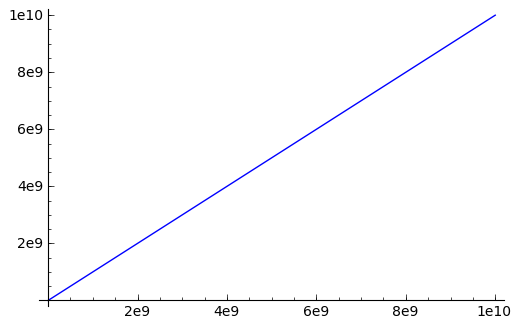
\includegraphics[height=4cm]{figures/x.png}}
	\hfill
	\subfloat[$10^x$]{\label{10hochx}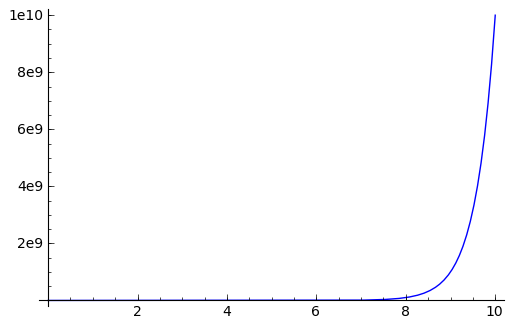
\includegraphics[height=4cm]{figures/10hochx.png}}
	\caption{Graph of the functions $x$ and $10^x$}
	\label{xund10hochx}
        \vskip +25pt 
\end{figure}


\subsubsection*{The function $\ln{x}$}
In comparison to that we consider the function $\ln{x}$. The left picture of figure \ref{lnxbis} on page \pageref{lnxbis} shows the graph with the domain of definition from $1$ to $100$. On the right picture the domain of definition was chosen between $1$ and $10^{10}$.\\
One can see that the values of the function $\ln{x}$ grow slowly compared to the growth of the function $x$. This is visualizd by the graph of both functions in one picture shown in figure \ref{xundlnxundxdurchlnx} on page \pageref{xundlnxundxdurchlnx}. In addition to that the graph of the function $\frac{x}{\ln{x}}$ was drawn in the same figure.

\begin{figure}[!htb]
	\centering
	\subfloat[ ]{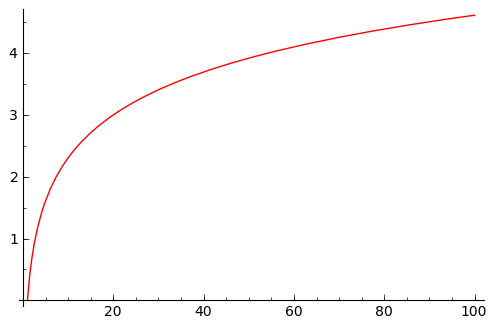
\includegraphics[height=4cm]{figures/lnxbis100.png}}
	\hfill
	\subfloat[ ]{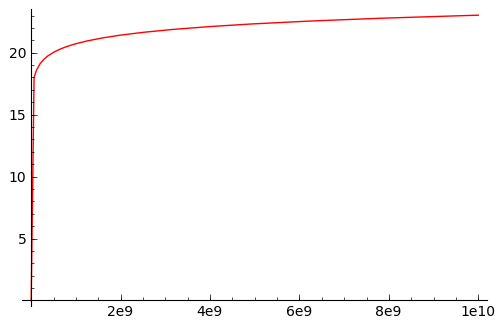
\includegraphics[height=4cm]{figures/lnxbis10hoch10.png}}
	\caption{Graph of the function $\ln{x}$ till $100$ and till $10^{10}$}
	\label{lnxbis}
        \vskip +25pt 
\end{figure}

\begin{figure}[!htb]
	\centering
	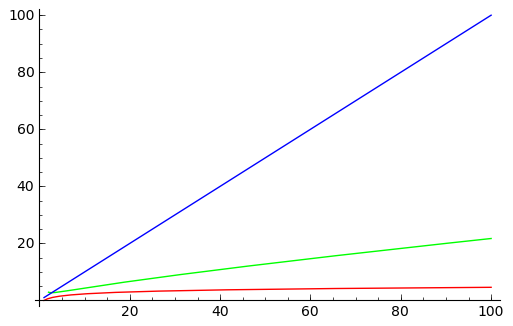
\includegraphics[height=4cm]{figures/xundlnxundxdurchlnx.png}
	\caption{The functions $x$ (blue), $\ln{x}$ (red)
                 and $\frac{x}{\ln{x}}$ (green)}
	\label{xundlnxundxdurchlnx}
        \vskip +25pt 
\end{figure}


\subsubsection*{The function $PI(x) = \frac{x}{\ln{x}}$}
\index{PI(x), $\Pi(x)$}
The function $\frac{x}{\ln{x}}$ consists of the function $x$ as the numerator and the function $\ln{x}$ in the denominator, which, in comparison to $x$, increases very slowly. Compared to the number $x$ itself, the number of primes less or equal to $x$ is small. But still, $\frac{x}{\ln{x}}$ is an increasing function as you can see in figure \ref{xundlnxundxdurchlnx} on page \pageref{xundlnxundxdurchlnx}.


\subsubsection*{The number of primes in the different intervals}
\label{primes:_Appendix_subsubsection_NumberofPrimes-in-intervals}
Figure \ref{deltazehnxdurchlnxbis}
% on page \pageref{deltazehnxdurchlnxbis}
visualizes how the number of primes in the intervals $[1, 10^x]$ and
$[10^{x-1},10^{x}]$ behave.
To calculate it faster, the result of the approximation function is used
(not the exact numbers like in the tables in chapter \ref{s:primhfk}).

Here for each base 10 exponent two bars are drawn:
$\frac{10^{x}}{\ln{10^{x}}}$ and $\frac{10^{x}}{\ln{10^{x}}}-\frac{10^{x-1}}{\ln{10^{x-1}}}$:
The left chart shows the values for the exponents $x$ from $1$ to $5$,
and the right one for $x$ from $1$ to $10$, where $x$ is the base 10 exponent.\\

The blue bars represent the overall number of primes up to $10^x$. The red bars show how many primes accrue in the interval $[10^{x-1},10^x]$, respectively.
This makes clear, that the number of primes in intervals of higher exponents keeps growing quite fast. 

\begin{figure}[!htb]
	\centering
	\subfloat[ ]{\label{deltazehnxdurchlnxbis5}
                     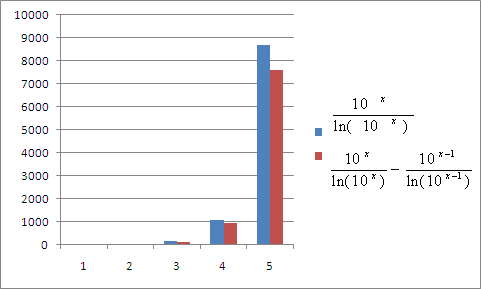
\includegraphics[height=4cm]{figures/deltazehnxdurchlnxbis5.png}}
	\hfill
	\subfloat[ ]{\label{deltazehnxdurchlnxbis10}
                     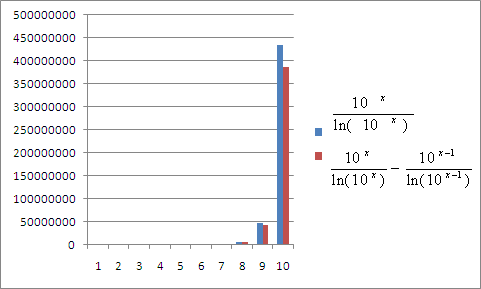
\includegraphics[height=4cm]{figures/deltazehnxdurchlnxbis10.png}}
	\caption{Numbers of primes in the interval $[1, 10^x]$ (blue) and in the
        interval $[10^{x-1},10^x]$ (red) for different exponents $x$}
	\label{deltazehnxdurchlnxbis}
\end{figure}


A table containing the number of primes in some dedicated intervals can be found
in chapter \ref{s:primhfk} at page \pageref{s:primhfk}:
For example, within the interval $[1, 10^4]$ there are 1229 primes;
thereof are in the interval $[10^3, 10^4]$ 1229 - 168 = 1061 primes.

Theory about the prime number theorem and the function PI(x) can be found in
chapter \ref{l_Primes_Distrib-of-Primes}.




\begin{sagecode}
\begin{Verbatim}%
[fontsize=\footnotesize,fontshape=tt]

# Definition of function f(x)=x and plots for the domains from 0 to 10^10 and 0 to 100
sage: def f(x):return x
....:
sage: F=plot(f,(0,10^10))
sage: F.plot()

sage: F2=plot(f,(1,100))
sage: F2.plot()


# Definition of function g(x)=10^x and plots for the domain from 0 to 10
sage: def g(x): return 10^x
....:
sage: G=plot(g,(0,10))
sage: G.plot()


# Definition of function h(x)=log(x) and plots for the domains from 1 to 100 and 1 to 10^10
sage: def h(x): return log(x)
....:
sage: H=plot(h,(1,100),color="red")
sage: H.plot()

sage: H2=plot(h,(1,10^10),color="red")
sage: H2.plot()


# Definition of function k(x)=x/log(x) and plots for the domain from 2 to 100
sage: def k(x): return x/log(x)
....:
sage: K=plot(k,(2,100),color="green")
sage: K.plot()


# Plots of the functions f, k and h for the domain of definition up to 100
sage: F2+K+H


# Generation of the data for the bar charts ..........................
# Determination of the number of primes in the interval [1,10]
sage: pari(10).primepi()-pari(1).primepi()
4

# Determination of the number of primes in the interval [10^3,10^4]
sage: pari(10**4).primepi()-pari(10**3).primepi()
1061

# Determination of the number of primes in the interval [10^8,10^9]
sage: pari(10**9).primepi()-pari(10**8).primepi()
45086079

# (for 10^10: OverflowError: long int too large to convert)

\end{Verbatim}
\caption{Generation of the graphs of the three functions x, log(x) and x/log(x)}
\end{sagecode}



% ---------------------------------------------------------------------------
% ---------------------------------------------------------------------------
\clearpage
\newpage
\hypertarget{primes:_Appendix_Sage-Samples}{}
\section{Appendix: Examples using Sage}
% \section*{Appendix A: Examples using Sage}
% \addcontentsline{toc}{section}{Appendix A: Examples using Sage}
\label{primes:_Appendix_Sage-Samples}
\index{Sage!Code examples}
\index{Sage}

\noindent Below is Sage source code related to contents of the
chapter~\ref{Label_Kapitel_Primes} (``\nameref{Label_Kapitel_Primes}''). 


% ---------------------------------------------------------------------------
% \newpage
\subsection{Some basic functions about primes using Sage}
\index{Sage}

This part of the appendix contains Sage code, to perform some simple
computations about primes.%
\footnote{See the Sage documentation about Elementary number theory
          \url{http://www.sagemath.org/doc/constructions/number_theory.html}.}

\begin{sagecode}
\begin{Verbatim}%
[fontsize=\footnotesize,fontshape=tt]

# primes (general commands)
# The set of prime numbers
sage: P=Primes(); P
Set of all prime numbers: 2, 3, 5, 7, ...

# Returns the next prime number
sage: next_prime(5)
7

# Returns how many primes <=x are there
sage: pari(10).primepi()
4

# Returns the first x primes
sage: primes_first_n(5)
[2, 3, 5, 7, 11]

# Returns the primes in an interval
sage: list(primes(1,10))
[2, 3, 5, 7]

\end{Verbatim}
\caption{Some basic functions about primes}
\end{sagecode}



% ---------------------------------------------------------------------------
\newpage
\subsection{Check primality of integers generated by quadratic functions}
\index{Sage}

The following Sage code verifies the primality of integers generated
by the function $f(n) = n^2 - 9n + 61$.
The code defines a function called \verb!quadratic_prime_formula()!
that takes three arguments:
\begin{itemize}
\item \verb!start! --- An integer which is the lower bound for
  integers in the sequence $\texttt{start}, \texttt{start} + 1,
  \texttt{start} + 2, \dots, \texttt{end} - 1, \texttt{end}$.

\item \verb!end! --- An integer which is the upper bound for the
  integers in the sequence $\texttt{start}, \texttt{start} + 1,
  \texttt{start} + 2, \dots, \texttt{end} - 1, \texttt{end}$.

\item \verb!verbose! --- (default: \verb!True!) a flag to signify
  whether to print a message indicating the primality of an integer
  generated by $f(n)$.
\end{itemize}

\noindent A meaningful modification of this code is to use another function, of
which the primality of its function values should be checked.


\begin{sagecode}
\begin{Verbatim}%
[fontsize=\footnotesize,fontshape=tt]
def quadratic_prime_formula(start, end, verbose=True):
    print "N -- N^2 - 9*N + 61"
    P = 0 # the number of primes between start and end
    for n in xrange(start, end + 1):
        X = n^2 - 9*n + 61
        if is_prime(X):
            P += 1
            if verbose:
                 print str(n) + " -- " + str(X) + " is prime"
        else:
            if verbose:
                 print str(n) + " -- " + str(X) + " is NOT prime"
    print "Number of primes: " + str(P)
    print "Percentage of primes: " + str(float((P * 100) / (end - start + 1)))
\end{Verbatim}
\caption{Verify the primality of integers generated by a quadratic function}
\end{sagecode}

\vspace{12pt}
With the following function call we compute the values of $f(n) = n^2 - 9n + 61$ for
$n = 0, 1, 2, \dots, 50$ and verify the primality of the generated integers:

\begin{Verbatim}%
[fontsize=\footnotesize,fontshape=tt]
sage: quadratic_prime_formula(0, 50)
 N -- N^2 - 9*N + 61
0 -- 61 is prime
1 -- 53 is prime
2 -- 47 is prime
3 -- 43 is prime
4 -- 41 is prime
5 -- 41 is prime
6 -- 43 is prime
7 -- 47 is prime
8 -- 53 is prime
9 -- 61 is prime
10 -- 71 is prime
11 -- 83 is prime
12 -- 97 is prime
13 -- 113 is prime
14 -- 131 is prime
15 -- 151 is prime
16 -- 173 is prime
17 -- 197 is prime
18 -- 223 is prime
19 -- 251 is prime
20 -- 281 is prime
21 -- 313 is prime
22 -- 347 is prime
23 -- 383 is prime
24 -- 421 is prime
25 -- 461 is prime
26 -- 503 is prime
27 -- 547 is prime
28 -- 593 is prime
29 -- 641 is prime
30 -- 691 is prime
31 -- 743 is prime
32 -- 797 is prime
33 -- 853 is prime
34 -- 911 is prime
35 -- 971 is prime
36 -- 1033 is prime
37 -- 1097 is prime
38 -- 1163 is prime
39 -- 1231 is prime
40 -- 1301 is prime
41 -- 1373 is prime
42 -- 1447 is prime
43 -- 1523 is prime
44 -- 1601 is prime
45 -- 1681 is NOT prime
46 -- 1763 is NOT prime
47 -- 1847 is prime
48 -- 1933 is prime
49 -- 2021 is NOT prime
50 -- 2111 is prime
Number of primes: 48
Percentage of primes: 94.1176470588
\end{Verbatim}

\noindent The last two lines of the output contain a small statistics.
You can see that $f(n)$ generates
48 primes when $0 \leq n \leq 50$, which is approximately 94\% of the
values generated by $f(n)$.\\

For larger sequences, it is impractical to print all single messages indicating
the primality of integers. In the following Sage session, only the statistics at
the end is printed (by setting the verbose parameter to false): the overall
number of primes and the percentage of primes, generated by $f(n)$ where
$0 \leq n \leq 1000$.

\begin{Verbatim}%
[fontsize=\footnotesize,fontshape=tt]
sage: quadratic_prime_formula(0, 1000, False)
N -- N^2 - 9*N + 61
Number of primes: 584
Percentage of primes: 58.3416583417
\end{Verbatim}








% --------------------------------------------------------------------------
\newpage
\begin{thebibliography}{99999}
\addcontentsline{toc}{section}{Bibliography}


\bibitem[Aaronson2003]{pr:Aaronson2003} \index{Aaronson 2003}
    Scott Aaronson, \\
    {\em The Prime Facts: From Euclid to AKS}, \\
    \url{http://www.scottaaronson.com/writings/prime.pdf} \\
    After I had completed the first edition of this article, I did come
    across the fine paper by Scott Aaronson, which also offers
    a didactically very well-done introduction to this topic. It is 
    humorous and easy to read but at the same time precise and erudite.

% already defined in elementaryNumberTheory.inc -> 2 davor
\bibitem[Bartholome1996]{pr:2Bartholome1996}  \index{Bartholome 1996}
    A. Bartholom\'e, J. Rung, H. Kern, \\     
    {\em Zahlentheorie f\"ur Einsteiger}, Vieweg, 1995, 2nd edition 1996.

\bibitem[Blum1999]{pr:Blum1999} \index{Blum 1999}   
    W. Blum, \\     
    {\em Die Grammatik der Logik}, dtv, 1999.

\bibitem[Bundschuh1998]{pr:Bundschuh1998} \index{Bundschuh 1998}
    Peter Bundschuh, \\
    {\em Einf\"uhrung in die Zahlentheorie}, Springer, 1988, 4th edition 1998.

\bibitem[Crandell2001]{pr:Crandell2001} \index{Crandell 2001} \index{Pomerance 2001}
    Richard Crandell, Carl Pomerance, \\
    {\em Prime Numbers. A Computational Perspective}, Springer, 2001.

\bibitem[Doxiadis2000]{pr:Dioxadis2000}
    Apostolos Doxiadis, \\
    {\em Uncle Petros and the Goldbach's Conjecture}, \\
    Faber/Bloomsbury, 2000.

\bibitem[Graham1989]{pr:Graham1989} \index{Graham 1989}     
   R.E. Graham, D.E. Knuth, O. Patashnik, \\
   {\em Concrete Mathematics}, Addison-Wesley, 1989.

\bibitem[Klee1997]{pr:Klee1997} \index{Klee 1997}     
   V. Klee, S. Wagon, \\
   {\em Ungel\"oste Probleme in der Zahlentheorie und der Geometrie der 
   Ebene}, \\ Birkh\"auser Verlag, 1997.

\bibitem[Knuth1981]{pr:Knuth1981} \index{Knuth 1981}     
   Donald E. Knuth, \\ 
   {\em The Art of Computer Programming, vol 2: Seminumerical Algorithms}, \\
   Addison-Wesley, 1969, 2nd edition 1981.

\bibitem[Lorenz1993]{pr:Lorenz1993} \index{Lorenz 1993}     
   F. Lorenz, \\
   {\em Algebraische Zahlentheorie}, BI Wissenschaftsverlag, 1993.

\bibitem[Oppliger2011]{pr:Oppliger2011} \index{Oppliger 2011}
    Rolf Oppliger \\
    {\em Contemporary Cryptography, Second Edition},
    Artech House, 2011, \\
    \url{http://books.esecurity.ch/cryptography2e.html}.

\bibitem[Padberg1996]{pr:Padberg1996} \index{Padberg 1996}     
   Friedhelm Padberg, \\
   {\em Elementare Zahlentheorie}, 
   Spektrum Akademischer Verlag, 1988, 2nd edition 1996.

\bibitem[Pieper1983]{pr:Pieper1983} \index{Pieper 1983}     
   H. Pieper, \\
   {\em Zahlen aus Primzahlen}, 
   Verlag Harri Deutsch, 1974, 3rd edition 1983.

\bibitem[Rempe2009]{pr:Rempe2009}  \index{Rempe 2009}
    L. Rempe, R. Waldecker, \\
    {\em Primzahltests f\"ur Einsteiger}, Vieweg+Teubner, 2009. \\
    This books results from a course for specially talented pupils at the
    ``Deutsche Sch\"ulerakademie''.
    It completely presents the AKS proof -- without expecting mathematical
    pre-knowledge.

\bibitem[Richstein1999]{pr:Richstein1999} \index{Richstein 1999}
    J. Richstein, \\
    {\em Verifying the Goldbach Conjecture up to $4*10^{14},$}
    Mathematics of Computation 70, 2001, p. 1745-1749). 

\bibitem[Scheid1994]{pr:Scheid1994} \index{Scheid 1994}
    Harald Scheid, \\ 
    {\em Zahlentheorie}, BI Wissenschaftsverlag, 2nd edition 1994.

\bibitem[Schneier1996]{pr:Schneier1996p} \index{Schneier 1996}     
    Bruce Schneier, \\
    {\em Applied Cryptography, Protocols, Algorithms, and Source Code in C},\\
    Wiley and Sons, 2nd edition 1996.

\bibitem[Schroeder1999]{pr:Schroeder1999} \index{Schroeder 1999}
    M.R. Schroeder, \\
    {\em Number Theory in Science and Communication}, \\ 
    Springer, 1984, 3rd edition 1997, Corrected Printing 1999.

\bibitem[Schwenk1996]{pr:Schwenk1996} \index{Schwenk 1996}     
    J. Schwenk \\
    {\em Conditional Access}, 
    in taschenbuch der telekom praxis, 1996, \\
    Hrgb. B. Seiler, Verlag Schiele und Sch\"on, Berlin.

\bibitem[Shoup2005]{pr:Shoup2005} \index{Shoup 2005}
    Victor Shoup \\
    {\em A Computational Introduction to Number Theory and Algebra},\\
    Cambridge University Press, 2005, \\
    \url{http://shoup.net/ntb/}.

\bibitem[Tietze1973]{pr:Tietze1973} \index{Tietze 1973}     
    H. Tietze, \\
    {\em Gel\"oste und ungel\"oste mathematische Probleme}, \\
    Verlag C. H. Beck, 1959, 6th edition 1973.

\end{thebibliography}


% --------------------------------------------------------------------------
\newpage
% \section*{Web links} \addcontentsline{toc}{section}{Web links}
\chapter*{Web links} \addcontentsline{toc}{section}{Web links}

\begin{enumerate}
\item GIMPS (Great Internet Mersenne-Prime Search) 
      \index{Mersenne!prime number}  \index{GIMPS} \\
      www.mersenne.org is the home page of the GIMPS project, \\
      \url{http://www.mersenne.org/prime.htm}

\item The Proth Search Page with the Windows program by Yves Gallot \\
      \url{http://www.utm.edu/research/primes/programs/gallot/index.html}

\item Generalized Fermat Prime Search \\
      \url{http://primes.utm.edu/top20/page.php?id=12}

\item Distributed Search for Fermat Number Divisors \\
      \url{http://www.fermatsearch.org/}

\item At the University of Tennessee you will find extensive research
      results about prime numbers. \\
      \url{http://www.utm.edu/}

\item The best overview about prime numbers is offered from my point of view 
      by ~``The Prime Pages'' from professor Chris Caldwell.
      \index{Caldwell Chris} \\
      \url{http://www.utm.edu/research/primes}

\item Descriptions e.g.\ about prime number tests \\
      \url{http://www.utm.edu/research/primes/mersenne.shtml} \\
      \url{http://www.utm.edu/research/primes/prove/index.html}

\item Showing the $n$-th prime number P(n)\\
      \url{http://www.utm.edu/research/primes/notes/by_year.html}

\item The supercomputer manufacturer SGI Cray Research not only 
      employed brilliant mathematicians but also used the prime 
      number tests as benchmarks for its machines. \\
      \url{http://www.isthe.com/chongo/tech/math/prime/prime_press.html}
	 
\item The Cunningham Project, \index{Cunningham project}\\ 
      \url{http://www.cerias.purdue.edu/homes/ssw/cun/}

\item \url{http://www.eff.org/awards/coop}

% \item \url{http://www.informatik.tu-darmstadt.de/TI/LiDIA/}

\item \url{http://www.math.Princeton.EDU/~arbooker/nthprime.html}
% {\tt http://www.math.Princeton.EDU/\~{}arbooker/nthprime.html }

\item Goldbach conjecture verification project von Tom�s Oliveira e Silva,
      \index{Goldbach project}\\ 
      \url{http://www.ieeta.pt/~tos/goldbach.html}

\item \url{http://www.mathematik.ch/mathematiker/goedel.html}

\end{enumerate}




\vskip +10 pt
% --------------------------------------------------------------------------
\section*{Acknowledgments}
\addcontentsline{toc}{section}{Acknowledgments}

I would like to take this opportunity to thank Mr.\ Henrik Koy and Mr.\ Roger
Oyono for their very constructive proof-reading of the first versions
of this article.



% Local Variables:
% TeX-master: "../script-en.tex"
% End:

% $Id$
%\def\QM {{,\kern -0.9 pt ,}}
\setcounter{satz}{0}
\setcounter{definition}{0}

% ..........................................................................
% --------------------------------------------------------------------------
% ++++++++++++++++++++++++++++++++++++++++++++++++++++++++++++++++++++++++++
%              E l e m e n t a r e  Z a h l e n t h e o r i e
% /~~~~~~~~~~~~~~~~~~~~~~~~~~~~~~~~~~~~~~~~~~~~~~~~~~~~~~~~~~~~~~~~~~~~~~~~~

\hypertarget{Chapter_ElementaryNT}{}
\chapter{Einf�hrung in die elementare Zahlentheorie mit Beispielen}
\label{Chapter_ElementaryNT}
(Bernhard Esslinger, Juli 2001; Updates: Nov. 2001, Juni 2002, Mai 2003,
 Mai 2005, M�rz 2006, Juni 2007, Juli 2009) \\

Diese \glqq Einf�hrung\grqq~ bietet einen Einstieg f�r mathematisch Interessierte.
Erforderlich sind nicht mehr Vorkenntnisse als die, die im Grundkurs Mathematik am Gymnasium vermittelt werden.\par
Wir haben uns bewusst an \glqq Einsteigern\grqq~ und \glqq Interessenten\grqq~ orientiert, und nicht an den
Gepflogenheiten mathematischer Lehrb�cher, die auch dann \glqq Einf�hrung\grqq~ genannt werden,
wenn sie schon auf der 5. Seite nicht mehr auf Anhieb zu verstehen sind und sie eigentlich den Zweck haben, dass
man danach auch spezielle Monographien zu dem Thema lesen k�nnen soll.



% ++++++++++++++++++++++++++++++++++++++++++++++++++++++++++++++++++++++++++
\section{Mathematik und Kryptographie}
Ein gro�er Teil der modernen, asymmetrischen Kryptographie beruht auf 
mathematischen Erkenntnissen -- auf den Eigenschaften (\glqq Gesetzen'')
ganzer Zahlen, die in der elementaren \index{Zahlentheorie!elementare}
Zahlentheorie untersucht werden. \glqq Elementar\grqq\ bedeutet hier, 
dass die zahlentheoretischen Fragestellungen im wesentlichen
in der Menge der nat�rlichen und der ganzen Zahlen durchgef�hrt werden.

Weitere mathematische Disziplinen, die heute in der Kryptographie 
Verwendung finden, sind 
(vgl. \cite[S. 2]{nt:Bauer1995}, \cite[Seite 3]{nt:Bauer2000}) :
\begin{itemize}
    \item Gruppentheorie
    \item Kombinatorik
    \item Komplexit�tstheorie
    \item Ergodentheorie
    \item Informationstheorie.
\end{itemize}

Die Zahlentheorie oder Arithmetik (hier wird mehr der Aspekt des Rechnens
mit Zahlen betont) wurde von Carl Friedrich Gauss\footnote{%
  Carl Friedrich Gauss, deutscher Mathematiker und Astronom,
  30.4.1777$-$23.2.1855.
}
\index{Gauss, Carl Friedrich}
als besondere mathematische Disziplin begr�ndet. Zu ihren elementaren
Gegenst�nden geh�ren: gr��ter gemeinsamer Teiler\footnote{%
Auf ggT\index{ggT}, englisch gcd (greatest common divisor), geht dieser
Artikel in Anhang~\ref{NumberTheory_Appendix_GCD} ein.
} (ggT), Kongruenzen (Restklassen), Faktorisierung, Satz von Euler-Fermat und
primitive Wurzeln. Kernbegriff sind jedoch die Primzahlen und ihre
multiplikative Verkn�pfung.

Lange Zeit galt gerade die Zahlentheorie als Forschung pur, als
Paradebeispiel f�r die Forschung im Elfenbeinturm. Sie erforschte die
\glqq geheimnisvollen Gesetze im Reich der Zahlen'' und gab Anlass zu
philosophischen Er�rterungen, ob sie beschreibt, was �berall in der Natur
schon da ist, oder ob sie ihre Elemente (Zahlen, Operatoren, Eigenschaften)
nicht k�nstlich konstruiert.

Inzwischen wei� man, dass sich zahlentheoretische Muster �berall in der Natur
finden. Zum Beispiel verhalten sich die Anzahl der links- und der
rechtsdrehenden Spiralen einer Sonnenblume zueinander wie zwei
aufeinanderfolgende\index{Fibonacci} Fibonacci-Zahlen\footnote{%
Die Folge der Fibonacci-Zahlen $(a_i)_{i \in \mathbb{N}}$ ist definiert durch die \glqq rekursive'' 
Vorschrift $a_1 := a_2 := 1$ und f�r alle Zahlen  $n=1,2,3,\cdots$ definiert man 
$a_{n+2} := a_{n+1}+a_n$.  Zu dieser historischen Folge gibt es viele interessante 
Anwendungen in der Natur (siehe z.B. \cite[S. 290 ff]{nt:Graham1994}\index{Graham 1994} oder die Web-Seite 
von \hyperlink{knott}{Ron Knott:} \index{Knott, Ron} hier dreht sich alles um Fibonacci-Zahlen). 
Die Fibonacci-Folge\index{Fibonacci} ist gut verstanden und wird heute als wichtiges Werkzeug in der 
Mathematik benutzt.
}, also z.B.  wie  $21 : 34$.

Au�erdem wurde sp�testens mit den zahlentheoretischen Anwendungen der
modernen Kryptographie klar, dass eine jahrhundertelang als theoretisch
geltende Disziplin praktische Anwendung findet, nach deren Experten heute
eine hohe Nachfrage auf dem Arbeitsmarkt besteht.

Anwendungen der (Computer-)Sicherheit bedienen sich heute der Kryptographie,
weil Kryptographie als mathematische Disziplin einfach besser und
beweisbarer ist als alle im Laufe der Jahrhunderte erfundenen \glqq kreativen''
Verfahren der Substitution und besser als alle ausgefeilten physischen
Techniken wie beispielsweise beim Banknotendruck \cite[S. 4]{nt:Beutelspacher1996}.

In diesem Artikel werden in einer leicht verst�ndlichen Art die
grundlegenden Erkenntnisse der elementaren Zahlentheorie anhand vieler
Beispiele vorgestellt -- auf Beweise wird (fast) vollst�ndig verzichtet
(diese finden sich in den mathematischen Lehrb�chern).

Ziel ist nicht die umfassende Darstellung der zahlentheoretischen Erkenntnisse,
sondern das Aufzeigen der wesentlichen Vorgehensweisen. Der Umfang des Stoffes
orientiert sich daran, das RSA-Verfahren\index{RSA} verstehen und anwenden
zu k�nnen.

Dazu wird sowohl an Beispielen als auch in der Theorie erkl�rt, wie man in
endlichen Mengen rechnet und wie dies in der Kryptographie Anwendung findet.
Insbesondere wird auf die klassischen Public-Key-Verfahren Diffie-Hellman
\index{Diffie-Hellman} (DH) und RSA\index{RSA} eingegangen.

Au�erdem war es mir wichtig, fundierte Aussagen zur Sicherheit des RSA-Verfahrens zu machen.



\vskip +40 pt

\begin{center}
\fbox{\parbox{15cm}{{\em Carl Friedrich Gauss:\index{Gauss, Carl Friedrich}}\\
Die Mathematik ist die K�nigin der Wissenschaften, die Zahlentheorie aber
ist die K�nigin der Mathematik.}}
\end{center}

% ++++++++++++++++++++++++++++++++++++++++++++++++++++++++++++++++++++++++++
\section{Einf�hrung in die Zahlentheorie}
\index{Zahlentheorie!Einf�hrung} 

Die Zahlentheorie entstand aus Interesse an den positiven ganzen Zahlen $1,
2, 3, 4, \cdots ,$ die auch als die Menge der \index{Zahlen!nat�rliche}
{\em nat�rlichen Zahlen} $\mathbb{N}$ bezeichnet
werden. Sie sind die ersten mathematischen Konstrukte der menschlichen
Zivilisation. Nach Kronecker\footnote{%
Leopold Kronecker, deutscher Mathematiker, 7.12.1823$-$29.12.1891.
}
\index{Kronecker, Leopold} hat sie der liebe Gott geschaffen, 
nach Dedekind\footnote{Julius Wilhelm Richard Dedekind,
deutscher Mathematiker, 06.10.1831$-$12.02.1916.
}
\index{Dedekind, Julius} der menschliche Geist.
Das ist je nach Weltanschauung ein unl�sbarer Widerspruch oder
ein und dasselbe.

Im Altertum gab es keinen Unterschied zwischen Zahlentheorie und
Numerologie, die einzelnen Zahlen mystische Bedeutung zuma�. So wie sich
w�hrend der Renaissance (ab dem 14. Jahrhundert) die Astronomie allm�hlich
von der Astrologie und die Chemie von der Alchemie l�ste, so lie� auch die
Zahlentheorie die Numerologie hinter sich.

Die Zahlentheorie faszinierte schon immer Amateure wie auch professionelle
Mathematiker. Im Unterschied zu anderen Teilgebieten der Mathematik k�nnen
viele der Probleme und S�tze auch von Laien verstanden werden, andererseits
widersetzten sich die L�sungen zu den Problemen und die Beweise zu den S�tzen
oft sehr lange den Mathematikern. Es ist also leicht, gute Fragen zu stellen,
aber es ist ganz etwas anderes, die Antwort zu finden. Ein Beispiel daf�r ist
der sogenannte letzte (oder gro�e) Satz von Fermat\footnote{Thema der
   Schul-Mathematik ist der Satz von Pythagoras\index{Pythagoras!Satz von},
   wo gelehrt wird, dass in einem rechtwinkligen Dreieck gilt:
   $a^2 + b^2 = c^2$, wobei $a, b$ die Schenkell�ngen sind und 
   c die L�nge der Hypothenuse ist.
   Fermats ber�hmte Behauptung war, dass f�r $a,b,c \in \mathbb{N}$ und
   f�r ganzzahlige Exponenten $n > 2$ immer die Ungleichheit
   $a^n + b^n \not= c^n$ gilt.  Leider fand \index{Fermat!letzter Satz}
   Fermat auf dem Brief, wo er die Behauptung aufstellte, nicht gen�gend
   Platz, um den Satz zu beweisen. Der Satz konnte erst �ber 300 Jahre sp�ter
   bewiesen werden \cite[S. 433-551]{nt:Wiles1994}. \index{Wiles, Andrew}
}.

Bis zur Mitte des 20. Jahrhunderts wurde die Zahlentheorie als das reinste
Teilgebiet der Mathematik angesehen -- ohne Verwendung in der wirklichen Welt.
Mit dem Aufkommen der Computer und der digitalen Kommunikation �nderte sich
das: die Zahlentheorie konnte einige unerwartete Antworten f�r reale
Aufgabenstellungen liefern. Gleichzeitig halfen die Fortschritte in der EDV,
dass die Zahlentheoretiker gro�e Fortschritte machten im Faktorisieren gro�er
Zahlen, in der Bestimmung neuer Primzahlen, im Testen von (alten)
Vermutungen und beim L�sen bisher unl�sbarer numerischer Probleme.

Die moderne Zahlentheorie \index{Zahlentheorie!moderne} besteht aus Teilgebieten wie
\begin{itemize}
    \item Elementare Zahlentheorie
    \item Algebraische Zahlentheorie
    \item Analytische Zahlentheorie
    \item Geometrische Zahlentheorie
    \item Kombinatorische Zahlentheorie
    \item Numerische Zahlentheorie und
    \item Wahrscheinlichkeitstheorie.
\end{itemize}

Die verschiedenen Teilgebiete besch�ftigen sich alle mit Fragestellungen zu
den ganzen Zahlen (positive und negative ganze Zahlen und die Null), gehen
diese jedoch mit verschiedenen Methoden an.

Dieser Artikel besch�ftigt sich nur mit dem Teilgebiet der elementaren
Zahlentheorie.
\newpage


% --------------------------------------------------------------------------
\subsection{Konvention}
Wird nichts anderes gesagt, gilt: 
\begin{itemize}
\item Die Buchstaben $a, b, c, d, e, k, n, m, p, q$ stehen f�r ganze Zahlen.
\item Die Buchstaben $i$ ~\mbox{und} ~$j$ stehen f�r nat�rliche Zahlen. 
\item Der Buchstabe $p$ steht stets f�r eine Primzahl.
\item Die Mengen $\mathbb{N} = \{ 1, 2, 3, \cdots \}$ und $\mathbb{Z} =\{ \cdots, -3, -2, -1, 0, 1, 2, 3, \cdots \}$ 
sind die {\em nat�rlichen} und die {\em ganzen} Zahlen.
\end{itemize}



%\vskip +40 pt
\newpage

\begin{center}
\fbox{\parbox{15cm}{{\em Joanne K. Rowling\index{Rowling, Joanne}\footnotemark:}\newline Das ist nicht Zauberei, das ist Logik, ein R�tsel.
Viele von den gr��ten Zauberern haben keine Unze Logik im Kopf.}}
\end{center}
\addtocounter{footnote}{0}\footnotetext{Joanne K. Rowling,~\glqq Harry Potter und der Stein der Weisen'', Carlsen, (c)
1997, Kapitel ~\glqq Durch die Fallt�r'', S. 310, Hermine.}


% ++++++++++++++++++++++++++++++++++++++++++++++++++++++++++++++++++++++++++
\section{Primzahlen und der erste Hauptsatz der elementaren Zahlentheorie}
\index{Zahlentheorie!elementare} Viele der Probleme in der elementaren
Zahlentheorie besch�ftigen sich mit Primzahlen.

Jede ganze Zahl hat Teiler oder Faktoren. Die Zahl 1 hat nur einen, n�mlich
sich selbst. Die Zahl 12 hat die sechs Teiler 1, 2, 3, 4, 6 und 12\footnote{%
Aufgrund der gro�en Teilerzahl von 12 findet sich diese Zahl -- und Vielfache dieser Zahl -- oft im allt�glichen wieder:
Die 12 Stunden-Skala der Uhr, die 60 Minuten einer Stunde, die 360 Grad-Skala der Winkelmessung, usw. Teilt man 
diese Skalen in Bruchteile auf, so ergeben sich in vielen F�llen die Br�che als ganze Zahlen. Mit diesen kann 
man im Kopf einfacher rechnen als mit gebrochenen Zahlen.
}. Viele Zahlen sind nur teilbar durch sich selbst und durch 1. Bez�glich der
Multiplikation sind dies die \glqq Atome'' im Bereich der Zahlen.

\index{Primzahl}
\begin{definition}\label{def-zth-prime} 
{\bf Primzahlen} sind nat�rliche Zahlen gr��er als $1$, die nur durch $1$ und sich
selbst teilbar sind.
\end{definition}

Per Definition ist $1$ keine Primzahl.

Schreibt man die Primzahlen in aufsteigender Folge (Primzahlenfolge), so
ergibt sich
$$2,~ 3,~ 5,~ 7,~ 11, ~13,~ 17,~ 19, ~23, ~29, ~31, ~37,~ 41,~ 43,~ 47,~ 53, ~59, ~61, ~67, ~71,
~73, ~79, ~83, ~89, ~97, \cdots.$$

Unter den ersten $100$ Zahlen gibt es genau $25$ Primzahlen. Danach nimmt ihr
prozentualer Anteil ab, wird aber nie Null.

Primzahlen treten als ganze Zahlen nicht selten auf. Allein im letzten
Jahrzehnt waren drei Jahre prim: $1993, 1997$ und $1999$. W�ren sie selten,
k�nnte die Kryptographie auch nicht so mit ihnen arbeiten, wie sie es tut.

Primzahlen k�nnen nur auf eine einzige (\glqq triviale'') Weise zerlegt werden:
\begin{eqnarray*}
5 & = & 1 * 5 \nonumber \\
17 & =  & 1 * 17 \nonumber \\
1.013 &  = & 1 * 1013 \nonumber \\
1.296.409 & = & 1 * 1.296.409. \nonumber
\end{eqnarray*}

\index{Zahlen!zusammengesetzte}
\begin{definition}\label{def-zth-composite} 
Nat�rliche Zahlen gr��er $1$, die keine Primzahlen sind, hei�en
{\bf zusammengesetzte Zahlen}: Diese haben mindestens zwei von $1$ verschiedene
Faktoren.
\end{definition}


\begin{example}{ Primfaktorzerlegung\index{Primfaktor!Zerlegung} solcher Zahlen:}
\begin{eqnarray*}
4 & = & 2*2  \nonumber \\
6 & = & 2*3  \nonumber \\
91 & = & 7*13  \nonumber \\
161 & = & 7*23  \nonumber \\
767 & = & 13*59  \nonumber \\
1.029 & = & 3 * 7^3  \nonumber \\
5.324 & = & 22 * 11^3.  \nonumber 
\end{eqnarray*}

\begin{satz}\label{thm-zth-cnum}
Jede zusammengesetzte Zahl $a$ besitzt einen kleinsten Teiler gr��er
als $1$. Dieser Teiler ist eine Primzahl $p$ und kleiner oder gleich der Quadratwurzel
aus $a$.
\end{satz}
\end{example}
Aus den Primzahlen lassen sich alle ganzen Zahlen gr��er als $1$
zusammensetzen -- und das sogar in einer {\em eindeutigen} Weise.

Dies besagt \index{Zahlentheorie!Hauptsatz} der 1. {\em Hauptsatz der Zahlentheorie} (= Hauptsatz der elementaren
Zahlentheorie = fundamental theorem of arithmetic = fundamental building
block of all positive integers). Er wurde das erste Mal pr�zise von Carl
Friedrich Gauss in seinen Disquisitiones Arithmeticae (1801) formuliert. 
\index{Zahlentheorie!Hauptsatz}  \index{Gauss, Carl Friedrich}

\begin{satz}{\bf Gauss 1801}\label{thm-zth-mthm}
Jede nat�rliche Zahl $a$ gr��er als $1$ l�sst sich als Produkt von
Primzahlen schreiben. Sind zwei solche Zerlegungen $a = p_1*p_2*\cdots*p_n = q_1*q_2*\cdots*q_m$ gegeben, dann
gilt nach eventuellem Umsortieren $n = m$ und f�r alle $i$: $p_i = q_i$.
\end{satz}

In anderen Worten: Jede nat�rliche Zahl au�er der $1$ l�sst sich auf genau eine
Weise als Produkt von Primzahlen schreiben, wenn man von der Reihenfolge der
Faktoren absieht. Die Faktoren sind also eindeutig (die \glqq Expansion in
Faktoren'' ist eindeutig)!

Zum Beispiel ist $60 = 2*2*3*5 = 2^2*3*5$. Und das ist --- bis auf eine
ver�nderte Reihenfolge der Faktoren --- die einzige M�glichkeit, die Zahl $60$
in Primfaktoren\index{Primfaktor} zu zerlegen.

Wenn man nicht nur Primzahlen als Faktoren zul�sst, gibt es mehrere
M�glichkeiten der Zerlegung in Faktoren und die {\em Eindeutigkeit} (uniqueness)
geht verloren:
$$60 = 1*60 = 2*30 = 4*15 = 5*12 = 6*10 = 2*3*10 = 2*5*6 = 3*4*5 = \cdots$$
Der 1. Hauptsatz ist nur scheinbar selbstverst�ndlich. Man kann viele andere
Zahlenmengen\footnote{%
Diese Mengen werden speziell aus der Menge der nat�rlichen Zahlen gebildet.
Ein Beispiel findet sich in diesem \hyperlink{uniqueness}{Skript}
auf Seite~\pageref{thm-pz-euklid} %eigentlich \pageref{remFundTheoOfArithm},
%aber hyperref ist buggy
am Ende von Kapitel~\ref{primesinmath}.
}
konstruieren, bei denen eine multiplikative Zerlegung in die Primfaktoren
dieser Mengen {\em nicht} eindeutig ist.

F�r eine mathematische Aussage ist es deshalb nicht nur wichtig, f�r welche
Operation sie definiert wird, sondern auch auf welcher Grundmenge diese
Operation definiert wird.

Weitere Details zu den Primzahlen (z.B. wie der \glqq Kleine Satz von 
Fermat'' zum Testen von sehr gro�en Zahlen auf ihre Primzahleigenschaft
benutzt werden kann) finden sich in diesem Skript in dem Artikel �ber 
\hyperlink{Kapitel_2}{Primzahlen, Kapitel~\ref{Label_Kapitel_2}}.


% ++++++++++++++++++++++++++++++++++++++++++++++++++++++++++++++++++++++++++
\section[Teilbarkeit, Modulus und Restklassen]
           {Teilbarkeit, Modulus und Restklassen\footnotemark}
\footnotetext{%
    \index{ZT, Lernprogramm Zahlentheorie}%
    \index{Lernprogramm ZT}%
    Mit dem Lernprogramm {\bf ZT} k�nnen Sie das hier und im Folgekapitel
    vorgestellte Rechnen mit Kongruenzen spielerisch nachvollziehen
    (siehe Lern-Kapitel 2.1, Seiten 2-9/40).\\
    ZT k�nnen Sie in CrypTool\index{CrypTool} �ber das Men�
    {\bf Einzelverfahren \textbackslash{} Zahlentheorie
    interaktiv \textbackslash{} Lernprogramm f�r Zahlentheorie} aufrufen.
    Siehe Anhang~\ref{s:appendix-Learn-NT}.
}
\index{Modulus} \index{Teilbarkeit}
Werden ganze Zahlen addiert, subtrahiert oder multipliziert, ist das
Ergebnis stets wieder eine ganze Zahl.

Die Division zweier ganzer Zahlen ergibt nicht immer eine ganze Zahl. Wenn
man z.B. $158$ durch $10$ teilt, ist das Ergebnis die Dezimalzahl $15,8$.
Dies ist keine ganze Zahl!

Teilt man $158$ dagegen durch $2$, ist das Ergebnis $79$ eine ganze Zahl.
In der Zahlentheorie sagt man, $158$ ist {\em teilbar} durch $2$, aber nicht durch $10$.
Allgemein sagt man:

\begin{definition}\label{def-zth-divisibility} \index{Teilbarkeit}
Eine ganze Zahl $n$ ist {\bf teilbar} durch eine ganze Zahl $d$, wenn der Quotient $n/d$
eine ganze Zahl $c$ ist, so dass $n = c * d$.
\end{definition}

Die Zahl $n$ wird {\em Vielfaches} von $d$ genannt; $d$ wird {\em Teiler, Divisor} \index{Teiler} \index{Divisor} oder \index{Faktor} {\em Faktor} von $n$
genannt.

Mathematisch schreibt man das: $d | n$ (gelesen: \glqq  $d$ teilt $n$'').
Die Schreibweise $d \!\!\not| n$ bedeutet, dass $d$ die Zahl $n$ nicht teilt.

Also gilt in unserem obigen Beispiel: $10\!\!\not| 158$, aber $2 | 158$.


% --------------------------------------------------------------------------
\subsection{Die Modulo-Operation -- Rechnen mit Kongruenzen} \index{Kongruenz}

Bei Teilbarkeitsuntersuchungen kommt es nur auf die Reste der Division an:
Teilt man eine Zahl $n$ durch $m$, so benutzt man oft die folgende Schreibweise:
$$\frac{n}{m} = c + \frac{r}{m} ,$$
wobei $c$ eine ganze Zahl ist und $r$ eine Zahl mit den Werten $0,1,\cdots, m-1$.
Diese Schreibweise hei�t Division mit Rest. Dabei hei�t $c$ der ganzzahlige 
\glqq Quotient'' und $r$ der \glqq Rest'' der Division.

\begin{example}{:}
$$\frac{19}{7} = 2 + \frac{5}{7} \quad (m=7, c = 2, r = 5)$$
\end{example}
Was haben die Zahlen $5, 12, 19, 26, \cdots$ bei der Division durch $7$ gemeinsam?
Es ergibt sich immer der Rest $r = 5$.
Bei der Division durch $7$ sind nur die folgenden Reste m�glich:
$$r = 0, 1, 2, \cdots, 6.$$

Wir fassen bei der Division durch $7$ die Zahlen, die den gleichen Rest $r$
ergeben, in die \glqq Restklasse $r$ modulo $7$'' zusammen. Zwei Zahlen $a$ und $b$, die
zur gleichen Restklasse modulo $7$ geh�ren, bezeichnen wir als \glqq kongruent
modulo 7''. Oder ganz allgemein:

\begin{definition}\label{def-zth-remainder} \index{Restklasse}
Als {\bf Restklasse $r$ modulo $m$} bezeichnet man alle ganzen Zahlen $a$, die bei der Division 
durch $m$ denselben Rest $r$ haben.
\end{definition}
\newpage
\begin{example}{:}
\begin{itemize}
\item[] Restklasse $0$ modulo $4 = \{ x | x = 4*n; \; n \in \mathbb{Z} \} = \{ \dots, -16, -12, -8, -4, 0, 4, 8, 12, 16, \dots \}$
\item[] Restklasse $3$ modulo $4 = \{ x | x = 4*n + 3;\; n \in \mathbb{Z} \} = \{ \dots, -13, -9, -5, -1, 3, 7, 11, 15, \dots \}$
\end{itemize}
\end{example}
Da modulo $m$ nur die Reste $0, 1, 2, \cdots, m-1$ m�glich sind, rechnet die modulare Arithmetik in endlichen Mengen. 
Zu jedem Modul $m$ gibt es genau $m$ Restklassen.

\begin{definition}\label{def-zth-congruence} \index{Kongruenz}
Zwei Zahlen $a, b \in \mathbb{N}$  hei�en \index{restgleich}
{\bf restgleich oder kongruent bez�glich $m \in \mathbb{N}$}  genau dann, 
wenn beim Teilen durch $m$ der gleiche Rest bleibt.
\end{definition}

Man schreibt: $a \equiv b {\rm ~(mod~} m)$. Und sagt:  {\em $a$ ist kongruent $b$ modulo $m$}. Das bedeutet, 
dass $a$ und $b$ zur gleichen Restklasse geh�ren. Der Modul ist also der Teiler. Diese Schreibweise wurde von 
Gauss eingef�hrt. Gew�hnlich ist der Teiler positiv, aber $a$ und $b$ k�nnen auch beliebige ganze Zahlen sein.

\begin{example}{:}
\begin{itemize}
   \item[] $19 \equiv 12 {\rm ~(mod~} 7)$,         
           denn die Reste sind gleich:  $19 / 7 = 2$ Rest $5$  und  $12 / 7 = 1$ Rest $5$.
   \item[] $23103 \equiv 0 {\rm ~(mod~} 453)$, denn $23103 / 453 = 51$ Rest $0$  und  $0 / 453 = 0$ Rest $0$.
\end{itemize}
\end{example}

\begin{satz}\label{thm-zth-div}
$a \equiv b$ (mod $m$) gilt genau dann,  wenn die Differenz $(a - b)$ durch $m$ teilbar ist, also wenn 
ein $q\in \mathbf{Z}$ existiert mit $ (a-b)=q*m.$
\end{satz}
Diese beiden Aussagen sind also �quivalent.

Daraus ergibt sich: Wenn $m$ die Differenz teilt, gibt es eine ganze Zahl $q$, so dass gilt: $a = b + q*m$.
Alternativ zur Kongruenzschreibweise kann man auch die Teilbarkeitsschreibweise verwenden: $m | (a - b)$.

\begin{example}{ f�r �quivalente Aussagen:} \\
$35 \equiv 11$ (mod $3) \Longleftrightarrow  35 - 11 \equiv 0$ (mod $3)$, 
wobei $35 - 11 = 24$ sich ohne Rest durch $3$ teilen l�sst, w�hrend $35:3$ und $11:3$ beide den Rest $2$ ergeben.
\end{example}

\begin{remark}{:}\\
F�r die Summe $(a + b)$ gilt die obige �quivalenz nicht!
\end{remark}

\begin{example}{:}\\
$11 \equiv 2$ (mod $3$), also ist $11 - 2 = 9 \equiv 0$ (mod $3$); aber $11 + 2 = 13$ ist nicht durch $3$ teilbar.
\end{example}

Die Aussage von Satz~\ref{thm-zth-div} gilt f�r Summen nicht einmal in eine
Richtung. Richtig ist sie bei Summen nur f�r den Rest $0$ und nur in der
folgenden Richtung: Teilt ein Teiler beide Summanden ohne Rest, teilt er
auch die Summe ohne Rest.


Anwenden kann man die obige �quivalenz von Satz~\ref{thm-zth-div}, wenn man schnell und
geschickt f�r gro�e Zahlen entscheiden will, ob sie durch eine bestimmte
Zahl teilbar sind.

\newpage
\begin{example}{:} \\
Ist $69.993$ durch $7$ teilbar?\\
Da die Zahl in eine Differenz zerlegt werden kann, wo einfach zu ersehen
ist, dass jeder Operand durch $7$ teilbar ist, ist auch die Differenz durch $7$
teilbar: $69.993 = 70.000 - 7$.
\end{example}

Diese �berlegungen und Definitionen m�gen recht theoretisch erscheinen, sind
uns im Alltag aber so vertraut, dass wir die formale Vorgehensweise gar nicht
mehr wahrnehmen: Bei der Uhr werden die $24$ h eines Tages durch die Zahlen $1$,
$2, \cdots, 12$ repr�sentiert. Die Stunden nach $12:00$ mittags erh�lt man als
Reste einer Division durch 12. Wir wissen sofort, dass $2$ Uhr nachmittags
dasselbe wie $14:00$ ist.

Diese \glqq modulare'', also auf die Divisionsreste bezogene Arithmetik ist die
Basis der asymmetrischen Verschl�sselungsverfahren.
Kryptographische Berechnungen spielen sich also nicht wie das Schulrechnen
unter den reellen Zahlen ab, sondern unter Zeichenketten begrenzter L�nge,
das hei�t unter positiven ganzen Zahlen, die einen gewissen Wert nicht
�berschreiten d�rfen.
Aus diesem und anderen Gr�nden w�hlt man sich eine gro�e Zahl $m$ und \glqq rechnet
modulo $m$'', das hei�t, man ignoriert ganzzahlige Vielfache von $m$ und rechnet
statt mit einer Zahl nur mit dem Rest bei Division dieser Zahl durch $m$.
Dadurch bleiben alle Ergebnisse im Bereich von $0$ bis $m-1$.


% ++++++++++++++++++++++++++++++++++++++++++++++++++++++++++++++++++++++++++
\section{Rechnen in endlichen Mengen}

% --------------------------------------------------------------------------
\subsection{Gesetze beim modularen Rechnen}

Aus S�tzen der Algebra folgt, dass wesentliche Teile der �blichen
Rechenregeln beim �bergang zum modularen Rechnen �ber der Grundmenge $\mathbb{Z}$
erhalten bleiben: Die Addition ist nach wie vor kommutativ. Gleiches gilt f�r die
Multiplikation modulo $m$. Das Ergebnis einer Division\footnote{%
\label{ftn-res-divmodn}
Die Division modulo $m$\index{Division modulo $n$}
ist nur f�r Zahlen, die teilerfremd\index{Zahlen!teilerfremd (co-prime)}
zu $m$ sind, definiert, da andere Zahlen die gleiche Eigenschaft wie Null haben.
Vergleiche Fu�snote~\ref{ftn-mod6} in Kapitel~\ref{addmult}.
} ist kein Bruch, sondern eine ganze Zahl zwischen $0$ und $m-1$.

\noindent Es gelten die bekannten Gesetze:
\begin{itemize}
\item[\bf 1.] {\bf Assoziativgesetz:}\index{Assoziativgesetz} \\ 
    $((a+b) + c) {\rm ~(mod~ } m) \equiv  (a + (b+c)) {\rm ~(mod~ } m).$ \\
    $((a*b) * c) {\rm ~(mod~ } m) \equiv  (a * (b*c)) {\rm ~(mod~ } m).$
\item[\bf 2.] {\bf Kommutativgesetz:} \index{Kommutativgesetz}\\
    $(a+b) {\rm ~(mod~ } m) \equiv  (b+a) {\rm ~(mod~ } m).$ \\
     $(a*b) {\rm ~(mod~ } m) \equiv  (b*a) {\rm ~(mod~ } m).$
\end{itemize}
Assoziativgesetz und Kommutativgesetz gelten sowohl f�r die Addition als auch f�r die Multiplikation.
\begin{itemize}
\item[\bf 3.] {\bf Distributivgesetz:} \index{Distributivgesetz}\\
    $ (a * (b+c)) {\rm ~(mod~ } m) \equiv  (a*b + a*c) {\rm ~(mod~ } m).$ 
\item[\bf 4.] {\bf Reduzierbarkeit:} \index{Reduzierbarkeit} \\
    $(a+b) {\rm ~(mod~} m) \equiv  (a {\rm ~(mod~ } m) + b {\rm ~(mod~ } m)) {\rm ~(mod~} m).$ \\  
    $(a*b) {\rm ~(mod~} m) \equiv  (a {\rm ~(mod~ } m) * b {\rm ~(mod~ } m)) {\rm ~(mod~} m).$ \\
    Beim Addieren und Multiplizieren ist es gleichg�ltig, in welcher Reihenfolge die Modulo-Operation durchgef�hrt wird.
\end{itemize}
\begin{itemize}
\item[\bf 5.] {\bf Existenz einer Identit�t (neutrales Element):} \index{Identit�t}\\
    $(a + 0) {\rm ~(mod~ } m) \equiv  (0 + a) {\rm ~(mod~ } m) \equiv  a {\rm ~(mod~ } m).$  \\
    $(a * 1) {\rm ~(mod~ } m) \equiv  (1 * a) {\rm ~(mod~ } m) \equiv  a {\rm ~(mod~ } m).$
\item[\bf 6.] {\bf Existenz des inversen Elements:} \\
    F�r jedes ganzzahlige $a$ und $m$ gibt es eine ganze Zahl $-a$, so dass gilt: \\
    $(a + (-a)) {\rm ~(mod~}m) \equiv  0 {\rm ~(mod~ } m)$ \quad (additive Inverse). \index{Inverse!additive}\\
    F�r jedes $a$ ($a \not\equiv 0 {\rm ~(mod~ } p$) ) und $p$ prim gibt es eine ganze Zahl $a^{-1}$, so dass gilt: \\
    $(a * a^{-1}) {\rm ~(mod~ } p) \equiv 1 {\rm ~(mod~}p)$ \quad (multiplikative Inverse). \index{Inverse!multiplikative}
\item[\bf 7.] \index{Abgeschlossenheit} {\bf Abgeschlossenheit:}\footnote{%
\label{ftn-closed}Diese Eigenschaft wird innerhalb einer Menge immer bez�glich einer Operation definiert. 
Siehe \hyperlink{NumberTheory_Appendix_B}{Anhang B zu diesem Kapitel}.
} \\
$a, b \in G  \Longrightarrow  ( a + b ) \in G.$ \\
$a, b \in G  \Longrightarrow  ( a * b ) \in G.$
\item[\bf 8.] \index{Transitivit�t} {\bf Transitivit�t:}\\
$ [ a \equiv b {\rm ~mod~ } m, ~b \equiv c {\rm ~mod~ } m] \Longrightarrow [ a \equiv c {\rm ~mod~ } m].
$
\end{itemize}


% --------------------------------------------------------------------------
\hypertarget{Chapter_ElementaryNT_5_2}{}
\subsection{Muster und Strukturen} \index{Struktur}
\label{Label_Chapter_ElementaryNT_5_2}

Generell untersuchen die Mathematiker \glqq Strukturen\grqq. Sie fragen sich
z.B. bei $ a * x \equiv b {\rm ~mod~ } m, $ welche Werte $x$ f�r gegebene 
Werte $a,b,m$ annehmen kann.

Insbesondere wird dies untersucht f�r den Fall, dass das Ergebnis $b$ der 
Operation das neutrale Element ist. Dann ist $x$ die Inverse von $a$ 
bez�glich dieser Operation.




\newpage
\begin{center}
\fbox{\parbox{15cm}{
    \emph{Seneca\index{Seneca}\footnotemark:}\\
    Lang ist der Weg durch Lehren, kurz und wirksam durch Beispiele.
}}
\end{center}
\addtocounter{footnote}{0}
\footnotetext{Lucius Annaeus Seneca, philosophischer Schriftsteller und
              Dichter, 4~v.~Chr. $-$ 65~n.~Chr.}

% ++++++++++++++++++++++++++++++++++++++++++++++++++++++++++++++++++++++++++
% \pagebreak
\section{Beispiele f�r modulares Rechnen}

Wir haben bisher gesehen:

F�r zwei nat�rliche Zahlen $a$ und $m$ bezeichnet  $a$ mod $m$  den Rest, den man erh�lt, 
wenn man $a$ durch $m$ teilt. Daher ist $a {\rm ~(mod~ } m$) stets eine Zahl zwischen $0$ und $m-1$.

Zum Beispiel gilt: $1 \equiv  6  \equiv  41 {\rm ~(mod~ } 5)$, denn der Rest ist jeweils $1$.

Ein anderes Beispiel ist: $2000  \equiv  0 {\rm ~(mod~ } 4)$, denn $4$ geht in $2000$ ohne Rest auf.

In der modularen Arithmetik gibt es nur eine eingeschr�nkte Menge
nicht-negativer Zahlen. Deren Anzahl wird durch einen Modul $m$ vorgegeben.
Ist der Modul $m = 5$, werden nur die 5 Zahlen der Menge $\{ 0, 1, 2, 3, 4\}$ benutzt.

Ein Rechenergebnis gr��er als $4$ wird dann \glqq modulo'' $5$ umgeformt, d.h. es ist
der Rest, der sich bei der Division des Ergebnisses durch $5$ ergibt. So ist
etwa $2*4 \equiv 8 \equiv 3 {\rm ~(mod~ } 5)$, da $3$ der Rest ist, wenn man $8$ durch $5$ teilt.


% --------------------------------------------------------------------------
\subsection{Addition und Multiplikation} \index{Addition} \index{Multiplikation}
\label{addmult}

Im folgenden werden 
\begin{itemize}
\item die Additionstabelle\footnote{%
Bemerkung zur Subtraktion modulo 5: \\
      $2 - 4 = -2 \equiv 3{\rm ~mod~}5.$\\
      Es gilt modulo $5$ also nicht, dass $-2 = 2$ (siehe auch \hyperlink{NumberTheory_Appendix_C}{Anhang C zu diesem Kapitel}). 
      } f�r ${\rm mod~ } 5$ (Tabelle~\ref{addmod5}) und
\item die Multiplikationstabellen\footnote{\label{ftn-mod6}%
Bemerkung zur Division modulo 6:\index{Division modulo $n$}

\noindent Bei der Division darf nicht durch die Null geteilt werden, dies liegt an
der besonderen Rolle der $0$ als Identit�t bei der Addition:\\
F�r alle $a$ gilt $a*0=0, $ denn $a*0 = a*(0+0) =a*0 + a*0.$ Es ist
offensichtlich, dass $0$ keine Inverse bzgl. der Multiplikation besitzt,
denn sonst m�sste gelten: $0 = 0 * 0^{-1} = 1.$ Vergleiche Fu�note
\ref{ftn-res-divmodn}.  } f�r mod $5$ (Tabelle~\ref{mulmod5}) und f�r mod $6$ (Tabelle~\ref{mulmod6})
\end{itemize}
aufgestellt.

% --------------------------------------------------------------------------
\begin{example}{ Additionstabelle:}\\
Das Ergebnis der Addition von $3$ und $4 {\rm ~(mod~ } 5)$ wird folgenderma�en bestimmt:
berechne $3 + 4 = 7$ und ziehe solange die $5$ vom Ergebnis ab, bis sich ein
Ergebnis kleiner als der Modul ergibt: $7 - 5 = 2$. Also ist: $3 + 4 \equiv 2 {\rm ~(mod~ } 5)$. 

\begin{table}[!ht]
\begin{center}
\begin{tabular}{r|ccccc}
+ &  0 & 1 & 2 & 3 & 4  \\
\hline
0 &  0 & 1 & 2 & 3 & 4 \\  
1 & 1 &  2 & 3 & 4 & 0 \\
2 & 2 & 3 & 4 & 0 & 1 \\
3 & 3 & 4 & 0 & 1 & 2 \\
4 & 4 & 0 & 1 & 2 & 3 
\end{tabular} 
\end{center} 
\caption{Additionstabelle modulo 5}
\label{addmod5}
\end{table}
\end{example}
% --------------------------------------------------------------------------
\begin{example}{ Multiplikationstabelle:}
Das Ergebnis der Multiplikation $4 * 4 {\rm ~(mod~ } 5)$ wird folgenderma�en berechnet: berechne $ 4*4=16$ und
ziehe solange die $5$ ab, bis sich ein Ergebnis kleiner als der Modul ergibt:
$$16 - 5 = 11;~ 11 - 5 = 6;~6- 5 = 1.$$
Direkt ergibt es sich auch aus Tabelle~\ref{mulmod5}: $4 * 4 \equiv 1 {\rm ~(mod~} 5)$, weil $16 : 5 = 3$ Rest $1$.
Die Multiplikation wird auf der Menge $\mathbb{Z}$ ohne $0$ definiert.

\begin{table}[ht]
\begin{center}
\begin{tabular}{r|cccc}
* & 1& 2 & 3 & 4  \\
\hline 
1 & 1 &    2    &    3    & 4 \\
2 & 2 & {\bf 4} & {\bf 1} & 3 \\ 
3 & 3 & {\bf 1} & {\bf 4} & 2  \\
4 & 4 &    3    &    2    & 1 
\end{tabular}
\end{center} 
\caption{Multiplikationstabelle modulo 5}
\label{mulmod5}
\end{table}
\end{example}

% --------------------------------------------------------------------------
%\newpage
\subsection{Additive und multiplikative Inversen} \label{multmodn} \index{Inverse!additive} \index{Inverse!multiplikative}

Aus den Tabellen kann man zu jeder Zahl die Inversen bez�glich der Addition
und der Multiplikation ablesen.

Die Inverse einer Zahl ist diejenige Zahl, die bei Addition der beiden
Zahlen das Ergebnis $0$ und bei der Multiplikation das Ergebnis $1$ ergibt. So
ist die Inverse von $4$ f�r die Addition mod $5$ die $1$ und f�r die
Multiplikation mod $5$ die $4$ selbst, denn
\begin{alignat}{2}
4 + 1 &  =  & 5 & \equiv 0 {\rm ~(mod~ } 5); \nonumber \\
4 * 4 &  = & ~16 & \equiv 1 {\rm ~(mod~ } 5). \nonumber
\end{alignat}
Die Inverse von $1$ bei der Multiplikation mod $5$ ist $1$; die Inverse modulo $5$
von $2$ ist $3$ und weil die Multiplikation kommutativ ist, ist die Inverse von
$3$ wiederum die $2$.

Wenn man zu einer beliebigen Zahl (hier $2$) eine weitere beliebige Zahl (hier $4$) addiert bzw.
multipliziert und danach zum Zwischenergebnis ($1$ bzw. $3$)
die jeweilige Inverse der weiteren Zahl ($1$ bzw. $4$) 
addiert\footnote{%
Allgemein: $x + y + (-y) \equiv x{\rm ~(mod~}m)$ [$(-y)$ = additive Inverse zu $y{\rm ~(mod~}m)$]
} bzw. multipliziert,
ist das Gesamtergebnis gleich dem Ausgangswert.

\begin{example}{:}
\begin{eqnarray*}
2 + 4 \equiv 6 \equiv 1 {\rm ~(mod~ } 5) ; \quad 1 + 1 \equiv 2 \equiv 2 {\rm ~(mod~ } 5)  \nonumber \\
2 * 4 \equiv 8 \equiv 3 {\rm ~(mod~ } 5) ; \quad 3 * 4 \equiv 12 \equiv 2 {\rm ~(mod~ } 5) \nonumber
\end{eqnarray*}
\end{example}


In der Menge $\mathbb{Z}_5 = \{0, 1, 2, 3, 4\}$ f�r die Addition und in der Menge $\mathbb{Z}_5 \setminus \{ 0\}$  f�r
die Multiplikation haben alle Zahlen eine {\bf eindeutige} Inverse
bez�glich modulo $5$.

Bei der modularen Addition ist das f�r jeden Modul (also nicht nur f�r $5$)
so.

Bei der modularen Multiplikation dagegen ist das nicht so:
\begin{satz}\label{thm-zth-multinv}
F�r eine nat�rliche Zahl $a$ aus der Menge $\{1, \cdots, m-1\}$ gibt es genau dann eine\index{ggT}
multiplikative Inverse, wenn sie mit dem Modul $m$ teilerfremd\footnote{%
Es gilt: Zwei ganze Zahlen $a$ und $b$ sind genau dann
teilerfremd\index{Zahlen!teilerfremd (co-prime)}, wenn ${\rm ggT}(a, b) = 1$.\\
Desweiteren gilt: Ist $p$ prim und $a$ eine beliebige ganze Zahl, die kein
Vielfaches von $p$ ist, so sind beide Zahlen teilerfremd.\\
Weitere Bezeichnungen zum Thema Teilerfremdheit (mit $a_i \in \mathbb{Z}, i=1, \cdots, n$):
\begin{enumerate}
\item $a_1,a_2, \cdots, a_n$ hei�en {\em relativ prim} \index{relativ prim}, wenn $ {\rm~ggT}(a_1, \cdots , a_n) =1.$
\item F�r mehr als $2$ Zahlen  ist eine noch st�rkere Anforderung:\\
      $a_1, \cdots , a_n$ hei�en {\em paarweise relativ prim}, wenn f�r alle $i=1, \cdots, n$ und 
      $j=1, \cdots , n$ mit $ i \neq j $ gilt: $ {\rm ggT} (a_i, a_j) =1. $
\end{enumerate}
\begin{example}{:}\\
$2,3,6 $ sind relativ prim, da $ {\rm~ggT} (2,3,6)=1.$ 
Sie sind nicht paarweise prim, da $ {\rm~ggT} (2,6)=2>1.$
\end{example}
} ist, d.h. wenn $a$ und $m$ keine gemeinsamen Primfaktoren haben.
\end{satz}

Da $m=5$ eine Primzahl ist, sind die Zahlen $1$ bis $4$ teilerfremd zu $5$, und es
gibt mod $5$ zu {\bf jeder} dieser Zahlen eine multiplikative Inverse.

Ein Gegenbeispiel zeigt die Multiplikationstabelle f�r mod $6$
(da der Modul $m = 6$ nicht prim ist, sind nicht alle Elemente aus
$\mathbb{Z}_6\setminus \{0\}$ zu $6$ teilerfremd):

\begin{table}[ht]
\begin{center}
\begin{tabular}{r|ccccc}
* &  1 & 2 & 3 & 4 & 5  \\
\hline 
1 &  1 & 2 & 3 & 4 & 5 \\  
2 &  2 & {\bf 4} & {\bf 0} & {\bf 2} & 4 \\
3 &  3 & {\bf 0} & {\bf 3} & {\bf 0} & 3 \\
4 &  4 & {\bf 2} & {\bf 0} & {\bf 4} & 2 \\
5 &  5 & 4 & 3 & 2 & 1 \\
\end{tabular} 
\end{center}
\caption{Multiplikationstabelle modulo $6$}
\label{mulmod6}
\end{table}


Neben der $0$ haben hier auch die Zahlen $2, 3$ und $4$ keine eindeutige
Inverse (man sagt auch, sie haben {\bf keine} Inverse, weil es die elementare
Eigenschaft einer Inversen ist, eindeutig zu sein).

Die Zahlen $2, 3$ und $4$ haben mit dem Modul $6$ den Faktor $2$ oder $3$
gemeinsam. 
Nur die zu $6$ teilerfremden\index{Zahlen!teilerfremd (co-prime)} Zahlen
$1$ und $5$ haben multiplikative Inverse, n�mlich jeweils sich selbst.

Die Anzahl der zum Modul $m$ teilerfremden Zahlen ist auch die Anzahl
derjenigen Zahlen, die eine multiplikative Inverse haben (vgl. unten die
\hyperlink{EulerFunction}{Euler-Funktion} \index{Eulersche Phi-Funktion}
$J(m)$).

F�r die beiden in den Multiplikationstabellen verwendeten Moduli $5$ und $6$
bedeutet dies:
Der Modul $5$ ist bereits eine Primzahl. Also gibt es in mod $5$ genau $J(5) = 5 - 1 = 4$ 
mit dem Modul teilerfremde Zahlen, also alle von $1$ bis $4$.

Da $6$ keine Primzahl ist, zerlegen wir $6$ in seine Faktoren: $6 = 2 * 3$.
Daher gibt es in mod $6$ genau $J(6) = (2-1)*(3-1) = 1 * 2 = 2$ Zahlen, die eine
multiplikative Inverse haben, n�mlich die $1$ und die $5$.

F�r gro�e Moduli scheint es nicht einfach, die Tabelle der multiplikativen
Inversen zu berechnen (das gilt nur f�r die in den oberen 
Multiplikationstabellen fett markierten Zahlen). Mit Hilfe des kleinen Satzes
von Fermat\index{Fermat!kleiner Satz} kann man daf�r einen einfachen 
Algorithmus aufstellen \cite[S. 80]{nt:Pfleeger1997}. Schnellere Algorithmen
werden z.B. in \cite{nt:Knuth1998} \index{Euklidscher Algorithmus!erweiterter}
beschrieben\footnote{%
Mit dem erweiterten Satz von Euklid \index{ggT}(erweiterter ggT) kann man die
multiplikative Inverse berechnen und die Invertierbarkeit bestimmen
(siehe Anhang~\ref{NumberTheory_GCD}).
Alternativ kann auch die Primitivwurzel\index{Primitivwurzel} genutzt werden. 
}.

\vskip +10 pt
Kryptographisch ist nicht nur die Eindeutigkeit der Inversen, sondern auch das
Aussch�pfen des gesamten Wertebereiches\index{Wertebereich} eine wichtige
Eigenschaft.

\begin{satz}\label{thm-zth-exhperm}
Sei $a,i\in \{1, \cdots , m-1\}$ mit ${\rm~ggT} (a,m)=1, $ dann nimmt f�r
eine bestimmte Zahl $a$ das Produkt $a*i {\rm ~mod~} m$  alle Werte aus
$ \{1, \cdots ,m-1\}$ an (ersch�pfende Permutation\index{Permutation} der
L�nge $m-1$)\footnote{%
Vergleiche auch Satz~\ref{thm-zth-ordp} in \hyperlink{Chapter_ElementaryNT_9}
{Kapitel~\ref{MultOrdPrimitveRoot}, Multiplikative Ordnung und Primitivwurzel\index{Primitivwurzel}}.
}.
\end{satz}


Die folgenden drei Beispiele\footnote{%
In \hyperlink{AppArith1}{Anhang E zu diesem Kapitel} finden Sie den Quellcode zur Berechnung der Tabellen mit Sage.\index{Sage}
} veranschaulichen Eigenschaften der multiplikativen Inversen (hier sind nicht
mehr die vollst�ndigen Multiplikationstabellen angegeben, sondern nur die Zeilen
f�r die Faktoren $5$ und $6$).

In der Multiplikationstabelle mod $17$ (Tabelle~\ref{mulmod17}) wurde f�r $i = 1, 2, \cdots, 18$ berechnet:
\begin{itemize}
   \item[] $(5*i)/17 = a$ Rest $r$ und hervorgehoben $5*i \equiv 1$ (mod $17$),
   \item[] $(6*i)/17 = a$ Rest $r$ und hervorgehoben $6*i \equiv 1$ (mod $17$).
\end{itemize}
{\bf Gesucht} ist das $i$, f�r das der Produktrest $ a*i$ modulo $17$ mit $a=5$ bzw. $a=6$
den Wert $1$ hat. 

\begin{table}[ht] \label{SrcArith1a}
\begin{center}
\begin{tabular}{|l@{\:}||c|c|c|c|c|c|c|c|c|c|c|c|c|c|c|c||c|c|}
\hline 
i                   & 1  & 2  & 3  & 4  & 5  & 6  & 7  & 8  & 9 & 10 & 11 & 12 & 13 & 14 & 15 & 16  & 17 & 18 \\
\hline
\hline  
$5*i$                 & 5 & 10 & 15 & 20 & 25 & 30 & 35 & 40 & 45 & 50 & 55 & 60 & 65 & 70 & 75 & 80  & 85 & 90   \\
Rest                & 5 & 10 & 15  & 3  & 8 & 13  & {\bf 1}  & 6 & 11 & 16  & 4  & 9 & 14  & 2  & 7 & 12   & 0  & 5   \\
\hline
$6*i$                 & 6 & 12 & 18 & 24 & 30 & 36 & 42 & 48 & 54 & 60 & 66 & 72 & 78 & 84 & 90 & 96 & 102 & 108   \\
Rest                & 6 & 12  & {\bf 1}  & 7 & 13  & 2  & 8 & 14  & 3  & 9 & 15  & 4 & 10 & 16  & 5 & 11   & 0  & 6   \\
\hline
\end{tabular}
\end{center} 
\caption{Multiplikationstabelle modulo $17$ (f�r $a=5$ und $a=6$)}
\label{mulmod17}
\end{table}

Da sowohl $5$ als auch $6$ jeweils teilerfremd\index{Zahlen!teilerfremd (co-prime)}
zum Modul $m=17$ sind, kommen zwischen $i=1, \cdots, m$ f�r die Reste alle Werte
zwischen $0, \cdots, m-1$ vor (vollst�ndige $m$-Permutation\index{Permutation}).
% \enlargethispage{0.5cm}

{\bf Die multiplikative Inverse von $5$ (mod $17$) ist $7$, die Inverse von $6$ (mod $17$) ist $3$.}

\begin{table}[ht] \label{SrcArith1b}
\begin{center}                                                                          
\begin{tabular}{|l@{\:}||c|c|c|c|c|c|c|c|c|c|c|c||c|c|c|c|c|c|}
\hline 
i                    & 1  & 2  & 3  & 4  & 5  & 6  & 7  & 8  & 9 & 10 & 11 & 12 & 13 & 14 & 15 & 16  & 17  & 18 \\
\hline 
\hline 
$5*i$                 & 5 & 10 & 15 & 20 & 25 & 30 & 35 & 40 & 45 & 50 & 55 & 60 & 65 & 70 & 75 & 80  & 85  & 90 \\
Rest                 & 5 & 10  & 2  & 7  & 12  & 4 & 9  & {\bf 1}  & 6  & 11 & 3  & 8  & 0 & 5  & 10  & 2   & 7   & 12 \\
\hline 
$6*i$                  & 6 & 12 & 18 & 24 & 30 & 36 & 42 & 48 & 54 & 60 & 66 & 72 & 78 & 84 & 90 & 96 & 102 & 108 \\
Rest                 & 6  & 12  & 5  & 11  & 4  & 10  & 3  & 9  & 2  & 8  & {\bf 1}  & 7  & 0  & 6  & 12  & 5   & 11   & 4 \\
\hline 
\end{tabular}
\end{center} 
\caption{Multiplikationstabelle modulo $13$ (f�r $a=5$ und $a=6$)}
\label{mulmod13}
\end{table}

Da sowohl $5$ als auch $6$ auch zum Modul $m=13$ jeweils
teilerfremd\index{Zahlen!teilerfremd (co-prime)} sind, kommen
zwischen $i=1, \cdots, m$ f�r die Reste alle Werte zwischen
$0, \cdots, m-1$ vor.


{\bf Die multiplikative Inverse von $5$ (mod $13$) ist $8$, die Inverse von $6$ (mod $13$) ist $11$.}

Tabelle~\ref{mulmod12} enth�lt ein Beispiel daf�r, wo der Modul $m$ und die Zahl $(a=6)$
{\em nicht} teilerfremd sind.

\begin{table}[ht]
\begin{center}                                                                          
\begin{tabular}{|l@{\:}||c|c|c|c|c|c|c|c|c|c|c||c|c|c|c|c|c|c|}
\hline 
i                    & 1  & 2  & 3  & 4  & 5  & 6  & 7  & 8  & 9 & 10 & 11 & 12 & 13 & 14 & 15 & 16  & 17  & 18 \\
\hline 
\hline 
5*i                  & 5 & 10 & 15 & 20 & 25 & 30 & 35 & 40 & 45 & 50 & 55 & 60 & 65 & 70 & 75 & 80  & 85  & 90 \\
Rest                 & 5 & 10  & 3  & 8  & {\bf 1}  & 6 & 11  & 4  & 9  & 2  & 7  & 0  & 5 & 10  & 3  & 8   & 1   & 6 \\
\hline 
6*i                  & 6 & 12 & 18 & 24 & 30 & 36 & 42 & 48 & 54 & 60 & 66 & 72 & 78 & 84 & 90 & 96 & 102 & 108 \\
Rest                 & 6  & 0  & 6  & 0  & 6  & 0  & 6  & 0  & 6  & 0  & 6  & 0  & 6  & 0  & 6  & 0   & 6   & 0 \\
\hline 
\end{tabular}
\end{center} 
\caption{Multiplikationstabelle modulo $12$ (f�r $a=5$ und $a=6$)}
\label{mulmod12}
\end{table}

Berechnet wurde $(5 * i)$ (mod $12$) und $(6*i)$ (mod $12$).
Da $6$ und der Modul $m=12$ nicht teilerfremd\index{Zahlen!teilerfremd (co-prime)}
sind, kommen zwischen $i=1, \cdots, m$ nicht alle Werte zwischen
$0, \cdots, m-1$ vor und $6$ hat mod $12$ auch keine Inverse!
\index{Inverse!additive} \index{Inverse!multiplikative}

{\bf Die multiplikative Inverse von $5$ (mod $12$) ist $5$. Die Zahl $6$ hat keine Inverse (mod $12$). }



% --------------------------------------------------------------------------
\subsection{Potenzieren}
\index{Potenzieren}
Das Potenzieren ist in der modularen Arithmetik definiert als wiederholtes
Multiplizieren -- wie �blich, nur dass jetzt Multiplizieren etwas anderes ist.
Es gelten mit kleinen Einschr�nkungen die �blichen Rechenregeln wie
\begin{eqnarray*}
a^{b+c} & = & a^b * a^c,  \nonumber \\
(a^b)^c & = & a^{b*c} = a^{c*b} = (a^c)^b. \nonumber
\end{eqnarray*}


Analog der modularen Addition und der modularen Multiplikation funktioniert
das modulare Potenzieren:
$$ 3^2 = 9 \equiv 4 {\rm ~(mod~} 5). $$
Auch aufeinanderfolgendes Potenzieren geht analog: 

\begin{example}{ 1:}
$$ (4^3)^2 = 64^2 \equiv 4096 \equiv 1 {\rm ~(mod~} 5). $$
\begin{quote}
(1) Reduziert man bereits {\bf Zwischenergebnisse} modulo $5$, kann man
schneller\footnote{%
Die Rechenzeit der Multiplikation zweier Zahlen h�ngt normalerweise von der
L�nge der Zahlen ab. Dies sieht man, wenn man nach der Schulmethode z.B.
$474*228$ berechnet: Der Aufwand steigt quadratisch, da $3*3$ Ziffern
multipliziert werden m�ssen. Durch die Reduktion der Zwischenergebnisse
werden die Zahlen deutlich kleiner.
} rechnen, muss aber auch aufpassen, da sich dann \textit{nicht} immer alles wie in der
gew�hn"-lichen Arithmetik verh�lt.
\begin{eqnarray*}
(4^3)^2 & \equiv & (4^3{\rm ~(mod~}5))^2{\rm ~(mod~}5) \nonumber \\
            & \equiv & (64{\rm ~(mod~}5))^2\;{\rm ~(mod~}5) \nonumber \\
            & \equiv & 4^2{\rm ~(mod~}5) \nonumber \\
            & \equiv & 16 \equiv 1 {\rm ~(mod~}5). \nonumber
\end{eqnarray*}

(2) Aufeinanderfolgende Potenzierungen lassen sich in der gew�hnlichen
Arithmetik auf eine einfache Potenzierung zur�ckf�hren, indem man die
Exponenten miteinander multipliziert:
$$ (4^3)^2 = 4^{3*2} = 4^6 = 4096. $$
In der modularen Arithmetik geht das nicht ganz so einfach, denn man erhielte:
$$ (4^3)^2 \equiv 4^{3*2{\rm ~(mod~}5)} \equiv 4^{6{\rm ~(mod~}5)} \equiv 4^1 \equiv 4{\rm ~(mod~}5). $$
Wie wir oben sahen, ist das richtige Ergebnis aber $1$ !!

(3) Deshalb ist f�r das fortgesetzte Potenzieren in der modularen Arithmetik
die Regel etwas anders: Man multipliziert die Exponenten nicht in (mod $m$),
sondern in (mod $J(m)$).

Mit $J(5) = 4$ ergibt sich:
$$
(4^3)^2 \equiv 4^{3\:*\:2{\rm ~(mod~}J(5))} \equiv 4^{6{\rm ~mod~}4} \equiv 4^2 \equiv 16 \equiv 1 {\rm ~(mod~}5).
$$
Das liefert das richtige Ergebnis.
\end{quote}
\end{example}
\vskip + 10 pt


\begin{satz}\label{thm-zth-pot}
$(a^b)^c \equiv a^{b*c{\rm ~(mod~}J(m))}{\rm ~(mod~}m)$.
\end{satz}

\begin{example}{ 2:}
$$
3^{28} = 3^{4\:*\:7} \equiv 3^{4\:*\:7{\rm ~(mod~}10)} \equiv 3^8 \equiv 6561 \equiv 5 {\rm ~(mod~}11).
$$
\end{example}


% --------------------------------------------------------------------------
\vskip + 10pt
\hypertarget{hohpot}{}
\subsection{Schnelles Berechnen hoher Potenzen} 
\label{hohpot} \index{Potenz}
Bei RSA-Ver- und Entschl�sselungen\footnote{%
Siehe Kapitel~\ref{rsabeweis} (Beweis des RSA-Verfahrens mit Euler-Fermat) und 
Kapitel~\ref{rsaconcrete} (Das RSA-Verfahren mit konkreten Zahlen).
} m�ssen hohe Potenzen modulo $m$ berechnet werden. Schon die Berechnung $(100^5)
{\rm ~mod~}3$ sprengt den $32$ Bit langen \index{Long-Integer}
Long-Integer-Zahlenbereich, sofern man zur Berechnung von $a^n$ getreu der
Definition $a$ tats�chlich $n$-mal mit sich selbst multipliziert. Bei sehr
gro�en Zahlen w�re selbst ein
schneller Computerchip mit einer einzigen Exponentiation l�nger besch�ftigt
als das Weltall existiert. Gl�cklicherweise gibt es f�r die Exponentiation
(nicht aber f�r das Logarithmieren) eine sehr wirksame Abk�rzung.

Wird der Ausdruck anhand der Rechenregeln der modularen Arithmetik anders
aufgeteilt, sprengt die Berechnung nicht einmal den $16$ Bit langen
Short-Integer-Bereich:\index{Short-Integer}
$$
(a^5) \equiv (((a^2{\rm ~(mod~}m))^2 {\rm ~(mod~}m)) * a){\rm ~(mod~}m).
$$


Dies kann man verallgemeinern, indem man den Exponenten bin�r darstellt.
Beispielsweise w�rde die Berechnung von $a^n$ f�r $n = 37$ auf dem naiven Wege $36$
Multiplikationen erfordern.
Schreibt man jedoch $n$ in der Bin�rdarstellung als $100101 = 1*2^5 + 1*2^2 + 1*2^0$,
so kann man umformen: $a^{37} = a^{2^5 + 2^2 + 2^0} = a^{2^5} * a^{2^2} * a^1$.\\


\begin{example}{ 3:} $87^{43}{\rm ~(mod~}103)$.

Da $43 = 32+8+2+1$, $103$ prim , $43<J(103)$ ist und

die Quadrate (mod $103$) vorab berechnet werden k�nnen
\begin{eqnarray*}
87^2 & \equiv & 50 {\rm ~(mod~}103),\\
87^4 & \equiv & 50^2 \equiv 28 {\rm ~(mod~}103), \\
87^8 & \equiv & 28^2 \equiv 63 {\rm ~(mod~}103), \\
87^{16} & \equiv & 63^2 \equiv 55 {\rm ~(mod~}103),\\
87^{32} & \equiv & 55^2 \equiv 38 {\rm ~(mod~}103),
\end{eqnarray*}
gilt\footnote{%
In \hyperlink{AppArith2}{Appendix D} finden Sie den Beispielcode
zum Nachrechnen der Square-and-Multiply Methode mit Sage.
}: \label{SrcArith2}
\begin{eqnarray*}
87^{43} & \equiv & 87^{32+8+2+1}{\rm ~(mod~}103) \nonumber \\
        & \equiv & 87^{32} * 87^8 * 87^2 * 87 {\rm ~(mod~}103) \nonumber \\ 
    & \equiv & 38 * 63 * 50 * 87 \equiv 85 {\rm ~(mod~}103). \nonumber
\end{eqnarray*} 
\end{example}

Die Potenzen $(a^2)^k$ sind durch fortgesetztes Quadrieren leicht zu bestimmen.
Solange sich $a$ nicht �ndert, kann ein Computer sie vorab berechnen und --
bei ausreichend Speicherplatz -- abspeichern. Um dann im Einzelfall $a^n$ zu
finden, muss er nur noch genau diejenigen $(a^2)^k$ miteinander multiplizieren,
f�r die an der $k$-ten Stelle der Bin�rdarstellung von n eine Eins steht. Der
typische Aufwand f�r $n=600$ sinkt dadurch von $2^{600}$ auf $2*600$ Multiplikationen!
Dieser h�ufig verwendete Algorithmus hei�t \glqq Square and Multiply''. \index{Square and multiply}



% --------------------------------------------------------------------------
\vskip +40 pt
\subsection{Wurzeln und Logarithmen} \index{Wurzel}

Die Umkehrungen des Potenzierens sind ebenfalls definiert: Wurzeln und
Logarithmen sind abermals ganze Zahlen, aber im Gegensatz zur �blichen
Situation sind sie nicht nur m�hsam, sondern bei sehr gro�en Zahlen in
\glqq ertr�glicher\grqq~ Zeit �berhaupt nicht zu berechnen.

Gegeben sei die Gleichung: $a \equiv b^c{\rm ~(mod~}m)$.

\begin{itemize}
\item [\bf a)] 
      {\bf Logarithmieren\index{Logarithmieren} (Bestimmen von $c$) -- Diskretes
       Logarithmusproblem\index{Logarithmusproblem!diskret}:\footnotemark}
\footnotetext{%
Weitere Details zum \index{Logarithmusproblem!diskret}
\hyperlink{HT-Discrete-Logarithm-as-Basis}{Diskreten Logarithmusproblem}
finden sie in Kapitel~\ref{L-Discrete-Logarithm-as-Basis}.
}

Wenn man von den drei Zahlen $a, b, c$, welche diese Gleichung erf�llen,
$a$ und $b$ kennt, ist jede bekannte Methode, $c$ zu finden, ungef�hr so
aufwendig wie das Durchprobieren aller $m$ denkbaren Werte f�r $c$ -- bei
einem typischen $m$ in der Gr��enordnung von $10^{180}$ f�r
$600$-stellige Bin�rzahlen ein hoffnungsloses Unterfangen. Genauer ist f�r
geeignet gro�e Zahlen $m$ der Aufwand nach heutigem Wissensstand proportional
zu 
\[
{\rm exp}\left( C*( \log m [\log \log m]^2)^{1/3}\right)
\]
mit einer Konstanten $C > 1$.
\item[\bf b)] {\bf Wurzel-Berechnung (Bestimmen von $b$):}  

�hnliches gilt, wenn $b$ die Unbekannte ist und die Zahlen $a$ und $c$ bekannt sind. \\
Wenn die Eulerfunktion \index{Eulersche Phi-Funktion} $J(m)$ bekannt ist,
findet man leicht\footnote{%
Siehe Anhang~\ref{NumberTheory_Appendix_GCD}: der gr��te gemeinsame Teiler (ggT) von ganzen Zahlen.
} $d$ mit $c*d \equiv 1 {\rm ~(mod~} J(m))$ und erh�lt mit Satz~\ref{thm-zth-pot} 
$$
   a^d \equiv (b^c)^d \equiv b^{c*d} \equiv b^{c*d~(mod~J(m))} \equiv b^1 \equiv b {\rm ~(mod~} m)
$$
die {\em $c$-te Wurzel} $b$ von $a$. \par

F�r den Fall, dass $J(m)$ in der Praxis nicht bestimmt werden 
kann\footnote{%
Nach dem ersten Hauptsatz der Zahlentheorie und Satz~\ref{thm-zth-phinum}
kann man $J(m)$ mit Hilfe der Primfaktorzerlegung\index{Primfaktor!Zerlegung}
von $m$ bestimmen.
}, ist die Berechnung der $c$-ten Wurzel schwierig. Hierauf beruhen die
Sicherheitsannahmen f�r das RSA-Kryptosystem (siehe Kapitel~\ref{rsabeweis}
oder Kapitel~\ref{rsaverfahren}).

\end{itemize}
Dagegen ist der Aufwand f�r die Umkehrung von Addition und Multiplikation
nur proportional zu $\log m$ beziehungsweise $(\log m)^2$.
Potenzieren (zu einer Zahl $x$ berechne $x^a$ mit festem $a$) und Exponentiation
(zu einer Zahl $x$ berechne $a^x$ mit festem $a$) sind also typische
Einwegfunktionen\index{Einwegfunktion}
(vergleiche Kapitel~\ref{OneWayFunktion1} und~\ref{OneWayFunktion2}).
%(siehe �bersicht �ber Einwegfunktionen im \hyperlink{OneWayFunktion1}{Skript}
%[[Absatz/Kapitel~\ref{OneWayFunktion1}]] oder in diesem
%\hyperlink{OneWayFunktion2}{Artikel} [[Absatz/Kapitel~\ref{OneWayFunktion2}]] ).


% ++++++++++++++++++++++++++++++++++++++++++++++++++++++++++++++++++++++++++
\section{Gruppen und modulare Arithmetik �ber \texorpdfstring{$ \mathbb{Z}_n\; $ und $ \mathbb{Z}^*_n $}{Zn und Zn*}}
\index{Gruppen}
In der Zahlentheorie und in der Kryptographie spielen mathematische 
\glqq {\em Gruppen}'' eine entscheidende Rolle. Von Gruppen spricht man nur, wenn f�r
eine definierte Menge und eine definierte Relation (eine Operation wie
Addition oder Multiplikation) die folgenden Eigenschaften erf�llt sind:
\begin{itemize}
\item Abgeschlossenheit \index{Abgeschlossenheit}
\item Existenz des neutralen Elements
\item Existenz eines inversen Elements zu jedem Element und
\item G�ltigkeit des Assoziativgesetzes.
\end{itemize}
Die abgek�rzte mathematische Schreibweise lautet: $(G, +)$ oder $(G,*)$.
\begin{definition}\label{def-zth-zn}
$\mathbb{Z}_n$ :\index{Z@$\mathbb{Z}_n$}
$$\mathbb{Z}_n \text{ umfasst alle ganzen Zahlen von } 0 \text{ bis } n-1: \mathbb{Z}_n = \{0, 1, 2,\cdots, n-2, n-1\}.$$
\end{definition}
$\mathbb{Z}_n$ ist eine h�ufig verwendete endliche Gruppe aus den nat�rlichen Zahlen. Sie 
wird manchmal auch als Restemenge $R$ modulo $n$ bezeichnet.

Beispielsweise rechnen 32 Bit-Computer (�bliche PCs) mit ganzen Zahlen
direkt nur in einer endlichen Menge, n�mlich in dem Wertebereich $0, 1, 2,
\cdots, 2^{32}-1$.

Dieser Zahlenbereich ist �quivalent zur Menge $\mathbb{Z}_{2^{32}}$.


% --------------------------------------------------------------------------
\subsection{Addition in einer Gruppe}\index{Addition} 

Definiert man auf einer solchen Menge die Operation mod+ mit
$$ a {\rm ~mod+~} b := (a + b){\rm ~(mod~}n) , $$
so ist die Menge $\mathbb{Z}_n$ zusammen mit der Relation mod+ eine Gruppe, denn es
gelten die folgenden Eigenschaften einer Gruppe f�r alle Elemente von $\mathbb{Z}_n$:
\begin{itemize}
    \item   $ a {\rm ~mod+~} b$ ist ein Element von $\mathbb{Z}_n$  (Abgeschlossenheit),
    \item   $(a {\rm ~mod+~} b) {\rm ~mod+~} c \equiv a {\rm ~mod+~} (b {\rm ~mod+~} c)$  (mod+ ist assoziativ),
    \item   das neutrale Element ist die $0$.
  \item   jedes Element $a \in \mathbb{Z}_n$ besitzt bez�glich dieser Operation ein Inverses, n�mlich $n-a$ \\ 
                (denn es gilt: $a {\rm ~mod+~} (n-a) \equiv a + (n-a){\rm ~(mod~}n) \equiv n \equiv 0 {\rm ~(mod~}n)$).
\end{itemize}
Da die Operation kommutativ ist, d.h. es gilt $(a {\rm ~mod+~} b) = (b {\rm ~mod+~} a)$, ist diese Struktur \index{Struktur} sogar 
eine \glqq kommutative Gruppe''.


% --------------------------------------------------------------------------
\subsection{Multiplikation in einer Gruppe}\index{Multiplikation}

Definiert man in der Menge $\mathbb{Z}_n$ die Operation mod* mit
$$ a {\rm ~mod*~} b := (a * b){\rm ~(mod~}n), $$
so ist $\mathbb{Z}_n$ zusammen mit dieser Operation {\bf normalerweise keine} Gruppe, weil
nicht f�r jedes $n$ alle Eigenschaften erf�llt sind.

\begin{example}{:}
\mbox{}
\begin{itemize}
\item[a)] In $\mathbb{Z}_{15}$ besitzt z.B. das Element $5$ kein Inverses.
Es gibt n�mlich kein $a$ mit \\ $5 * a \equiv 1 ({\rm ~mod~}15).$
Jedes Modulo-Produkt mit $5$ ergibt auf dieser Menge $5, 10$ oder $0$.
\item[b)] In $\mathbb{Z}_{55} \setminus \{0\}$ besitzen z.B. die Elemente $5$ und $11$ 
keine multiplikativen Inversen. Es gibt n�mlich kein $a$ aus $\mathbb{Z}_{55}$ mit 
$5 * a \equiv 1 ({\rm ~mod~}55)$ und kein $a$ mit $11 *a \equiv 1 {\rm ~mod~}55$.
Das liegt daran, dass $5$ und $11$ nicht
teilerfremd\index{Zahlen!teilerfremd (co-prime)} zu $55$ sind.
Jedes Modulo-Produkt mit $5$ ergibt auf dieser Menge $5, 10, 15, \cdots, 50$ oder $0$.
Jedes Modulo-Produkt mit $11$ ergibt auf dieser Menge $11, 22, 33, 44$ oder $0$.
\end{itemize}
\end{example}
Dagegen gibt es Teilmengen von $\mathbb{Z}_n$, die bez�glich mod* eine Gruppe bilden.
W�hlt man s�mtliche Elemente aus $\mathbb{Z}_n$ aus, die teilerfremd zu $n$ sind, so ist
diese Menge eine Gruppe bez�glich mod*. Diese Menge bezeichnet man mit $\mathbb{Z}_n^*$ .

\begin{definition}\label{def-zth-znmult}
{\bf $\mathbb{Z}_n^*$} : \index{Z@$\mathbb{Z}_n^*$}
$$ \mathbb{Z}_n^* := \{ a \in \mathbb{Z}_n \big| {\rm ggT}(a,n) = 1 \}.$$
\end{definition}
$\mathbb{Z}_n^*$ wird manchmal auch als \index{Restmenge!reduzierte} {\em reduzierte Restemenge} $R'$ modulo $n$ bezeichnet.

\begin{example}{:}
F�r $n = 10=2*5$ gilt: \index{Restmenge!vollst�ndige}
\begin{itemize}
  \item[] vollst�ndige Restmenge $R = \mathbb{Z}_n = \{ 0, 1, 2, 3, 4, 5, 6, 7, 8, 9 \}.$
  \item[] reduzierte Restemenge $R' = \mathbb{Z}_n^* = \{ 1, 3, 7, 9 \} \longrightarrow J(n)=4$.
\end{itemize}
\end{example}

\begin{remark}{:}\\
$R'$ bzw. $\mathbb{Z}_n^*$ ist immer eine echte Teilmenge von $R$ bzw. $\mathbb{Z}_n$, da $0$ immer
Element von $\mathbb{Z}_n$, aber nie Element von $\mathbb{Z}_n^*$ ist. Da $1$ (per Definition) und $n-1$ immer teilerfremd\index{Zahlen!teilerfremd (co-prime)}
zu $n$ sind, sind sie stets Elemente beider Mengen.
\end{remark}

W�hlt man irgendein Element aus $\mathbb{Z}_n^*$ und multipliziert es mit jedem anderen
Element von $\mathbb{Z}_n^*$, so sind die Produkte\footnote{%
Dies ergibt sich aus der Abgeschlossenheit von $\mathbb{Z}_n^*$ bez�glich der Multiplikation und der 
ggT-Eigenschaft: \\
$[a, b \in \mathbb{Z}_n^* ] \Rightarrow [((a * b) {\rm ~(mod~} n)) \in \mathbb{Z}_n^*]$, genauer:\\
$[a, b \in \mathbb{Z}_n^* ] \Rightarrow  [{\rm ggT}(a, n) = 1, {\rm ggT}(b, n) = 1] 
\Rightarrow  [{\rm ggT}(a*b, n) = 1] \Rightarrow  [((a * b) {\rm ~(mod~} n)) \in \mathbb{Z}_n^*]$.
} alle wieder in $\mathbb{Z}_n^*$ und au�erdem 
sind die Ergebnisse eine eindeutige Permutation der Elemente von $\mathbb{Z}_n^*$ . Da die $1$ immer 
Element von $\mathbb{Z}_n^*$ ist, gibt es in dieser Menge eindeutig einen \glqq Partner'', so dass das 
Produkt $1$ ergibt. Mit anderen Worten:

\begin{satz}\label{thm-zth-znmult}
Jedes Element in $\mathbb{Z}_n^*$ hat eine multiplikative Inverse.
\end{satz}

\begin{example}{:}\\
$a = 3$ modulo $10$ mit $\mathbb{Z}_n^* = \{ 1, 3, 7, 9 \}$ gilt $a^{-1} = 7$:
\end{example}
\begin{eqnarray*}
3 & \equiv & 3 * 1{\rm ~(mod~}10), \nonumber \\
9 & \equiv & 3 * 3{\rm ~(mod~}10), \nonumber \\
1 & \equiv & 3 * 7{\rm ~(mod~}10), \nonumber \\
7 & \equiv & 3 * 9{\rm ~(mod~}10). \nonumber 
\end{eqnarray*}
Die eindeutige Invertierung (Umkehrbarkeit)\index{Umkehrbarkeit} ist eine
notwendige Bedingung f�r die Kryptographie (siehe Kapitel~\ref{rsabeweis}: 
\hyperlink{RSABeweis}{Beweis des RSA-Verfahrens mit Euler-Fermat}).






%\newpage
\pagebreak

\begin{center}
\fbox{\parbox{15cm}{{\em \index{Berne, Eric} Eric Berne\footnotemark:}\newline
Die mathematische Spielanalyse postuliert Spieler, die rational reagieren.
Die transaktionale Spielanalyse dagegen befasst sich mit Spielen, die
unrational, ja sogar {\bf irrational und damit wirklichkeitsn�her} sind.}}
\end{center}
\addtocounter{footnote}{0}\footnotetext{Eric Berne, \glqq Spiele der 
     Erwachsenen'', rororo, (c) 1964, S. 235.}
\vskip +4pt

% ++++++++++++++++++++++++++++++++++++++++++++++++++++++++++++++++++++++++++
\hypertarget{Chapter_ElementaryNT_8}{}
\section{Euler-Funktion, kleiner Satz von Fermat und Satz von Eu"-ler-Fermat}

% --------------------------------------------------------------------------
\hypertarget{patternsandstructures}{}
\subsection{Muster und Strukturen}\index{Struktur}
\label{patternsandstructures}
So wie Mathematiker die Struktur $a*x \equiv b {\rm ~mod~}m $ untersuchen 
(s. \hyperlink{Chapter_ElementaryNT_5_2}
{Kapitel~\ref{Label_Chapter_ElementaryNT_5_2}}),
so interessiert sie auch die Struktur $ x^{a}\equiv b {\rm ~mod~}m$. 

Auch hierbei ist insbesondere der Fall interessant, wenn $b=1$ ist 
(also den Wert der multiplikativen Einheit annimmt) und wenn $b=x$ ist 
(also die Abbildung einen Fixpunkt\index{Fixpunkt} hat).


% --------------------------------------------------------------------------
\subsection{Die Euler-Funktion}\index{Eulersche Phi-Funktion}
\label{L-Euler-Function}
Bei vorgegebenem $n$ ist die Anzahl der Zahlen aus der Menge $\{1, \cdots, n-1\}$,
die zu $n$ teilerfremd\index{Zahlen!teilerfremd (co-prime)} sind,
gleich dem Wert der Euler\footnote{%
Leonhard Euler, schweizer Mathematiker, 15.4.1707 -- 18.9.1783\index{Euler,
Leonhard} 
}-Funktion $J(n)$.

\begin{definition}\label{def-zth-phiofn} \hypertarget{EulerFunction}{}
Die Euler-Funktion\footnote{%
Wird oft auch als Eulersche Phi-Funktion $\Phi(n)$ geschrieben.
} $J(n)$ gibt die Anzahl der Elemente von $\mathbb{Z}_n^*$ an.
\end{definition}

$J(n)$ gibt auch an, wieviele ganze Zahlen in mod $n$ multiplikative Inverse
haben. $J(n)$ l�sst sich berechnen, wenn man die Primfaktorzerlegung\index{Primfaktor!Zerlegung} von $n$ kennt.

\begin{satz}\label{thm-zth-phiprime}
F�r eine Primzahl gilt: $J(p) = p - 1.$
\end{satz}

\begin{satz}\label{thm-zth-phipq} \label{J_of_pq}
Ist $n$ das Produkt zweier verschiedenen Primzahlen $p$ und $q$, so gilt:
$$J(p*q) = (p - 1) * (q - 1) \quad {\rm oder} \quad J(p * q) = J(p) * J(q).$$
\end{satz}
\noindent Dieser Fall ist f�r das RSA-Verfahren wichtig.

\begin{satz}\label{thm-zth-phimultprime} \label{J_of_p1..pk}
Ist $n = p_1 * p_2 * \cdots * p_k$, wobei $p_1$ bis $p_k$ verschiedene Primzahlen
sind (d.h. $p_i \not= p_j$ f�r $i \not= j$), dann gilt (als Verallgemeinerung von Satz~\ref{J_of_pq}):
$$J(n) = (p_1 - 1)*(p_2 - 1)* \cdots *(p_k - 1).$$
\end{satz} 
 

\begin{satz}\label{thm-zth-phinum} \label{J_of_n}

Verallgemeinert gilt f�r jede Primzahl $p$ und jedes $n$ aus $\mathbb{N}$:
\begin{itemize}
 \item[1.] $J(p^n) = p^{n-1} * (p-1)$. 
 \item[2.] Ist $n = p_1^{e_1} * p_2^{e_2} * \cdots *p_k^{e_k}$,
           wobei $p_1$ bis $p_k$ verschiedene Primzahlen sind, dann gilt:
           $$J(n) = [(p_1^{e_1-1}) * (p_1-1)] * \cdots * [(p_k^{e_k-1})*(p_k - 1)] = n * ([(p_1-1) / p_1] * \cdots * [(p_k-1) / p_k]).$$
\end{itemize}      
\end{satz}

\begin{example}{:}
\begin{itemize}
\item  $n=70=2*5*7 \Longrightarrow $ nach Satz~\ref{J_of_p1..pk}: $ J(n)= 1\cdot 4 \cdot 6 =24.$ 
\item  $n=9=3^2 \Longrightarrow$ nach Satz~\ref{J_of_n}: $ J(n)= 3^1\cdot 2 =6,$ weil  $\mathbb{Z}_9^* =\{ 1,2,4,5,7,8\}.$
\item $n = 2.701.125 = 3^2 * 5^3 * 7^4$ $\Longrightarrow$ nach Satz~\ref{J_of_n}: 
$J(n) = [3^1 * 2] * [5^2 * 4] * [7^3 * 6] = 1.234.800.$
\end{itemize}
\end{example}

% --------------------------------------------------------------------------
\subsection{Der Satz von Euler-Fermat}\index{Euler, Leonhard}\index{RSA}
\label{Label_KleinerSatzFermat-chap3}
F�r den Beweis des RSA-Verfahrens brauchen wir den Satz von Fermat und 
dessen Verallgemeinerung (Satz von Euler-Fermat) -- 
\hyperlink{KleinerSatzFermat-chap2}{vergleiche Kapitel~\ref{primality_tests}}.

\hypertarget{KleinerSatzFermat-chap3}{}
\index{Fermat!kleiner Satz}
\begin{satz}\label{thm-zth-fermat1}{\bf Kleiner Satz von Fermat}\footnote{%
Pierre de Fermat, franz�sischer Mathematiker, 17.8.1601 -- 12.1.1665.
\index{Fermat, Pierre}
}
\hypertarget{kleiner-Fermat}Sei $p$ eine Primzahl und $a$ eine beliebige ganze Zahl, dann gilt
$$a^p \equiv a {\rm ~(mod~} p).$$
\end{satz}

Eine alternative Formulierung des kleinen Satzes von Fermat lautet:
Sei $p$ eine Primzahl und $a$ eine beliebige ganze Zahl, die
teilerfremd\index{Zahlen!teilerfremd (co-prime)} zu $p$ ist, dann gilt:
$$a^{p-1} \equiv 1 {\rm ~(mod~} p).$$
\begin{satz}{\label{thm-zth-fermateuler}
\bf Satz von Euler-Fermat (Verallgemeinerung des kleines Satzes
von Fermat)}\hypertarget{Euler-Fermat}{}
F�r alle Elemente $a$ aus der Gruppe $\mathbb{Z}_n^*$ gilt (d.h. $a$
und $n$ sind nat�rliche Zahlen, die teilerfremd zueinander sind):
$$  a^{J(n)} \equiv 1  {\rm ~(mod~} n).$$
\end{satz}
\index{Euler, Leonhard} \index{Fermat, Pierre}

Dieser Satz besagt, dass wenn man ein Gruppenelement (hier $a$) mit der
Ordnung der Gruppe (hier $J(n)$) potenziert, 
ergibt sich immer das neutrale Element der Multiplikation (die Zahl 1).

Die 2. Formulierung des kleinen Satzes von Fermat ergibt sich direkt
aus dem Satz von Euler, wenn $n$ eine Primzahl ist.

Falls $n$ das Produkt zweier verschiedenen Primzahlen ist, kann man mit
dem Satz von Euler in bestimmten F�llen sehr schnell das Ergebnis einer
modularen Potenz berechnen.
Es gilt: $a^{(p-1)*(q-1)} \equiv 1 {\rm ~(mod~}pq)$.
\vskip +7 pt

\begin{example}{ Berechnung einer modularen Potenz:}
\vskip -4pt
\begin{itemize}
   \item Mit $2 = 1 * 2$ und $6 = 2*3$, wobei $2$ und $3$ jeweils prim;
         $J(6) = 2$, da nur $1$ und $5$ zu $6$ teilerfremd
         \index{Zahlen!teilerfremd (co-prime)} sind, folgt
         $5^2 \equiv 5^{J(6)} \equiv 1 {\rm ~(mod~}6)$,
         ohne dass man die Potenz berechnen musste.
   \item Mit $792 = 22 * 36$ und $23*37 = 851$, wobei $23$ und $37$ jeweils prim sind, folgt f�r $31 \in \mathbb{Z}_{851}^*$\\
         $31^{792} \equiv 31^{J(23*37)} \equiv 31^{J(851)} \equiv 1 {\rm ~(mod~}851)$.
\end{itemize}
\end{example}

% --------------------------------------------------------------------------
\subsection{Bestimmung der multiplikativen Inversen}

Eine weitere interessante Anwendung ist ein Sonderfall der Bestimmung der
multiplikativen Inverse mit Hilfe des Satzes von Euler-Fermat
(multiplikative Inverse werden ansonsten mit dem \index{Euklidscher Algorithmus!erweiterter} erweiterten Euklid'schen
Algorithmus ermittelt).

\begin{example}{:}\\
Finde die multiplikative Inverse von $1579$ modulo $7351$.

Nach Euler-Fermat gilt: $a^{J(n)}= 1$ mod $n$ f�r alle $a$ aus $\mathbb{Z}_n^*$.
Teilt man beide Seiten durch $a$, ergibt sich: $a^{J(n) - 1} \equiv a^{-1}$ (mod $n$).
F�r den Spezialfall, dass der Modul prim ist, gilt $J(n) = p - 1$.
Also gilt f�r die modulare Inverse $ a^{-1}$ von a: 
$$a^{-1} \equiv a^{J(n) - 1} \equiv a^{(p-1)-1} \equiv a^{p-2} {\rm ~(mod~} p). $$
F�r unser Beispiel bedeutet das:
\begin{itemize}
   \item[]  Da der Modul $7351$ prim ist, ist $p-2 = 7349$. \\
        $1579^{-1} \equiv 1579^{7349}$ (mod $p$).
\end{itemize}       
Durch geschicktes Zerlegen des Exponenten kann man diese Potenz relativ einfach berechnen 
(siehe \hyperlink{hohpot}{Kapitel~\ref{hohpot} Schnelles Berechnen hoher Potenzen)}:

\begin{itemize}
   \item[] $7349 = 4096 + 2048 + 1024 + 128 + 32 + 16 + 4 + 1$ \\
       $1579^{-1} \equiv 4716$ (mod $7351$).
\end{itemize}
\end{example}

% --------------------------------------------------------------------------
\subsection{Fixpunkte modulo 26}\index{Fixpunkt}

Laut Satz~\ref{thm-zth-pot} werden die arithmetischen Operationen von modularen Ausdr�cken in den Exponenten modulo $J(n)$ 
und nicht modulo $n$ durchgef�hrt\footnote{%
F�r das folgende Beispiel wird der Modul wie beim RSA-Verfahren �blich mit 
\glqq $n$'' statt mit \glqq $m$'' bezeichnet.
}.

Wenn man in $a^{e*d} \equiv a^1$ (mod $n$) die Inverse z.B. f�r den Faktor $e$ 
im Exponenten bestimmen will, muss man modulo $J(n)$ rechnen.

\begin{example}{:} (mit Bezug zum RSA-Algorithmus)\index{RSA}\\
Wenn man modulo $26$ rechnet, aus welcher Menge k�nnen $e$ und $d$ kommen?

L�sung: Es gilt $e*d \equiv 1$ (mod $J(26)$).
\begin{itemize}
   \item[] Die reduzierte Restemenge $R' = \mathbb{Z}_{26}^* = \{ 1, 3, 5, 7, 9, 11, 15, 17, 19, 21, 23, 25 \}$ sind die 
Elemente in $\mathbb{Z}_{26}, $ die eine multiplikative Inverse haben,
also teilerfremd\index{Zahlen!teilerfremd (co-prime)} zu $26$ sind.
   \item[] Die reduzierte Restemenge $R''$ enth�lt nur die Elemente aus
           $R'$, die teilerfremd zu $J(26) = 12$ sind:
           $R'' = \{ 1, 5, 7, 11 \}$.
   \item[] F�r jedes $e$ aus $R''$ gibt es ein $d$ aus $R''$, so dass
           $a \equiv (a^e)^d{\rm ~(mod~}n)$.
\end{itemize}
Somit gibt es also zu jedem $e$ in $R''$ genau ein (nicht unbedingt von
$e$ verschiedenes) Element, so dass gilt: $e*d \equiv 1$ (mod $J(26)$).

F�r alle $e$, die teilerfremd\index{Zahlen!teilerfremd (co-prime)} zu
$J(n)$ sind, k�nnte man nach dem Satz von Euler-Fermat das $d$ 
folgenderma�en berechnen:
\begin{eqnarray*}
 d & \equiv & e^{-1}      {\rm ~(mod~} J(n)) \nonumber \\
   & \equiv & e^{J(J(n))-1}  {\rm ~(mod~} J(n)), \quad  {\rm denn~}  a^{J(n)} \equiv 1 {\rm ~(mod~} n)
      \quad {\rm ~entspricht~~} a^{J(n)-1} \equiv a^{-1} {\rm ~(mod~} n). \nonumber
\end{eqnarray*}
\end{example}

Besteht die Zahl $n$ aus zwei verschiedenen Primfaktoren, so ist die Faktorisierung\index{Faktorisierung!Faktorisierungsproblem} von $n$ und das Finden von $J(n)$ 
�hnlich schwierig\footnote{%
F�r $n=pq$  mit $p\neq q$ gilt $ J(n) = (p-1)*(q-1)
= n -(p+q)+1.$ Ferner sind die Zahlen $p$ und $q$ L�sungen der quadratischen Gleichung
$x^2-(p+q)x+pq=0. $\\
Sind nur 
$n$ und $J(n)$ bekannt, so gilt $pq=n$ und $p+q= n +1 -J(n).$  Man erh�lt somit die Faktoren $p$ und $q$ von $n$, indem man die folgende quadratische Gleichung l�st:
$$ x^2 +(J(n)-n-1)x +n=0 $$
} (vergleiche Forderung 3 in \hyperlink{Chapter_ElementaryNT_10_1}
{Kapitel~\ref{Label_Chapter_ElementaryNT_10_1}}).



% ++++++++++++++++++++++++++++++++++++++++++++++++++++++++++++++++++++++++++
\hypertarget{Chapter_ElementaryNT_9}{}
\section[Multiplikative Ordnung und Primitivwurzel]
           {Multiplikative Ordnung und Primitivwurzel\footnotemark}
\footnotetext{%
    \index{ZT, Lernprogramm Zahlentheorie}%
    \index{Lernprogramm ZT}%
    \index{Primitivwurzel}%
    Mit dem Lernprogramm {\bf ZT} k�nnen Sie einige der hier besprochenen
    Verfahren vertiefen
    (siehe Lern-Kapitel 2.2, Seiten 10-14/40 und 24-40/40).\\
    ZT k�nnen Sie in CrypTool\index{CrypTool} �ber das Men�
    {\bf Einzelverfahren \textbackslash{} Zahlentheorie 
    interaktiv \textbackslash{} Lernprogramm f�r Zahlentheorie} aufrufen.
    Siehe Anhang~\ref{s:appendix-Learn-NT}.
}
\label{MultOrdPrimitveRoot}

Die Multiplikative Ordnung (order) und die Primitivwurzel\index{Primitivwurzel} (primitive
root) sind zwei n�tzliche Konstrukte (Konzepte) der elementaren
Zahlentheorie.

Mathematiker stellen sich die Frage, unter welchen Bedingungen ergibt
die wiederholte Anwendung einer Operation das neutrale Element
(vergleiche \hyperlink{patternsandstructures}{Muster und Strukturen}, Kapitel~\ref{patternsandstructures}\index{Struktur}).

F�r die $i$-fach aufeinander folgende modulare Multiplikation einer
Zahl $a$ f�r \mbox{$i=1, \dots, m-1$} ergibt sich als Produkt das neutrale
Element der Multiplikation nur dann, wenn $a$ und $m$
teilerfremd\index{Zahlen!teilerfremd (co-prime)} sind. 

\begin{definition}\label{def-zth-ordn}
Die {\bf multiplikative Ordnung} \index{Ordnung!multiplikative}
$ord_m(a)$ einer ganzen Zahl $a {\rm ~(mod~} m)$ (wobei $a$ und $m$
teilerfremd sind) ist die kleinste ganze Zahl $i$, f�r die gilt:
 $a^i \equiv 1 {\rm ~(mod~} m)$. 
\end{definition}

Die folgende Tabelle~\ref{expmod11} zeigt, dass in einer multiplikativen Gruppe (hier
$\mathbb{Z}_{11}^*$) nicht notwendig alle Zahlen die gleiche Ordnung
haben: Die Ordnungen sind $1, 2, 5$ und $10$. Dabei bemerkt man:
\begin{enumerate}
  \item Die Ordnungen sind alle Teiler von 10. 
  \item Die Zahlen $a = 2, 6, 7$ und $8$ haben die Ordnung $10$.
        Man sagt diese Zahlen haben in $\mathbb{Z}_{11}^*$ 
        {\bf maximale Ordnung} \index{Ordnung!maximale}.
\end{enumerate}

\begin{example}{ 1:}\\
Die folgende Tabelle~\ref{expmod11}\footnote{%
In \hyperlink{AppArith3a1}{Anhang E zu diesem Kapitel} finden Sie den Quelltext
zur Bestimmung der Tabelle mit Sage.
} zeigt die Werte $a^i{\rm ~mod~}11$ f�r die Exponenten $i = 1, 2, \cdots, 10$ und f�r 
die Basen $a = 1, 2, \cdots, 10$ sowie den sich f�r jedes a daraus ergebenden Wert $ord_{11}(a)$:
\end{example}

\begin{table}[ht]
\begin{center} \label{SrcArith3a}
\begin{tabular}{|l||c|c|c|c|c|c|c|c|c|c|c|c|c|c|}
\hline
              & i=1 & i=2 & i=3 & i=4 & i=5 & i=6 & i=7 & i=8 & i=9 & i=10  & $ord_{11}(a)$\\
\hline
\hline
a=1           & {\bf 1}  & 1    & 1  & 1    & 1    & 1    & 1  & 1    & 1  & 1     & 1   \\
\hline
a=2           & 2  & 4    & 8  & 5   & 10    & 9    & 7  & 3    & 6  & {\bf 1}    & 10  \\
\hline
a=3           & 3  & 9    & 5  & 4 & {\bf 1} & 3    & 9  & 5    & 4  & 1     & 5   \\
\hline
a=4           & 4  & 5    & 9  & 3 & {\bf 1} & 4    & 5  & 9    & 3  & 1    & 5 \\
\hline
a=5           & 5  & 3    & 4  & 9 & {\bf 1} & 5    & 3  & 4    & 9  & 1    & 5   \\
\hline
a=6           & 6  & 3    & 7  & 9   & 10    & 5    & 8  & 4    & 2  & {\bf 1}    & 10  \\
\hline
a=7           & 7  & 5    & 2  & 3   & 10    & 4    & 6  & 9    & 8  & {\bf 1}    & 10  \\
\hline
a=8           & 8  & 9    & 6  & 4   & 10    & 3    & 2  & 5    & 7  & {\bf 1}    & 10  \\
\hline
a=9           & 9  & 4    & 3  & 5 & {\bf 1} & 9    & 4  & 3    & 5  & 1    & 5   \\
\hline
a=10         & 10  & {\bf 1}   & 10  & 1   & 10    & 1   & 10  & 1   & 10  & 1    & 2   \\
\hline
\end{tabular}
\end{center}
\caption{Werte von $a^i{\rm ~mod~}11, 1\leq a,i<11$ und zugeh�rige Ordnung von $a$ modulo $m$}
\label{expmod11}
\end{table}

Aus der Tabelle~\ref{expmod11} kann man ersehen, dass z.B. die Ordnung von $3$ modulo
$11$ den Wert $5$ hat.

\begin{definition}\label{def-zth-primitiveroot}
Sind $a$ und $m$ teilerfremd\index{Zahlen!teilerfremd (co-prime)} und
gilt $ord_m(a) = J(m)$, (d.h. $a$ hat maximale Ordnung), dann nennt man
$a$ eine {\bf Primitivwurzel} \index{Primitivwurzel} von $m$.
\end{definition}

Nicht zu jedem Modul $m$ gibt es  eine Zahl $a,$ die eine Primitivwurzel\index{Primitivwurzel}
ist. In der obigen Tabelle~\ref{expmod11} ist nur $a = 2, 6, 7$ und $8$ bez�glich mod
$11$ eine Primitivwurzel\index{Primitivwurzel} ($J(11) = 10$).

Mit Hilfe der Primitivwurzel\index{Primitivwurzel} kann man die Bedingungen klar herausarbeiten,
wann Potenzen modulo $m$ {\em eindeutig invertierbar}\index{invertierbar}
und die Berechnung in den Exponenten handhabbar sind.

Die folgenden beiden Tabellen zeigen multiplikative Ordnung und
Primitivwurzel\index{Primitivwurzel} modulo $45$ und modulo $46$.

\begin{example}{ 2:}\\
Die folgende Tabelle~\ref{expmod45}\footnote{%
In \hyperlink{AppArith3b}{Anhang E zu diesem Kapitel} finden Sie den Quelltext
zur Berechnung der Tabelle mit Sage.
}
zeigt die Werte $a^i{\rm ~mod~}45$ f�r die Exponenten $i = 1, 2, \cdots, 12$
und f�r die Basen $a = 1, 2, \cdots, 12$ sowie den sich f�r jedes $a$ daraus
ergebenden Wert $ord_{45}(a)$.
\end{example}

\begin{table}[ht]
\begin{center} \label{SrcArith3b}
\begin{tabular}{|l||c|c|c|c|c|c|c|c|c|c|c|c|c|c|c|c|c|c|c|c|c|c|c|c|c|}
\hline
 $a\setminus i$ & 1            & 2            & 3 & 4 & 5 & 6 & 7 & 8 & 9 & 10 & 11 & 12     & $ord_{45}(a)$       & $J(45)$ \\
\hline
\hline                                                       
1             & 1              & 1   & 1   & 1   & 1   & 1   & 1   & 1   & 1    & 1    & 1    & 1 & 1              & 24  \\
\hline
2             & 2              & 4   & 8  & 16  & 32  & 19  & 38  & 31  & 17   & 34   & 23    & 1 & 12             & 24 \\
\hline
3             & 3              & 9  & 27  & 36  & 18   & 9  & 27  & 36  & 18    & 9   & 27   & 36  & ---            & 24 \\
\hline
4             & 4             & 16  & 19  & 31  & 34   & 1   & 4  & 16  & 19   & 31   & 34    & 1  & 6              & 24 \\
\hline
5             & 5             & 25  & 35  & 40  & 20  & 10   & 5  & 25  & 35   & 40   & 20   & 10  & ---            & 24 \\
\hline
6             & 6             & 36  & 36  & 36  & 36  & 36  & 36  & 36  & 36   & 36   & 36   & 36  & ---            & 24 \\
\hline
7             & 7              & 4  & 28  & 16  & 22  & 19  & 43  & 31  & 37   & 34   & 13    & 1  & 12             & 24 \\
\hline
8             & 8             & 19  & 17   & 1   & 8  & 19  & 17   & 1   & 8   & 19   & 17    & 1  & 4              & 24 \\
\hline
9             & 9             & 36   & 9  & 36   & 9  & 36   & 9  & 36   & 9   & 36    & 9   & 36  & ---            & 24 \\
\hline
10           & 10             & 10  & 10  & 10  & 10  & 10  & 10  & 10  & 10   & 10   & 10   & 10  & ---            & 24 \\
\hline
11           & 11             & 31  & 26  & 16  & 41   & 1  & 11  & 31  & 26   & 16   & 41    & 1  & 6              & 24 \\
\hline
12           & 12              & 9  & 18  & 36  & 27   & 9  & 18  & 36  & 27    & 9   & 18   & 36  & ---            & 24 \\
\hline
\end{tabular}
\end{center}
\caption{Werte von $a^i{\rm ~mod~}45, 1\leq a,i<13$}
\label{expmod45}
\end{table}

\vskip +10 pt

$J(45)$ berechnet sich nach Satz~\ref{J_of_n}: $J(45) = J(3^2*5) = [3^1*2] * [1*4] = 24$.

\vskip +20 pt

Da $45$ keine Primzahl ist, gibt es nicht f�r alle Werte von $a$ eine
''Multiplikative Ordnung'' (f�r alle nicht zu $45$
teilerfremden\index{Zahlen!teilerfremd (co-prime)} Zahlen 
$3, 5, 6, 9, 10, 12, \cdots,$ da $45 = 3^2*5$).\vskip +1em

\begin{example}{ 3:}\\
Hat $7$ eine Primitivwurzel\index{Primitivwurzel} modulo $45$?

\noindent Die Voraussetzung/Bedingung ggT$(7,45)=1$ ist erf�llt.
Aus der Tabelle~\ref{expmod45} kann man ersehen, dass die
Zahl $7$ keine Primitivwurzel\index{Primitivwurzel} von $45$ ist,
denn $ord_{45}(7) = 12 \not= 24 = J(45)$.\vskip + 1em
\end{example}

\newpage
\begin{example}{ 4:}\\
Die folgende Tabelle~\ref{expmod46}\footnote{%
In \hyperlink{AppArith3c}{Anhang E zu diesem Kapitel} finden Sie den
Quelltext zur Berechnung der Tabelle mit Sage.
} beantwortet die Frage, ob die Zahl $7$ eine Primitivwurzel\index{Primitivwurzel} von $46$ ist.
Die Voraussetzung/Bedingung ggT$(7,46)=1$ ist erf�llt.
\end{example}
                                                                    
\begin{table}[ht]
\label{SrcArith3c}
{\textmd \small 
\begin{center}
%\vspace{-5ex}  %Dieses vspace bewirkte, dass die �berschrift in der Tab. stand.
\vspace{-2ex}  % Rein, damit Kap. 4.10 oben auf der ff. Seite beginnt.
\begin{tabular}{|p{16 pt}||@{\:}r@{\:}|@{\:}r@{\:}|@{\:}r@{\:}|@{\:}r@{\:}|@{\:}r@{\:}|@{\:}r@{\:}|@{\:}r@{\:}|@{\:}r@{\:}|@{\:}r@{\:}|@{\:}r@{\:}|@{\:}r@{\:}|@{\:}r@{\:}|@{\:}r@{\:}|@{\:}r@{\:}|@{\:}r@{\:}|@{\:}r@{\:}|@{\:}r@{\:}|@{\:}r@{\:}|@{\:}r@{\:}|@{\:}r@{\:}|@{\:}r@{\:}|@{\:}r@{\:}|@{\:}r@{\:}|c|}
\hline
$a \setminus i$   & 1 & 2 & 3 & 4 & 5 & 6 & 7 & 8 & 9 & 10 & 11 & 12 & 13 & 14 & 15 & 16 & 17 & 18 & 19 & 20 & 21 & 22 & 23 & ord \\
\hline
\hline
1    & 1  & 1  & 1  & 1  & 1  & 1  & 1  & 1  & 1  & 1  & 1  & 1  & 1  & 1  & 1  & 1  & 1  & 1  & 1  & 1  & 1  & 1  & 1 & 1    \\
\hline
2 & 2  & 4  & 8 & 16 & 32 & 18 & 36 & 26  & 6 & 12 & 24  & 2  & 4  & 8 & 16 & 32 & 18 & 36 & 26  & 6 & 12 & 24  & 2 & --    \\
\hline
3 & 3  & 9 & 27 & 35 & 13 & 39 & 25 & 29 & 41 & 31  & 1  & 3  & 9 & 27 & 35 & 13 & 39 & 25 & 29 & 41 & 31  & 1  & 3 & 11   \\
\hline
4  & 4 & 16 & 18 & 26 & 12  & 2  & 8 & 32 & 36  & 6 & 24  & 4 & 16 & 18 & 26 & 12  & 2  & 8 & 32 & 36  & 6 & 24  & 4 & --  \\
\hline
5 & 5 & 25 & 33 & 27 & 43 & 31 & 17 & 39 & 11  & 9 & 45 & 41 & 21 & 13 & 19  & 3 & 15 & 29  & 7 & 35 & 37  & 1  & 5 & 22  \\
\hline
6 & 6 & 36 & 32  & 8  & 2 & 12 & 26 & 18 & 16  & 4 & 24  & 6 & 36 & 32  & 8  & 2 & 12 & 26 & 18 & 16  & 4 & 24  & 6 & -- \\
\hline
7 & 7  & 3 & 21  & 9 & 17 & 27  & 5 & 35 & 15 & 13 & 45 & 39 & 43 & 25 & 37 & 29 & 19 & 41 & 11 & 31 & 33  & \textbf{1}  & 7 & 22 \\
\hline
8 & 8 & 18  & 6  & 2 & 16 & 36 & 12  & 4 & 32 & 26 & 24  & 8 & 18  & 6  & 2 & 16 & 36 & 12  & 4 & 32 & 26 & 24  & 8 & --  \\
\hline
9 & 9 & 35 & 39 & 29 & 31  & 3 & 27 & 13 & 25 & 41  & 1  & 9 & 35 & 39 & 29 & 31  & 3 & 27 & 13 & 25 & 41  & 1  & 9 & 11  \\
\hline
10 & 10  & 8 & 34 & 18 & 42  & 6 & 14  & 2 & 20 & 16 & 22 & 36 & 38 & 12 & 28  & 4 & 40 & 32 & 44 & 26 & 30 & 24 & 10 & --  \\
\hline 
11 & 11 & 29 & 43 & 13  & 5  & 9  & 7 & 31 & 19 & 25 & 45 & 35 & 17  & 3 & 33 & 41 & 37 & 39 & 15 & 27 & 21  & 1 & 11 & 22 \\
\hline
12 & 12  & 6 & 26 & 36 & 18 & 32 & 16  & 8  & 4  & 2 & 24 & 12  & 6 & 26 & 36 & 18 & 32 & 16  & 8  & 4  & 2 & 24 & 12 & -- \\
\hline
13 & 13 & 31 & 35 & 41 & 27 & 29  & 9 & 25  & 3 & 39  & 1 & 13 & 31 & 35 & 41 & 27 & 29  & 9 & 25  & 3 & 39  & 1 & 13 & 11  \\
\hline
14 & 14 & 12 & 30  & 6 & 38 & 26 & 42 & 36 & 44 & 18 & 22 & 32 & 34 & 16 & 40  & 8 & 20  & 4 & 10  & 2 & 28 & 24 & 14 & -- \\
\hline
15 & 15 & 41 & 17 & 25  & 7 & 13 & 11 & 27 & 37  & 3 & 45 & 31  & 5 & 29 & 21 & 39 & 33 & 35 & 19  & 9 & 43  & 1 & 15 & 22 \\
\hline
16 & 16 & 26  & 2 & 32  & 6  & 4 & 18 & 12  & 8 & 36 & 24 & 16 & 26  & 2 & 32  & 6  & 4 & 18 & 12  & 8 & 36 & 24 & 16 & -- \\
\hline
17 & 17 & 13 & 37 & 31 & 21 & 35 & 43 & 41  & 7 & 27 & 45 & 29 & 33  & 9 & 15 & 25 & 11  & 3  & 5 & 39 & 19  & 1 & 17 & 22 \\
\hline
18 & 18  & 2 & 36  & 4 & 26  & 8  & 6 & 16 & 12 & 32 & 24 & 18  & 2 & 36  & 4 & 26  & 8  & 6 & 16 & 12 & 32 & 24 & 18 & -- \\
\hline
19  & 19 & 39  & 5  & 3 & 11 & 25 & 15  & 9 & 33 & 29 & 45 & 27  & 7 & 41 & 43 & 35 & 21 & 31 & 37 & 13 & 17  & 1 & 19 & 22 \\
\hline
20  & 20 & 32 & 42 & 12 & 10 & 16 & 44  & 6 & 28  & 8 & 22 & 26 & 14  & 4 & 34 & 36 & 30  & 2 & 40 & 18 & 38 & 24 & 20 & --  \\
\hline
21 & 21 & 27 & 15 & 39 & 37 & 41 & 33  & 3 & 17 & 35 & 45 & 25 & 19 & 31  & 7  & 9  & 5 & 13 & 43 & 29 & 11  & 1 & 21 & 22  \\
\hline
22 & 22 & 24 & 22 & 24 & 22 & 24 & 22 & 24 & 22 & 24 & 22 & 24 & 22 & 24 & 22 & 24 & 22 & 24 & 22 & 24 & 22 & 24 & 22 & -- \\
\hline
23 & 23 & 23 & 23 & 23 & 23 & 23 & 23 & 23 & 23 & 23 & 23 & 23 & 23 & 23 & 23 & 23 & 23 & 23 & 23 & 23 & 23 & 23 & 23 & -- \\
\hline 
\end{tabular}
\end{center}
}
\caption{Werte von $a^i{\rm ~mod~}46, 1\leq a,i<23$}
\label{expmod46}
\end{table}

\vskip +10 pt
$J(46)$ berechnet sich nach Satz~\ref{J_of_pq}: $J(46) = J(2*23) = 1*22 = 22$.
Die Zahl $7$ ist eine Primitivwurzel\index{Primitivwurzel} von $46$, denn $ord_{46}(7) = 22 = J(46)$.

\begin{satz}\label{thm-zth-ordp}\footnote{%
    F�r Primmoduli $p$ haben alle $a$ mit $0 < a < p$ die Ordnung $J(p) = p
    - 1$.  Vergleiche dazu Tabelle~\ref{expmod45}. In diesem Fall nimmt $a^i (\mbox{mod
    }n)$ alle Werte $1,\dots,p-1$ an. Dieses Aussch�pfen des
    Wertebereiches\index{Wertebereich} ist eine wichtige kryptographische
    Eigenschaft (vergleiche Satz~\ref{thm-zth-exhperm}). Hiermit wird eine
    Permutation\index{Permutation} $\pi(p-1)$ festgelegt.
}${}^,$\footnote{%
Tabelle~\ref{expmod46} zeigt, dass bei zusammengesetzten Moduli $n$ nicht alle $a$ die
maximale Ordnung $J(n)$ haben. In diesem Beispiel haben nur $5,7,11,15,17,19
\mbox{ und } 21$
die Ordnung 22.
}
F�r einen Modul $n$ und eine Zahl $a$,
teilerfremd\index{Zahlen!teilerfremd (co-prime)} zu $n$ gilt:\\
Die Menge $\{ a^i\; (\mbox{mod }n) |\; i = 1,\dots,J(n)\}$ ist gleich
der multiplikativen Gruppe $Z_n^*$ genau dann, wenn  $ord_n(a) = J(n)$.
\end{satz}
Die multiplikative Gruppe $Z_n^*$ nimmt alle Werte von $1$ bis $n-1$ an.


% ++++++++++++++++++++++++++++++++++++++++++++++++++++++++++++++++++++++++++
%\hypertarget{Chapter_ElementaryNT_10}{}
\hypertarget{RSABeweis}{} 
\section{Beweis des RSA-Verfahrens mit Euler-Fermat}
\index{RSA}\label{rsabeweis}
Mit dem Satz von Euler-Fermat kann man in der Gruppe $\mathbb{Z}_n^*$ das 
RSA\footnote{%
Das RSA-Verfahren\index{RSA} ist das verbreitetste asymmetrische \index{Verschl�sselung!asymmetrisch} Kryptoverfahren. Es
wurde 1978 von Ronald Rivest, Adi Shamir und Leonard Adleman entwickelt und
kann sowohl zum Signieren wie zum Verschl�sseln eingesetzt werden.
Kryptographen assoziieren mit der Abk�rzung \glqq \textbf{RSA}'' immer dieses
Verfahren $-$ die folgende Anmerkung soll eher humorvoll zeigen, dass man
jede Buchstabenkombination mehrfach belegen kann: In Deutschland gibt es sehr
Interessen-lastige Diskussionen im Gesundheitswesen. Dabei wird mit
\glqq RSA'' der vom Gesundheitsministerium geregelte
\mbox{\glqq{\bf R}isiko{\bf S}truktur{\bf A}usgleich''} in der gesetzlichen
Krankenversicherung: Im Jahr 2004 wurden durch den RSA ca. 16 Mrd. Euro
zwischen den Krankenkassen umverteilt.
}$^,$\footnote{%
In Literatur\index{Literatur} und in Filmen\index{Filme} sind sowohl
klassische als auch moderne Kryptographie-Verfahren verarbeitet worden 
%(\hyperlink{appendix-movies}{siehe Anhang A3: Filme und Literatur mit Bezug 
%zur Kryptographie}).
(siehe Anhang~\ref{s:appendix-movies}).
% hier die items NICHT einr�cken!
% \begin{list}{\textbullet}{\leftmargin10pt}
%   \item dem Film "`Das Kartenhaus"', 1992
%   \item der Geschichte "`Der Dialog der Schwestern"' von Dr.~C.~Elsner, 
% \end{list}
} %end footnote
-Verfahren \glqq beweisen''.


% --------------------------------------------------------------------------
\hypertarget{Chapter_ElementaryNT_10_1}{}
\subsection{Grundidee der Public-Key-Kryptographie}
\label{Label_Chapter_ElementaryNT_10_1}
\index{Kryptographie!Public-Key}

Die Grundidee bei der Public-Key-Kryptographie besteht darin, dass alle
Teilnehmer ein unterschiedliches Paar von Schl�sseln ($P$ und $S$) besitzen und
man f�r alle Empf�nger die �ffentlichen Schl�ssel publiziert. So wie man die
Telefonnummer einer Person aus dem Telefonbuch nachschl�gt, kann man den
�ffentlichen Schl�ssel $P$ (public) des Empf�ngers aus einem Verzeichnis
entnehmen. Au�erdem hat jeder Empf�nger einen geheimen Schl�ssel $S$ (secret),
der zum Entschl�sseln ben�tigt wird und den niemand sonst kennt. M�chte der
Sender eine Nachricht $M$ (message) schicken, verschl�sselt er diese Nachricht
mit dem �ffentlichen Schl�ssel $P$ des Empf�ngers, bevor er sie abschickt:

Der Chiffretext $C$ (ciphertext) ergibt sich mit $C = E (P; M)$, wobei $E$
(encryption) die Verschl�sselungsvorschrift ist.
Der Empf�nger benutzt seinen privaten Schl�ssel $S$, um die Nachricht wieder
mit der Entschl�sselungsvorschrift $D$ (decryption) zu entschl�sseln: 
$M = D(S; C)$.

Damit dieses System mit jeder Nachricht $M$ funktioniert, m�ssen folgende 4
{\bf Forderungen} erf�llt sein:
\begin{itemize}
    \item[\bf 1.] $D ( S; E (P; M) ) = M$ f�r jedes $M$ (Umkehrbarkeit) und $M$ nimmt
\glqq sehr viele\grqq~ verschiedene Werte an.
    \item[\bf 2.] Alle $(S, P)$-Paare aller Teilnehmer sind verschieden (d.h. es muss viele davon geben).
    \item[\bf 3.] Der Aufwand, $S$ aus $P$ herzuleiten, ist mindestens so hoch, wie das Entschl�sseln
                               von $M$ ohne Kenntnis von $S$.
    \item[\bf 4.] Sowohl $C$ als auch $M$ lassen sich relativ einfach berechnen.
\end{itemize}

Die 1. Forderung ist eine generelle Bedingung f�r alle kryptographischen
Verschl�sselungsal"-go"-rith"-men.

Die 2. Forderung kann leicht sichergestellt werden, weil es \glqq sehr'' viele \index{Primzahl!Anzahl}
Primzahlen gibt\footnote{%
Nach dem \textbf{\hyperlink{thm-pz-pi-x}{Primzahlsatz}}\index{Primzahlsatz} (Kapitel~\ref{thm-pz-pi-x}, S.~\pageref{thm-pz-pi-x}) von 
Legendre\index{Legendre, Adrien-Marie} und Gauss\index{Gauss, Carl Friedrich}
gibt es bis zur Zahl $n$ asymptotisch $n/{\rm ln}(n)$ Primzahlen. Dies bedeutet
beispielsweise: es gibt $6,5*10^{74}$ Primzahlen unterhalb von $n=2^{256}$
$(1,1*10^{77})$ und $3,2*10^{74}$ Primzahlen unterhalb von $n=2^{255}$. 
Zwischen $2^{256}$ und $2^{255}$ gibt es also allein $3,3*10^{74}$ Primzahlen
mit genau $256$ Bits. Diese hohe Zahl ist auch der Grund, warum man sie nicht
einfach alle abspeichern kann.
} 
und weil dies durch eine zentrale Stelle, die Zertifikate ausgibt,
sichergestellt werden kann.

Die letzte Forderung macht das Verfahren �berhaupt erst anwendbar. Dies
geht, weil die modulare Potenzierung in linearer Zeit m�glich ist (da die
Zahlen l�ngenbeschr�nkt sind).

W�hrend Whitfield Diffie und Martin Hellman schon 1976 das generelle Schema
formulierten, fanden erst Rivest, Shamir und Adleman ein konkretes
Verfahren, das alle vier Bedingungen erf�llte.


% --------------------------------------------------------------------------
\hypertarget{RSA}{}
\subsection{Funktionsweise des RSA-Verfahrens}
\label{RSA}
Man kann die Einzelschritte zur Durchf�hrung \index{RSA} des RSA-Verfahren
folgenderma�en beschreiben (s. \cite[S. 213 ff]{nt:Eckert2003} \index{Eckert 2003} und 
\cite[S. 338 ff]{nt:Sedgewick1990}). \index{Sedgewick 1990}
Schritt 1 bis 3 sind die Schl�sselerzeu"-gung, 
Schritt 4 und 5 sind die Verschl�sselung, 6 und 7 die Entschl�sselung:
\begin{itemize}
\item[{\bf 1.}] W�hle zuf�llig $2$ verschiedene Primzahlen\footnote{%
Compaq hatte in 2000 mit hohem Marketingaufwand das sogenannte Multiprime-Verfahren eingef�hrt.
$n$ war dabei das Produkt von zwei gro�en und einer relativ dazu kleinen Primzahl:
$n=o*p*q.$ Nach Satz~\ref{J_of_p1..pk} ist dann $ J(n)= (o-1)*(p-1)*(q-1).$ Das
Verfahren hat sich bisher nicht durchgesetzt.\\
Mit ein Grund daf�r d�rfte sein, dass Compaq ein Patent\index{Patent} 
daf�r angemeldet hat. Generell gibt es in Europa und in der Open Source 
Bewegung \index{Open Source} wenig Verst�ndnis f�r Patente auf Algorithmen.
�berhaupt kein Verst�ndnis herrscht au�erhalb der USA, dass man auf den 
Sonderfall (3 Faktoren) eines Algorithmus (RSA) ein Patent beantragen kann, 
obwohl das Patent f�r den allgemeinen Fall schon fast abgelaufen war.
}$^,$\footnote{%
F�r Primzahlen $p$ und $q$ mit $p=q$, und $e,d$ mit $ed\equiv 1 \mod J(n)$
gilt i.a. nicht $ (m^{e})^d \equiv m \mod n \text{ f�r alle } m <n.$
Sei z.B. $n=5^2$, berechnet sich $J(n)$ nach Satz~\ref{thm-zth-phinum}:
$~J(n)=5*4=20,~e=3,~d=7,~ed\equiv 21\equiv 1\mod~J(n).$ Dann gilt $ (5^3)^7 \equiv 0 \mod 25.$
} $p$ und $q$ und berechne $n = p*q$\footnote{%
Das BSI \index{BSI} (Bundesamt f�r Sicherheit in der Informationstechnik) empfiehlt, die Primfaktoren $p$ 
und $q$ ungef�hr gleich gro� zu w�hlen, aber nicht zu dicht beieinander, d.h. konkret etwa
$$ 0.5 < |\log_2 (p) - \log_2 (q) | <30. $$ Die Primfaktoren werden unter Beachtung der genannten 
Nebenbedingung zuf�llig und unabh�ngig voneinander erzeugt 
(Siehe 
\href{http://www.bsi.bund.de/esig/basics/techbas/krypto/bund02v7.pdf}
     {\tt http://www.bsi.bund.de/esig/basics/techbas/krypto/bund02v7.pdf}).
}.\\ 
Der Wert $n$ wird als RSA-Modul bezeichnet\footnote{%
In CrypTool\index{CrypTool} wird der RSA-Modul mit einem gro�en \glqq N'' 
bezeichnet.
}. 

\item[{\bf 2.}] W�hle ein beliebiges $e \in \{2, \cdots, n-1\}$, so dass 
                gilt\footnote{%
                \label{foot:Selection-of-e}%
                Empfehlenswert aus kryptoanalytischen Gr�nden, aber nicht
                notwendig f�r das Funktionieren des Verfahrens ist, $e$ so
                zu w�hlen, dass gilt: 
                $\max(p,q) < e < J(n) - 1$.}: \\
                $e$ ist teilerfremd\index{Zahlen!teilerfremd (co-prime)}
                zu $J(n) = (p-1)*(q-1)$. \\
                Danach kann man $p$ und $q$ \glqq wegwerfen''.\footnote{%
                Das Verfahren erlaubt es auch, $d$ frei zu w�hlen und dann
                $e$ zu berechnen.
                Dies hat aber praktische Nachteile.
                Normalerweise will man \glqq schnell'' verschl�sseln k�nnen
                und w�hlt deshalb einen �ffentlichen Exponenten $e$ so, dass
                er im Vergleich zum Modul $n$ sehr kleine Bitl�ngen und
                m�glichst wenige bin�re Einsen hat (z.B. $2^{16} + 1$). 
                Damit ist eine schnelle Exponentiation bei der
                Verschl�sselung m�glich.
                Als besonders praktisch haben sich hierf�r die 
                Primzahlen $3, 17$ und $65537$ erwiesen.
                Am h�ufigsten verwendet wird die Zahl $65537 = 2^{16}+1$,
                also bin�r: $10\cdots 0\cdots 01$ (diese Zahl ist prim und
                deshalb zu sehr vielen Zahlen teilerfremd).
                }
\item[{\bf 3.}] W�hle $d \in \{1, \cdots, n-1\}$  mit  $e*d = 1$  mod $J(n)$,
      d.h. $d$ ist die multiplikative Inverse zu $e$ modulo $J(n)$\footnote{%
      Aus Sicherheitsgr�nden darf $d$ nicht zu klein sein.
      }$^,$\footnote{%
      Je nach Implementierung wird zuerst $d$ oder zuerst $e$ bestimmt.
      }. Danach kann man $J(n)$ \glqq wegwerfen''.
  \begin{itemize}
      \item[$\rightarrow$] $(n, e)$ ist der �ffentliche Schl�ssel $P$.
      \item[$\rightarrow$] $(n, d)$ ist der geheime Schl�ssel $S$ (es 
            ist nur $d$ geheim zu halten).
  \end{itemize}
\item[{\bf 4.}] Zum Verschl�sseln wird die als (bin�re) Zahl dargestellte Nachricht in Teile 
                aufgebrochen, so dass jede Teilzahl kleiner als $n$ ist.
\item[{\bf 5.}] Verschl�sselung des Klartextes (bzw. seiner Teilst�cke) $M \in \{1, \cdots, n-1\}$:
                $$C = E ((n, e); M ) := M^e {\rm ~mod~} n.$$
\item[{\bf 6.}] Zum Entschl�sseln wird das bin�r als Zahl dargestellte Chiffrat in Teile 
                aufgebrochen, so dass jede Teilzahl kleiner als $n$ ist.
\item[{\bf 7.}] Entschl�sselung des Chiffretextes (bzw. seiner Teilst�cke) $C \in \{1, \cdots, n-1\}$:
                $$M = D ( (n, d); C ) := C^d {\rm ~mod~} n.$$
\end{itemize}
Die Zahlen $d, e, n$ sind normalerweise sehr gro� (z.B. $d$ und $e$ $300$ Bit, $n$ $600$ Bit).

\begin{remark}{:}\\
Die Sicherheit des RSA-Verfahrens h�ngt wie bei allen Public-Key-Verfahren davon ab,
dass man den privaten Key $d$ nicht aus  dem �ffentlichen Key $(n,e)$ berechnen kann.
\end{remark}

\noindent Beim RSA-Verfahren bedeutet dies, dass
\begin{enumerate}
  \item $J(n)$ f�r gro�e zusammengesetzte $n$ schwer zu berechnen ist, und
  \item  $n$ f�r gro�e $n$ nur schwer in seine Primfaktoren zerlegt werden kann (Faktorisierungsproblem).
\index{Faktorisierung!Faktorisierungsproblem}
\end{enumerate}


% --------------------------------------------------------------------------
\hypertarget{RSAproof}{}
\subsection{Beweis der Forderung 1 (Umkehrbarkeit)}
\label{RSAproof}

F�r Schl�sselpaare $(n, e)$ und $(n, d)$, die die in den Schritten 1 bis 3 des RSA-Verfahrens 
festgelegten Eigenschaften besitzen, muss f�r alle $M < n$ gelten:
$$M  \equiv  (M^e)^d  {\rm ~(mod~} n) \quad {\rm wobei} \quad  (M^e)^d  =  M^{e * d}.$$
Das hei�t, der oben angegebene Dechiffrieralgorithmus arbeitet korrekt.

Zu zeigen ist also:   $M^{e * d}  = M$  (mod $n$):

\noindent Wir zeigen das in 3 Schritten (s. \cite[S. 131ff]{nt:Beutelspacher1996}).

\noindent {\bf Schritt 1:} 

Im ersten Schritt zeigen wir: 
$$M^{e * d} \equiv M{\rm ~(mod~}p).$$
Dies ergibt sich aus den Voraussetzungen und dem Satz von Euler-Fermat (Satz~\ref{thm-zth-fermateuler}).
Da $n=p*q$ und $J(p*q)=(p-1)*(q-1)$ und da $e$ und $d$ so gew�hlt sind, dass $e*d \equiv 1 {\rm ~(mod~}J(n))$,
gibt es eine ganze Zahl $k$, so dass gilt: $e*d = 1 + k*(p-1)*(q-1)$.
\begin{eqnarray*}
M^{e * d}  & \equiv & M^{1+k*J(n)} \equiv M * M^{k*J(n)} \equiv M * M^{k*(p-1)*(q-1)}{\rm ~(mod~}p) \nonumber \\
           & \equiv & M * (M^{p-1})^{k*(q-1)}{\rm ~(mod~}p) \quad {\rm ~aufgrund~des~kleinen~Fermat:~} 
                  M^{p-1} \equiv 1 {\rm~(mod~}p) \nonumber \\ 
           & \equiv & M * (1)^{k*(q-1)} {\rm~(mod~}p) \nonumber \\
       & \equiv & M {\rm ~(mod~}p). \nonumber
\end{eqnarray*}
Die Voraussetzung f�r die Anwendung des vereinfachten Satzes von Euler-Fermat 
(Kleiner-Fermat Satz~\ref{thm-zth-fermat1}) war, dass $M$ und $p$
teilerfremd\index{Zahlen!teilerfremd (co-prime)} sind.

Da das im allgemeinen nicht gilt, m�ssen wir noch betrachten, was ist, wenn
$M$ und $p$ nicht teilerfremd sind: Da $p$ eine Primzahl ist, muss dann
notwendigerweise $p$ ein Teiler von $M$ sein. Das hei�t aber: 
$$  M \equiv 0 {\rm ~(mod~}p) $$
Wenn $p$ die Zahl $M$ teilt, so teilt $p$ erst recht $M^{e * d}$. Also ist auch:
$$M^{e * d} \equiv 0 {\rm ~(mod~}p).$$
Da $p$ sowohl $M$ als auch $M^{e * d}$ teilt, teilt er auch ihre Differenz:
$$ (M^{e * d} - M ) \equiv 0 {\rm ~(mod~}p).$$
Und damit gilt auch in diesem Spezialfall unsere zu beweisende Behauptung.

\noindent {\bf Schritt 2:} 

V�llig analog beweist man:  $M^{e * d} \equiv M{\rm ~(mod~}q)$.

\noindent {\bf Schritt 3:} 

Nun f�hren wir die Behauptungen aus Schritt 1 und 2 zusammen f�r $n=p*q$, um
zu zeigen:
$$ M^{e * d} \equiv M{\rm ~(mod~}n) \mbox{~f�r~alle~} M < n. $$
Nach Schritt 1 und 2 gilt $(M^{e * d} - M) \equiv 0 {\rm ~(mod~} p)$ und $(M^{e * d} - M) \equiv 0 {\rm ~(mod~} q)$,
also teilen $p$ und $q$ jeweils dieselbe Zahl $z = (M^{e * d} - M)$.
Da $p$ und $q$ {\bf verschiedene} Primzahlen sind, muss dann auch ihr Produkt diese Zahl $z$ teilen. Also gilt:
$$
(M^{e * d} - M) \equiv 0 {\rm ~(mod~}p*q) {\rm ~~oder~~ } M^{e * d} \equiv M {\rm ~(mod~}p*q) {\rm ~~oder~~} 
 M^{e * d} \equiv M {\rm ~(mod~}n).
$$
\hfill$\Box$


\begin{remark}{ 1:}\\
Man kann die 3 Schritte auch k�rzer zusammenfassen, wenn man Satz~\ref{thm-zth-fermateuler} 
(Euler-Fermat) benutzt (also nicht den vereinfachten Satz, wo $n = p$ gilt):
$$
(M^e)^d \equiv M^{e*d} \equiv M^{(p-1)(q-1)*k + 1} \equiv 
        (\underbrace{M^{(p-1)(q-1)}}_{\equiv M^{J(n)} \equiv 1 {\rm ~(mod~}n)})^k * M
    \equiv 1^k * M \equiv M {\rm ~(mod~}n).
$$
\end{remark}

 
\begin{remark}{ 2:}\\
Beim Signieren werden die gleichen Operationen durchgef�hrt, aber zuerst mit
dem geheimen Schl�ssel $d$, und dann mit dem �ffentlichen Schl�ssel $e$. Das
RSA-Verfahren ist auch f�r die Erstellung von digitalen
Signaturen\index{Signatur!digitale}\index{Signatur!RSA}\index{RSA!Signatur}
einsetzbar, weil gilt:
$$
M \equiv (M^d)^e{\rm ~(mod~}n).
$$
\vspace{0ex}
\end{remark}



% ++++++++++++++++++++++++++++++++++++++++++++++++++++++++++++++++++++++++++
\hypertarget{SecurityRSA}{}
\section[Zur Sicherheit des RSA-Verfahrens]
{Zur Sicherheit des RSA-Verfahrens\footnotemark}
    \footnotetext{%
    Gro�e Teile der Kapitel~\ref{complexity} und~\ref{chptSecurityParam}
    sind angelehnt an den Artikel \glqq Vorz�ge und Grenzen des
    RSA-Verfahrens\grqq von F. Bourseau, D. Fox und C. Thiel 
    \cite{nt:Bourseau2002}.}
    \label{SecurityRSA}

Die Eignung des RSA-Verfahrens f�r digitale Signaturen und Verschl�sselung ger�t immer wieder in die Diskussion, 
z.B. im Zusammenhang mit der Ver�ffentlichung aktueller Faktorisierungserfolge. Ungeachtet dessen ist das RSA-Verfahren 
seit seiner Ver�ffentlichung vor mehr als 20 Jahren unangefochtener
De-facto-Standard (vgl.~\ref{ECAlternative}).

Die Sicherheit des RSA-Verfahrens basiert - wie die aller kryptographischen Verfahren - auf den folgenden 4 zentralen
S�ulen:
\begin{itemize}
\item der Komplexit�t des dem Problem zugrunde liegenden zahlentheoretischen Problems (hier der Faktorisierung
      \index{Faktorisierung!Faktorisierungsproblem} gro�er Zahlen),
\item der Wahl geeigneter Sicherheitsparameter (hier der L�nge des Moduls $n$),
\item der geeigneten Anwendung des Verfahrens sowie der Schl�sselerzeugung und
\item der korrekten Implementierung des Algorithmus.
\end{itemize}
Die Anwendung und Schl�sselerzeugung wird heute gut beherrscht. 
Die Implementierung ist auf Basis einer Langzahlarithmetik sehr einfach.

%Grunds�tzliche Kenngr��en eines bestimmten Verfahrens sind die ersten beiden Punkte.
In den folgenden Abschnitten werden die ersten beiden Punkte n�her untersucht.


% --------------------------------------------------------------------------
\subsection{Komplexit�t}\label{complexity}\index{Komplexit�t}

\begin{sloppypar}
  Ein erfolgreiches Entschl�sseln oder eine Signaturf�lschung --- ohne
  Kenntnis des geheimen Schl�s"-sels --- erfordert, die $e$-te Wurzel mod
  $n$ zu ziehen.  Der geheime Schl�ssel, n�mlich die multiplikative
  Inverse zu $e$ mod $J(n)$, kann leicht bestimmt werden, wenn die
  Eulersche Funktion $J(n)$ bekannt ist. $J(n)$ wiederum l�sst sich aus
  den Primfaktoren von $n$ berechnen.  Das Brechen des RSA-Verfahrens kann
  daher nicht schwieriger sein als das Faktorisieren des Moduls $n$.
\end{sloppypar}
Das beste heute bekannte Verfahren ist eine Weiterentwicklung des urspr�nglich f�r Zahlen mit einer bestimmten 
Darstellung (z.B. Fermatzahlen) entwickelten General Number Field Sieve (GNFS). \index{General Number Field Sieve (GNFS)}
Die L�sungskomplexit�t des Faktorisierungsproblems liegt damit asymptotisch bei 
$$
O(l) = e^{c \cdot (l \cdot \ln 2)^{1/3} \cdot  (\ln(l \cdot \ln(2))^{2/3} + o(l)}
$$
Siehe: 
% {\em The development of the Number Field Sieve} \cite{nt:Lenstra1993} und \\ 
% {\em A Cost-Based Security Analysis of Symmetric and Asymmetric 
%     Key Lengths} \cite{nt:Silverman2000} 
\vspace{-10pt}
\begin{itemize}
  \item[] A. Lenstra, H. Lenstra:  
          {\em The development of the Number Field Sieve} 
          \cite{nt:Lenstra1993}.\\
          Robert D. Silverman:  
          {\em A Cost-Based Security Analysis of Symmetric and Asymmetric
          Key Lengths} 
          \cite{nt:Silverman2000}.
\end{itemize}

     
\vskip +12pt

Die Formel zeigt, dass das Faktorisierungsproblem zur
Komplexit�tsklasse\index{Komplexit�t!Komplexit�tsklasse} der 
% WARUM zweimal " bei Umlauten hier im Index ??????????? (be 20.4.03)
Probleme mit subexponentieller 
Berechnungskomplexit�t\index{Komplexit�t!subexponentielle} geh�rt (d.h. der L�sungsaufwand w�chst
asymptotisch nicht so stark wie $e^l$ oder $2^l$, sondern echt schw�cher,
z.~B. wie $e^{\sqrt{l}}$). Diese Einordnung entspricht dem heutigen Kenntnisstand, sie bedeutet 
jedoch nicht, dass das Faktorisierungsproblem m�glicherweise nicht auch
mit (asymptotisch) 
polynominellem\index{Polynom} Aufwand gel�st werden kann (s.~\ref{RSABernstein}).

$O(l)$ gibt die Zahl der durchschnittlich erforderlichen Prozessor-Operationen abh�ngig von der Bitl�nge $l$ der zu 
faktorisierenden Zahl $n$ an. F�r den besten allgemeinen Faktorisierungsalgorithmus ist die Konstante 
$c = (64/9)^{1/173} = 1,923$.

Die umgekehrte Aussage, dass das RSA-Verfahren ausschlie�lich durch eine Faktorisierung von $n$ gebrochen werden kann, 
ist bis heute nicht bewiesen. Zahlentheoretiker halten das ``RSA-Problem'' und das Faktorisierungsproblem f�r 
komplexit�tstheoretisch �quivalent.

% \noindent   Wird das gebraucht ? (2003-03-02)
Siehe: {\em Handbook of Applied Cryptography} \cite{nt:Menezes2001}.



% --------------------------------------------------------------------------
%\vskip +40pt
\pagebreak
\subsection{Sicherheitsparameter aufgrund neuer Algorithmen}

\label{chptSecurityParam}

%\vskip +15 pt
\paragraph[Faktorisierungsalgorithmen]
          {Faktorisierungsalgorithmen\footnotemark}
\footnotetext{%
    \index{ZT, Lernprogramm Zahlentheorie}%
    \index{Lernprogramm ZT}%
    Mit dem Lernprogramm {\bf ZT} k�nnen Sie einige der g�ngigen
    Faktorisierungsverfahren (Fermat, Pollard-Rho, Polard p-1, QS) vertiefen
    (siehe Lern-Kapitel 5.1-5.5, Seiten 1-15/15).\\
    ZT k�nnen Sie in CrypTool\index{CrypTool} �ber das Men�
    {\bf Einzelverfahren \textbackslash{} Zahlentheorie 
    interaktiv \textbackslash{} Lernprogramm f�r Zahlentheorie} aufrufen.
    Siehe Anhang~\ref{s:appendix-Learn-NT}.
}
\mbox{}

Die Komplexit�t wird im wesentlichen von der L�nge $l$ des Moduls $n$ 
bestimmt. H�here Werte f�r diesen wesentlichen Parameter orientieren 
sich an den M�glichkeiten der aktuellen Faktorisierungsalgorithmen:

\begin{itemize}
\item 1994 wurde mit einer verteilten Implementierung des 1982 von Pomerance 
      entwickelten Quadratic Sieve-Algorithmus (QS) 
      \index{Quadratic Sieve-Algorithmus (QS)} nach knapp 8 Monaten der 1977
      ver�ffentlichte 129-stellige RSA-Modul (428 Bit)
      faktorisiert.
      
%     \noindent  - ist das noetig - im Englischen auch nicht ? 2003-03-02
      Siehe:
      \begin{list}{}{\setlength{\topsep}{-7 pt}}
        \item[] C. Pomerance:  
                {\em The quadratic sieve factoring algorithm} 
                \cite{nt:Pomerance1984}.
      \end{list}
      \vskip +12pt

\item 1999 wurde mit dem von Buhler, Lenstra und Pomerance entwickelten 
      General Number Field Sieve-Algorithmus (GNFS), der ab ca. 116 
      Dezimalstellen effizienter ist als QS, nach knapp 5 Monaten ein 
      155-stelliger Modul (512 Bit) faktorisiert.
\index{General Number Field Sieve (GNFS)}

%      \noindent  - ist das noetig - im Englischen auch nicht ? 2003-03-02
      Siehe: 
      \begin{list}{}{\setlength{\topsep}{-7 pt}}
        \item[] J.P. Buhler, H.W. Lenstra, C. Pomerance:  
                {\em Factoring integers with the number field sieve} 
                \cite{nt:Buhler1993}.
      \end{list}
      \vskip +12 pt

\end{itemize}

Damit wurde klar, dass eine Modull�nge von $512$ Bit keinen Schutz mehr
vor Angreifern darstellt. 

Und auch nach 1999 gab es weitere Fortschritte bei der Faktorisierung 
(siehe RSA-200 in Kapitel~\ref{RSA-200}).



\vskip +15 pt
\paragraph{Algorithmen zur Gitterbasenreduktion} \mbox{}

Die Modull�nge ist aber nicht der einzige Sicherheits-relevante Parameter.
Neben Implementierungsanforderungen kommt es auch auf die Gr��en und die
Gr��enverh�ltnisse der Parameter e, d und N an.

Entsprechende Angriffe, die auf Gitterbasenreduktion\index{Gitterbasenreduktion} 
beruhen, stellen f�r einfache RSA-Imple"-men"-tierungen eine reale Bedrohung 
dar. Diese Angriffe lassen sich in die folgenden vier Kategorien unterteilen:
\begin{itemize}
   \item Angriffe auf sehr kleine �ffentliche Schl�ssel e (z.B. $e = 3$). 
   \item Angriffe auf relativ kurze geheime Exponenten d (z.B. $d < N ^ {0,5}$).
   \item Faktorisierung des Moduls N, wenn einer der Faktoren p oder q {\em teilweise} bekannt ist.
   \item Angriffe, die voraussetzen, dass ein {\em Teil} des geheimen Schl�ssels d bekannt ist.
\end{itemize}

Eine gute �bersicht �ber den aktuellen Stand der Ver�ffentlichungen zu 
diesen Angriffen findet sich in der Diplomarbeit {\em Analyse der Sicherheit
des RSA-Algorithmus. M�gliche Angriffe, deren Einfluss auf sichere 
Implementierungen und �konomische Konsequenzen} von Matthias Schneider \cite{nt:SchneiderM2004}.





% --------------------------------------------------------------------------
\vskip +40pt
\subsection{Vorhersagen zur Faktorisierung gro�er Zahlen}
\index{Faktorisierung!Prognose}

In den letzten 20 Jahren wurden also erhebliche Fortschritte gemacht. 
Absch�tzungen �ber die zuk�nftige Entwicklung der Sicherheit 
unterschiedlicher RSA-Modull�ngen differieren und h�ngen von 
verschiedenen Annahmen ab:
\begin{itemize}
   \item Entwicklung der Rechnergeschwindigkeit (Gesetz von Moore: 
         Verdopplung der Rechnerleistung alle 18 Monate) 
         und des Grid-Computing. 
         \index{Gesetz von Moore}\index{Moore, Gordon E.}\index{Grid-Computing}
   \item Entwicklung neuer Algorithmen.
\end{itemize}
Selbst ohne neue Algorithmen wurden in den letzten Jahren durchschnittlich
ca. 10 Bit mehr pro Jahr berechenbar.  Gr��ere Zahlen erfordern mit den
heute bekannten Verfahren einen immer gr��eren Arbeitsspeicher f�r die
L�sungsmatrix. Dieser Speicherbedarf w�chst mit der Wurzel des
Rechenzeitbedarfs, also ebenfalls subexponentiell. Da in den letzten Jahren
der verf�gbare Hauptspeicher ebenso wie die Rechengeschwindigkeit exponentiell
gewachsen ist, d�rfte hierdurch kein zus�tzlicher Engpass entstehen.


Lenstra/Verheul \cite{nt:Lenstra1999} trafen eine Absch�tzung f�r die Entwicklung sicherer Schl�s"-sel"-l�n"-gen (vergleiche Abbildung~\ref{RSAKeylength}
in Kapitel ~\ref{ECAlternative}).


\begin{sloppypar}  %xxxxxx Was bedeutet das? Im Englischen nicht drin? 2003-03-02
  In dem Artikel \cite{nt:Bourseau2002} ver�ffentlichte Dirk Fox\footnote{%
  Seine Firma Secorvo GmbH hat auch eine Stellungnahme zur
  Schl�ssell�ngenempfehlung des BSI\index{BSI} f�r den Bundesanzeiger  
  abgegeben. Kapitel 2.3.1 dieser Stellungnahme geht kompetent 
  und verst�ndlich auf RSA-Sicherheit ein (existiert nur in Deutsch): \\  
  \href{http://www.secorvo.de/publikat/stellungnahme-algorithmenempfehlung-020307.pdf}
  {\texttt{http://www.secorvo.de/publikat/stellungnahme-algorithmenempfehlung-020307.pdf}}
  }
  seine Prognose �ber einen ann�hernd linearen Verlauf der Faktorisierungserfolge
  unter Einbeziehung aller Einflussfaktoren: Pro Jahr kommen durchschnittlich 20
  Bit dazu. Damit liegt er unter den optimistischeren Sch�tzungen von BSI und NIST.
\end{sloppypar}
\noindent

Diese Prognose von Dirk Fox\index{Fox, Dirk} aus dem Jahr 2001 scheint sich
anhand des neuesten Faktorisierungsrekordes von RSA-200 (siehe Kapitel~\ref{RSA-200})
zu best�tigen: Seine Sch�tzung f�r das Jahr 2005 mit 660 Bit hat die Bitl�nge
von RSA-200 nahezu auf den Punkt getroffen (vergleiche
Abbildung~\ref{secorvo-factorisation-forecast}). \\

\begin{figure}[ht] %[!hb]
\begin{center}
\frame{
%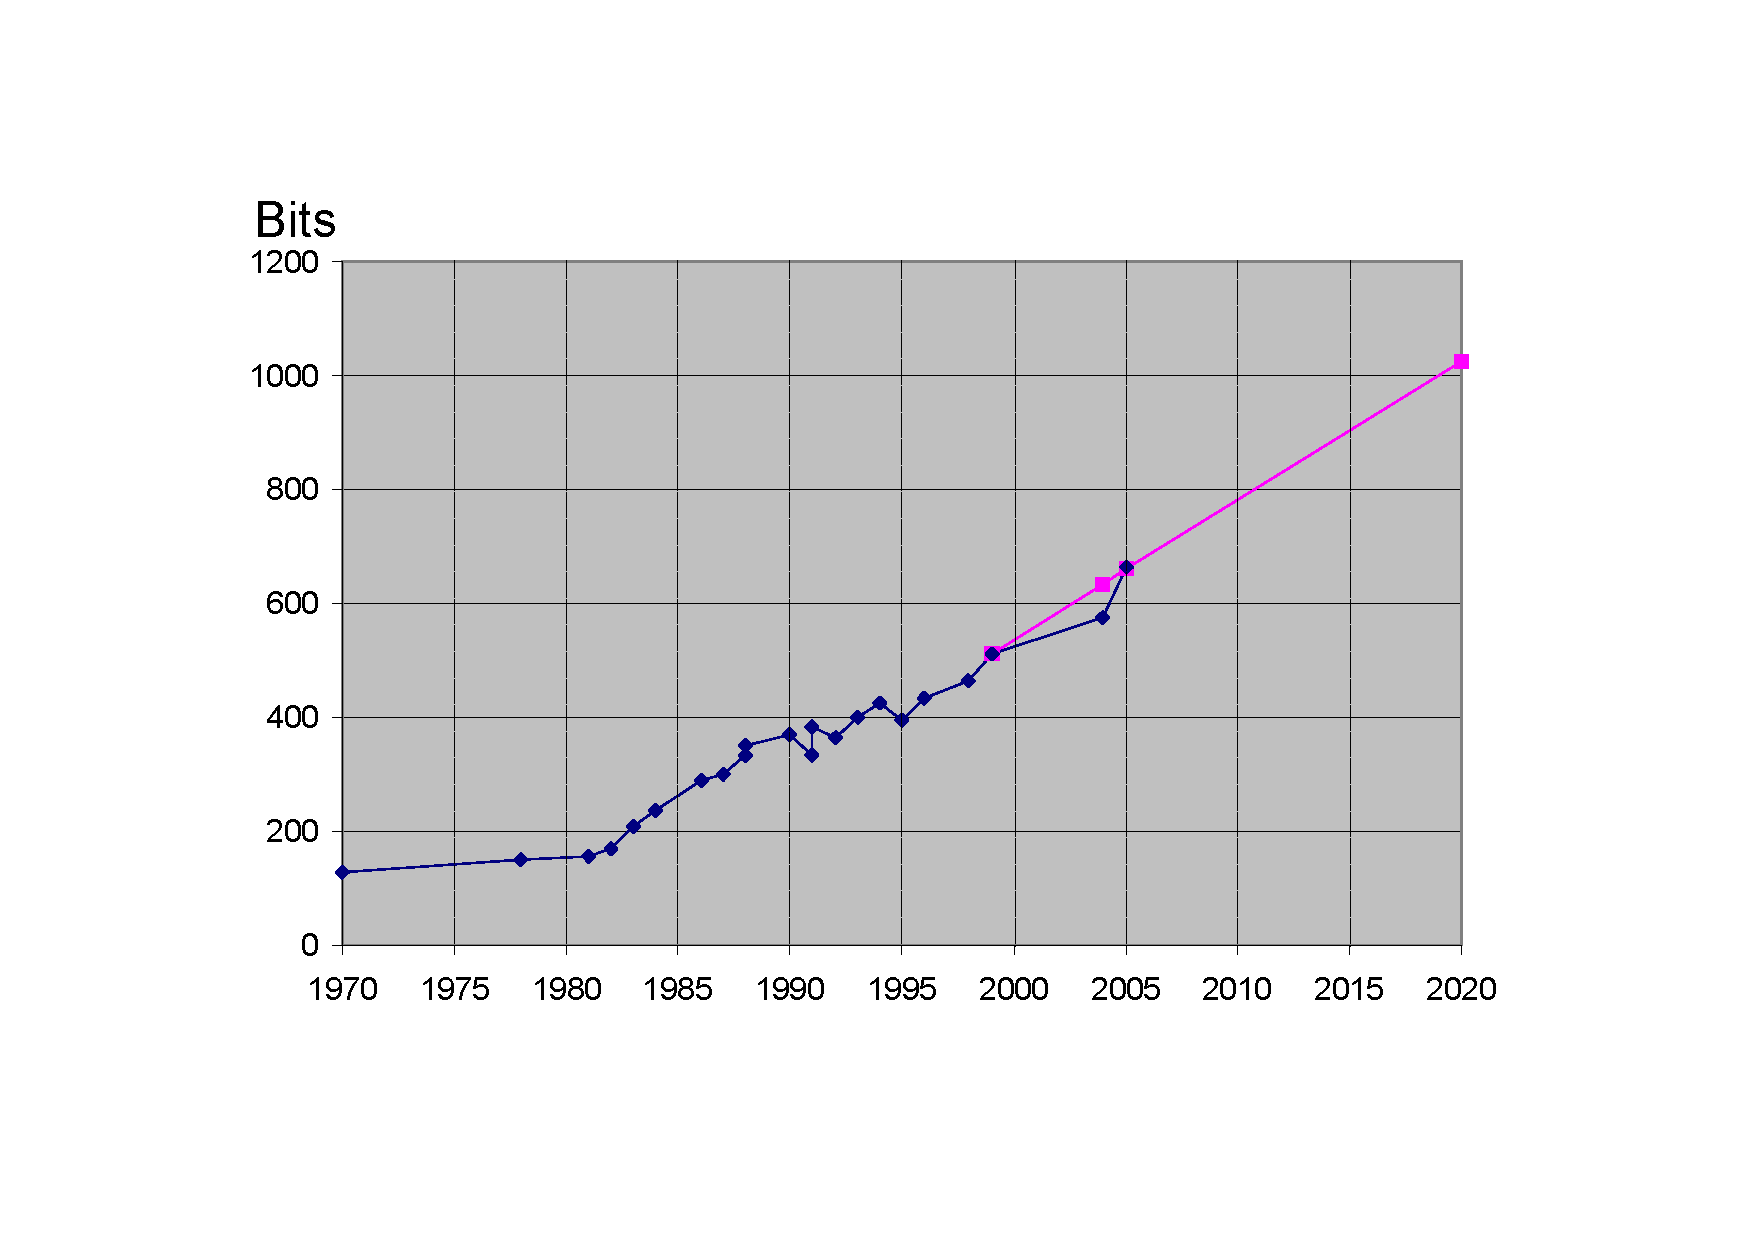
\includegraphics[scale=0.70, clip, viewport=50 20 700 430]{figures/PrognoseRSAFaktorisierungSecorvo.pdf}
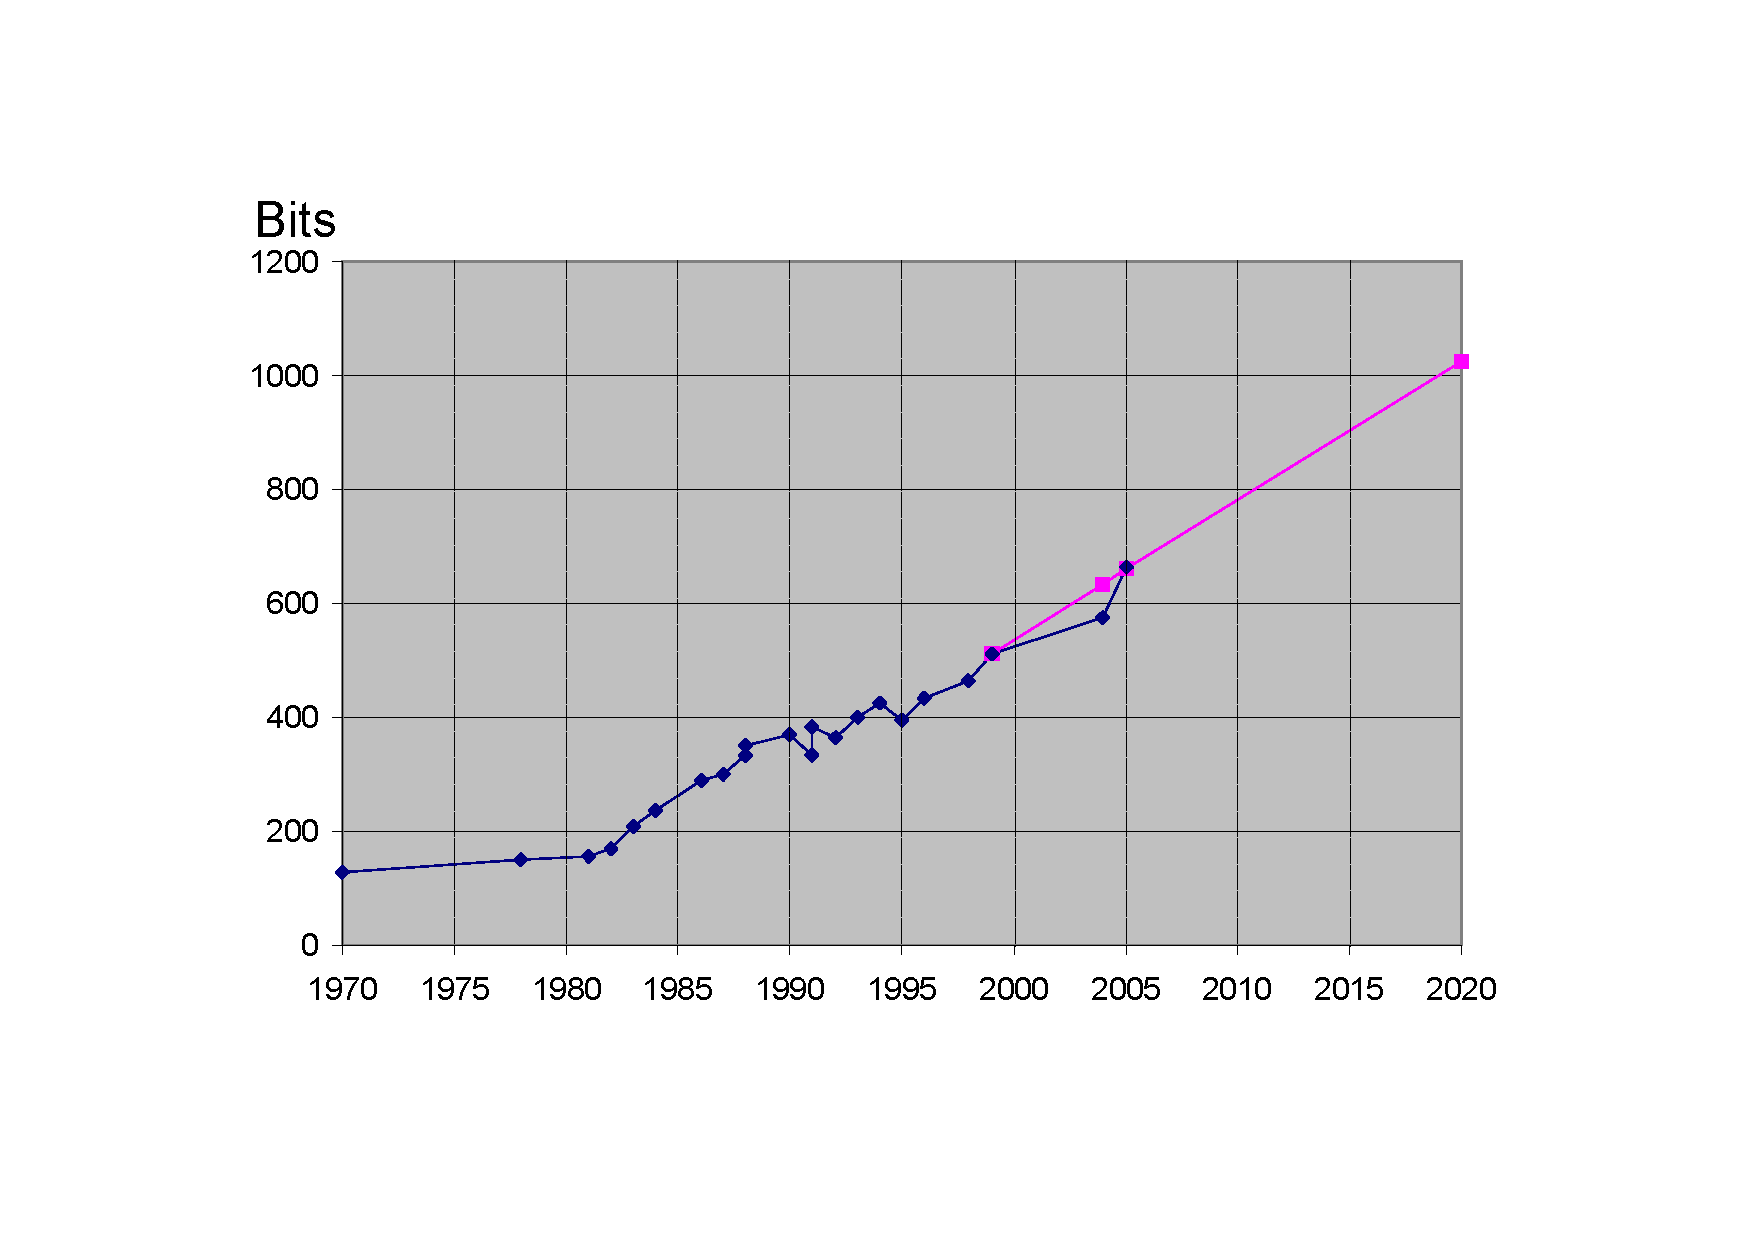
\includegraphics[scale=0.64, clip, viewport=-20 0 680 520]{figures/PrognoseRSAFaktorisierungSecorvo.pdf}
% Parameter von includegraphics: scale, x, y, dx, dy
% dx, dy spezifiziert die Ausdehnung, die man dem Bildes spendiert.
%      Ist dy zu klein, wird das Bild oben abgeschnitten
% x, y sagt, ab wo der Rahmen um das Bild gezeichnet wird.
%      Ist z.B. x=50, sind der linke Rahmenstrich und Teile des linken
%      Teiles des Bildes nicht zu sehen.
% scale dehnt Rahmenlinie und Bild aus -> Sitenrand wird bei 0.7 z.B. kleiner.
}
\caption{Vorhersage �ber die zuk�nftigen Faktorisierungsrekorde verglichen
mit aktuellen Resultaten (Quelle Secorvo)}
\label{secorvo-factorisation-forecast}
\end{center}
\end{figure}

H�lt die Prognose, dann ist die Faktorisierung eines RSA-Moduls der L�nge
1024 Bit in 15 Jahren zu erwarten.




\clearpage  % Erzwingt, dass alle Floating Objekte (z.B. Grafiken VORHER
            % geschrieben werden ! (sonst wurde Kapitel 4.11.4 begonnen,
            % und die Secorvo-Grafik auf er Folgeseite UNTER die Fussnote
            % geschoben. Au�erdem wahrscheinlich auch Zeilenumbruch,
            % egal, ob nach der Garfik noch Platz ist.
% ++++++++++++++++++++++++++++++++++++++++++++++++++++++++++++++++++++++++++
\vspace{6ex}
\begin{center}
\fbox{\parbox{15cm}{
    \emph{Hermann Hesse\footnotemark:}\\
    Damit das M�gliche entsteht, muss immer wieder das Unm�gliche 
    versucht werden.
}}
\end{center}
\addtocounter{footnote}{0}\footnotetext{%
    Hermann Hesse, deutsch-schweizerischer Schriftsteller und Nobelpreistr�ger, 
    02.07.1877$-$09.08.1962.}
% ++++++++++++++++++++++++++++++++++++++++++++++++++++++++++++++++++++++++++

\subsection{Status der Faktorisierung von konkreten gro�en Zahlen}
\label{NoteFactorisation}

Ausf�hrliche �bersichten �ber die Rekorde im Faktorisieren
zusammengesetzter Zahlen \index{Faktorisierung!Faktorisierungsrekorde}
mit unterschiedlichen Methoden finden sich auf den folgenden Webseiten:
\vspace{-10pt}
\begin{itemize}
\item[]
     \href{http://www.crypto-world.com}
  {\texttt{http://www.crypto-world.com}} \\
     \href{http://www.tutorgig.com/ed/RSA\_number}
  {\texttt{http://www.tutorgig.com/ed/RSA\_number}}  ~~ The RSA Factoring Challenge \\
%  {\texttt{http://www.tutorgig.com/ed/RSA\_number}}\footnote{%
%Diese Seite war Ende Mai 2005 nicht ganz auf dem aktuellen Stand: RSA-200 fehlte.}. \\
     \href{http://en.wikipedia.org/wiki/Integer_factorization_records}
  {\texttt{http://en.wikipedia.org/wiki/Integer\_factorization\_records}}
\end{itemize}

Der aktuelle Rekord (Stand Mai 2005) mit der GNFS-Methode (General Number
Field Sieve) \index{General Number Field Sieve (GNFS)} liegt in der Zerlegung
einer allgemeinen $200$-stelligen Dezimalzahl in ihre beiden Primfaktoren.

\vskip +10pt
Die letzten Rekorde\footnote{%
Die  "`RSA-Zahlen"' sind gro�e semiprime Zahlen (d.h. Zahlen, die genau aus
2 Primfaktoren bestehen)\index{Zahlen!semiprime}. Sie wurden von der Firma
RSA Security generiert und ver�ffentlicht, und sie bilden die "`RSA Factoring
Challenge"': In diesem Wettbewerb werden die Primfaktoren dieser Zahlen
gesucht.
Siehe \href{http://www.rsa.com/rsalabs/node.asp?id=2092}
   {\texttt{http://www.rsa.com/rsalabs/node.asp?id=2092}}.

In der ersten RSA-Factoring-Challenge wurden die Zahlen, von RSA-100 bis
RSA-500, gem�� der Anzahl ihrer Dezimalstellen benannt; die zweite
RSA-Factoring-Challenge benannte die Zahlen anhand der Anzahl ihrer
Bin�rstellen. Innerhalb des zweiten Wettbewerbs sind Geldpreise f�r die
erfolgreiche Faktorisierung von RSA576 bis RSA2048 ausgelobt (RSA576, RSA640
etc. in 64-er Schritten). 
Die Zahl RSA617 bildet eine Ausnahme, da sie vor der �nderung des 
Namensschemas erzeugt wurde.

Die Forscher um Prof. Jens Franke (von der Universit�t Bonn, dem BSI und dem
CWI) sind nicht auf die Geldpreise aus, sondern wollen die Grenzen der
Forschung ausdehnen. Dadurch werden Aussagen �ber notwendige Minimall�ngen
f�r sichere RSA-Moduli fundierter. 

Die "`C-Zahlen"' stammen aus dem Cunningham-Projekt:
\href{http://www.cerias.purdue.edu/homes/ssw/cun/}
     {\texttt{http://www.cerias.purdue.edu/homes/ssw/cun/}}
                                                               } 
mit Faktorisierungsverfahren f�r zusammengesetzte Zahlen
sind in der folgenden Tabelle~\ref{factorizationrecords} aufgef�hrt:

\begin{table}[ht]
\begin{center}
\begin{tabular}{|c|cccc|}
\hline
   & {\bf Dezimalstellen} & {\bf Bin�rstellen} & {\bf Faktorisiert am} & {\bf Faktorisiert von} \\
\hline
	C307 & 		307 & 1017 &  Mai, 2007 & Jens Franke et al. \\
	RSA-200 & 	200 & 663 & Mai, 2005 & Jens Franke et al. \\
	RSA640\footnotemark & 	193 & 600 & November, 2005 & Jens Franke et al. \\
	C176 & 		176 & 583 & Mai, 2005 & Kazumaro Aoki et al. \\
	RSA576 & 	174 & 576 & Dezember, 2003 & Jens Franke et al. \\
	RSA-160 & 	160 & 530 & April, 2003 & Jens Franke et al. \\
	C158 & 		158 & 523 & Januar, 2002 & Jens Franke et al. \\
	RSA-155	&	155 & 512 & August, 1999 & Herman te Riele et al. \\
\hline
\end{tabular}
\caption{Die derzeitigen Faktorisierungsrekorde (Stand Juli 2009)}    % Eyecatcher_neue-Mersenne
\label{factorizationrecords}
\end{center}
\end{table}
\footnotetext{%
Eine Arbeitsgruppe des BSI hat die mit 20.000 US-Dollar dotierte Challenge
RSA-640 mit Hilfe der GNFS-Methode gel�st. Die Forscher ben�tigten f�r die
Zerlegung der Zahl in ihre beiden 320 Bit langen Primfaktoren rund f�nf
Monate Rechenzeit.\\
Die RSA-Laboratorien schreiben ihre Challenges schon seit Anfang der
90er-Jahre aus. Die n�chst gr��ere Challenge ist nun die mit 30.000
US-Dollar dotierte RSA-704.\\
Siehe:
\href{http://www.heise.de/newsticker/meldung/print/65957}
{\texttt{http://www.heise.de/newsticker/meldung/print/65957}}
}
%be_2005: Erzwingen, dass die Abb. noch in diesem Kapitel !


Im Folgenden werden diese letzten Rekorde etwas ausf�hrlicher erl�utert.
Die beiden dabei benutzten Methoden GNFS und SNFS werden kurz z.B. auf
den ff. Webseiten dargestellt:
\index{General Number Field Sieve (GNFS)}
\index{Special Number Field Sieve (SNFS)}
\vspace{-10pt}
\begin{itemize}
\item[]
      \href{http://en.wikipedia.org/wiki/Special_number_field_sieve}
   {\texttt{http://en.wikipedia.org/wiki/Special\_number\_field\_sieve}} \\
      \href{http://en.wikipedia.org/wiki/General_number_field_sieve}
   {\texttt{http://en.wikipedia.org/wiki/General\_number\_field\_sieve}}
\end{itemize}
%\vspace{-10pt}


% --------------------------------------------------------------------------
\vskip +20pt
\paragraph{RSA-155} \label{RSA-155} \index{RSA-155} 
\mbox{} % f�r Zeilenumbruch, da er // allein nicht mag ! xxxxxxxxx

Am 22. August 1999 fanden niederl�ndische Forscher die L�sung dieser 
RSA-Challenge. Sie zerlegten eine $155$-stellige Zahl in ihre beiden $78$-stelligen
Primfaktoren (vergleiche Kapitel~\ref{chptSecurityParam}).
Mit der $512$ Bit-Zahl RSA-155 war eine {\em magische} Grenze erreicht.



% --------------------------------------------------------------------------
\vskip +20pt
\paragraph{C158} \label{C158} \index{C158} 
\mbox{} % f�r Zeilenumbruch, da er \\ allein nicht mag ! xxxxxxxxx
\hypertarget{C158-chap3}{}

Am 18. Januar 2002 zerlegten Forscher der Universit�t Bonn\footnote{%
\href{http://www.uni-bonn.de/Aktuelles/Pressemitteilungen/pm02/pm035-02.html}
{\texttt{http://www.uni-bonn.de/Aktuelles/Pressemitteilungen/pm02/pm035-02.html}}} 
mit der GNFS-Methode (General Number Field Sieve) \index{General Number
Field Sieve (GNFS)} eine $158$-stellige Dezimalzahl in ihre beiden Primfaktoren 
(diese haben 73 und 86 Dezimalstellen).

Dieser Rekord fand deutlich weniger Aufmerksamkeit in der Presse als die
L�sung von RSA-155.

Die Aufgabe der Bonner Wissenschaftler entsprang auch nicht einer Challenge,
sondern die Aufgabe war, die letzten Primfaktoren der Zahl $2^{953}+1$ 
zu finden (siehe~ ``Wanted List'' des Cunningham-Projekts\index{Cunningham-Projekt}%
\footnote{%
Cunningham-Projekt: \href{http://www.cerias.purdue.edu/homes/ssw/cun/}
                 {\texttt{http://www.cerias.purdue.edu/homes/ssw/cun/}}}). 

Die 6 kleineren, schon vorher gefundenen Primfaktoren dieser Zahl waren:
$$
\begin{array}{c}
        3, 1907, 425796183929, \\ 
        1624700279478894385598779655842584377, \\
        3802306738549441324432139091271828121 \quad{\rm und} \\ 
        128064886830166671444802576129115872060027.
\end{array}
$$
\begin{sloppypar}
Die drei kleinsten Faktoren k�nnen leicht\footnote{%
Z.B. mit CrypTool\index{CrypTool} �ber das Men� 
{\bf Einzelverfahren \textbackslash{} RSA-Kryptosystem \textbackslash{} 
Faktorisieren einer Zahl}. \\
In sinnvoller Zeit zerlegt CrypTool Zahlen bis 250 Bit L�nge.
Zahlen gr��er als 1024 Bit werden zur Zeit von CrypTool nicht angenommen.
}
bestimmt werden.
Die n�chsten drei Primfaktoren wurden von P.~Zimmerman%
\footnote{\href{http://www.loria.fr/zimmerma/ecmnet}{\tt http://www.loria.fr/\~{}zimmerma/ecmnet}}, 
T.~Grandlund%
\footnote{\href{http://www.swox.se/gmp/}{\tt http://www.swox.se/gmp/}}
und R. Harley in den Jahren 1999 und 2000 mit der Methode der Elliptischen
Kurven gefunden.
\end{sloppypar}

Als letzter Faktor blieb der sogenannte Teiler  "`C158"',
von dem man bis dahin wusste, dass er zusammengesetzt ist, aber man kannte
seine Primfaktoren nicht (die folgenden drei Zeilen sind eine einzige Zahl):
$$
\begin{array}{c}
39505874583265144526419767800614481996020776460304936 \\
45413937605157935562652945068360972784246821953509354 \\
4305870490251995655335710209799226484977949442955603
\end{array}
$$
Die Faktorisierung von C158 ergab die beiden 73- und 86-stelligen Primfaktoren:
$$
\begin{array}{c}
3388495837466721394368393204672181522815830368604993048084925840555281177
\end{array}
$$
und
$$
\begin{array}{c}
1165882340667125990314837655838327081813101 \\
2258146392600439520994131344334162924536139.
\end{array}
$$
Damit wurde die Zahl $2^{953}+1$ vollst�ndig in ihre 8 Primfaktoren zerlegt.

\noindent\begin{minipage}{\textwidth}
\vspace{3ex}
Verweise:
\vspace{-10pt}
\begin{itemize}
\item[]   \url{http://www.loria.fr/~zimmerma/records/gnfs158}\\
          \url{http://www.crypto-world.com/FactorRecords.html}\\
          \url{http://www.crypto-world.com/announcements/c158.txt}
\end{itemize}
\end{minipage}
\vspace{24pt}



% --------------------------------------------------------------------------
\vskip +20pt
\paragraph{RSA-160} \label{RSA-160} \index{RSA-160}\mbox{}
\hypertarget{RSA-160-chap3}{}

Am 1. April 2003 zerlegten Forscher der Universit�t Bonn\footnote{%
          \href{http://www.loria.fr/~zimmerma/records/rsa160}
       {\texttt{http://www.loria.fr/\~{}zimmerma/records/rsa160}} \\
          \href{http://www.loria.fr/~zimmerma/records/factor.html}
       {\texttt{http://www.loria.fr/\~{}zimmerma/records/factor.html}} \\
          \href{http://www.crypto-world.com/FactorWorld.html}
       {\texttt{http://www.crypto-world.com/FactorWorld.html}}
} 
mit der GNFS-Methode (General Number Field Sieve) \index{General Number
Field Sieve (GNFS)} eine $160$-stellige Zahl in ihre beiden Primfaktoren 
(diese haben jeweils 80 Dezimalstellen).

Die Berechnungen dazu fanden auch im Bundesamt f�r Sicherheit in der 
Informationstechnik (BSI) in Bonn statt\footnote{%
Das BSI \index{BSI} erstellt jedes Jahr ein Papier �ber die Eignung von
Kryptoalgorithmen, mit denen Signaturen erzeugt werden k�nnen,         
die den Vorgaben des deutschen Signaturgesetzes gen�gen.
Bei dieser Erstellung werden Experten aus Wirtschaft und Wissenschaft
beteiligt. Um die Eignung von Signaturverfahren zu beurteilen, deren
Schwierigkeit auf dem Faktorisierungsproblem beruht,
kooperiert das BSI auch mit Forschern der Universit�t Bonn.
Weitere Informationen zu Kryptoalgorithmen finden Sie auf den BSI-Internetseiten unter:
   \href{http://www.bsi.bund.de/esig/basics/techbas/krypto/index.htm}
{\texttt{http://www.bsi.bund.de/esig/basics/techbas/krypto/index.htm}}
}.

Die 160-stellige Dezimalzahl stammt von der alten Challenge-Liste von RSADSI.
Diese wurde nach der Faktorisierung von RSA-155 (RSA512) zur�ckgezogen.
Die Primfaktoren von RSA-160 waren aber nicht bekannt.
Deshalb ist dieser Rekord von Prof.\ Frankes Team immer noch die L�sung 
einer alten Challenge, f�r die es aber von RSADSI kein Geld gibt.

Die zusammengesetzte Zahl "`RSA-160"' lautet (die folgenden drei Zeilen 
sind eine einzige Zahl):
$$
\begin{array}{c}
215274110271888970189601520131282542925777358884567598017049 \\
767677813314521885913567301105977349105960249790711158521430 \\
2079314665202840140619946994927570407753
\end{array}
$$
Die Faktorisierung von RSA-160 ergab die beiden Primfaktoren:
$$
\begin{array}{c}
p = 45427892858481394071686190649738831 \\         
    656137145778469793250959984709250004157335359
\end{array}
$$
und
$$
\begin{array}{c}
q = 47388090603832016196633832303788951 \\
    973268922921040957944741354648812028493909367
\end{array}
$$

Die Berechnungen erfolgten zwischen Dezember 2002 und April 2003.
\vspace{24pt}



% ammmmmmmmmmma
% 
% RSA-576 faktorisiert 
% Am 27.04.2004 ging die Nachricht durch
% die Ticker, dass die 576-bit-Challenge der
% Firma RSA gel�st sei. Tats�chlich wurde
% die 174 Dezimalstellen lange Zahl bereits
% am 03.12.2003 zerlegt. Die Faktorisierung
% gelang einem Team der Universit�t Bonn
% um Professor Franke mit Unterst�tzung
% durch das Institut f�r Experimentelle Mathematik
% in Essen und das BSI. Die verteilte
% Berechung erfolge auf einem Linux-
% Cluster mit 144 PCs (400 MHz, Pentium II)
% und verwendete den General Number Field
% Sieve-Algorithmus ? mit einem Aufwand
% von umgerechnet 13.200 MIPS-Jahren.
% Interessant dabei: Dieser Faktorisierungserfolg
% best�tigt die Prognose, die Secorvo
% vor drei Jahren auf der Basis der Faktorisierungserfolge
% der vergangenen 30 Jahre
% gestellt hat (siehe Bild), und die weit weniger
% dramatisch ausfiel als viele Expertenwarnungen
% und die Erwartung des BSI.
% Danach w�re 2004 erstmals die Faktorisierung
% einer 630 bit langen Zahl zu erwarten
% gewesen ? was nun eher unwahrscheinlich
% erscheint. Selbst die fr�hestens f�r das
% Jahr 2020 vorausgesagte Faktorisierung
% eines 1024 bit langen RSA-Schl�ssels
% k�nnte sich daher noch als zu pessimistische
% Bef�rchtung erweisen ? allen Warnern
% zum Trotz, die seit Jahren Schl�ssell
% �ngen von 2048 bit und mehr empfehlen
% oder gar das baldige Ende von RSA prophezeihen.
% 
% ammmmmmmmmmmz




% --------------------------------------------------------------------------
\vskip +20pt
\hypertarget{RSA-200-chap3}{}
\paragraph{RSA-200} \label{RSA-200} \index{RSA-200}\mbox{}
\nopagebreak

Am 9. Mai 2005 meldete die Forschergruppe von Prof. Jens Franke der Universit�t Bonn\footnote{%
   \href{http://www.loria.fr/~zimmerma/records/rsa200}
{\texttt{http://www.loria.fr/\~{}zimmerma/records/rsa200}}}, dass sie
gemeinsam mit Kollegen des Amsterdam Centrum voor Wiskunde en Informatica
einen neuen Weltrekord im Faktorisieren aufstellten. 

Sie zerlegten mit der GNFS-Methode (General Number Field Sieve) \index{General Number
Field Sieve (GNFS)} eine $200$-stellige Zahl in ihre beiden Primfaktoren 
(diese haben jeweils 100 Dezimalstellen).

Die zusammengesetzte Zahl "`RSA-200"' lautet (die folgenden drei Zeilen 
sind eine einzige Zahl):
$$
\begin{array}{c}
2799783391122132787082946763872260162107044678695542853756000992932 \\
6128400107609345671052955360856061822351910951365788637105954482006 \\
576775098580557613579098734950144178863178946295187237869221823983
\end{array}
$$
Die Faktorisierung von RSA-200 ergab die beiden Primfaktoren:
$$
\begin{array}{c}
p = 35324619344027701212726049781984643686711974001976 \\
    25023649303468776121253679423200058547956528088349
\end{array}
$$
und
$$
\begin{array}{c}
q = 79258699544783330333470858414800596877379758573642 \\
    19960734330341455767872818152135381409304740185467
\end{array}
$$

Die Berechnungen erfolgten zwischen Dezember 2003 und Mai 2005.
Die Faktorisierung durch die Gruppe um Bahr, B�hm, Franke, Kleinjung, 
Montgomery und te Riele hatte also knapp 17 Monate gedauert.
Der Rechenaufwand lag bei umgerechnet etwa 120.000 MIPS-Jahren\footnote{%
Ein MIPS-Jahr (MY) ist die Anzahl von Operationen, die eine Maschine, 
welche eine Million Integeroperationen pro Sekunde (MIPS)
ausf�hrt, in einem Jahr bew�ltigt. Zur Illustration: ein INTEL 
Pentium 100 Prozessor hat etwa 50 MIPS.
F�r die Zerlegung eines 2048-Bit-Moduls br�uchte man ca. {$8,5 \cdot 
10^{40}$ MY}.}.
\vspace{24pt}





% --------------------------------------------------------------------------
\vskip +20pt
\paragraph{C307 / M1039} \label{C307} \index{C307} \index{M1039} 
\mbox{} % f�r Zeilenumbruch, da er \\ allein nicht mag ! xxxxxxxxx
\hypertarget{C307-chap3}{}

Im Mai 2007 meldeten Prof. Franke, Prof. Kleinjung (von der Universit�t Bonn),
das japanische Telekommunikationsunternehmen NTT und Prof. Arjen Lenstra von
der Polytechnischen Hochschule in Lausanne, dass sie mit der SNFS-Methode
(Special Number Field Sieve) \index{Special Number Field Sieve (SNFS)}
innerhalb von 11 Monaten
eine $307$-stellige Dezimalzahl in ihre beiden Primfaktoren zerlegten
(diese haben 80 und 227 Dezimalstellen).

Die Aufgabe der Wissenschaftler entsprang nicht einer Challenge, sondern
die Aufgabe war, die letzten Primfaktoren der Mersenne-Zahl $2^{1039}+1$ 
zu finden (siehe~ \glqq Wanted List\grqq~ des Cunningham-Projekts\index{Cunningham-Projekt}%
\footnote{%
Cunningham-Projekt: \href{http://www.cerias.purdue.edu/homes/ssw/cun/}
                 {\texttt{http://www.cerias.purdue.edu/homes/ssw/cun/}}\\
Cunningham-Tabelle: \href{http://homes.cerias.purdue.edu/~ssw/cun/pmain1206}
                 {\texttt{http://homes.cerias.purdue.edu/\~{}ssw/cun/pmain1206}}\\
Die Zahlen in der Cunningham-Tabelle werden folgenderma�en geschrieben:\\
\glqq (2,n)-\grqq~ bedeutet $2^{n}-1$;~~~
\glqq (2,n)+\grqq~ bedeutet $2^{n}+1$.\\
Um die Gr��enordnung einer Zerlegung anzudeuten schreibt man $p<n>$ oder $c<n>$,
wobei \glqq n\grqq~ die Anzahl der Dezimalstellen ist und \glqq p\grqq~ und \glqq c\grqq~
bedeuten, dass die Zahl eine Primzahl oder eine zusammengesetzte Zahl ist.\\
$2^{1039}-1 = p7 * c307 = p7 * p80 * p227$ \\
Genauer erkl�rt wird dies auf der CUN-Seite folgenderma�en:\\
\glqq 2,651+ means $2^{651} + 1$ and the size (c209 means 209 decimal digits)
of the
number which was factored.  Then come the new factor(s), the discoverer and
the method used.  Recently, only the multiple polynomial quadratic sieve
(ppmpqs), the elliptic curve method (ecm) and the number field sieve (nfs)
have been used.  `hmpqs' stands for hypercube multiple polynomial quadratic
sieve.  Under `new factors', `p90' means a 90-digit prime and `c201' is a
201-digit composite number.\grqq. 
}).\\


Die Zahl $2^{1039}-1$ besteht aus 3 Primfaktoren: Der kleinste Faktor
$p7 = 5080711$ war schon l�nger bekannt.\footnote{%
Er kann mit CrypTool\index{CrypTool} �ber das Men� 
{\bf Einzelverfahren \textbackslash{} RSA-Kryptosystem \textbackslash{} 
Faktorisieren einer Zahl} gefunden werden --- mit den Algorithmen von Brent,
Williams oder Lenstra, mit denen man gut \glqq relativ\grqq~ kleine Faktoren
abspalten kann. \\
In sinnvoller Zeit zerlegt CrypTool vollst�ndig Zahlen bis 250 Bit L�nge.
}

Zur vollst�ndigen Faktorisierung musste der zweite Faktor (Koteiler) "`C307"'
zerlegt werden: Bis dahin wusste man nur, dass er zusammengesetzt ist, aber man
kannte weder die Anzahl seiner Primfaktoren, noch die Primfaktoren selbst.
Die folgenden f�nf Zeilen sind eine einzige Zahl:
$$
\begin{array}{c}
C307 =1159420574072573064369807148876894640753899791702017724986868353538\\
8224838599667566080006095408005179472053993261230204874402860435302\\
8619141014409345351233471273967988850226307575280937916602855510550\\
0425810771176177610094137970787973806187008437777186828680889844712\\
822002935201806074755451541370711023817
\end{array}
$$
Die Faktorisierung von C307 ergab die beiden 80- und 227-stelligen Primfaktoren:
$$
\begin{array}{c}
p80 = 558536666199362912607492046583159449686465270184\\
      88637648010052346319853288374753
\end{array}
$$
und
$$
\begin{array}{c}
p227 = 207581819464423827645704813703594695162939708007395209881208\\
       387037927290903246793823431438841448348825340533447691122230\\
       281583276965253760914101891052419938993341097116243589620659\\
       72167481161749004803659735573409253205425523689
.
\end{array}
$$
Damit wurde die Zahl $2^{1039}-1$ vollst�ndig in ihre 3 Primfaktoren zerlegt.

\noindent\begin{minipage}{\textwidth}
\vspace{3ex}
Verweise:
\vspace{-10pt}
\begin{itemize}
\item[]   \url{http://www.loria.fr/~zimmerma/records/21039-}\\
          \url{http://www.crypto-world.com/announcements/m1039.txt}\\
          \url{http://www.crypto-world.com/FactorAnnouncements.html}\\
          \url{http://www1.uni-bonn.de/pressDB/jsp/pressemitteilungsdetails.jsp?detailjahr=2007&detail=160}
\end{itemize}
\end{minipage}






% --------------------------------------------------------------------------
\vskip +50pt
\paragraph{Gr��enordnung faktorisierter Zahlen im Vergleich zu auf Primalit�t getesteter Zahlen}
\mbox{}

Wie man sieht, sind die gr��ten (aus 2 Primfaktoren) zusammengesetzten
Zahlen, die man faktorisieren kann, deutlich kleiner als die Zahlen mit
einer speziellen Struktur, f�r die Primzahltests\index{Primzahltest} in
der Lage sind, Aussagen �ber ihre Primalit�t zu treffen (siehe Kapitel 
\ref{search_for_very_big_primes},~\ref{primality_tests} und
\ref{spezialzahlentypen}).


% be_2005_UPDATEN_if-new-mersenne-prime-appears   % Eyecatcher_neue-Mersenne
L�nge in Bit der derzeitigen Weltrekorde:\\
$$  ~~~~~~~~~[RSA{-}200{-}Zahl] ~~\longleftrightarrow{}~~[43.~bekannte~Mersenne~Primzahl] $$
$$ 663 ~~ \longleftrightarrow{} ~~ 30.402.457 ~~~~~$$


%be_2005 - erzwungenes Blank und $$ um Pfeilzeichen, sonst setzt er Blanks an 
%          die falschen Stellen.
%        - Wenn man hier \~ statt nur ~ (au�erhalb der $$) schreibt, kommen
%          nachher Fussnoten mit 
%          {\bf Einzelverfahren \textbackslash{} Protokolle}
%          nur noch mit kaputten Schriftzeichen raus !



% --------------------------------------------------------------------------
\vskip +60pt
\subsection{Weitere aktuelle Forschungsergebnisse zu Primzahlen und Faktorisierung}
\label{FactorisationResearch}
Primzahlen sind Teil vieler hochaktueller Forschungsgebiete der Zahlentheorie. 
Die Fortschritte bei der Faktorisierung sind gr�� als noch vor 5 Jahren
gesch�tzt -- sie gehen nicht nur auf das Konto schnellerer Rechner, 
sondern sie sind auch in neuen Erkenntnissen begr�ndet.

Die Sicherheit des RSA-Algorithmus basiert auf der empirischen Beobachtung, dass die Faktorisierung gro�er ganzer 
Zahlen ein schwieriges Problem ist. Besteht wie beim RSA-Algorithmus der zugrunde liegende Modul $n$ aus dem Produkt 
zweier gro�er Primzahlen $p, q$ (typische L�ngen: $p, q$  $500-600$ bit, $n$ $1024$ bit), so l�sst sich 
$n=pq$ aus $p$ und $q$ leicht bestimmen, jedoch ist es mit den bisher bekannten Faktorisierungsalgorithmen nicht
m�glich, $p, q$ aus $n$ zu gewinnen. Nur mit Kenntnis von $p$ und $q$ l�sst sich jedoch der private aus dem 
�ffentlichen Schl�ssel ermitteln.

Die Entdeckung eines Algorithmus zur effizienten Faktorisierung von Produkten $n=pq$ gro�er Primzahlen w�rde daher 
den RSA-Algorithmus wesentlich beeintr�chtigen. Je nach Effizienz der Faktorisierung im Vergleich zur Erzeugung von 
$p, q, n$ m�sste der verwendete Modul $n$ (z.Zt. 1024 bit) erheblich vergr��ert oder --- im Extremfall --- auf den 
Einsatz des RSA ganz verzichtet werden.


% --------------------------------------------------------------------------
\vskip +20pt
\paragraph{Das Papier von Bernstein und seine Auswirkungen auf die Sicherheit
des RSA-Algorithmus} \label{RSABernstein} \index{Faktorisierung!Faktorisierungsproblem}
\mbox{} % f�r Zeilenumbruch, da er \\ allein nicht mag ! 
        % Braucht die Leerzeile danach auch noch !! bebebe ?

Die im November 2001 ver�ffentlichte Arbeit ``Circuits for integer
factorization: a proposal'' (siehe
\href{http://cr.yp.to/djb.html}{\texttt{http://cr.yp.to/djb.html}}) von
D.J. Bernstein \cite{nt:Bernstein2001} behandelt das Problem der 
Faktorisierung gro�er Zahlen.
Die Kernaussage des Papers besteht darin, dass es m�glich ist, die
Implementierung des General Number Field Sieve-Algorithmus (GNFS)
\index{General Number Field Sieve (GNFS)} so zu
verbessern, dass mit gleichem Aufwand wie bisher Zahlen mit 3-mal
gr��erer Stellenzahl (Bit-L�nge) faktorisiert werden k�nnen.

Wesentlich bei der Interpretation des Resultats ist die Definition des
Aufwandes: Als Aufwand wird das Produkt von ben�tigter Rechenzeit und
Kosten der Maschine (insbesondere des verwendeten Speicherplatzes)
angesetzt. Zentral f�r das Ergebnis des Papiers ist die Beobachtung, dass
ein wesentlicher Teil der Faktorisierung auf Sortierung zur�ckgef�hrt
werden kann und mit dem Schimmlerschen Sortierschema ein Algorithmus zur
Verf�gung steht, der sich besonders gut f�r den Einsatz von
Parallelrechnern eignet. Am Ende des Abschnittes 3 gibt Bernstein konkret
an, dass die Verwendung von $m^2$ Parallelrechnern mit jeweils gleicher
Menge an Speicherplatz mit Kosten in der Gr��enordnung von $m^2$
einhergeht --- genau so wie ein einzelner Rechner mit $m^2$ Speicherzellen.
Der Parallelrechner bew�ltigt die Sortierung von $m^2$ Zahlen jedoch
(unter Verwendung der o.~g.\ Sortierverfahrens) in Zeit proportional zu m,
wohingegen der Einprozessorrechner Zeit proportional $m^2$ ben�tigt.
Verringert man daher den verwendeten Speicherplatz und erh�ht --- bei
insgesamt gleich bleibenden Kosten --- die Anzahl der Prozessoren
entsprechend, verringert sich die ben�tigte Zeit um die Gr��enordnung
$1/m$. In Abschnitt 5 wird ferner angef�hrt, dass der massive Einsatz der
parallelisierten Elliptic Curve-Methode von Lenstra die Kosten der
Faktorisierung ebenfalls um eine Gr��enordnung verringert (ein
Suchalgorithmus hat dann quadratische statt kubische Kosten).  Alle
Ergebnisse von Bernstein gelten nur asymptotisch f�r gro�e Zahlen $n$.
Leider liegen keine Absch�tzungen �ber den Fehlerterm, d.h.  die
Abweichung der tats�chlichen Zeit von dem asymptotischen Wert, vor --- ein
Mangel, den auch Bernstein in seinem Papier erw�hnt. Daher kann zur Zeit
keine Aussage getroffen werden, ob die Kosten (im Sinne der Bernsteinschen
Definition) bei der Faktorisierung z.~Zt.\ verwendeter RSA-Zahlen
(1024$-$2048 bit) bereits signifikant sinken w�rden.

Zusammenfassend l�sst sich sagen, dass der Ansatz von Bernstein durchaus 
innovativ ist. Da die Verbesserung der 
Rechenzeit unter gleichbleibenden Kosten durch einen massiven Einsatz von 
Parallelrechnern erkauft wird, stellt sich die 
Frage nach der praktischen Relevanz. Auch wenn formal der Einsatz von einem 
Rechner �ber 1 sec  und  1.000.000 Rechnern 
f�r je 1/1.000.000 sec dieselben Kosten erzeugen mag, ist die 
Parallelschaltung von 1.000.000 Rechnern praktisch nicht 
(oder nur unter immensen Fixkosten, insbesondere f�r die Vernetzung der
Prozessoren) zu realisieren. Solche Fixkosten 
werden aber nicht in Ansatz gebracht.
Die Verwendung verteilter Ans�tze (distributed computing) �ber ein 
gro�es Netzwerk k�nnte einen Ausweg bieten. Auch hier m�ssten  
Zeiten und Kosten f�r Daten�bertragung einkalkuliert werden.

Solange noch keine (kosteng�nstige) Hardware oder verteilte Ans�tze 
entwickelt wurden, die auf 
dem Bernsteinschen Prinzip basieren, besteht noch keine akute Gef�hrdung
des RSA. Es bleibt zu kl�ren, ab welchen 
Gr��enordnungen von n die Asymptotik greift. 

Arjen Lenstra, Adi Shamir et.~al.\ haben das Bernstein-Paper analysiert 
\cite{nt:Lenstra2002}.
Als Ergebnis kommen Sie zu einer Bitl�ngen-Verbesserung der 
Faktorisierung um den Faktor 1.17 
(anstatt Faktor 3 wie von Bernstein erwartet).

Die Zusammenfassung ihres Papers ``Analysis of Bernstein's Factorization 
Circuit'' lautet:

``... Bernstein proposed a circuit-based implementation of
the matrix step of the number field sieve factorization algorithm. We
show that under the non-standard cost function used in [1], these circuits
indeed offer an asymptotic improvement over other methods but
to a lesser degree than previously claimed: for a given cost, the new
method can factor integers that are 1.17 times larger (rather than 3.01).
We also propose an improved circuit design based on a new mesh routing
algorithm, and show that for factorization of 1024-bit integers the
matrix step can, under an optimistic assumption about the matrix size,
be completed within a day by a device that costs a few thousand dollars.
We conclude that from a practical standpoint, the security of RSA relies
exclusively on the hardness of the relation collection step of the number
field sieve.''

Auch \href{http://www.rsasecurity.com/}{RSA Security} kommt in ihrer Analyse der Bernstein-Arbeit \cite{nt:RSA Security 2002} vom 8. April 2002 erwartungsgem��
zu dem Ergebnis, dass RSA weiterhin als ungebrochen betrachtet werden kann.

Die Diskussion ist weiterhin im Gang.

Zum Zeitpunkt der Erstellung dieses Absatzes (Juni 2002) war nichts
dar�ber bekannt, inwieweit die im Bernstein-Papier vorgeschlagenen
theoretischen Ans�tze realisiert wurden oder wieweit die Finanzierung
seines Forschungsprojektes ist.

\noindent\begin{minipage}{\textwidth}
\vspace{3ex}
Verweise:
\vspace{-10pt}
\begin{itemize}
  \item[] \href{http://cr.yp.to/djb.html}
               {\texttt{http://cr.yp.to/djb.html}} \\
          \href{http://www.counterpane.com/crypto-gram-0203.html\#6}
               {\texttt{http://www.counterpane.com/crypto-gram-0203.html\#6}} \\
          \href{http://www.math.uic.edu}
               {\texttt{http://www.math.uic.edu}} 
\end{itemize}
\end{minipage}



% --------------------------------------------------------------------------
\vskip +20pt
\paragraph{Das TWIRL-Device} \label{TWIRLDevice} \index{TWIRL-Device}
\mbox{} % f�r Zeilenumbruch, da er // allein nicht mag ! xxxxxxxxx

Im Januar 2003 ver�ffentlichten Adi Shamir und Eran Tromer vom Weizmann
Institute of Science den vorl�ufigen Draft {\em ``Factoring Large Numbers
with the TWIRL Device''}, in dem deutliche Bedenken gegen RSA-Schl�ssell�ngen
unter 1024 begr�ndet werden \cite{nt:Shamir2003}.

Das Abstract fasst ihre Ergebnisse folgenderma�en zusammen: ``The security of the RSA cryptosystem depends on the difficulty of factoring large integers. The best current factoring algorithm is the Number Field Sieve (NFS), and its most difficult part is the sieving step. In 1999 a large distributed computation involving thousands of workstations working for many months managed to factor a 512-bit RSA key, but 1024-bit keys were believed to be safe for the next 15-20 years. In this paper we describe a new hardware implementation of the NFS sieving step ... which is 3-4 orders of magnitude more cost effective than the best previously published designs ... . Based on a detailed analysis of all the critical components (but without an actual implementation), we believe that the NFS sieving step for 1024-bit RSA keys can be completed in less than a year by a \$10M device, and that the NFS sieving step for 512-bit RSA keys can be completed in less than ten minutes by a \$10K device. Coupled with recent results about the difficulty of the NFS matrix step ... this raises some concerns about the security of these key sizes.''

Eine ausf�hrliche Fassung findet sich auch in dem Artikel der beiden Autoren
in den RSA Laboratories CryptoBytes \cite{nt:Shamir2003a}.

Eine sehr gute Erl�uterung, wie der Angriff mit dem Generalized Number Field
Sieve (GNFS) \index{General Number Field Sieve (GNFS)} funktioniert und
welche Fortschritte sich ergaben, findet sich
in dem 3-seitigen Artikel in der DuD-Ausgabe Juni/2003 \cite{nt:Weis2003}.
Beim GNFS k�nnen 2 grundlegende Schritte unterschieden werden: 
der Siebungsschritt (Relationen sammeln) und die Matrix-Reduktion.
Auch wenn der Siebungsschritt hochgradig parallelisierbar ist, so dominiert
er doch den Gesamtrechenaufwand. Bisher haben Shamir und Tromer noch kein 
TWIRL-Device gebaut, jedoch ist der daf�r gesch�tzte Aufwand von 10 bis
50 Millionen Euro, um eine 1024-Bit Zahl in einem Jahr zu faktorisieren
f�r Geheimdienste oder gro�e kriminelle Organisationen keineswegs prohibitiv,
denn die \glqq Kosten f�r einen einzigen Spionagesatelliten sch�tzt man
z.B. auf mehrere Milliarden USD\grqq. Die Autoren empfehlen deshalb konkret,
m�glichst rasch sensible, bisher benutzte RSA-, Diffie-Hellman- oder 
ElGamal-Schl�ssel von bis zu 1024 Bit zu wechseln und Schl�ssel von 
mindestens 2048 Bit L�nge einzusetzen.
Auch f�r die geplante TCPA/Palladium-Hardware \index{Palladium} werden
2048-Bit RSA-Schl�ssel verwendet!

Damit erscheinen die aktuellen Empfehlungen des BSI, auf l�ngere 
RSA-Schl�ssell�ngen umzustellen, mehr als gerechtfertigt.



% --------------------------------------------------------------------------
\vskip +20pt
%\paragraph{``Primes in P'': Testen auf Primalit�t ist polynominal}
\paragraph{\glqq Primes in P\grqq: Testen auf Primalit�t ist polynominal}
\label{PrimesinP} \index{Primzahltest} 
\mbox{} % f�r Zeilenumbruch, da er // allein nicht mag ! xxxxxxxxx

Im August 2002 ver�ffentlichten die drei indischen Forscher M. Agrawal, 
N. Kayal und N. Saxena ihr Paper {\em \glqq PRIMES in P\grqq}  %{\em ``PRIMES in P''} 
�ber einen neuen Primzahltest-Algorithmus, genannt AKS\index{AKS} \cite{nt:Agrawal2002}.
Sie entdeckten einen polynominalen\index{Polynom} deterministischen Algorithmus, um zu entscheiden, ob eine gegebene Zahl prim ist oder nicht.

Die Bedeutung dieser Entdeckung liegt darin, dass sie Zahlentheoretiker mit neuen Einsichten und M�glichkeiten f�r die weitere Forschung versorgt. Viele Menschen haben im Lauf der Jahrhunderte nach einem polynominalen Primzahltest gesucht, so dass dieses Ergebnis einen theoretischen Durchbruch darstellt. Es zeigt sich immer wieder, dass aus schon lange bekannten Fakten neue Ergebnisse generiert werden k�nnen.

Aber selbst die Autoren merken an, dass andere bekannte Algorithmen (z.B. ECPP) schneller sein k�nnen. Der neue Algorithmus funktioniert f�r alle positiven ganzen Zahlen. Dagegen verwendet das GIMPS-Projekt den Lucas-Lehmer-Primzahltest, der besondere Eigenschaften der Mersennezahlen ausnutzt. Dadurch ist der Lucas-Lehmer-Test viel schneller und erlaubt, Zahlen mit Millionen von Stellen zu testen, w�hrend generische Algorithmen auf Zahlen mit einigen tausend Stellen beschr�nkt sind. Nachteil der bisherigen schnellen Verfahren ist, dass sie probabilistisch sind, also ihr Ergebnis h�chstwahrscheinlich, aber nicht ganz sicher ist.

\enlargethispage{20pt}
\noindent Aktuelle Forschungsergebnisse dazu finden sich z.B. auf: 
\vspace{-10pt}
\begin{itemize}
  \item[] \href{http://www.mersenne.org/}
               {\texttt{http://www.mersenne.org/}} \\
          \href{http://fatphil.org/maths/AKS/}
               {\texttt{http://fatphil.org/maths/AKS/}} Originaltext in Englisch\\
          \href{http://ls2-www.cs.uni-dortmund.de/lehre/winter200203/kt/material/primes.ps}
               {\texttt{http://ls2-www.cs.uni-dortmund.de/lehre/winter200203/kt/material/primes.ps}}\\\hspace*{2em}Gute Erl�uterung in Deutsch von Thomas Hofmeister.
\end{itemize}

\vskip +10 pt




% ++++++++++++++++++++++++++++++++++++++++++++++++++++++++++++++++++++++++++
\newpage
\begin{center}
\fbox{\parbox{15cm}{{\em Joanne K.\index{Rowling, Joanne} Rowling\footnotemark:}\newline
Viel mehr als unsere F�higkeiten sind es 
unsere Entscheidungen ..., die zeigen, wer wir wirklich sind.}}
\end{center}

\addtocounter{footnote}{0}\footnotetext{Joanne K. Rowling, \glqq Harry Potter
und die Kammer des Schreckens'', Carlsen, (c) 1998,
letztes Kapitel \glqq Dobbys Belohnung'', S. 343, Dumbledore.}
% ++++++++++++++++++++++++++++++++++++++++++++++++++++++++++++++++++++++++++
\section{Anwendungen asymmetrischer Kryptographie mit Zahlenbeispielen}

In der modernen Kryptographie \index{Kryptographie!moderne} werden die Ergebnisse
der modularen Arithmetik extensiv angewandt. Hier werden exemplarisch einige
wenige Beispiele aus der Kryptographie mit kleinen\footnote{%
\glqq Klein'' bedeutet beim RSA-Verfahren, dass die Bitl�ngen der Zahlen sehr
viel kleiner sind als $1024$ Bit (das sind $308$ Dezimalstellen). 
$1024$ Bit gilt im Moment in der Praxis als Mindestl�nge f�r einen sicheren Certification
Authority-RSA-Modul.
} Zahlen vorgestellt.

Die Chiffrierung eines Textes besteht darin, dass man aus einer Zeichenkette
(Zahl) durch Anwenden einer Funktion (mathematische Operationen) eine andere
Zahl erzeugt. Dechiffrieren hei�t, diese Funktion umzukehren: aus dem
Zerrbild, das die Funktion aus dem Klartext gemacht hat, das Urbild
wiederherzustellen. Beispielsweise k�nnte der Absender einer vertraulichen
Nachricht zum Klartext $M$ eine geheimzuhaltende Zahl, den Schl�ssel $S$,
addieren und dadurch den Chiffretext $C$ erhalten:
$$ C = M + S. $$
Durch Umkehren dieser Operation, das hei�t durch Subtrahieren von $S$, kann
der Empf�nger den Klartext rekonstruieren:
$$ M = C - S. $$
Das Addieren von $S$ macht den Klartext zuverl�ssig unkenntlich. Gleichwohl
ist diese Verschl�sselung sehr schwach; denn wenn ein Abh�rer auch nur ein
zusammengeh�riges Paar von Klar- und Chiffretext in die H�nde bekommt, kann
er den Schl�ssel berechnen
$$ S = C - M, $$
und alle folgenden mit $S$ verschl�sselten Nachrichten mitlesen. \\
Der wesentliche Grund ist, dass Subtrahieren eine ebenso einfache Operation
ist wie Addieren. 



% --------------------------------------------------------------------------
\hypertarget{OneWayFunktion2}{}%
\subsection{Einwegfunktionen}\index{Einwegfunktion}
\label{OneWayFunktion2}%
Wenn der Schl�ssel auch bei gleichzeitiger Kenntnis von
Klar- und Chiffretext nicht ermittelbar sein soll, braucht man eine
Funktion, die einerseits relativ einfach berechenbar ist - man will ja
chiffrieren k�nnen. Andererseits soll ihre Umkehrung zwar existieren (sonst
w�rde beim Chiffrieren Information verlorengehen), aber de facto
unberechenbar sein.

Was sind denkbare Kandidaten f�r eine solche {\bf Einwegfunktion}?
Man k�nnte an
die Stelle der Addition die Multiplikation setzen; aber schon Grundsch�ler
wissen, dass deren Umkehrung, die Division, nur geringf�gig m�hsamer ist als
die Multiplikation selbst. Man muss noch eine Stufe h�her in der Hierarchie
der Rechenarten gehen: Potenzieren ist immer noch eine relativ einfache
Operation; aber ihre beiden Umkehrungen {\em Wurzelziehen} (finde $b$ in der
Gleichung $a = b^c$ , wenn $a$ und $c$ bekannt sind) und {\em Logarithmieren} (in
derselben Gleichung finde $c$, wenn $a$ und $b$ bekannt sind) sind so kompliziert,
dass ihre Ausf�hrung in der Schule normalerweise nicht mehr gelehrt wird.

W�hrend bei Addition und Multiplikation noch eine gewisse Struktur
wiedererkennbar ist, wirbeln Potenzierung und Exponentiation alle Zahlen
wild durcheinander: Wenn man einige wenige Funktionswerte kennt, wei� man
(anders als bei Addition und Multiplikation) noch kaum etwas �ber die
Funktion im ganzen.



% --------------------------------------------------------------------------
\vskip +10 pt
\subsection{Das Diffie-Hellman Schl�sselaustausch-Protokoll 
               (Key Exchange Protocol)} 
\index{Diffie, Whitfield} 
\index{Hellman, Martin} 
\index{Schl�sselaustausch!Diffie-Hellman}
\index{Diffie-Hellman}

Das DH-Schl�sselaustauschprotokoll wurde 1976 in Stanford von Whitfield
Diffie, Martin E. Hellman und Ralph Merkle erdacht\footnote{%
  In CrypTool\index{CrypTool} ist dieses Austauschprotokoll visualisiert:
  Sie k�nnen die einzelnen Schritte mit konkreten Zahlen nachvollziehen 
  per Men� {\bf Einzelverfahren \textbackslash{} Protokolle
           \textbackslash{} Diffie-Hellman-Demo}.
}. 

Eine Einwegfunktion dient Alice und Bob\footnote{%
Alice\index{Alice} und Bob\index{Bob} werden standardm��ig als die beiden
berechtigten Teilnehmer eines Protokolls bezeichnet (siehe
\cite[Seite 23]{nt:Schneier1996nt}).
} dazu, sich einen Schl�ssel $S$, den Sessionkey, f�r die nachfolgende
Verst�ndigung zu verschaffen. Dieser ist dann ein Geheimnis, das nur diesen
beiden bekannt ist. Alice w�hlt sich eine Zufallszahl $a$ und h�lt sie geheim.
Aus $a$ berechnet sie mit der Einwegfunktion die Zahl $A = g^a$ und schickt sie
an Bob. Der verf�hrt ebenso, indem er eine geheime Zufallszahl $b$ w�hlt,
daraus $B = g^b$ berechnet und an Alice schickt. Die Zahl $g$ ist beliebig und
darf �ffentlich bekannt sein. Alice wendet die Einwegfunktion mit ihrer
Geheimzahl $a$ auf $B$ an, Bob tut gleiches mit seiner Geheimzahl $b$ und der
empfangenen Zahl $A$.

Das Ergebnis $S$ ist in beiden F�llen dasselbe, weil die Einwegfunktion
kommutativ ist: $g^{a*b} = g^{b*a}$. Aber selbst Bob kann Alices Geheimnis $a$ nicht aus
den ihm vorliegenden Daten rekonstruieren, Alice wiederum Bobs Geheimnis $b$
nicht ermitteln, und ein Lauscher, der $g$ kennt und sowohl $A$ als auch $B$
mitgelesen hat, vermag daraus weder $a$ noch $b$ noch $S$ zu berechnen.

\vskip +10 pt
\input{figures/DH-de.latex}
\vskip +20 pt

\noindent {\bf Ablauf:}\par
\nopagebreak
\noindent Alice und Bob wollen also einen geheimen Sessionkey $S$ �ber einen
abh�rbaren Kanal aushandeln.
\begin{itemize}
   \item[\bf 1.] Sie w�hlen eine Primzahl $p$ und eine Zufallszahl $g$, und tauschen diese
                 Information offen aus.
   \item[\bf 2.] Alice w�hlt nun $a$, eine Zufallszahl kleiner $p$ und
                 h�lt diese geheim.

                 Bob w�hlt ebenso $b$, eine Zufallszahl kleiner $p$ und
                 h�lt diese geheim.
   \item[\bf 3.] Alice berechnet nun $A \equiv g^a {\rm ~(mod~} p)$. \\
                 Bob berechnet $B \equiv g^b {\rm ~(mod~} p)$.
   \item[\bf 4.] Alice sendet das Ergebnis $A$ an Bob. \\
                 Bob sendet das Ergebnis $B$ an Alice.
   \item[\bf 5.] Um den nun gemeinsam zu benutzenden Sessionkey zu bestimmen, 
                 potenzieren sie beide jeweils f�r sich das jeweils empfangene
                 Ergebnis mit ihrer geheimen Zufallszahl modulo $p$. Das hei�t:
         \begin{itemize}
                    \item[-] Alice berechnet $S \equiv B^a {\rm ~(mod~} p)$, und 
                    \item[-] Bob berechnet   $S \equiv A^b {\rm ~(mod~} p)$.
         \end{itemize}
\end{itemize}       
Auch wenn ein Spion $g, p$, und die Zwischenergebnisse $A$ und $B$ abh�rt, kann
er den schlie�lich bestimmten Sessionkey nicht berechnen -- wegen der
Schwierigkeit, den diskreten Logarithmus\footnotemark~zu bestimmen.
\footnotetext{%
Weitere Details zum \index{Logarithmusproblem!diskret}
\hyperlink{HT-Discrete-Logarithm-as-Basis}{Diskreten Logarithmusproblem}
finden sie in Kapitel~\ref{L-Discrete-Logarithm-as-Basis}.
}

\vskip +10 pt
\noindent Das ganze soll an einem Beispiel mit (unrealistisch) kleinen Zahlen gezeigt
werden.\vskip +1em

\begin{example}{ mit kleinen Zahlen:}
\begin{itemize}
   \item[\bf 1.] Alice und Bob w�hlen $g = 11$, $p = 347$.
   \item[\bf 2.] Alice w�hlt $a = 240$, Bob w�hlt $b = 39$ und behalten $a$ und $b$ geheim.
   \item[\bf 3.] Alice berechnet $A \equiv g^a \equiv 11^{240} \equiv 49 {\rm ~(mod~} 347).$ \\
                 Bob berechnet $B \equiv g^b \equiv 11^{39} \equiv 285 {\rm ~(mod~} 347).$
   \item[\bf 4.] Alice sendet Bob: $A = 49$, \\
                 Bob sendet Alice: $B = 285$.
   \item[\bf 5.] Alice berechnet $B^a \equiv 285^{240} \equiv 268 {\rm ~(mod~}347),$ \\
                 Bob berechnet $A^b \equiv 49^{39} \equiv 268 {\rm ~(mod~}347)$.
\end{itemize}
Nun k�nnen Alice und Bob mit Hilfe ihres gemeinsamen Sessionkeys sicher
kommunizieren. Auch wenn ein Spion alles, was �ber die Leitung ging, abh�rte:
$g = 11, p = 347, A = 49$ und $B = 285$, den geheimen Schl�ssel kann er nicht
berechnen.
\end{example}

\begin{remark}{:}\\
In diesem Beispiel mit den kleinen Zahlen ist das Diskrete
Logarithmusproblem\index{Logarithmusproblem!diskret} leicht l�sbar, aber mit gro�en
Zahlen ist es kaum zu l�sen\footnote{%
Mit Sage\index{Sage} kann man den diskreten Logarithmus\index{Logarithmusproblem!diskret} $x$,
der die Gleichung $11^x \equiv 49 {\rm ~(mod~}347)$ l�st, folgenderma�en bestimmen
                % $11^x \equiv 49 \pmod{347}$
(hier f�r Allice):
\texttt{discrete\_log(mod(49, 347), mod(11, 347))}. Als Ergebnis erh�lt man $67$.\\
Solche zahlentheoretischen Aufgaben k�nnen auch mit anderen Tools wie PariGP\index{Pari-GP},
LiDIA\index{LiDIA}, BC\index{BC} oder Mathematica\index{Mathematica}
(siehe Anhang Web-Links) gel�st werden:\\
k�nnen solche zahlentheoretischen Aufgaben gel�st werden.
- Pari-GP: \texttt{znlog(Mod(49,347),Mod(11,347))}.\\
- LiDIA:   \texttt{dl(11,49,347)}.\\
- Mathematica: Die allgemeine Funktion ``Solve'' liefert die {em tdep}-Meldung
  ``The equations appear to involve the variables to be solved for in an essentially
    non-algebraic way''.\\
- Mathematica\index{Mathematica}: {\tt MultiplicativeOrder[11, 347, 49]}.\\
Alle liefern das Ergebnis $67$.
}${}^,$\footnote{%
Warum haben die Funktionen f�r den diskreten Logarithmus\index{DL-Problem} f�r Alice
den Wert $67$ geliefert und nicht den Wert 240, den Alice als Exponent $a$ w�hlte?\\
Der diskrete Logarithmus ist der kleinste nat�rliche Exponent, der die
Gleichung $11^x \equiv 49{\rm ~(mod~}347)$ l�st. Sowohl $x=67$ als auch $x=240$ (die im Beispiel
gew�hlte Zahl) erf�llen die Gleichung und k�nnen damit zur Berechnung des
Sessionkeys benutzt werden: $285^{240}  \equiv 285^{67} \equiv 268 {\rm ~(mod~}347)$.
H�tten Alice und Bob als Basis $g$ eine Primitivwurzel\index{Primitivwurzel} modulo $p$ gew�hlt,
dann gibt es f�r jeden Rest aus der Menge
$\{1, 2, \cdots, p-1\}$ genau einen Exponenten aus der Menge $\{0, 1, \cdots, p-2\}.$ \\
Info: Zum Modul $347$ gibt es $172$ verschiedene Primitivwurzeln, davon sind $32$
prim (ist nicht notwendig).
Da die im Beispiel f�r $g$ gew�hlte Zahl $11$ keine Primitivwurzel\index{Primitivwurzel}
von $347$ ist, nehmen die Reste nicht alle Werte aus der Menge $\{1, 2, \cdots, 346\}$ an.
Somit kann es f�r einen bestimmten Rest mehr als einen oder auch gar keinen
Exponenten aus der Menge $\{0, 1, \cdots, 345\}$ geben, der die Gleichung
erf�llt. \\
Mit den entsprechenden Sage-Funktionen\index{Sage} findet man: \\
\texttt{is\_prime(347)=True}, \texttt{euler\_phi(347)=346}, \texttt{gcd(11,347)=1} und 
\texttt{multiplicative\_order(mod(11, 347))=173}.

\begin{tabular}{|c|c|l|}
\hline
i  & $11^i \bmod 347$ & \\
\hline
      0  &          1   &  \\
      1  &         11   &  \\                                     
      2  &        121   &  \\                                     
      3  &        290   &  \\                                     
     67  &         49   & gesuchter Exponent  \\                    
    172  &        284   &  \\                                                  
    173  &          1   &= Multiplikative Ordnung von $11^i ~(\bmod 347)$  \\ 
    174  &         11   &  \\                                                     
    175  &        121   &  \\                                     
    176  &        290   &  \\                                     
    240  &         49   & gesuchter Exponent  \\                     
\hline
\end{tabular}
\vskip +6 pt

Weitere Details zu \hyperlink{AppArith3a2}{Primitivwurzeln\index{Primitivwurzel}}
finden Sie im Anhang E.  %\ref{primitive-roots-with-sage}. xxxxxxxxxxxxprro

}.
\end{remark}

\noindent Um die diskreten Logarithen zu erhalten, ist hier Folgendes zu berechnen: \\
Von Alice: $11 ^ x \equiv 49 {\rm ~(mod~}347)$, also $\log_{11}(49) {\rm ~(mod~}347).$\\
Von Bob: $11 ^ y \equiv 285 {\rm ~(mod~}347)$, also $\log_{11}(285){\rm ~(mod~}347)$.



% ++++++++++++++++++++++++++++++++++++++++++++++++++++++++++++++++++++++++++
\newpage
\hypertarget{RSAKonkret}{}%
\hypertarget{Chapter_ElementaryNT_12}{}%ist wahrscheinlich redundant !
\section[Das RSA-Verfahren mit konkreten Zahlen]
	{Das RSA-Verfahren mit konkreten Zahlen\footnotemark}
\footnotetext{%
    \index{Sage}%
    \index{Minh Van Nguyen}%
    Weiteres Material: Minh Van Nguyen: \glqq Number Theory and the RSA Public Key
    Cryptosystem. Introductory tutorial on using Sage to study elementary number theory
    and public key cryptography'', 2009.
    Didaktisch sehr klarer Artikel zu einigen Grundlagen der Zahlentheorie und zur
    Benutzung von Sage.
    \href{http://nguyenminh2.googlepages.com/sage_numtheory-rsa.pdf}
       {\texttt{http://nguyenminh2.googlepages.com/sage\_numtheory-rsa.pdf}}.
    \vskip +3 pt
}
\label{rsaconcrete}\index{RSA}
Nachdem oben die \hyperlink{RSA}{Funktionsweise des RSA-Verfahrens} beschrieben
wurde, sollen diese Schritte hier mit konkreten, aber kleinen Zahlen
durchgef�hrt werden.


% --------------------------------------------------------------------------
\subsection{RSA mit kleinen Primzahlen und mit einer Zahl als Nachricht}
Bevor wir RSA auf einen Text anwenden, wollen wir es erst direkt mit einer
Zahl zeigen\footnote{%
Mit CrypTool\index{CrypTool} k�nnen Sie dies per Men�
{\bf Einzelverfahren \textbackslash{} RSA-Kryptosystem \textbackslash{} RSA-Demo}
l�sen.
}.
\begin{itemize}
  \item[\bf 1.] Die gew�hlten Primzahlen seien $p=5$ und $q=11$. \\
                Also ist $n=55$ und $J(n) = (p-1)*(q-1)=40$.
  \item[\bf 2.] $e = 7$ (sollte\footnote{%
                Siehe Fu�note~\ref{foot:Selection-of-e} auf Seite
                \pageref{foot:Selection-of-e}.}
                zwischen $11$ und $39$ liegen und muss
                teilerfremd\index{Zahlen!teilerfremd (co-prime)}
                zu $40$ sein).
  \item[\bf 3.] $d = 23$ (da $23*7 \equiv 161 \equiv 1{\rm ~(mod~}40)$)
  \begin{itemize} 
     \item[] $\rightarrow$ Public-Key des Empf�ngers: $(55, 7),$
     \item[] $\rightarrow$ Private-Key des Empf�ngers: $(55, 23).$ 
  \end{itemize}
  \item[\bf 4.] Nachricht sei nur die Zahl $M = 2$ (also ist kein
                Aufbrechen in Bl�cke n�tig).
  \item[\bf 5.] Verschl�sseln: $C \equiv 2^7 \equiv 18 {\rm ~(mod~}55).$
  \item[\bf 6.] Chiffrat ist nur die Zahl $C = 18$ (also kein Aufbrechen
                in Bl�cke n�tig).
  \item[\bf 7.] Entschl�sseln: $M \equiv 18^{23} \equiv 18^{(1+2+4+16)} \equiv 18*49*36*26 \equiv 2 {\rm ~(mod~}55).$
\end{itemize}
Nun wollen wir RSA auf einen Text anwenden: zuerst mit dem
Gro�buchstabenalphabet (26 Zeichen), dann mit dem gesamten
ASCII-Zeichensatz als Bausteine f�r die Nachrichten.


% --------------------------------------------------------------------------
\subsection{RSA mit etwas gr��eren Primzahlen und einem Text aus Gro�buchstaben}\label{rsaex2}
Gegeben ist der Text \glqq ATTACK AT DAWN'' und die Zeichen werden gem�� 
Tabelle~\ref{alphacode}\index{Blockl�nge} codiert\footnote{%
Mit CrypTool\index{CrypTool} k�nnen Sie dies per Men� 
{\bf Einzelverfahren \textbackslash{} RSA-Kryptosystem \textbackslash{} RSA-Demo} l�sen. Dies ist auch im Tutorial/Szenario der Online-Hilfe 
zu CrypTool beschrieben [Optionen, Alphabet vorgeben, Basissystem, Blockl�nge 2 und Dezimaldarstellung].
}.

\begin{table}[ht]
\begin{center}
\begin{tabular}{|c|l||c|l|}
\hline
Zeichen & Zahlenwert & Zeichen & Zahlenwert \\
\hline
\hline
Blank    & 0   & M  & 13 \\
A        & 1   & N    & 14 \\ 
B        & 2   & O    & 15 \\ 
C        & 3   & P    & 16 \\  
D        & 4   & Q    & 17 \\ 
E        & 5   & R    & 18 \\ 
F        & 6   & S    & 19 \\  
G        & 7   & T    & 20 \\  
H        & 8   & U    & 21 \\ 
I        & 9   & V    & 22 \\   
J       & 10   & W    & 23 \\  
K       & 11   & X    & 24 \\ 
L       & 12   & Y    & 25 \\
&              & Z    & 26 \\
\hline
\end{tabular} 
\end{center}
\hypertarget{Grossbuchstaben-Alphabet}{}
\caption{Gro�buchstabenalphabet}\index{Gro�buchstabenalphabet}
\label{alphacode}
\end{table}

\noindent {\bf Schl�sselerzeugung (Schritt 1 bis 3):} \\
%\vskip 5 pt
{\bf 1.} $p=47, q=79$ $( n= 3713;~ J(n) = (p-1)*(q-1)=3588).$ \\
{\bf 2.} $e=37$ (sollte\footnote{%
                Siehe Fu�note~\ref{foot:Selection-of-e} auf Seite
                \pageref{foot:Selection-of-e}.}
                zwischen 79 und 3587 liegen und muss
                teilerfremd\index{Zahlen!teilerfremd (co-prime)}
                zu $3588$ sein). \\
{\bf 3.} $d=97$ (denn $e*d=1{\rm ~mod~}J(n); 37*97 \equiv 3589 
\equiv 1{\rm ~(mod~}3588) \;$)\footnote{%
Wie man $d = 97$ mit Hilfe des erweiterten ggT berechnet, wird in Anhang~\ref{NumberTheory_Appendix_GCD} gezeigt.
}.

\noindent {\bf 4. Verschl�sselung:} \\ 
{\tt
\begin{tabular}{rcccccccccccccccccccc}
{\rm Text:} & A & T & T & A & C & K & & A & T &  & D & A & W & N \\
{\rm Zahl:} & 01 & 20 & 20 & 01 & 03 & 11 & 00 & 01 & 20 & 00 & 04 & 01 & 23 & 14
\end{tabular}
}
\index{Blockl�nge}

\noindent Aufteilung dieser 28-stelligen Zahl in 4-stellige Teile (denn $2626$ ist noch kleiner als $n=3713$), d.h. dass
die Blockl�nge 2 betr�gt.\\
{\tt 0120 2001 0311 0001 2000 0401 2314}

\label{SrcArith4a}
%Verschl�sselung aller 7 Teile jeweils per: $C \equiv M^{37}{\rm ~(mod~}$3713)\footnote{%
\noindent Verschl�sselung aller 7 Teile jeweils per: $C \equiv M^{37}{\rm ~(mod~3713)}$\footnote{%
In \hyperlink{AppArith4a}{Anhang E zu diesem Kapitel} finden Sie den 
Beispiel-Quelltext zur RSA-Verschl�sselung mit Sage. \\
Mit CrypTool\index{CrypTool} k�nnen Sie dies per Men�
{\bf Einzelverfahren \textbackslash{} RSA-Kryptosystem \textbackslash{} RSA-Demo} l�sen. 
}: \\
{\tt 1404 2932 3536 0001 3284 2280 2235}

\noindent {\bf 5. Entschl�sselung:} \\ 
Chiffrat: {\tt 1404 2932 3536 0001 3284 2280 2235 }

\noindent Aufteilung dieser 28-stelligen Zahl in 4-stellige Teile.

\noindent Entschl�sselung aller $7$ Teile jeweils per: $M \equiv C^{97}{\rm ~(mod~}3713)$: \\
{\tt 0120 2001 0311 0001 2000 0401 2314}

\noindent Umwandeln von 2-stelligen Zahlen in Gro�buchstaben und Blanks.

\noindent Bei den gew�hlten Werten ist es f�r einen Kryptoanalytiker
\index{Kryptoanalyse} einfach, aus den �ffentlichen Parametern
$n=3713$ und $e=37$ die geheimen Werte zu finden, indem
er offenlegt, dass $3713 = 47 * 79$.

\noindent Wenn $n$ eine $768$-Bit-Zahl ist, bestehen daf�r -- nach heutigen Kenntnissen -- wenig Chancen.


% --------------------------------------------------------------------------
\subsection[RSA mit noch etwas gr��eren Primzahlen und ASCII-Zeichen]{RSA mit noch etwas gr��eren Primzahlen und mit einem Text aus ASCII-Zeichen}

Real wird das ASCII-Alphabet benutzt, um die Einzelzeichen der Nachricht in
8-Bit lange Zahlen zu codieren. 

\noindent Diese Aufgabe\footnote{%
Mit CrypTool\index{CrypTool} k�nnen Sie dies per Men� 
{\bf Einzelverfahren \textbackslash{} RSA-Kryptosystem \textbackslash{} RSA-Demo}
l�sen.} 
ist angeregt durch das Beispiel aus \cite[S. 271]{nt:Eckert2003}. 
\index{Eckert 2003}
% Eigentlich stammte die Aufgabe aus Eckert2001, S. 215. Diese 1. Buchausgabe
% ist nun nicht mehr im Literaturverzeichnis (6.6.2, Das RSA-Verfahren,
% Bsp. 6.14 (ASCII-Codierung).
% In Eckert2001 passten nur die Zahlen nicht ganz, so dass ich andere
% w�hlte bei gl. Text. In Eckert 2003 sind nochmal andere Zahlen,
% aber ich lie� das Skript unver�ndert.

\noindent Der Text \glqq RSA works!'' bedeutet in Dezimalschreibweise codiert: 

{\tt
\begin{tabular}{rcccccccccccccccccccc}
{\rm Text:} & R & S & A &   & w & o & r & k & s & ! \\
{\rm Zahl:} & 82 & 83 & 65 & 32 & 119 & 111 & 114 & 107 & 115 & 33 
\end{tabular} } % \tt

\noindent Das Beispiel wird in 2 Varianten durchgespielt. Gemeinsam f�r beide sind die Schritte $1$ bis $3$.
\vskip +10pt
\noindent {\bf Schl�sselerzeugung (Schritt 1 bis 3):} \\\label{SrcArith4b}%
{\bf 1.} $p=509,~q=503 \quad (n= 256.027; \; ~J(n)=(p-1)*(q-1)=255.016=2^3*127*251)$\footnote{%
In \hyperlink{AppArith4b}{Anhang E zu diesem Kapitel} finden Sie den Quelltext zur Faktorisierung 
von $J(n)$ mit Sage. \\
Mit CrypTool\index{CrypTool} k�nnen Sie dies per Men�
{\bf Einzelverfahren \textbackslash{} RSA-Kryptosystem \textbackslash{} Faktorisieren einer Zahl} l�sen.
}. \\
{\bf 2.} $e=65.537$ (sollte\footnote{%
                Siehe Fu�note~\ref{foot:Selection-of-e} auf Seite
                \pageref{foot:Selection-of-e}.}
                zwischen $509$ und $255.015$ liegen u. muss\footnote{%
      $e$ darf also nicht $2, 127$ oder $251$ sein
      ($65537 = 2^{16}+1$) ($255,016 = 2^{3}*127*251$).\\
      Real wird $J(n)$ nicht faktorisiert, sondern f�r das gew�hlte $e$ wird
      mit dem Euklidschen Algorithmus sichergestellt, dass ggT$(e,J(n))=1$.
                } teilerfremd\index{Zahlen!teilerfremd (co-prime)}
         zu $255.016$ sein).\\
{\bf 3.} $d=231.953$ \\
\strut\quad\ (denn $e \equiv d^{-1}{\rm ~mod~}J(n);$
\mbox{}\quad $65.537*231.953 \equiv 15.201.503.761 \equiv 1
{\rm ~(mod~}255.016))$\footnote{%
Andere m�gliche Kombinationen von (e,d) sind z.B.: (3, 170.011), (5, 204.013), (7, 36.431).
}.


% --------------------------------------------------------------------------
\subsection*{Variante 1:\\ Alle ASCII-Zeichen werden einzeln ver- und entschl�sselt (keine Blockbildung).} 

{\bf 4. Verschl�sselung:} \\ 
{\tt
\begin{tabular}{rcccccccccccccccccccc}
{\rm Text:} & R & S & A &   & w & o & r & k & s & ! \\
{\rm Zahl:} & 82 & 83 & 65 & 32 & 119 & 111 & 114 & 107 & 115 & 33 
\end{tabular} } % \tt

\noindent Keine Zusammenfassung der Buchstaben\footnote{%
F�r sichere Verfahren braucht man gro�e Zahlen, die m�glichst alle Werte bis
$n-1$ annehmen. Wenn die m�gliche Wertemenge der Zahlen in der Nachricht zu
klein ist, nutzen auch gro�e Primzahlen nichts f�r die Sicherheit.
Ein ASCII-Zeichen ist durch $8$ Bits repr�sentiert. Will man gr��ere Werte,
muss man mehrere Zeichen zusammenfassen. Zwei Zeichen ben�tigen 16 Bit, womit
maximal der Wert 65.536 darstellbar ist; dann muss der Modul $n$ gr��er sein als
$2^{16} = 65.536$. Dies wird in Variante 2 angewandt.
Beim Zusammenfassen bleiben in der Bin�r-Schreibweise die f�hrenden Nullen
erhalten (genauso wie wenn man oben in der Dezimalschreibweise alle Zahlen
3-stellig schreiben w�rde und dann die Folge {\tt 082 083, 065 032,
119 111, 114 107, 115 033} h�tte). 
}!

\label{SrcArith4c}
\noindent Verschl�sselung pro Zeichen per: $C \equiv M^{65.537}{\rm ~(mod~}256.027)$\footnote{%
In \hyperlink{AppArith4c}{Anhang E zu diesem Kapitel} finden Sie den Quelltext zur RSA-Exponentiation mit Sage.
}:

{\tt
\begin{tabular}{lllll}
212984 & 025546 & 104529 & 031692 & 248407 \\
100412 & 054196 & 100184 & 058179 & 227433\\
\end{tabular} 
}

\noindent {\bf 5. Entschl�sselung:}\\
Chiffrat: \\ 
{\tt
\begin{tabular}{lllll}
212984 & 025546 & 104529 & 031692 & 248407 \\
100412 & 054196 & 100184 & 058179 & 227433\\
\end{tabular} }

\noindent Entschl�sselung pro Zeichen per: $M \equiv C^{231.953}{\rm ~mod~}256.027$: \\
{\tt 82 83 65 32 119 111 114 107 115 33}\\


% --------------------------------------------------------------------------
\subsection*{Variante 2:\\ Jeweils zwei ASCII-Zeichen werden als Block ver- und entschl�sselt.} 

Bei der Variante 2 wird die Blockbildung in zwei verschiedenen Untervarianten 4./5. und 4'./5'. dargestellt.

{\tt
\begin{tabular}{rcccccccccccccccccccc}
{\rm Text:} & R & S & A &   & w & o & r & k & s & ! \\
{\rm Zahl:} & 82 & 83 & 65 & 32 & 119 & 111 & 114 & 107 & 115 & 33 
\end{tabular} } % \tt

\noindent {\bf 4. Verschl�sselung:} \\
Blockbildung\footnote{%
\\ \tt \begin{tabular}{ll@{ }l@{ }l}
Einzelzeichen& Bin�rdarstellung  &&Dezimaldarstellung\\
01010010, 82 & 01010010 01010011 & = &21075 \\
01010011, 83 & \\
01000001, 65 & 01000001 00100000 & = &16672  \\
00100000, 32  \\
01110111, 119 & 01110111 01101111 & = &30575 \\
01101111, 111 \\ 
01110010, 114 & 01110010 01101011 & = &29291 \\
01101011, 107 \\
01110011, 115 & 01110011 00100001 & = &29473 \\
00100001, 33: 
\end{tabular}
} (die ASCII-Zeichen werden als 8-stellige Bin�rzahlen hintereinander geschrieben):\\
{\tt 21075 16672 30575 29291 29473}\footnote{%
Mit CrypTool\index{CrypTool} k�nnen Sie dies per Men�
{\bf Einzelverfahren \textbackslash{} RSA-Kryptosystem \textbackslash{} RSA-Demo}
mit den folgenden Optionen l�sen: alle $256$ Zeichen, b-adisch, Blockl�nge 2, dezimale Darstellung.
}

\label{SrcArith4d}
\noindent Verschl�sselung pro Block per: $C \equiv M^{65.537}{\rm ~(mod~}256027)$\footnote{%
In \hyperlink{AppArith4d}{Anhang E zu diesem Kapitel} finden Sie den Quelltext zur RSA-Exponentiation mit Sage.
}: \\
{\tt 158721 137346 37358 240130 112898}

\noindent {\bf 5. Entschl�sselung:} \\
Chiffrat: \\
{\tt 158721 137346 37358 240130 112898}

\noindent Entschl�sselung pro Block per: $M \equiv C^{231.953}{\rm ~(mod~}256.027)$: \\
{\tt 21075 16672 30575 29291 29473}

\vskip +10 pt
%{\bf Umwandeln:} jeden Block bin�r in 2 Zahlen; danach jede Zahl in ASCII-Zeichen.

\noindent {\bf 4'. Verschl�sselung:} \\
Blockbildung (die ASCII-Zeichen werden als 3-stellige Dezimalzahlen hintereinander geschrieben): \\
{\tt 82083 65032 119111 114107 115033}\footnote{%
Die RSA-Verschl�sselung mit dem Modul $n=256.027$ ist bei dieser Einstellung korrekt,
da die ASCII-Bl�cke in Zahlen kleiner oder gleich $255.255$ kodiert werden.
} 

\label{SrcArith4e}
\noindent Verschl�sselung pro Block per: $C \equiv M^{65537}{\rm ~(mod~}256.027)$\footnote{%
In \hyperlink{AppArith4e}{Anhang E zu diesem Kapitel} finden Sie den Quelltext zur RSA-Exponentiation mit Sage.
}: \\ 
{\tt 198967 051405 254571 115318 014251}

\noindent {\bf 5'. Entschl�sselung:} \\
Chiffrat: \\
{\tt 198967 051405 254571 115318 014251}

\noindent Entschl�sselung pro Block per: $M \equiv C^{231.953}{\rm ~(mod~}256.027)$: \\
{\tt 82083 65032 119111 114107 115033} 



% --------------------------------------------------------------------------
\subsection{Eine kleine RSA-Cipher-Challenge (1)}
\index{RSA!Cipher-Challenge}
Die Aufgabe stammt aus \cite[Exercise 4.6]{nt:3Stinson1995}\index{Stinson 1995}:
Die pure L�sung hat Prof. Stinson unter

\href{http://www.cacr.math.uwaterloo.ca/~dstinson/solns.html}
     {\texttt{http://www.cacr.math.uwaterloo.ca/\~{}dstinson/solns.html}}\footnote{%
oder
\href{http://bibd.unl/~stinson/solns.html}
     {\texttt{http://bibd.unl/\~{}stinson/solns.html}}.
}

\noindent ver�ffentlicht. Es geht aber nicht nur um das Ergebnis, sondern vor allem
um die Einzelschritte der L�sung, also um die Darlegung der
Kryptoanalyse\index{Kryptoanalyse}\footnote{%
Im Szenario der Online-Hilfe zu CrypTool\index{CrypTool} und in der
Pr�sentation auf der Web-Seite wird der L�sungsweg skizziert.
Wenn uns jemand einen (weiteren) gut aufbereiteten konkreten L�sungsweg
schickt, nehmen wir ihn gerne in die Dokumentation auf.
}.

\noindent Hier die Aufgabe im Originaltext:

Two samples of RSA ciphertext are presented in Tables~\ref{stinson1}\footnote{%
Die Zahlen dieser Tabelle k�nnen Sie mit Copy und Paste weiter bearbeiten.
} and \ref{stinson2}\footnote{%
Die Zahlen dieser Tabelle befinden sich auch in der Online-Hilfe \glqq 
Szenario f�r die RSA-Demonstration\grqq~ der CrypTool-Auslieferung\index{CrypTool}.
}. Your task
is to decrypt them. The public parameters of the system are 

\noindent $n = 18.923$ and $e = 1261$ (for Table~\ref{stinson1}) and \\
\noindent $n = 31.313$ and $e = 4913$ (for Table~\ref{stinson2}).

This can be accomplished as follows. First, factor $n$ (which is easy
because it is so small). Then compute the exponent $d$ from $J(n)$, and,
finally, decrypt the ciphertext. Use the square-and-multiply
\index{Square and multiply} algorithm to exponentiate modulo $n$.

In order to translate the plaintext back into ordinary English text, you
need to know how alphabetic characters are ''encoded'' as elements in
$\mathbb{Z}_n$. Each element of $\mathbb{Z}_n$ represents three alphabetic
characters as in the following examples: 

{\tt \begin{tabular}{lll}
DOG & $\mapsto$ & $3 * 26^2 + 14 * 26 + 6= 2398$ \\
CAT & $\mapsto$ & $2 * 26^2 + 0 * 26 + 19 = 1371$ \\
ZZZ & $\mapsto$ & $25 * 26^2 + 25 * 26 + 25 = 17.575$. 
\end{tabular} }

You will have to invert this process as the final step in your program.

The first plaintext was taken from ''The Diary of Samuel Marchbanks'', by
Robertson Davies, 1947, and the second was taken from ''Lake Wobegon Days'',
by Garrison Keillor, 1985.

\begin{table}[ht]
{\tt 
\begin{tabular}{llllllll}
12423 & 11524  & 7243  & 7459 & 14303  & 6127 & 10964 & 16399 \\
 9792 & 13629 & 14407 & 18817 & 18830 & 13556  & 3159 & 16647 \\
 5300 & 13951    & 81  & 8986  & 8007 & 13167 & 10022 & 17213 \\
 2264   & 961 & 17459  & 4101  & 2999 & 14569 & 17183 & 15827 \\
12693  & 9553 & 18194  & 3830  & 2664 & 13998 & 12501 & 18873 \\
12161 & 13071 & 16900  & 7233  & 8270 & 17086  & 9792 & 14266 \\
13236  & 5300 & 13951  & 8850 & 12129  & 6091 & 18110  & 3332 \\
15061 & 12347  & 7817  & 7946 & 11675 & 13924 & 13892 & 18031 \\
 2620  & 6276  & 8500   & 201  & 8850 & 11178 & 16477 & 10161 \\
 3533 & 13842  & 7537 & 12259 & 18110    & 44  & 2364 & 15570 \\
 3460  & 9886  & 8687  & 4481 & 11231  & 7547 & 11383 & 17910 \\
12867 & 13203  & 5102  & 4742  & 5053 & 15407  & 2976  & 9330 \\
12192    & 56  & 2471 & 15334   & 841 & 13995 & 17592 & 13297 \\
 2430  & 9741 & 11675   & 424  & 6686   & 738 & 13874  & 8168 \\
 7913  & 6246 & 14301  & 1144  & 9056 & 15967  & 7328 & 13203 \\
  796   & 195  & 9872 & 16979 & 15404 & 14130  & 9105  & 2001 \\
 9792 & 14251  & 1498 & 11296  & 1105  & 4502 & 16979  & 1105 \\
   56  & 4118 & 11302  & 5988  & 3363 & 15827  & 6928  & 4191 \\
 4277 & 10617   & 874 & 13211 & 11821  & 3090 & 18110    & 44 \\
 2364 & 15570  & 3460  & 9886  & 9988  & 3798  & 1158  & 9872 \\
16979 & 15404  & 6127  & 9872  & 3652 & 14838  & 7437  & 2540 \\
 1367  & 2512 & 14407  & 5053  & 1521   & 297 & 10935 & 17137 \\
 2186  & 9433 & 13293  & 7555 & 13618 & 13000  & 6490  & 5310 \\
18676  & 4782 & 11374   & 446  & 4165 & 11634  & 3846 & 14611 \\
 2364  & 6789 & 11634  & 4493  & 4063  & 4576 & 17955  & 7965 \\
11748 & 14616 & 11453 & 17666   & 925    & 56  & 4118 & 18031 \\
 9522 & 14838  & 7437  & 3880 & 11476  & 8305  & 5102  & 2999 \\
18628 & 14326  & 9175  & 9061   & 650 & 18110  & 8720 & 15404 \\
 2951   & 722 & 15334   & 841 & 15610  & 2443 & 11056  & 2186 
\end{tabular} } % tt
\caption{RSA-Geheimtext A}
\label{stinson1}
\end{table}

\begin{table}[ht]
{\tt 
\begin{tabular}{llllllll}
 6340  & 8309 & 14010  & 8936 & 27358 & 25023 & 16481 & 25809 \\
23614  & 7135 & 24996 & 30590 & 27570 & 26486 & 30388  & 9395 \\
27584 & 14999  & 4517 & 12146 & 29421 & 26439  & 1606 & 17881 \\
25774  & 7647 & 23901  & 7372 & 25774 & 18436 & 12056 & 13547 \\
 7908  & 8635  & 2149  & 1908 & 22076  & 7372  & 8686  & 1304 \\
 4082 & 11803  & 5314   & 107  & 7359 & 22470  & 7372 & 22827 \\
15698 & 30317  & 4685 & 14696 & 30388  & 8671 & 29956 & 15705 \\
 1417 & 26905 & 25809 & 28347 & 26277  & 7897 & 20240 & 21519 \\
12437  & 1108 & 27106 & 18743 & 24144 & 10685 & 25234 & 30155 \\
23005  & 8267  & 9917  & 7994  & 9694  & 2149 & 10042 & 27705 \\
15930 & 29748  & 8635 & 23645 & 11738 & 24591 & 20240 & 27212 \\
27486  & 9741  & 2149 & 29329  & 2149  & 5501 & 14015 & 30155 \\
18154 & 22319 & 27705 & 20321 & 23254 & 13624  & 3249  & 5443 \\
 2149 & 16975 & 16087 & 14600 & 27705 & 19386  & 7325 & 26277 \\
19554 & 23614  & 7553  & 4734  & 8091 & 23973 & 14015   & 107 \\
 3183 & 17347 & 25234  & 4595 & 21498  & 6360 & 19837  & 8463 \\
 6000 & 31280 & 29413  & 2066   & 369 & 23204  & 8425  & 7792 \\
25973  & 4477 & 30989                               
\end{tabular} } % tt
\caption{RSA-Geheimtext B}
\label{stinson2}
\end{table}


% --------------------------------------------------------------------------
\subsection{Eine kleine RSA-Cipher-Challenge (2)}
\index{RSA!Cipher-Challenge}

Die folgende Aufgabe ist eine korrigierte Variante aus dem Buch
von Prof.~Yan \cite[Example 3.3.7, S. 318]{nt:Yan2000}. \index{Yan 2000}
Es geht aber nicht nur um das Ergebnis, sondern vor allem um die
Einzelschritte der L�sung, also um die Darlegung der 
Kryptoanalyse\index{Kryptoanalyse}\footnote{%
Im Szenario der Online-Hilfe zu CrypTool\index{CrypTool} und in der 
CrypTool-Pr�sentation werden der L�sungsweg skizziert. 
Wenn uns jemand einen gut aufbereiteten konkreten L�sungsweg schickt, 
nehmen wir ihn gerne in die Dokumentation auf.
}.

Man kann sich drei v�llig unterschiedlich schwierige Aufgaben vorstellen:
Gegeben ist jeweils der Geheimtext und der �ffentliche Schl�ssel $(e,n)$:
\begin{itemize}
\item \index{Angriff!Known-Plaintext} Known-Plaintext: finde den geheimen Schl�ssel $d$ unter Benutzung der
zus�tzlich bekannten Ursprungsnachricht.
\item \index{Angriff!Ciphertext-only} Ciphertext-only: finde $d$ und die Klartextnachricht.
\item \index{Faktorisierung!Faktorisierungsproblem} RSA-Modul knacken, d.h. faktorisieren (ohne Kenntnis der Nachrichten).
\end{itemize}

\newpage
$n = 63978486879527143858831415041, ~e = 17579$

Klartextnachricht\footnote{%
Die Zahlen dieser Tabelle befinden sich auch in der Online-Hilfe \glqq Szenario
f�r die RSA-Demonstration\grqq~ der CrypTool-Auslieferung.\index{CrypTool}
}:

{\tt
\begin{tabular}{l}
1401202118011200, \\
1421130205181900, \\
0118050013010405, \\
0002250007150400 
\end{tabular} } % tt

Geheimtext:

{\tt
\begin{tabular}{l}
45411667895024938209259253423, \\
16597091621432020076311552201, \\
46468979279750354732637631044, \\
32870167545903741339819671379
\end{tabular} } % tt
\vskip +8pt

\begin{remark}{:}\\
Die urspr�ngliche Nachricht bestand aus einem Satz mit 31 Zeichen (codiert
mit dem Gro�buchstabenalphabet\index{Gro�buchstabenalphabet} aus Abschnitt~\ref{rsaex2}).
ann wurden je 16 Dezimalziffern zu
einer Zahl zusammengefasst (die letzte Zahl wurde mit Nullen aufgef�llt).
Diese Zahlen wurden mit $e$ potenziert.
\end{remark}

Beim Entschl�sseln ist darauf zu achten, dass die berechneten Zahlen vorne
mit Nullen aufzuf�llen sind, um den Klartext zu erhalten.

Wir betonen das, weil in der Implementierung und Standardisierung die Art
des Padding sehr wichtig ist f�r interoperable Algorithmen.








% ---------------------------------------------------------------------------
% ---------------------------------------------------------------------------

% ++++++++++++++++++++++++++++++++++++++++++++++++++++++++++++++++++++++++++
\newpage
\hypertarget{NumberTheory_Appendix_GCD}{}
\section[Anhang: Der ggT und die beiden Algorithmen von Euklid]
        {Anhang: Der gr��te gemeinsame Teiler (ggT) von ganzen Zahlen und die beiden
	 Algorithmen von Euklid\footnotemark}
\footnotetext{%
    \index{ZT, Lernprogramm Zahlentheorie}%
    \index{Lernprogramm ZT}%
Mit dem Zahlentheorie-Lernprogramm {\bf ZT} k�nnen Sie sehen,\\
a) wie Euklids Algorithmus den ggT berechnet (Lern-Kapitel 1.3, Seiten 14-19/21) und \\
b) wie Euklids erweiterter Algorithmus das multiplikative Inverse findet
   (Lern-Kapitel 2.2, Seite 13/40).\\
ZT k�nnen Sie in CrypTool\index{CrypTool} �ber das Men�
{\bf Einzelverfahren \textbackslash{} Zahlentheorie interaktiv \textbackslash{}
Lernprogramm f�r Zahlentheorie} aufrufen.
Siehe Anhang~\ref{s:appendix-Learn-NT}.
}
\label{NumberTheory_Appendix_GCD}
\index{Euklidscher Algorithmus!erweiterter}
\index{ggT}

%%%\item
Der gr��te gemeinsame Teiler zweier nat�rlicher Zahlen $a$ und $b$ ist eine wichtige Gr��e,
die sehr schnell berechnet werden kann. Wenn eine Zahl $c$ die Zahlen $a$ und $b$ 
teilt (d.h. es gibt ein $a'$ und ein $b'$, so dass $a = a'*c$ und $b = b'*c$), dann teilt
$c$ auch den Rest $r$ der Division von $a$ durch $b$. Wir schreiben in aller K�rze:
Aus $c$ teilt $a$ und $b$ folgt:
$c$ teilt $r = a - \lfloor a/b \rfloor * b$\footnote{%
Die Gaussklammer \index{Gaussklammer} $\lfloor x \rfloor $ der reellwertigen Zahl $x$
ist definiert als: $\lfloor x \rfloor $ ist die gr��te ganze Zahl kleiner oder gleich $x$.
}.

Weil die obige Aussage f�r alle gemeinsamen Teiler $c$ von $a$ und $b$ gilt, folgt f�r
den gr��ten gemeinsamen Teiler von $a$ und $b$ (ggT($a,b$)) die Aussage
$$ {\rm ggT}(a,b) = {\rm ggT}(a - \lfloor a/b \rfloor * b, b). $$
Mit dieser Erkenntnis l�sst sich der Algorithmus zum Berechnen des ggT zweier Zahlen
wie folgt (in Pseudocode) beschreiben:

\begin{verbatim}
INPUT: a,b != 0
1. if ( a < b ) then  x = a; a = b; b = x; // Vertausche a und b (a > b)
2. a = a - int(a/b) * b        // a wird kleiner b, der ggT(a, b) 
                               // bleibt unver�ndert 
3. if ( a != 0 ) then goto 1.  // nach jedem Schritt f�llt a, und 
                               // der Algorithmus endet, wenn a == 0.
OUTPUT "ggT(a,b) = " b         // b ist der ggT vom urspr�nglichen a und b
\end{verbatim}

%%%\item 
Aus dem ggT lassen sich aber noch weitere Zusammenh�nge bestimmen:
Dazu betrachtet man f�r $a$ und $b$ das Gleichungssystem:
\begin{eqnarray*}
 a & = & 1*a + 0*b \nonumber \\
 b & = & 0*a + 1*b, \nonumber
\end{eqnarray*}
bzw. in Matrix-Schreibweise:
$$ \left(\begin{array}{c}a \\ b\end{array}\right) = 
   \left(\begin{array}{cc} 1 & 0 \\ 0 & 1 \end{array}\right) *
   \left(\begin{array}{c} a \\ b \end{array} \right).$$
Wir fassen diese Informationen in der erweiterten Matrix 
$$\left(\begin{array}{cccc} a & | & 1 & 0 \\ b & | & 0 & 1 \end{array} \right)$$
zusammen. Wendet man den ggT-Algorithmus auf diese Matrix an, so erh�lt man den 
{\em erweiterten Euklidschen Algorithmus},  mit dem die multiplikative Inverse bestimmt wird. 
\index{Euklidscher Algorithmus!erweiterter}

\newpage
\noindent {\tt INPUT:} $a,b \not= 0$
\begin{itemize}
  \item[\tt 0.] $x_{1,1} := 1, x_{1,2} := 0, x_{2,1} := 0, x_{2,2} := 1$
  \item[\tt 1.] $ \left(\begin{array}{cccc} a & | & x_{1,1} & x_{1,2} \\ b & | & x_{2,1} & x_{2,2} \end{array} \right) := 
           \left(\begin{array}{cc} 0 & 1  \\ 1 & - \lfloor a/b \rfloor * b \end{array} \right)*
           \left(\begin{array}{cccc} a & | & x_{1,1} & x_{1,2} \\ b & | & x_{2,1} & x_{2,2} \end{array} \right).$
  \item[\tt 2.] {\tt if (b != 0) then goto 1.}
\end{itemize}

{\tt OUTPUT:} ``ggT$(a,b) = a*x +b*y$: '', ``ggT$(a,b) =$ '' $b$, 
              ``$x = $'' $x_{2,1}$, ``$y = $'' $x_{2,2}$

Da dieser Algorithmus nur lineare Transformationen durchf�hrt, gelten immer die Gleichungen
\begin{eqnarray*}
 a & = & x_{1,1}*a + x_{1,2}*b \nonumber \\
 b & = & x_{2,1}*a + x_{2,2}*b, \nonumber
\end{eqnarray*}
Am Ende liefert der Algorithmus\footnote{%
Wenn der ggT-Algorithmus endet, steht in den Programmvariablen $a$ und $b$:
$a = 0$ und $b=ggT(a,b)$. Bitte beachten Sie, dass die Programmvariablen zu den Zahlen
$a$ und $b$ verschieden sind und ihre G�ltigkeit nur im Rahmen des Algorithmus haben.
} die erweiterte ggT-Gleichung:
$$gcd(a,b) = a*x_{2,1} + b*x_{2,2}.$$

% \vskip +8 pt
\begin{example}{:}\\
Mit dem erweiterten ggT l�sst sich f�r $e = 37$ die modulo $3588$ multiplikativ inverse Zahl
$d$ bestimmen (d.h. $37*d \equiv 1 {\rm ~(mod~} 3588$)): 

{\tt 0.}
 $ \left(\begin{array}{cccc} 3588 & | & 1 & 0 \\ 37 & | & 0 & 1 \end{array} \right)$ 
 
{\tt 1.}
 $ \left(\begin{array}{cccc} 37 & | & 1 & 0 \\ 36 & | & 0 & -96 \end{array} \right) = 
   \left(\begin{array}{cc} 0 & 1  \\ 1 & - (\lfloor 3588/36 \rfloor = 96) * 37 \end{array} \right)*
   \left(\begin{array}{cccc} 3588 & | & 1 & 0 \\ 37 & | & 0 & 1 \end{array} \right).$
   
{\tt 2.}
 $ \left(\begin{array}{cccc} 36 & | & 1 & -96 \\ 1 & | & -1 & 97 \end{array} \right) = 
   \left(\begin{array}{cc} 0 & 1  \\ 1 & - (\lfloor 37/36 \rfloor = 1) * 36 \end{array} \right)*
   \left(\begin{array}{cccc} 37 & | & 1 & 0 \\ 36 & | & 0 & -96 \end{array} \right).$
   
{\tt 3.}
 $ \left(\begin{array}{cccc} {\bf 1} & | & {\bf -1} & {\bf 97} \\ 0 & | & 37 & -3588 \end{array} \right) = 
   \left(\begin{array}{cc} 0 & 1  \\ 1 & - (\lfloor 36/1 \rfloor = 36) * 1 \end{array} \right)*
   \left(\begin{array}{cccc} 36 & | & 1 & -96 \\ 1 & | & -1 & 97 \end{array} \right).$\\

\vskip + 12pt
\noindent {\tt OUTPUT:} \\
ggT($37,3588) = a*x + b*y$: \\
ggT($37,3588$) = 1, $x = -1$, $y=97$.

\noindent Es folgt 
\begin{enumerate}

   \item $37$ und $3588$ sind teilerfremd\index{Zahlen!teilerfremd (co-prime)}
         ($37$ ist invertierbar modulo $3588$).

   \item $37*97 = (1*3588)+1$ mit anderen Worten $37*97 \equiv 1 {\rm ~(mod~} 3588)$ \\
                 und damit ist die Zahl $97$ multiplikativ invers zu $37$ modulo $3588$.

\end{enumerate}

\end{example}
% End of gcd and the two algorithms of Euclid.



% ++++++++++++++++++++++++++++++++++++++++++++++++++++++++++++++++++++++++++
\newpage
\hypertarget{NumberTheory_Appendix_B}{}
\section{Anhang: Abschlussbildung}
\label{l:NumberTheory_Appendix_B}{}

Die Eigenschaft der Abgeschlossenheit\index{Abgeschlossenheit} innerhalb einer Menge
wird immer bez�glich einer Operation definiert.
Im folgenden wird gezeigt, wie man f�r eine gegebene Ausgangsmenge $G_0$ die
abgeschlossene Menge G bez�glich der Operation $+ {\rm ~(mod~} 8)$ konstruiert:

\begin{eqnarray*}
G_0 & = & \{ 2, 3 \} {\rm ~~--- die~Addition~der~Zahlen~in~} G_0
{\rm ~bestimmt~weitere~Zahlen:} \nonumber \\
    & &    2 + 3 \equiv 5{\rm ~(mod~}8) = 5 \nonumber \\
    & &    2 + 2 \equiv 4{\rm ~(mod~}8) = 4 \nonumber \\
    & &    3 + 3 \equiv 6{\rm ~(mod~}8) = 6 \nonumber \\ 
G_1 & = & \{ 2, 3, 4, 5, 6 \} {\rm ~~--- die~Addition~der~Zahlen~in~} G_1
{\rm ~bestimmt:}\nonumber \\
    & &    3 + 4 \equiv 7{\rm ~(mod~}8) = 7 \nonumber \\
    & &    3 + 5 \equiv 8{\rm ~(mod~}8) = 0 \nonumber \\
    & &    3 + 6 \equiv 9{\rm ~(mod~}8) = 1 \nonumber \\ 
G_2 & = & \{ 0, 1, 2, 3, 4, 5, 6, 7 \} {\rm ~~--- die~Addition~der~Zahlen~in~} G_2
{~erweitert~die~Menge~nicht!} \nonumber \\
G_3 & = & G_2 {\rm ~~--- man~sagt:~} G_2
\mbox{\rm~ist~abgeschlossen~bez�glich~der~Addition~~(mod~}8). \nonumber 
\end{eqnarray*}
% End of forming a closed set.



% ++++++++++++++++++++++++++++++++++++++++++++++++++++++++++++++++++++++++++
\vskip +60pt
\hypertarget{NumberTheory_Appendix_C}{}
\section{Anhang: Bemerkungen zur modulo Subtraktion}
\label{l:NumberTheory_Appendix_C}{}

Beispielweise gilt f�r die Subtraktion modulo 5: $2 - 4 = -2 \equiv 3{\rm ~mod~}2$.\\
Es gilt also nicht, dass: $-2 = 2 mod 5$ !

Dies gleichzusetzen ist ein h�ufig gemachter Fehler.
Warum diese nicht gleich ist, kann man sich gut verdeutlichen, wenn man die
Permutation $(0, 1, 2, 3, 4)$ aus $\mathbb{Z}_5$ von z.B. $-11$ bis $+11$
wiederholt �ber den Zahlenstrahl aus $\mathbb{Z}$ legt.

\vskip +10 pt
\input{figures/line-de.latex}



% ++++++++++++++++++++++++++++++++++++++++++++++++++++++++++++++++++++++++++
\newpage
\hypertarget{NumberTheory_Appendix_D}{}
\section[Anhang: Basisdarstellung von Zahlen, Absch�tzung der Ziffernl�nge]
        {Anhang: Basisdarstellung und -umwandlung von Zahlen, Absch�tzung der Ziffernl�nge}
\label{l:NumberTheory_Appendix_D}{}

Betrachtet man eine Zahl $z$, so stellt sich die Frage, wie man sie 
darstellt.  �blich sind die Schreibweisen $z = 2374$ oder $z = \sqrt{2}$.
Die zweite Zahl kann nicht in der ersten Form dargestellt werden, da sie
unendlich viele Stellen hat.
Man umgeht das Problem durch die symbolische Schreibweise. Muss man solche
Zahlen in der Ziffernschreibweise darstellen, bleibt nichts anderes �brig
als die Zahl zu runden. 

Wir haben uns an die Dezimalschreibweise (Zahlen zur Basis 10) gew�hnt.
Computer rechnen intern mit Zahlen im Bin�rformat, die nur bei der Ausgabe
in Dezimalschreibweise oder auch manchmal in Hexadezimalschreibweise (Basis 16)
dargestellt werden.

Dieser Anhang beschreibt, wie man die Basisdarstellung einer nat�rlichen Zahl
umrechnet in die Darstellung derselben Zahl mit einer anderen Basis,
und wie man mit Hilfe der Logarithmusfunktion die Ziffernl�nge jeder
nat�rlichen Zahl zu einer beliebigen Basis absch�tzen kann.


\subsection*{$b$-adische Summendarstellung von nat�rlichen Zahlen}

Zur {\em Basis} $b$ kann man jede nat�rliche Zahl $z$ darstellen als eine
{\em b-adische Summe von Zahlen}. 
$$ z = a_nb^n + a_{n-1}b^{n-1} + \cdots + a_1b + a_0, $$
wobei die nat�rlichen Zahlen $a_i, \; i = 0, \dots, n$ aus dem Wertebereich
$0, 1, 2, \dots, b-1$  gew�hlt sind.
Wir nennen diese Zahlen $a_i$ {\em Ziffern}.
 
F�r diese spezielle Summe gilt:\\
1) F�r beliebige Ziffern $a_0, a_1, \dots, a_n$ gilt:
   $b^{n+1} > a_nb^n + a_{n-1}b^{n-1} + \cdots + a_1b + a_0$.\\
2) Es gibt auch Ziffern $a_0, a_1, \dots, a_n$ 
   ~(n�mlich $a_i = b-1$ f�r $i=0, \dots, n$), so dass
   $b^{n+1}-1 \le a_nb^n + a_{n-1}b^{n-1} + \cdots + a_1b + a_0$.\\
(Damit l�sst sich leicht zeigen, dass sich jede nat�rliche Zahl als
 $b$-adische Summe darstellen l�sst).

Wenn man diese Ziffern $a_na_{n-1} \cdots a_1a_0$ direkt hintereinander
schreibt und die Gewichte $b^i$ weg"-l�sst, so erh�lt man die gewohnte
Schreibweise f�r Zahlen.

\begin{example}{:}\\
Basis $b = 10$: $10278 =  1\cdot10^4 +  0\cdot 10^3 + 2\cdot 10^2 + 7\cdot 10^1 + 8$\\
Basis $b = 16$: $FE70A = 15\cdot16^4 + 14\cdot 16^3 + 7\cdot 16^2 + 0\cdot 16^1 + 10$.
\end{example}


\vskip +20 pt
\subsection*{L�nge der Zifferndarstellung}

F�r eine nat�rliche Zahl $z$ kann die L�nge der Zahl in $b$-adischer
Darstellung wie folgt bestimmt werden. Dazu geht man von der Absch�tzung
$b^{n+1} > z \ge b^n$ aus, wobei $n+1$ die gesuchte Stellenzahl ist.
Nach dem Logarithmieren zur Basis $b$\footnote{% 
Nach den Logarithmengesetzen gilt f�r die Basen $b$ und $b'$ die Gleichung
$\log_b z = \log_{b'} z / \log_{b'} (b)$. 
Es ist also einfach, ausgehend von Logarithmentafeln f�r z.B. die Basis $b' = 10$ den Logarithmus zur Basis $b = 2$ zu berechnen.
}
bestimmt man die Ungleichung $n+1 > log_b z \ge n$. 
Es folgt, dass $n = \lfloor \log_b z \rfloor$\footnote{%
Die Funktion $\lfloor x \rfloor$ bestimmt die n�chste ganze Zahl kleiner $x$
(wenn $x \ge 0$, dann werden die Nachkommastellen der Zahl einfach abgeschnitten).
Man sagt auch {\em untere Gau�klammer von} $x$.
}.
Man bezeichnet mit $l_b(z)$ die Zahl der ben�tigten Ziffern zur Darstellung
der Zahl $z$ in $b$-adischer Schreibweise. Es gilt die Gleichung
$$l_b(z) = \lfloor \log_b z \rfloor +1. $$


\vskip +10 pt
\begin{example}{ 1 (dezimal$\rightarrow$hex):}\\
F�r die Zahl $z = 234$ in Dezimalschreibweise (EA in hex) bestimmt man die
L�nge in Hexadezimalschreibweise durch
$$l_{16}(z) = \lfloor \log_{16}(z) \rfloor + 1 = \lfloor \ln (z) / \ln(16) \rfloor + 1 = \lfloor 1,96... \rfloor + 1 = 1 + 1 = 2.$$
\end{example}

\vskip +10 pt
\begin{example}{ 2 (dezimal$\rightarrow$bin�r):}\\
F�r die Zahl $z = 234$ in Dezimalschreibweise (11101010 in bin�r) bestimmt
man die L�nge in Bin�rschreibweise durch
$$l_{2}(z) = \lfloor \log_{2}(z) \rfloor + 1 = \lfloor \ln (z) / \ln(2) \rfloor + 1 = \lfloor 7,87... \rfloor + 1 = 7 + 1 = 8.$$
\end{example}

\vskip +10 pt 
\begin{example}{ 3 (bin�r$\rightarrow$dezimal):}\\
F�r die Zahl $z = 11101010$ in Bin�rschreibweise (234 dezimal) bestimmt
man die L�nge in Dezimalschreibweise durch
$$l_{10}(z) = \lfloor \log_{10}(z) \rfloor + 1 = \lfloor \ln (z) / \ln(10) \rfloor + 1 = \lfloor 2,36... \rfloor + 1 = 2 + 1 = 3.$$
\end{example}



\vskip + 20 pt
\subsection*{Algorithmus zur Basisdarstellung von Zahlen}
Ausgehend von der Zahl $z$ bestimmt man die Zahlendarstellung zur Basis $b$
durch den folgenden Algorithmus:
\begin{tabbing}
bla\= \kill
{\bf input}: $z, b$ \\
$n := 0, z' := z$ \\
{\bf while} $z' > 0$ {\bf do} \\
 \> $a_n := z' {\rm ~mod~} b$,\\
 \> $z' := \lfloor z' / b \rfloor$  \\
 \> $n := n+1$ \\
{\bf end do} \\
{\bf output}:  $a_n a_{n-1} \cdots a_1 a_0$ Zahlendarstellung zur Basis $b$. 
\end{tabbing}


\begin{example}{ 1 (dezimal$\rightarrow$hex):}\\
Die Zahl $z = 234$ in Dezimalschreibweise wird umgewandelt in Hexadezimalschreibweise:\\
$a_0 = 234 {\rm ~mod~} 16 = 10 = A$, $234 / 16 = 14 = E$,\\
$a_1 = 14 {\rm ~mod~} 16 = E$\\
Damit ergibt sich $EA$. 
\end{example}


\vskip +10 pt
\begin{example}{ 2 (bin�r$\rightarrow$dezimal):}\\
Die Bin�rzahl $z = 1000100101110101$ wird in die Dezimaldarstellung durch
die folgenden Berechnungen umgewandelt: 

\noindent $1000100101110101 = 1001$ (mod $1010)  \Longrightarrow a_0 = 9$, ~ ~ $1000100101110101 / 1010 = 110110111110$ \\
$110110111110 = 1000$ (mod $1010) \Longrightarrow a_1 = 8$, $110110111110 / 1010 = 101011111$ \\
$101011111 = 1$ (mod $1010) \Longrightarrow a_2 = 1$, $10101111 / 1010 = 100011$ \\
$100011 =  101$ (mod $1010) \Longrightarrow a_3 = 5$, $100011 / 1010 = 1$ \\
$11 = 11$ (mod $1010) \Longrightarrow a_4 = 3$ \\
Damit ergibt sich $z = 35189$. 
\end{example}
% End of Base representation and base transformation of numbers.




% ++++++++++++++++++++++++++++++++++++++++++++++++++++++++++++++++++++++++++
\newpage
\hypertarget{NumberTheory_Appendix_E}{}
\section{Anhang: Beispiele mit Sage}
\label{NumberTheory_Appendix_E}{}
\index{Sage}
\index{Sage!Programmbeispiele}

\noindent In diesem Anhang finden Sie Sage-Quellcode, mit dem Sie die Tabellen und
Beispiele des Kapitels~\ref{Chapter_ElementaryNT} (``\nameref{Chapter_ElementaryNT}'')
berechnen k�nnen. 


% ---------------------------------------------------------------------------
\hypertarget{AppArith1}{}
\subsection{Multiplikationstabellen modulo m} 
\label{l:AppArith1}{}

The Multiplikationstabelle~\ref{mulmod17} (von Seite \pageref{SrcArith1a})
f�r $a \times i \pmod{m}$, mit $m = 17$, $a=5$ and $a=6$, und $i$ von $0$ bis $16$
kann mit folgenden Sage-Befehlen berechnet werden:

\begin{sagecode}
\begin{Verbatim}%
[fontsize=\footnotesize,fontshape=tt]
sage: m = 17; a = 5; b = 6
sage: [mod(a * i, m).lift() for i in xrange(m)]
[0, 5, 10, 15, 3, 8, 13, 1, 6, 11, 16, 4, 9, 14, 2, 7, 12]
sage: [mod(b * i, m).lift() for i in xrange(m)]
[0, 6, 12, 1, 7, 13, 2, 8, 14, 3, 9, 15, 4, 10, 16, 5, 11]
\end{Verbatim}
\caption{Multiplikationstabelle $a \times i \pmod{m}$ mit $m = 17$, $a=5$ and $a=6$}
\end{sagecode}

\noindent Die Funktion \verb!mod()! gibt das Objekt zur�ck, das die nat�rlichen
Zahlen modulo $m$ (in unserem Fall $m = 17$) repr�sentiert.
Aus dem {\tt Mod}-Objekt kann man die einzelnen Komponenten entweder mit der
\texttt{component}- oder mit der \texttt{lift}-Funktion zur�ckgewinnen.
Wir nutzen hier die Methode \verb!lift()!, um das Objekt in eine Zahl umzuwandeln und
auszugeben.

Die weiteren Beispiele der Multiplikationstabelle modulo $13$ (table~\ref{mulmod13})
und modulo $12$ (table~\ref{mulmod12}) auf Seite \pageref{SrcArith1b}
kann man auf dieselbe Weise bestimmen, wenn man im Quelltext jeweils
{\tt m=17} durch den entsprechenden Zahlenwert ({\tt m=13} bzw. {\tt m=12}) ersetzt.


% ---------------------------------------------------------------------------
\vskip +25 pt
\hypertarget{AppArith2}{}
\subsection{Schnelles Berechnen hoher Potenzen}
\label{l:AppArith2}{}

Das schnelle Potenzieren modulo $m$ kann mit der Sage-Funktion \verb!power_mod()!
durchgef�hrt werden. Das Ergebnis dieser Funktion ist eine nat�rliche Zahl.
Sie k�nnen mit Hilfe der folgenden Zeilen die Idee der Square-and-Multiply-Methode
nachvollziehen, wie sie im Beispiel in Kapitel ``\nameref{hohpot}''
auf Seite \pageref{SrcArith2} dargestellt ist:

\begin{sagecode}
\begin{Verbatim}%
[fontsize=\footnotesize,fontshape=tt]
sage: a = 87; m = 103
sage: exp = [2, 4, 8, 16, 32, 43]
sage: [power_mod(a, e, m) for e in exp]
[50, 28, 63, 55, 38, 85]
\end{Verbatim}
\caption{Schnelles Berechnen hoher Potenzen mod $m = 103$}
\end{sagecode}


% ---------------------------------------------------------------------------
\newpage
\hypertarget{AppArith3a1}{}
\subsection{Multiplikative Ordnung}
\label{l:AppArith3a1}{}

Die Ordnung $ord_m(a)$ einer Zahl $a$ in der multiplikativen Gruppe $Z_m^*$ ist
die kleinste nat�rliche Zahl $i \ge 1$ f�r die gilt $a^i \equiv 1$ mod $m$
(siehe Kapitel ``\nameref{MultOrdPrimitveRoot}'').

Um die Tabelle~\ref{expmod11} auf Seite~\pageref{SrcArith3a} zu berechnen,
k�nnen wir alle Potenzen $a^i \pmod{11}$ wie folgt ausgeben:

\begin{sagecode}
\begin{Verbatim}%
[fontsize=\footnotesize,fontshape=tt]
sage: m = 11
sage: for a in xrange(1, m):
....:     print [power_mod(a, i, m) for i in xrange(1, m)]
....:
[1, 1, 1, 1, 1, 1, 1, 1, 1, 1]
[2, 4, 8, 5, 10, 9, 7, 3, 6, 1]
[3, 9, 5, 4, 1, 3, 9, 5, 4, 1]
[4, 5, 9, 3, 1, 4, 5, 9, 3, 1]
[5, 3, 4, 9, 1, 5, 3, 4, 9, 1]
[6, 3, 7, 9, 10, 5, 8, 4, 2, 1]
[7, 5, 2, 3, 10, 4, 6, 9, 8, 1]
[8, 9, 6, 4, 10, 3, 2, 5, 7, 1]
[9, 4, 3, 5, 1, 9, 4, 3, 5, 1]
[10, 1, 10, 1, 10, 1, 10, 1, 10, 1]

und die letzte Spalte erg�nzt um die Ordnung des jeweiligen a mod (11)

sage: m = 11
sage: for a in xrange(1, m):
....:     lst= [power_mod(a, i, m) for i in xrange(1, m)]
....:     lst.append(multiplicative_order(mod(a,m)))
....:     print lst
....:
[1, 1, 1, 1, 1, 1, 1, 1, 1, 1, 1]
[2, 4, 8, 5, 10, 9, 7, 3, 6, 1, 10]
[3, 9, 5, 4, 1, 3, 9, 5, 4, 1, 5]
[4, 5, 9, 3, 1, 4, 5, 9, 3, 1, 5]
[5, 3, 4, 9, 1, 5, 3, 4, 9, 1, 5]
[6, 3, 7, 9, 10, 5, 8, 4, 2, 1, 10]
[7, 5, 2, 3, 10, 4, 6, 9, 8, 1, 10]
[8, 9, 6, 4, 10, 3, 2, 5, 7, 1, 10]
[9, 4, 3, 5, 1, 9, 4, 3, 5, 1, 5]
[10, 1, 10, 1, 10, 1, 10, 1, 10, 1, 2]
\end{Verbatim}
\caption{Tabelle mit allen Potenzen $a^i \pmod{m}$ f�r $m=11$, $a=1,...,10$}
\end{sagecode}


\newpage
\hypertarget{AppArith3b}{}
\label{l:AppArith3b}{}

Die Tabelle~\ref{expmod45} auf Seite~\pageref{SrcArith3b} enth�lt Beispiele
f�r die Ordnung von a modulo 45 ($ord_{45}(a)$) und den Wert der Eulerfunktion
von 45 ($J(45)$).

Der folgende Sage-Code erzeugt eine analoge Tabelle.

\begin{sagecode}
\begin{Verbatim}%
[fontsize=\footnotesize,fontshape=tt]
sage: m = 45
sage: for a in xrange(1, 13):
....:     lst = [power_mod(a, i, m) for i in xrange(1, 13)]
....:     try:
....:         lst.append(multiplicative_order(mod(a, m)))
....:     except:
....:         lst.append("None")
....:     lst.append(euler_phi(m))
....:     print lst
....:
[1, 1, 1, 1, 1, 1, 1, 1, 1, 1, 1, 1, 1, 24]
[2, 4, 8, 16, 32, 19, 38, 31, 17, 34, 23, 1, 12, 24]
[3, 9, 27, 36, 18, 9, 27, 36, 18, 9, 27, 36, 'None', 24]
[4, 16, 19, 31, 34, 1, 4, 16, 19, 31, 34, 1, 6, 24]
[5, 25, 35, 40, 20, 10, 5, 25, 35, 40, 20, 10, 'None', 24]
[6, 36, 36, 36, 36, 36, 36, 36, 36, 36, 36, 36, 'None', 24]
[7, 4, 28, 16, 22, 19, 43, 31, 37, 34, 13, 1, 12, 24]
[8, 19, 17, 1, 8, 19, 17, 1, 8, 19, 17, 1, 4, 24]
[9, 36, 9, 36, 9, 36, 9, 36, 9, 36, 9, 36, 'None', 24]
[10, 10, 10, 10, 10, 10, 10, 10, 10, 10, 10, 10, 'None', 24]
[11, 31, 26, 16, 41, 1, 11, 31, 26, 16, 41, 1, 6, 24]
[12, 9, 18, 36, 27, 9, 18, 36, 27, 9, 18, 36, 'None', 24]
\end{Verbatim}
\caption{Tabelle mit allen Potenzen $a^i \pmod{45}$ f�r $a=1,...,12$ plus der Ordnung von a}
\end{sagecode}

Die Ordnung $\text{ord}_m(a)$ kann nur berechnet werden, wenn $a$
teilerfremd\index{Zahlen!teilerfremd (co-prime)} zu $m$ ist.
Das kann mit der Abfrage, ob \verb!gcd(a, m)==1!, �berpr�ft werden.

In unserem Codebeispiel haben wir stattdessen die Berechung der
multiplikativen Ordnung in einem \verb!try!-\verb!except!-Block
durchgef�hrt. Auf diese Weise kann Sage jede Ausnahme und jeden Fehler
abfangen, der von der Funktion \verb!multiplicative_order()! geworfen wird.
Wird eine Ausnahmen oder ein Fehler im \verb!try!-Block geworfen, wissen
wir, dass $\text{ord}_m(a)$ nicht existiert f�r den gegebenen Wert von $a$.
Daher wird dann im \verb!except!-Block ans Ende der Zeile der String \verb!"None"!
angeh�ngt (die Zeile wird durch das Objekt \verb!lst! repr�sentiert).


\newpage
\hypertarget{AppArith3c}{}
\label{l:AppArith3c}{}

Die Tabelle~\ref{expmod46} auf Seite~\pageref{SrcArith3c} enth�lt Beispiele
f�r die Exponentiationen $a^i$ mod $46$ sowie die Ordnungen $ord_{46}(a)$ 

Der folgende Sage-Code erzeugt eine analoge Tabelle.

\begin{sagecode}
\begin{Verbatim}%
[fontsize=\footnotesize,fontshape=tt]
sage: m = 46
sage: euler_phi(m)
22
sage: for a in xrange(1, 24):
....:     lst = [power_mod(a, i, m) for i in xrange(1, 24)]
....:     try:
....:         lst.append(multiplicative_order(mod(a, m)))
....:     except:
....:         lst.append("None")
....:     print lst
....:
[1, 1, 1, 1, 1, 1, 1, 1, 1, 1, 1, 1, 1, 1, 1, 1, 1, 1, 1, 1, 1, 1, 1, 1]
[2, 4, 8, 16, 32, 18, 36, 26, 6, 12, 24, 2, 4, 8, 16, 32, 18, 36, 26, 6, 12, 24, 2, 'None']
[3, 9, 27, 35, 13, 39, 25, 29, 41, 31, 1, 3, 9, 27, 35, 13, 39, 25, 29, 41, 31, 1, 3, 11]
[4, 16, 18, 26, 12, 2, 8, 32, 36, 6, 24, 4, 16, 18, 26, 12, 2, 8, 32, 36, 6, 24, 4, 'None']
[5, 25, 33, 27, 43, 31, 17, 39, 11, 9, 45, 41, 21, 13, 19, 3, 15, 29, 7, 35, 37, 1, 5, 22]
[6, 36, 32, 8, 2, 12, 26, 18, 16, 4, 24, 6, 36, 32, 8, 2, 12, 26, 18, 16, 4, 24, 6, 'None']
[7, 3, 21, 9, 17, 27, 5, 35, 15, 13, 45, 39, 43, 25, 37, 29, 19, 41, 11, 31, 33, 1, 7, 22]
[8, 18, 6, 2, 16, 36, 12, 4, 32, 26, 24, 8, 18, 6, 2, 16, 36, 12, 4, 32, 26, 24, 8, 'None']
[9, 35, 39, 29, 31, 3, 27, 13, 25, 41, 1, 9, 35, 39, 29, 31, 3, 27, 13, 25, 41, 1, 9, 11]
[10, 8, 34, 18, 42, 6, 14, 2, 20, 16, 22, 36, 38, 12, 28, 4, 40, 32, 44, 26, 30, 24, 10, 'None']
[11, 29, 43, 13, 5, 9, 7, 31, 19, 25, 45, 35, 17, 3, 33, 41, 37, 39, 15, 27, 21, 1, 11, 22]
[12, 6, 26, 36, 18, 32, 16, 8, 4, 2, 24, 12, 6, 26, 36, 18, 32, 16, 8, 4, 2, 24, 12, 'None']
[13, 31, 35, 41, 27, 29, 9, 25, 3, 39, 1, 13, 31, 35, 41, 27, 29, 9, 25, 3, 39, 1, 13, 11]
[14, 12, 30, 6, 38, 26, 42, 36, 44, 18, 22, 32, 34, 16, 40, 8, 20, 4, 10, 2, 28, 24, 14, 'None']
[15, 41, 17, 25, 7, 13, 11, 27, 37, 3, 45, 31, 5, 29, 21, 39, 33, 35, 19, 9, 43, 1, 15, 22]
[16, 26, 2, 32, 6, 4, 18, 12, 8, 36, 24, 16, 26, 2, 32, 6, 4, 18, 12, 8, 36, 24, 16, 'None']
[17, 13, 37, 31, 21, 35, 43, 41, 7, 27, 45, 29, 33, 9, 15, 25, 11, 3, 5, 39, 19, 1, 17, 22]
[18, 2, 36, 4, 26, 8, 6, 16, 12, 32, 24, 18, 2, 36, 4, 26, 8, 6, 16, 12, 32, 24, 18, 'None']
[19, 39, 5, 3, 11, 25, 15, 9, 33, 29, 45, 27, 7, 41, 43, 35, 21, 31, 37, 13, 17, 1, 19, 22]
[20, 32, 42, 12, 10, 16, 44, 6, 28, 8, 22, 26, 14, 4, 34, 36, 30, 2, 40, 18, 38, 24, 20, 'None']
[21, 27, 15, 39, 37, 41, 33, 3, 17, 35, 45, 25, 19, 31, 7, 9, 5, 13, 43, 29, 11, 1, 21, 22]
[22, 24, 22, 24, 22, 24, 22, 24, 22, 24, 22, 24, 22, 24, 22, 24, 22, 24, 22, 24, 22, 24, 22, 'None']
[23, 23, 23, 23, 23, 23, 23, 23, 23, 23, 23, 23, 23, 23, 23, 23, 23, 23, 23, 23, 23, 23, 23, 'None']
\end{Verbatim}
\caption{Tabelle mit allen Potenzen $a^i \pmod{46}$ f�r $a=1,...,23$ plus die Ordnung von a}
\end{sagecode}


% ---------------------------------------------------------------------------
\newpage
\hypertarget{AppArith3a2}{}
\subsection{Primitivwurzeln}
\label{primitive-roots-with-sage}\index{Primitivwurzel}

Das Berechnen von Primitivwurzeln (siehe Kapitel ``\nameref{MultOrdPrimitveRoot}'')
geht in Sage sehr einfach: Sei \verb!n! eine nat�rliche Zahl, dann kann mit dem Befehl
\verb!primitive_root(n)! eine Primitivwurzel der multiplikativen Gruppe
$(\mathbf{Z} / n \mathbf{Z})^{\ast}$ berechnet werden, sofern eine existiert.
Ist $n$ prim, dann ist das �quivalent zum Berechnen einer Primitivwurzel in
$\mathbf{Z} / n \mathbf{Z}$.

\noindent Im folgenden berechnen wir die Primitivwurzeln einiger nat�rlicher Zahlen.

\begin{sagecode}
\begin{Verbatim}%
[fontsize=\footnotesize,fontshape=tt]
sage: primitive_root(4)
3
sage: primitive_root(22)
13
sage: for p in primes(1, 50):
....:     print p, primitive_root(p)
....:     
2 1
3 2
5 2
7 3
11 2
13 2
17 3
19 2
23 5
29 2
31 3
37 2
41 6
43 3
47 5
\end{Verbatim}
\caption{Berechnen einer Primitivwurzel jeweils f�r eine Primzahl}
\end{sagecode}

\noindent Ist $p$ prim, dann hat $\mathbf{Z} / p \mathbf{Z}$ mindestens eine Primitivwurzel.



\newpage
Will man \texttt{alle} Primitivwurzeln von $\mathbf{Z} / p \mathbf{Z}$ berechnen,
und nicht nur irgend eine einzige von $\mathbf{Z} / p \mathbf{Z}$,
dann kann man das mit der folgenden Funktion durchf�hren%
\footnote{Der folgende Code wurde als Sage-Skriptdatei erstellt und nicht-interaktiv
ausgef�hrt. Deshalb gibt es in der Ausgabe keine Zeilen, die mit "sage:" oder "....:"
anfangen wie in den Sage-Programmbeispielen bisher.}.

\begin{sagecode}
\begin{Verbatim}%
[fontsize=\footnotesize,fontshape=tt]
def enum_PrimitiveRoots_of_an_Integer(M):
    r"""
    Return all the primitive roots of the integer M (if possible).
    """
    try:
        g = primitive_root(M)
    except:
        return None
    targetOrder = euler_phi(M)
    L=[]
    # Stepping through all odd integers from 1 up to M, not including
    # M. So this loop only considers values of i where 1 <= i < M.
    for i in xrange(1,M,2):
            testGen = Mod(g^i,M)
            if testGen.multiplicative_order() == targetOrder:
                L.append(testGen.lift())
    # removing duplicates
    return Set(L)

# AA_Start -- Testcases for enum_PrimitiveRoots_of_an_Integer(M)
print "AA_Start -- Testcases for enum_PrimitiveRoots_of_an_Integer(M)"
M=10; print "1-----------Testcase: M = %s" % M
LL = enum_PrimitiveRoots_of_an_Integer(M)
if LL==None:
    print M
else:
    print LL
M=8; print "2-----------Testcase: M = %s" % M
# M=8 hat keine primitive root mod m. Checke, ob per try - except abgefangen.
LL = enum_PrimitiveRoots_of_an_Integer(M)
if LL==None:
    print M
else:
    print LL
M=17; print "3-----------Testcase: M = %s" % M
LL = enum_PrimitiveRoots_of_an_Integer(M)
if LL==None:
    print M
else:
    print LL
# AA_End -- Testcases

OUTPUT:
AA_Start -- Testcases for enum_PrimitiveRoots_of_an_Integer(M)
1-----------Testcase: M = 10
{3, 7}
2-----------Testcase: M = 8
8
3-----------Testcase: M = 17
{3, 5, 6, 7, 10, 11, 12, 14}
\end{Verbatim}
\caption{Funktion ``enum\_PrimitiveRoots\_of\_an\_Integer'' zur Berechnung
         aller Primitivwurzeln f�r eine gegebene Zahl}
\end{sagecode}



\newpage
\noindent Das folgende Beispiel listet alle Primitivwurzeln der Primzahl 541 auf.

\begin{sagecode}
\begin{Verbatim}%
[fontsize=\footnotesize,fontshape=tt]
sage: L=enum_PrimitiveRoots_of_an_Integer(541)
{2, 517, 10, 523, 13, 14, 527, 528, 18, 531, 24, 539, 30, 37, 40, 51,
54, 55, 59, 62, 65, 67, 68, 72, 73, 77, 83, 86, 87, 91, 94, 96, 98,
99, 107, 113, 114, 116, 117, 126, 127, 128, 131, 132, 138, 150, 152,
153, 156, 158, 163, 176, 181, 183, 184, 195, 197, 199, 206, 208,
210, 213, 218, 220, 223, 224, 244, 248, 250, 257, 258, 259, 260,
261, 263, 267, 269, 270, 271, 272, 274, 278, 280, 281, 282, 283,
284, 291, 293, 297, 317, 318, 321, 323, 328, 331, 333, 335, 342,
344, 346, 357, 358, 360, 365, 378, 383, 385, 388, 389, 391, 403,
409, 410, 413, 414, 415, 424, 425, 427, 428, 434, 442, 443, 445,
447, 450, 454, 455, 458, 464, 468, 469, 473, 474, 476, 479, 482,
486, 487, 490, 501, 504, 511}
sage: L
sage: len(L)
144
\end{Verbatim}
\caption{Tabelle mit allen Primitivwurzeln der vorgegebenen Primzahl 541}
\end{sagecode}



\newpage
\noindent Mit etwas Programmieren kann man z�hlen, wie viele Primitivwurzeln
es gibt f�r alle nat�rlichen Zahlen in einem gegebenen Zahlenbereich.
Wir k�nnen das f�r alle Zahlen oder nur f�r die Primzahlen in diesem Bereich berechnen.

\begin{sagecode}
\begin{Verbatim}%
[fontsize=\footnotesize,fontshape=tt]
def count_PrimitiveRoots_of_an_IntegerRange(start, end, bPrimesOnly=True):
	r"""
	Compute all primitive roots of all numbers between start and end,
	inclusive, and count them.
	If the flag bPrimesOnly is True, it performs primality tests, so it
	allows us to count the number of primes from start to end, inclusive.
        If the flag bPrimesOnly is false, it additionally counts these even
	numbers which have no primitive root.
	"""
	nCheckedNumb = 0
	nCheckedNumb_WithoutPrimitivRoots = 0
	nPrimitiveRoots = 0
	for n in xrange(start, end+1):
		if bPrimesOnly:
			if is_prime(n):
				nCheckedNumb += 1
				L = enum_PrimitiveRoots_of_an_Integer(n)
				nPrimitiveRoots += len(L)
		else:
			nCheckedNumb += 1
			L = enum_PrimitiveRoots_of_an_Integer(n)
			if L==None:
				nCheckedNumb_WithoutPrimitivRoots += 1
			else:
				nPrimitiveRoots += len(L)

	if bPrimesOnly:
		print "Found all %s" % nPrimitiveRoots + \
		      " primitive roots of %s primes." % nCheckedNumb
	else:
		if nCheckedNumb_WithoutPrimitivRoots == 0:
			print "Found all %s " % nPrimitiveRoots + \
			      "primitive roots of %s numbers." % nCheckedNumb
		else:
			print "Found all %s " % nPrimitiveRoots + \
			      "primitive roots of %s numbers." % \
			          (nCheckedNumb - nCheckedNumb_WithoutPrimitivRoots)
			print "(Total of numbers checked: %s, " % nCheckedNumb + \
			      "Amount of numbers without primitive roots: %s)" % \
			          nCheckedNumb_WithoutPrimitivRoots
\end{Verbatim}
\caption{Funktion ``count\_PrimitiveRoots\_of\_an\_IntegerRange'' zur Berechnung
         aller Primitivwurzeln f�r einen gegebenen Zahlenbereich}
\end{sagecode}


\newpage
\noindent Um zu sehen, wie lange unser Computer f�r diese Berechnung braucht,
kann man den Sage-Befehl \verb!time! verwenden.

\begin{sagecode}
\begin{Verbatim}%
[fontsize=\footnotesize,fontshape=tt]
# BB_Start -- Testcases for count_PrimitiveRoots_of_an_IntegerRange(start, end, bPrimesOnly=True)
print "\n\nBB_Start -- Testcases for count_PrimitiveRoots_of_an_IntegerRange(start, end, True)"

print "\n1-----------Testcase: (1, 500)"
time count_PrimitiveRoots_of_an_IntegerRange(1, 500)

print "\n2-----------Testcase: (5, 6, False)"
time count_PrimitiveRoots_of_an_IntegerRange(5, 6, False)

print "\n3-----------Testcase: (1, 500, False)"
time count_PrimitiveRoots_of_an_IntegerRange(1, 500, False)
# BB_End -- Testcases

OUTPUT:
BB_Start -- Testcases for count_PrimitiveRoots_of_an_IntegerRange(start, end, bPrimesOnly=True)

1-----------Testcase: (1, 500)
Found all 8070 primitive roots of 95 primes.
Time: CPU 0.94 s, Wall: 0.97 s

2-----------Testcase: (5, 6, False)
Found all 3 primitive roots of 2 numbers.
Time: CPU 0.00 s, Wall: 0.00 s

3-----------Testcase: (1, 500, False)
Found all 11010 primitive roots of 170 numbers.
(Total of numbers checked: 500, Amount of numbers without primitive roots: 330)
Time: CPU 1.52 s, Wall: 1.59 s
\end{Verbatim}
\caption{Funktion ``count\_PrimitiveRoots\_of\_an\_IntegerRange'': Testf�lle und Testausgaben}
\end{sagecode}




\clearpage
\noindent Mit unserer selbst erstellten Funktion \verb!enum_PrimitiveRoots_of_an_Integer!
kann man alle Primitivwurzeln einer Primzahl $p$ finden.

Die folgende Funktion z�hlt, wie viele Primitivwurzeln es innerhalb eines Primzahl-Bereiches
gibt und gibt diese Primitivwurzeln jeweils aus.

Aus dieser Liste der Primitivwurzeln k�nnen wir jeweils die kleinste und gr��te
Primitivwurzel pro $\mathbf{Z} / p \mathbf{Z}$ bestimmen, als auch die Anzahl von
Primitivwurzeln pro $\mathbf{Z} / p \mathbf{Z}$ z�hlen.

\begin{sagecode}
\begin{Verbatim}%
[fontsize=\footnotesize,fontshape=tt]
def count_PrimitiveRoots_of_a_PrimesRange(start, end):
      r"""
      Compute all primitive roots of all primes between start and end,
      inclusive. This uses a primes iterator.
      """
      nPrimes = 0
      nPrimitiveRoots = 0
      for p in primes(start, end+1):
          L = enum_PrimitiveRoots_of_an_Integer(p)
	  print p, len(L)
          nPrimes += 1
          nPrimitiveRoots += len(L)
      print "Found all %s" % nPrimitiveRoots + " primitive roots of %s primes." % nPrimes

# CC_Start -- Testcases for count_PrimitiveRoots_of_a_PrimesRange(start, end)
print "\n\nBB_Start -- Testcases for count_PrimitiveRoots_of_a_PrimesRange(start, end)"
print "-----------Testcase: (1, 1500)"
time count_PrimitiveRoots_of_a_PrimesRange(1, 1500)
# CC_End -- Testcases

OUTPUT:
CC_Start -- Testcases for count_PrimitiveRoots_of_a_PrimesRange(start, end)
-----------Testcase: (1, 1500)
2 1
3 1
5 2
7 2
11 4
13 4
17 8
19 6
23 10
29 12
31 8
37 12
...
1483 432
1487 742
1489 480
1493 744
1499 636
Found all 62044 primitive roots of 239 primes.
Time: CPU 7.55 s, Wall: 7.85 s
\end{Verbatim}
\caption{Funktion ``count\_PrimitiveRoots\_of\_a\_PrimesRange'' zur Berechnung
         aller Primitivwurzeln f�r ein gegebenes Intervall von Primzahlen}
\end{sagecode}



\newpage
\noindent Eine leicht ge�nderte Fassung unserer Funktion
\verb!count_PrimitiveRoots_of_a_PrimesRange! wird nun benutzt, um eine
Liste (Datenbank) aller Primitivwurzeln f�r alle Primzahlen zwischen 1 und 100.000
zu erstellen.

\begin{sagecode}
\begin{Verbatim}%
[fontsize=\footnotesize,fontshape=tt]
start = 1
end = 10^5
fileName = "/scratch/mvngu/primroots.dat"
file = open(fileName, "w")
for p in primes(start, end+1):
    L = enum_PrimitiveRoots_of_an_Integer(p)
    print p, len(L)
    # Output to a file. The format is:
    # (1) the prime number p under consideration
    # (2) the number of primitive roots of Z/pZ
    # (3) all the primitive roots of Z/pZ
    file.write(str(p) + " " + str(len(L)) + " " + str(L) + "\n")
    file.flush()
file.close()
\end{Verbatim}
\caption{Code zur Erstellung einer Liste mit allen Primitivwurzeln f�r alle Primzahlen
         zwischen 1 und 100.000}
\end{sagecode}

Es dauerte rund einen ganzen Tag auf der Maschine sage.math um die Datei
``primroots.dat'' zu erstellen (erstellt im Juli 2009 von Minh Van Nguyen).

Auch dieser Code und die Funktion \verb!enum_PrimitiveRoots_of_an_Integer!
wurden in eine Sage-Skriptdatei eingef�gt und nicht-interaktiv ausgef�hrt.

Die Datei ``primroots.dat'' enth�lt die Liste alle Primitivwurzeln f�r alle
Primzahlen zwischen 1 und 100.000 inklusive. Dies ist eine sehr gro�e Datei
(ca. 1 GB unkomprimiert, ca. 285 MB komprimiert mit bzip2).
Die Datei kann abgerufen werden unterYou can find the file
   \href{http://sage.math.washington.edu/home/mvngu/doc/primitive-roots/primroots.dat.bz2}
   {\url{http://sage.math.washington.edu/home/mvngu/doc/primitive-roots/primroots.dat.bz2}}.



\newpage
\noindent Diese Datei ``primroots.dat'' wurde dann benutzt, um mit dem folgenden Code
drei Grafiken zu erstellen.

\begin{sagecode}
\begin{Verbatim}%
[fontsize=\footnotesize,fontshape=tt]
sage: # open a database file on primitive roots from 1 to 100,000
sage: file = open("/scratch/mvngu/primroots.dat", "r")
sage: plist = []    # list of all primes from 1 to 100,000
sage: nlist = []    # number of primitive roots modulo prime p
sage: minlist = []  # smallest primitive root modulo prime p
sage: maxlist = []  # largest primitive root modulo prime p
sage: for line in file:
....:     # get a line from the database file and tokenize it for processing
....:     line = line.strip().split(" ", 2)
....:     # extract the prime number p in question
....:     plist.append(Integer(line[0]))
....:     # extract the number of primitive roots modulo p
....:     nlist.append(Integer(line[1]))
....:     # extract the list of all primitive roots modulo p
....:     line = line[-1]
....:     line = line.replace("{", "")
....:     line = line.replace("}", "")
....:     line = line.split(", ")
....:     # sort the list in non-decreasing order
....:     line = [Integer(s) for s in line]
....:     line.sort()
....:     # get the smallest primitive root modulo p
....:     minlist.append(line[0])
....:     # get the largest primitive root modulo p
....:     maxlist.append(line[-1])
....:
sage: file.close()  # close the database file
sage: # plot of number of primitive roots modulo p
sage: nplot = point2d(zip(plist, nlist), pointsize=1)
sage: nplot.axes_labels(["x", "y"])
sage: nplot
sage: # plot of smallest primitive root modulo prime p
sage: minplot = point2d(zip(plist, minlist), pointsize=1)
sage: minplot.axes_labels(["x", "y"])
sage: minplot
sage: # plot of largest primitive root modulo prime p
sage: maxplot = point2d(zip(plist, maxlist), pointsize=1)
sage: maxplot.axes_labels(["x", "y"])
sage: maxplot
\end{Verbatim}
\caption{Code zur Erzeugung der Grafiken zur Verteilung der Primitivwurzeln}
\end{sagecode}




\newpage
Abbildung~\ref{fig:primitive_roots_all} gibt die Anzahl der Primitivwurzeln
f�r jede Primzahl zwischen 1 und 100.000 aus. Die $x$-Achse repr�sentiert
die Primzahlen 1 bis 100.000, die $y$-Achse gibt die Anzahl der Primitivwurzeln
pro Primzahl aus.

\begin{figure}[!htbp]
\centering
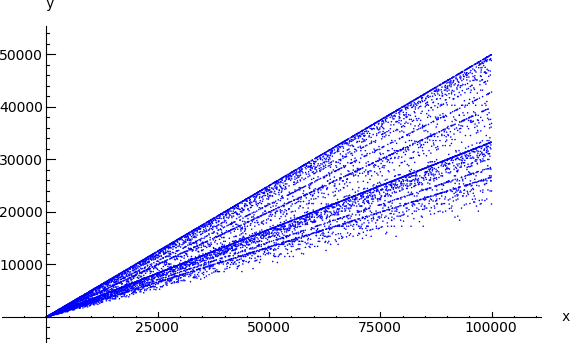
\includegraphics{figures/primitive-roots-all}
\caption{Die Anzahl der Primitivwurzeln f�r alle Primzahlen zwischen 1 und 100.000}
\label{fig:primitive_roots_all}
\end{figure}

\vskip +50 pt
Abbildung~\ref{fig:primitive_roots_smallest} gibt die kleinste Primitivwurzel
von jeder Primzahl zwischen 1 und 100.000 aus. Die $x$-Achse repr�sentiert
die Primzahlen 1 bis 100.000, die $y$-Achse gibt die kleinste Primitivwurzel
pro Primzahl aus.

\vskip +25 pt
Abbildung~\ref{fig:primitive_roots_largest} zeigt die entsprechende Graphik
mit der gr��ten Primitivwurzel zu jeder Primzahl im obigen Intervall.

\begin{figure}[!htbp]
\centering
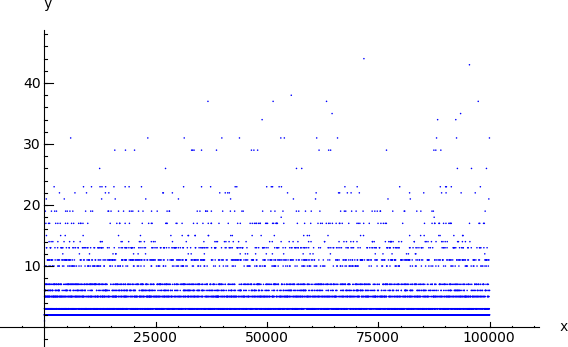
\includegraphics{figures/primitive-roots-smallest}
\caption{Die kleinste Primitivwurzel von jeder Primzahl zwischen 1 und 100.000}
\label{fig:primitive_roots_smallest}
\end{figure}

\begin{figure}[!htbp]
\centering
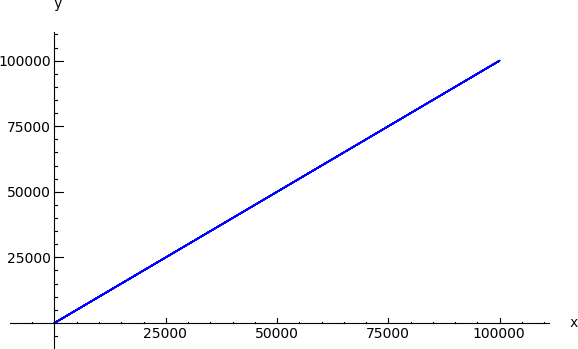
\includegraphics{figures/primitive-roots-largest}
\caption{Die gr��te Primitivwurzel von jeder Primzahl zwischen 1 und 100.000}
\label{fig:primitive_roots_largest}
\end{figure}

% To enforce that the next chapter starts at the beginning of a new page after
% the freely placed graphics, it was necessary to have TWO newpages and in between
% something to be printed (here invisible blanks).
% \newpage
% $ $
% I guess \clearpage is preferable.



% ---------------------------------------------------------------------------
\newpage
\hypertarget{NumberTheory_Sage_RSA sample}{}
\subsection{RSA-Beispiele mit Sage}
\label{l:NumberTheory_Sage_RSA sample}{}

\noindent In diesem Abschnitt sind die Sage-Quelltexte f�r die einfachen RSA-Beispiele
im Kapitel~\ref{rsaconcrete} (``\nameref{rsaconcrete}'') angegeben. 

\vskip +10 pt 
\hypertarget{AppArith4a}{%
\noindent \textbf{Beispiel auf Seite~\pageref{SrcArith4a}:}} \\
Die RSA-Exponentiation $M^{37} \pmod{3713}$ f�r die Nachricht $M = 120$ kann
mit Sage folgenderma�en ausgef�hrt werden:

\begin{Verbatim}%
[fontsize=\footnotesize,fontshape=tt]
sage: power_mod(120, 37, 3713)
1404
\end{Verbatim}


\vskip +10 pt 
\hypertarget{AppArith4b}{%
\noindent {\bf Beispiel auf Seite~\pageref{SrcArith4b}:}} \\

Die Faktorisierung von $J(256.027) = 255.016 = 2^3 * 127 * 251$ kann mit Sage
folgenderma�en durchgef�hrt werden:

\begin{sagecode}
\begin{Verbatim}%
[fontsize=\footnotesize,fontshape=tt]
sage: factor(255016)
2^3 * 127 * 251
\end{Verbatim}
\caption{Faktorisierung einer Zahl}
\end{sagecode}


\vskip +10 pt 
\hypertarget{AppArith4c}{%
\noindent {\bf Beispiel auf Seite~\pageref{SrcArith4c}:}} \\
RSA-Verschl�sselung mit Sage:

\begin{sagecode}
\begin{Verbatim}%
[fontsize=\footnotesize,fontshape=tt]
sage: A = [82, 83, 65, 32, 119, 111, 114, 107, 115, 33]
sage: e = 65537; m = 256027
sage: [power_mod(a, e, m) for a in A]
[212984, 25546, 104529, 31692, 248407, 100412, 54196, 100184, 58179, 227433]
\end{Verbatim}
\caption{RSA-Verschl�sselung durch modulare Exponentiation einer Zahl (als Nachricht)}
\end{sagecode}


\vskip +10 pt 
\hypertarget{AppArith4d}{%
\noindent {\bf Beispiel auf Seite~\pageref{SrcArith4d}:}} \\
RSA-Verschl�sselung mit Sage:

\begin{Verbatim}%
[fontsize=\footnotesize,fontshape=tt]
sage: A = [21075, 16672, 30575, 29291, 29473]
sage: e = 65537; m = 256027
sage: [power_mod(a, e, m) for a in A]
[158721, 137346, 37358, 240130, 112898]
\end{Verbatim}


\vskip +10 pt 
\hypertarget{AppArith4e}{%
\noindent {\bf Beispiel auf Seite~\pageref{SrcArith4e}:}} \\
RSA-Verschl�sselung mit Sage:

\begin{Verbatim}%
[fontsize=\footnotesize,fontshape=tt]
sage: A = [82083, 65032, 119111, 114107, 115033]
sage: e = 65537; m = 256027
sage: [power_mod(a, e, m) for a in A]
[198967, 51405, 254571, 115318, 14251]
\end{Verbatim}




% ---------------------------------------------------------------------------
\newpage
\hypertarget{NumberTheory_Sage_Number-of-RSA-keys}{}
\subsection{Wie viele RSA-Schl�ssel gibt es innerhalb eines Modulo-Bereiches?}
\label{l:NumberTheory_Sage_Number-of-RSA-keys}{}

Die RSA-Verschl�sselung wurde beschrieben in Abschnitt \ref{RSA} (``\nameref{RSA}'').
Schritt 1 bis 3 definieren die Schl�sselerzeugung, Schritt 4 und 5 stellen die
eigentliche Verschl�sselung dar:
\begin{itemize}
  \item[{\bf 1.}] W�hle zwei unterschiedliche Primzahlen $p$ and $q$
                  und berechne $n = p*q$.\\
                  Der Wert $n$ wird RSA-Modul genannt.

  \item[{\bf 2.}] W�hle ein zuf�lliges $e \in \{2, \cdots, n-1\}$, so dass gilt: \\
                  $e$ ist relativ prim zu $J(n) = (p-1)*(q-1)$. \\
                  Danach kann man $p$ und $q$ \glqq wegwerfen\grqq.

  \item[{\bf 3.}] W�hle $d \in \{1, \cdots, n-1\}$ mit $e*d \equiv 1  
                  {\rm ~(mod~} J(n))$,\\
		  d.h. $d$ ist die multiplikative Inverse von $e$ modulo $J(n)$.
		  Dann kann man $J(n)$ \glqq wegwerfen\grqq.
    \begin{itemize}
      \item[] $\rightarrow (n, e)$ ist der �ffentliche Schl�ssel $P$.
      \item[] $\rightarrow (n, d)$ ist der private Schl�ssel $S$ (nur $d$ muss man geheim halten).
    \end{itemize}

  \item[{\bf 4.}] Zur Verschl�sselung wird die Nachricht als (bin�re) Ziffernfolge
                  geschrieben. Diese Ziffernfolge wird dann so in gleich lange Teilfolgen
		  aufgeteilt, dass jede Teilfolge eine Zahl kleiner als $n$ darstellt.

  \item[{\bf 5.}] Vorgang der Verschl�sselung auf dem Klartext (bzw. auf Teilen davon)
                  $M \in \{1, \cdots, n-1\}$:
                  $$C = E ( (n, e); M ) := M^e {\rm ~(mod~} n).$$
\end{itemize}

Standardm��ig versucht man, einen mit RSA verschl�sselten Geheimtext $C$ dadurch zu knacken,
dass man den �ffentlichen Schl�ssel des Empf�ngers betrachtet und versucht, $n$ zu
faktorisieren. Hat man das erreicht, geht man wieder durch die Schritte 2 und 3 und
erzeugt den privaten Schl�ssel $e$, den man zum Entschl�sseln des Geheimtextes braucht.

Gem�� dem \glqq Primzahlsatz\grqq (beschrieben in Abschnitt \ref{thm-pz-pi-x}
\glqq \nameref{thm-pz-pi-x}\grqq) bewegt sich die Anzahl der Primzahlen
$PI(x)$ asymptotisch gegen  $x / ln(x)$.
F�r ein gegebenes $n$ gibt es also ca. $n / ln(n)$ m�gliche Werte f�r die
Primzahl $p$.

\noindent Will man nicht faktorisieren, sondern stellt sich eine Frage �hnlich
wie bei den klassischen Verschl�sselungsverfahren, kann man herausfinden wollen:
Wie viele verschiedene private Schl�ssel $(n, d)$ gibt es f�r einen bestimmten
Bereich der Schl�sselgr��e $n \in [a, b]$?

\noindent Das Sage-Beispielprogramm~\ref{nt_sagesample_Count_RSA_Keys} unten definiert
die Funktion \verb#count_Number_of_RSA_Keys#, die diese Frage konkret beantworten kann
(wenn der Modulus nicht zu gro� ist).\footnote{%
a) Der Aufruf \verb#sage: count_Number_of_RSA_Keys(100, 1000)# bedeutet, dass man
das Intervall $[100, 1000]$ f�r $n$ betrachtet.
$n$ war definiert durch die beiden Primzahlen $p, q: n = p*q$.
Daher kann eine Primzahl h�chstens den Wert $500$ annehmen, weil $2 * 500 =1000$.\\
Die Anzahl m�glicher Primzahl-Kombinationen betr�gt: $comb = 258$.\\
Die Anzahl der Primzahlen im gegebenen Bereich betr�gt: $143$.\\
Die Anzahl der privaten Schl�ssel betr�gt: $34.816$.

\noindent b) Der Aufruf \verb#sage: count_Number_of_RSA_Keys(100, 100, True)#
hat die folgende Ausgabe:\\
   - Number of private keys for modulus in a given range: 0\\
   - Number of primes in a given range: 0\\
   Der Grund daf�r ist, dass wir damit nur $n=100$ betrachten, und $100$ ist nicht
   semi-prim\index{Primzahl!semi-prim}\index{Primzahl!Halbprimzahl},
   d.h. $100$ ist nicht das Produkt von genau zwei Primzahlen.
}


\begin{sagecode}
\begin{Verbatim}%
[fontsize=\footnotesize,fontshape=tt]
def count_Number_of_RSA_Keys(start, end, Verbose=False):
      r"""
      How many private RSA keys (n,d) exist, if only modulus N is given, and start <= N <= end?
        (prime_range(u,o) delivers all primes >=u und < o).
      """
      a = start
      b = end
      s = 0
      comb = 0
      for p in prime_range(1, b/2+1):
          for q in prime_range(p + 1, b/2+1):
              if a <= p * q and p * q <= b:
                  comb = comb +1
                  s = s + (euler_phi(euler_phi(p * q))-1)
                  if Verbose:
                      print "p=%s, " % p + "q=%s, " % q + "s=%s" % s
      print "Number of private keys for modulus in a given range: %s" % s + " (comb=%s), " % comb

      # Just for comparison: How many primes are in this range?
      s = 0
      for p in prime_range(a, b+1):
          if Verbose:
              print "a=%s, " % a + "b=%s, " % b + "p=%s" % p
          s = s + 1
      print "Number of primes in a given range: %s" % s

print "\n\nDD_Start -- Testcases for count_Number_of_RSA_Keys(start, end)"
print "\n-----------Testcase: (100, 1000) [Should deliver 34.816]"
time count_Number_of_RSA_Keys(100, 1000)
print "\n-----------Testcase: (100, 107, True) [Should deliver 23]"
time count_Number_of_RSA_Keys(100, 107, True)
u = 10^3; o = 10^4;
print "\n-----------Testcase: (%s, " % u + "%s) [Should deliver 3.260.044]" % o
time count_Number_of_RSA_Keys(u, o)

OUTPUT:
DD_Start -- Testcases for count_Number_of_RSA_Keys(start, end)

-----------Testcase: (100, 1000) [Should deliver 34.816]
Number of private keys for modulus in a given range: 34816 (comb=258),
Number of primes in a given range: 143
Time: CPU 0.03 s, Wall: 0.04 s

-----------Testcase: (100, 107, True) [Should deliver 23]
p=2, q=53, s=23
Number of private keys for modulus in a given range: 23 (comb=1),
a=100, b=107, p=101
a=100, b=107, p=103
a=100, b=107, p=107
Number of primes in a given range: 3
Time: CPU 0.00 s, Wall: 0.00 s

-----------Testcase: (1000, 10000) [Should deliver 3.260.044]
Number of private keys for modulus in a given range: 3260044 (comb=2312),
Number of primes in a given range: 1061
Time: CPU 0.63 s, Wall: 0.66 s
\end{Verbatim}
\caption{Wie viele RSA-Schl�ssel gibt es, wenn man den Bereich f�r die Schl�sselgr��e n kennt?}
\label{nt_sagesample_Count_RSA_Keys}
\end{sagecode}

\noindent Weil es mehr private Schl�ssel $(n, d)$ innerhalb eines gr��eren
Bereiches von Werten f�r $n$ gibt, ist das Brute-force-Faktorisieren
viel effizienter als das Durchprobieren aller m�glichen Schl�ssel.




% ++++++++++++++++++++++++++++++++++++++++++++++++++++++++++++++++++++++++++
\clearpage
\newpage
\hypertarget{NumberTheory_Appendix_F}{}  %\hypertarget{AppendixListAndDef}{}
\section{Anhang: Liste der in diesem Kapitel formulierten Definitionen und S�tze}
\label{l:NumberTheory_Appendix_F}{}  %\label{l:AppendixListAndDef}{}

% \vskip +8 pt
\begin{center}
\begin{tabular}{|l|l|l|}\hline
 & Kurzbeschreibung~~ & Seite \\ \hline
Definition~\ref{def-zth-prime} & Primzahlen &  \pageref{def-zth-prime} \\
Definition~\ref{def-zth-composite} & Zusammengesetzte Zahlen
                                   & \pageref{def-zth-composite}  \\ \hline
Satz~\ref{thm-zth-cnum} & Teiler von zusammengesetzten Zahlen~~~~~~~ & \pageref{thm-zth-cnum}\\
Satz~\ref{thm-zth-mthm} &  Erster Hauptsatz der elementaren Zahlentheorie &  \pageref{thm-zth-mthm} \\  \hline
Definition~\ref{def-zth-divisibility} & Teilbarkeit & \pageref{def-zth-divisibility} \\
Definition~\ref{def-zth-remainder} & Restklasse $r$ modulo $m$ & \pageref{def-zth-remainder} \\
Definition~\ref{def-zth-congruence} & restgleich oder kongruent & \pageref{def-zth-congruence} \\ \hline
Satz~\ref{thm-zth-div} & Kongruenz mittels Differenz & \pageref{thm-zth-div} \\
Satz~\ref{thm-zth-multinv} & Multiplikative Inverse (Existenz) & \pageref{thm-zth-multinv}  \\
Satz~\ref{thm-zth-exhperm} & Ersch�pfende Permutation & \pageref{thm-zth-exhperm} \\
Satz~\ref{thm-zth-pot} & Gestaffelte Exponentiation mod $m$ & \pageref{thm-zth-pot} \\ \hline
Definition~\ref{def-zth-zn} & $\mathbb{Z}_n$  & \pageref{def-zth-zn}\\
Definition~\ref{def-zth-znmult} &   $\mathbb{Z}_n^*$ & \pageref{def-zth-znmult} \\ \hline
Satz~\ref{thm-zth-znmult} & Multiplikative Inverse in $\mathbb{Z}_n^*$& \pageref{thm-zth-znmult} \\ \hline
Definition~\ref{def-zth-phiofn} & Euler-Funktion $J(n)$ & \pageref{def-zth-phiofn} \\
Satz~\ref{thm-zth-phiprime} & $J(p)$ &  \pageref{thm-zth-phiprime}\\
Satz~\ref{thm-zth-phipq} & $J(p*q)$ &  \pageref{thm-zth-phipq}\\
Satz~\ref{thm-zth-phimultprime} & $J(p_1 * \cdots *p_k)$ & \pageref{thm-zth-phimultprime} \\
Satz~\ref{thm-zth-phinum} & $J(p_1^{e_1} * \cdots *p_k^{e_k})$ & \pageref{thm-zth-phinum} \\
Satz~\ref{thm-zth-fermat1} & Kleiner Satz von Fermat &  \pageref{thm-zth-fermat1}\\
Satz~\ref{thm-zth-fermateuler} & Satz von Euler-Fermat & \pageref{thm-zth-fermateuler} \\ \hline
Definition~\ref{def-zth-ordn} & Multiplikative Ordnung $ {\rm ord}_{m} (a)$ & \pageref{def-zth-ordn} \\
Definition~\ref{def-zth-primitiveroot} & Primitivwurzel von $m$ &  \pageref{def-zth-primitiveroot}\\
Satz~\ref{thm-zth-ordp} & Aussch�pfung des Wertebereiches & \pageref{thm-zth-ordp} \\ \hline
\end{tabular}
\end{center}
\vskip +6 pt





% ++++++++++++++++++++++++++++++++++++++++++++++++++++++++++++++++++++++++++
% ++++++++++++++++++++++++++++++++++++++++++++++++++++++++++++++++++++++++++
\newpage
%\addcontentsline{toc}{section}{Literaturverzeichnis}
\begin{thebibliography}{99999}
\addcontentsline{toc}{section}{Literaturverzeichnis}

\bibitem[Agrawal2002]{nt:Agrawal2002}  \index{Agrawal 2002} 
    M. Agrawal, N. Kayal, N. Saxena, \\
    {\em PRIMES in P}, August 2002, Korrigierte Fassung: \\
       \href{http://www.cse.iitk.ac.in/~manindra/algebra/primality_v6.pdf}
    {\texttt{http://www.cse.iitk.ac.in/~manindra/algebra/primality\_v6.pdf}} \\
    Siehe auch die Seite \glqq The AKS \glqq PRIMES in P'' Algorithm Resource'':
       \href{http://fatphil.org/maths/AKS/}
    {\texttt{http://fatphil.org/maths/AKS/}}

\bibitem[Bartholome1996]{nt:Bartholome1996} \index{Bartholome 1996}  
    A. Bartholom\'e, J. Rung, H. Kern, \\
    {\em Zahlentheorie f�r Einsteiger}, Vieweg 1995, 2. Auflage 1996.

\bibitem[Bauer1995]{nt:Bauer1995} \index{Bauer 1995}
    Friedrich L. Bauer, \\
    {\em Entzifferte Geheimnisse}, Springer, 1995.

\bibitem[Bauer2000]{nt:Bauer2000} \index{Bauer 2000}
    Friedrich L. Bauer, \\
    {\em Decrypted Secrets}, Springer 1997, 2nd edition 2000.

\bibitem[Bernstein2001]{nt:Bernstein2001} \index{Bernstein 2001}
    D.~J. Bernstein, \\
    {\em Circuits for integer factorization: a proposal},\\ 
    \href{http://cr.yp.to/papers/nfscircuit.ps}
    {\texttt{http://cr.yp.to/papers/nfscircuit.ps}} \\
    \href{http://cr.yp.to/djb.html}{\texttt{http://cr.yp.to/djb.html}}

\bibitem[Beutelspacher1996]{nt:Beutelspacher1996} \index{Beutelspacher 1996}
    Albrecht Beutelspacher, \\
    {\em Kryptologie}, Vieweg 1987, 5. Auflage 1996.

\bibitem[Bourseau2002]{nt:Bourseau2002} \index{Bourseau 2002} \index{Fox 2002}
    F. Bourseau, D. Fox, C. Thiel, \\
    {\em Vorz�ge und Grenzen des RSA-Verfahrens},\\
    In: Datenschutz und Datensicherheit (DuD) 26/2002, S. 84-89 (s. www.dud.de),
    \href{http://http://www.secorvo.de/publikationen/rsa-grenzen-fox-2002.pdf}
         {\texttt{http://www.secorvo.de/publikationen/rsa-grenzen-fox-2002.pdf}}

\bibitem[Brands2002]{nt:Brands2002} \index{Brands 2002}
    Gilbert Brands, \\
    {\em Verschl�sselungsalgorithmen -- Angewandte Zahlentheorie 
    rund um Sicherheitsprotokolle}, Vieweg, 2002.

\bibitem[BSI2002]{nt:BSI2002} \index{BSI 2002}
    BSI (Bundesamt f�r Sicherheit in der Informationstechnik), \\
    {\em Empfehlungen zur Wahl der Schl�ssell�ngen}, Bonn, 9.9.2002, \\
    (Geeignete Kryptoalgorithmen zur Erf�llung der Anforderungen
    nach \S 17 (1) SigG vom 22. Mai 2001 in Verbindung mit Anlage 1, 
    I 2, SigV vom 22. November 2001), \\
    \href{http://www.bsi.bund.de/esig/basics/techbas/krypto/bund02v7.pdf}
    {\tt http://www.bsi.bund.de/esig/basics/techbas/krypto/bund02v7.pdf} \\
    Eine Stellungnahme zu diesen Empfehlungen: \\
    \href{http://www.secorvo.de/publikat/stellungnahme-algorithmenempfehlung-020307.pdf}
    {\texttt{http://www.secorvo.de/publikat/}}\\
    \hspace*{1cm}
    \href{http://www.secorvo.de/publikat/stellungnahme-algorithmenempfehlung-020307.pdf}
    {\texttt{stellungnahme-algorithmenempfehlung-020307.pdf}}

\bibitem[Buchmann2004]{nt:Buchmann2004} \index{Buchmann 2004}
    Johannes Buchmann, \\
    {\em Einf�hrung in die Kryptographie}, Springer, 3. Auflage, 2004.

\bibitem[Buhler1993]{nt:Buhler1993} \index{Buhler 1993} 
    J.P. Buhler, H.W. Lenstra, C. Pomerance, \\
    {\em Factoring integers with the number field sieve}, \\
    In: A.K. Lenstra, H.W. Lenstra (Hrsg.): The Development of the 
    Number Field Sieve, Lecture Notes in Mathematics, Vol.~1554, 
    Springer, Heidelberg 1993, S. 50$-$94.

\bibitem[Eckert2003]{nt:Eckert2003} \index{Eckert 2003} 
    Claudia Eckert, \\
    {\em IT-Sicherheit: Konzepte-Verfahren-Protokolle}, 
    Oldenbourg 2001, 2. Auflage 2003.

\bibitem[Ertel2001]{nt:Ertel2001} \index{Ertel 2001} 
    Wolfgang Ertel, \\
    {\em Angewandte Kryptographie}, 
    Fachbuchverlag Leipzig FV 2001.

\bibitem[Graham1994]{nt:Graham1994} \index{Graham 1994}
     Graham, Knuth, Patashnik, \\
     {\em Concrete Mathemathics, a Foundation of Computer Science}, \\
     Addison Wesley 1989, 6th printing 1994.

\bibitem[Kippenhahn1997]{nt:Kippenhahn1997} \index{Kippenhahn 1997}
    Rudolph Kippenhahn, \\
    {\em Verschl�sselte Botschaften -- Geheimschrift, Enigma und Chipkarte}, 
    Rowohlt, 1997.

\bibitem[Kippenhahn1999]{nt:Kippenhahn1999} \index{Kippenhahn 1999}
    Rudolph Kippenhahn, \\
    {\em Code Breaking -- A History and Exploration}, 
    Constable, 1999.

\bibitem[Knuth1998]{nt:Knuth1998} \index{Knuth 1998}
    Donald E. Knuth, \\
    {\em The Art of Computer Programming, vol 2: Seminumerical Algorithms}, \\
    Addison-Wesley, 2nd edition 1998.
    % Wann war die erste Edition ?

\bibitem[Lenstra1993]{nt:Lenstra1993} \index{Lenstra 1993}
     A. Lenstra, H. Lenstra: \\ 
     {\em The development of the Number Field Sieve}, \\
     Lecture Notes in Mathematics 1554, Springer, New York 1993

\bibitem[Lenstra1999]{nt:Lenstra1999} Arjen K. Lenstra, Eric R. Verheul,
     \index{Lenstra/Verheul 1999} \\
     {\em Selecting Cryptographic Key Sizes (1999)}, \\
     Journal of Cryptology: the journal of the International 
     Association for Cryptologic Research \\
     \href{http://www.cryptosavvy.com/cryptosizes.pdf}
     {\texttt{http://www.cryptosavvy.com/cryptosizes.pdf}}

\bibitem[Lenstra2002]{nt:Lenstra2002} \index{Lenstra 2002}
    Arjen K. Lenstra, Adi Shamir, Jim Tomlinson, Eran Tromer,\\
    {\em Analysis of Bernstein's Factorization Circuit},\\
    \href{http://www.cryptosavvy.com/mesh.pdf}
    {\texttt{http://www.cryptosavvy.com/mesh.pdf}}

\bibitem[Menezes2001]{nt:Menezes2001} \index{Menezes 2001}
    Alfred J. Menezes, Paul C. van Oorschot, Scott A. Vanstone \\
    {\em Handbook of Applied Cryptography}, 
    CRC Press 1997, 5th printing 2001.

\bibitem[Pfleeger1997]{nt:Pfleeger1997} \index{Pfleeger 1997}
    Charles P. Pfleeger, \\
    {\em Security in Computing}, Prentice-Hall, 2nd edition 1997.
    % Im Buch stand nicht, wann die 1. Edition rauskam.

\bibitem[Pomerance1984]{nt:Pomerance1984} \index{Pomerance 1984} 
    C. Pomerance, \\
    {\em The quadratic sieve factoring algorithm}, \\
    In: G.R. Blakley, D. Chaum (Hrsg.): Proceedings of Crypto '84, 
    LNCS 196, Springer Berlin 1995, S. 169-182.

\bibitem[RSA Security 2002]{nt:RSA Security 2002} \index{RSA Security 2002} 
    RSA Security, \\
    {\em Has the RSA algorithm been compromised as a result 
    of Bernstein's Paper?}, \\
    8. April 2002, \\
    \href{http://www.rsasecurity.com/}{\tt http://www.rsasecurity.com/}.

\bibitem[SchneiderM2004]{nt:SchneiderM2004} \index{SchneiderM 2004} 
    Matthias Schneider, \\
    {\em Analyse der Sicherheit des RSA-Algorithmus. \\
     M�gliche Angriffe, deren Einfluss auf sichere Implementierungen
     und �konomische Konsequenzen}, \\
    Diplomarbeit an der Universit�t Siegen, 2004.

\bibitem[Schneier1996]{nt:Schneier1996nt} \index{Schneier 1996} 
    Bruce Schneier, \\
    {\em Applied Cryptography, Protocols, Algorithms, and Source Code in C}, \\
    Wiley and Sons 1994, 2nd edition 1996.

\bibitem[Schwenk2002]{nt:Schwenk2002}\index{Schwenk 2002}
    J�rg Schwenk, \\
    {\em Sicherheit und Kryptographie im Internet}, 
    Vieweg 2002.

\bibitem[Sedgewick1990]{nt:Sedgewick1990} \index{Sedgewick 1990}
    Robert Sedgewick,\\
    {\em Algorithms in C}, Addison-Wesley, 1990.

\bibitem[Shamir2003]{nt:Shamir2003} \index{Shamir 2003} \index{TWIRL-Device} 
    Adi Shamir, Eran Tromer, \\
    {\em Factoring Large Numbers with the TWIRL Device}, 
    Januar 2003, \\
    \href{http://www.wisdom.weizmann.ac.il/~tromer/}
    {\texttt{http://www.wisdom.weizmann.ac.il/\~{}tromer/}}

\bibitem[Shamir2003a]{nt:Shamir2003a} \index{Shamir 2003a} \index{TWIRL-Device} 
    Adi Shamir, Eran Tromer, \\
    {\em On the Cost of Factoring RSA-1024}, 
    RSA Laboratories CryptoBytes Volume 6, No. 2, Summer 2003, S. 11-20 \\
    \href{http://www.rsasecurity.com/rsalabs/cryptobytes/CryptoBytes_August_2003.pdf}
    {\texttt{http://www.rsasecurity.com/rsalabs/cryptobytes/CryptoBytes\_August\_2003.pdf}}
  
\bibitem[Silverman2000]{nt:Silverman2000} \index{Silverman 2000}
     Robert D. Silverman: \\ 
     {\em A Cost-Based Security Analysis of Symmetric and Asymmetric 
          Key Lengths} \\ 
     In: RSA Laboratories Bulletin, No. 13, April 2000, S. 1-22

\bibitem[Stinson1995]{nt:3Stinson1995} \index{Stinson 1995}
    Douglas R. Stinson,\\
    {\em Cryptography - Theory and Practice}, CRC Press, 1995.

\bibitem[Weis2003]{nt:Weis2003} \index{Weis 2003} \index{Lucks 2003} \index{Bogk 2003}
    R�diger Weis, Stefan Lucks, Andreas Bogk, \\
    {\em Sicherheit von 1024 bit RSA-Schl�sseln gef�hrdet},\\
    In: Datenschutz und Datensicherheit (DuD) 6/2003, S. 360-362 (s. www.dud.de)\\
    Der Artikel erl�utert Details zum TWIRL-Device\index{TWIRL-Device}.

\bibitem[Welschenbach2001]{nt:Welschenbach2001} \index{Welschenbach 2001}
    Welschenbach, Michael, \\
    {\em Kryptographie in C und C++}, Springer 2001.

\bibitem[Wiles1994]{nt:Wiles1994} \index{Wiles, Andrew}
    Wiles, Andrew, \\
    {\em Modular elliptic curves and Fermat's Last Theorem}%
    \index{Fermat!letzter Satz}, \\
    In: Annals of Mathematics 141 (1995).

\bibitem[Wolfenstetter1998]{nt:Wolfenstetter1998} \index{Wolfenstetter 1998}
    Albrecht Beutelspacher, J�rg Schwenk, Klaus-Dieter Wolfenstetter, \\
    {\em Moderne Verfahren in der Kryptographie}, 
    Vieweg 1995, 2. Auflage 1998.

\bibitem[Yan2000]{nt:Yan2000} \index{Yan 2000} 
    Song Y. Yan, \\
    {\em Number Theory for Computing}, Springer, 2000.
    
\end{thebibliography}



% ++++++++++++++++++++++++++++++++++++++++++++++++++++++++++++++++++++++++++
\newpage
\section*{Web-Links}\addcontentsline{toc}{section}{Web-Links}

\begin{enumerate}
   \item \hypertarget{knott}{} \index{Knott, Ron}
          Fibonacci-Seite \index{Fibonacci} von Ron Knott, \\
          Hier dreht sich alles um Fibonacci-Zahlen. \\
          \href{http://www.mcs.surrey.ac.uk/personal/R.Knott/Fibonacci/fib.html}
	  {\texttt{http://www.mcs.surrey.ac.uk/personal/R.Knott/Fibonacci/fib.html}}
          
   \item CrypTool,  \index{CrypTool} \\
          E-Learning-Freeware zur Veranschaulichung von Kryptographie
          und Kryptoanalyse, \\
          \href{http://www.cryptool.de}{\texttt{http://www.cryptool.de}}, \\
          \href{http://www.cryptool.org}{\texttt{http://www.cryptool.org}},\\ 
          \href{http://www.cryptool.com}{\texttt{http://www.cryptool.com}}
          
   \item Mathematica, \index{Mathematica} \\
          Kommerzielles Mathematik-Paket \\
          \href{http://www.wolfram.com}{\texttt{http://www.wolfram.com }}
          
   \item  LiDIA, \index{LiDIA} \\ 
          Umfangreiche Bibliothek mit zahlentheoretischen Funktionen und dem
          Interpreter LC \\
          \href{http://www.informatik.tu-darmstadt.de/TI/LiDIA}
          {\texttt{http://www.informatik.tu-darmstadt.de/TI/LiDIA}}
          
   \item BC, \index{BC} \\
         Interpreter mit zahlentheoretischen Funktionen \\
         \href{http://www.gnu.org/software/bc/bc.html}
         {\texttt{http://www.gnu.org/software/bc/bc.html}}
         %Check 11.5.07: nicht mehr zug�nglich.
         %\href{http://www.maths.uq.edu.au/~krm/gnubc.html}
         %{\texttt{http://www.maths.uq.edu.au/\~{}}krm/gnubc.html}
         
   \item Pari-GP, \index{Pari-GP} \\
         Hervorragender, schneller und freier Interpreter mit
         zahlentheoretischen Funktionen. \\ 
         \href{http://pari.math.u-bordeaux.fr/}
              {\texttt{http://pari.math.u-bordeaux.fr/}}\\
         \href{http://en.wikipedia.org/wiki/PARI/GP}
              {\texttt{http://en.wikipedia.org/wiki/PARI/GP}}\\
         Ressourcen zu PARI/GP auf der Webseite von Karim Belabas:\\
         \href{http://www.math.u-bordeaux.fr/~belabas/pari/}
              {\texttt{http://www.math.u-bordeaux.fr/\~{}belabas/pari/}}

   \item \index{Munchenbach@M�nchenbach, Carsten}
         Erst nach Vollendung dieses Artikels wurde mir die Web-Seite von
         Herrn M�nchenbach bekannt, die interaktiv und didaktisch sehr
         ausgereift die grundlegenden Denkweisen der Mathematik anhand
         der elementaren Zahlentheorie nahebringt. Sie entstand f�r
         ein Unterrichtsprojekt der 11. Klasse des Technischen Gymnasiums
         (leider nur in Deutsch verf�gbar): \\
         \href{http://www.hydrargyrum.de/kryptographie}
         {\texttt{http://www.hydrargyrum.de/kryptographie}}
         
   \item Seite des Beauftragten f�r die Lehrplanentwicklung des Fachs
         Informatik an der gymnasialen Oberstufe des Landes Saarland.
         Hier befindet sich eine Sammlung von Texten und Programmen 
         (in Java), die aus didaktischen �berlegungen entstand (alles 
         leider nur in Deutsch verf�gbar). \\
         \href{http://www.saar.de/~awa/kryptolo.htm}
         {\texttt{http://www.saar.de/\~{}awa/kryptolo.htm}}
         
   \item BSI, \index{BSI}\\ 
         Bundesamt f�r Sicherheit in der Informationstechnik \\
         \href{http://www.bsi.bund.de}{\texttt{http://www.bsi.bund.de}}

   \item Faktorisierungsrekorde und Challenges\index{Faktorisierung!Faktorisierungsrekorde},\\
         \href{http://www.crypto-world.com/}
           {\texttt{http://www.crypto-world.com/}} \\
         \href{http://www.crypto-world.com/FactorWorld.html}
           {\texttt{http://www.crypto-world.com/FactorWorld.html}}, Webseite von Scott Contini \\
         \href{http://www.loria.fr/~zimmerma/records/factor.html}
           {\texttt{http://www.loria.fr/\~{}zimmerma/records/factor.html}} \\
         \href{http://www.tutorgig.com/ed/RSA\_number}
           {\texttt{http://www.tutorgig.com/ed/RSA\_number}} \\

         \href{http://www.uni-bonn.de/Aktuelles/Pressemitteilungen/pm02/pm035-02.html}
           {\texttt{http://www.uni-bonn.de/Aktuelles/Pressemitteilungen/pm02/pm035-02.html}} \\
         \href{http://www.ercim.org/publication/Ercim\_News/enw49/franke.html, 2002-01}
           {\texttt{http://www.ercim.org/publication/Ercim\_News/enw49/franke.html, 2002-01}} \\
         \href{http://www.loria.fr/~zimmerma/records/rsa160}
           {\texttt{http://www.loria.fr/\~{}zimmerma/records/rsa160}} \\

         \href{http://www.rsa.com/rsalabs/node.asp?id=2092}
           {\texttt{http://www.rsa.com/rsalabs/node.asp?id=2092}}
	 
   \item Das Cunningham-Projekt, \index{Cunningham-Projekt}\\ 
         \href{http://www.cerias.purdue.edu/homes/ssw/cun/}
         {\texttt{http://www.cerias.purdue.edu/homes/ssw/cun/}}

   \item Sage, \index{Sage} \\
         Ausgezeichnetes Open-Source Computer-Algebra-System, basierend auf Python
	 als Skript-Sprache. Damit sind die Code-Beispiele in diesem Kapitel erstellt.
	 Vergleiche die Einf�hrung in Kapitel~\ref{s:appendix-using-sage}.\\
         \href{http://www.sagemath.org/}
              {\texttt{http://www.sagemath.org/}}\\
         \href{http://en.wikipedia.org/wiki/Sage_%28mathematics_software%29}
              {\texttt{http://en.wikipedia.org/wiki/Sage\_\%28mathematics\_software\%29}}\\

\end{enumerate}



% ++++++++++++++++++++++++++++++++++++++++++++++++++++++++++++++++++++++++++
\vskip +20 pt
\section*{Dank} \addcontentsline{toc}{section}{Dank}
Ich m�chte hier die Gelegenheit nutzen, den folgenden Personen ganz 
herzlich zu danken: 
\begin{itemize}

  \item {Hr. Henrik Koy f�r das anregende und sehr konstruktive 
         Korrekturlesen und f�r die vielen Verbesserungen der ersten
	 Version dieses Artikels, und f�r die Hilfen bei TeX, ohne die
	 dieser Artikel nie in dieser Form erschienen w�re. \\
	 Au�erdem hat Hr. Koy in seiner Freizeit im CrypTool-Programm 
	 die komplexe Dialogbox zum RSA-Kryptosystem
%	 RSA-Krypto"-system   (TRENNUNG erzwingen)
	 designed und die dahinterliegende Logik entwickelt, mit der die
	 RSA-Beispiele dieses Artikels nachvollzogen werden k�nnen.}

  \item {J�rg Cornelius Schneider f�r die engagierte Unterst�tzung bei TeX und
         die mannigfaltigen Hilfen bei allen Arten von Programmier- und
	 Design-Problemen.}

  \item {Dr. Georg Illies f�r den Hinweis auf Pari-GP\index{Pari-GP}.}
  
  \item {Lars Fischer f�r seine Hilfe bei schnellem Pari-GP\index{Pari-GP}-Code
         f�r Primitivwurzeln.}
  
  \item {Minh Van Nguyen aus Australien f�r seine immer schnelle, kompetente und
         ausf�hrliche Hilfe bei den Sage\index{Sage}-Code-Beispielen in diesem
	 Kapitel.}

\end{itemize}



% Local Variables:
% TeX-master: "../script-de.tex"
% End:

% $Id$
\setcounter{satz}{0}
\setcounter{definition}{0}

\newcommand{\NT}{\vspace*{0.2\baselineskip}\\}
\newcommand{\HZ}{\vspace*{0.5\baselineskip}}
\newcommand{\R}{\text{I}\!\text{R}}
\newcommand{\N}{\text{I}\!\text{N}}
\newcommand{\Q}{\text{Q}\!\!\!\text{l}\,\,}
\newcommand{\C}{\text{C}\!\!\!\text{l}\,\,}
\newcommand{\K}{\text{I}\!\text{K}}
\newcommand{\Z}{\mathbf{\mathbb{Z}}}
%--------------------------------------- matheScript-Zeichen definieren
\newcommand{\fs}{\mathscr{F}}  
\newcommand{\es}{\mathscr{E}}  
\newcommand{\cs}{\mathscr{C}}  
\newcommand{\gs}{\mathscr{G}}
\newcommand{\is}{\mathscr{I}}
\newcommand{\os}{\mathscr{O}}
\newcommand{\ks}{\mathscr{K}}
\newcommand{\qs}{\mathscr{Q}}
\newcommand{\us}{\mathscr{U}}
\newcommand{\hs}{\mathscr{H}}
\newcommand{\ps}{\mathscr{P}}
\newcommand{\as}{\mathscr{A}}
\newcommand{\rs}{\mathscr{R}}
\newcommand{\bs}{\mathscr{B}}
%-------------------------------------
\newcommand{\PG}{\text{I}\!\text{P}}
\newcommand{\carre}{\square}
\newcommand{\ncarre}{/\negthickspace\negthickspace\square}
\newcommand{\ncarreq}{{\ncarre}_q}
\newcommand{\ncarree}{/\negthickspace\negthickspace\negthickspace\square}
\newcommand{\ncarrepi}{{\ncarre}_{p^i}}
\newcommand{\mc}[1]{{\cal #1}}
\newcommand{\Char}{\text{char}}
\newcommand{\Aut}{\text{Aut}}
\newcommand{\Fix}{\text{Fix}}
\newcommand{\Syl}{\text{Syl}}
\newcommand{\Bild}{\text{Bild}}
\newcommand{\ggt}{\text{ggT}}
\newcommand{\kgv}{\text{kgV}}
\newcommand{\Id}{\text{Id}}
\newcommand{\nqcarre}{{\ncarre}_{q^2}}

\setlength{\fboxrule}{.4pt}
\setlength{\fboxsep}{4pt}

\newpage
%**************************************************************************************************************************
\section{Die mathematischen Ideen hinter der modernen Kryptographie}
%**************************************************************************************************************************
(Oyono R./ Esslinger B., Sep. 2000, Updates Nov. 2000, Feb. 2003)
%--------------------------------------------------------------------------------------------------------------------------
       \subsection{Einwegfunktionen mit Fallt"ur und Komplexit"atsklassen}
%--------------------------------------------------------------------------------------------------------------------------
\index{Kryptographie!moderne} \index{Einwegfunktion}
Eine {\bf Einwegfunktion} \hypertarget{Einwegfunktionen1}{} ist eine effizient zu 
berechnende (injektive) Funktion, deren Umkehrung jedoch nur mit 
extrem hohem Rechenaufwand -- jedoch praktisch unm"oglich -- zu berechnen ist.\par

Etwas genauer formuliert:  Eine Einwegfunktion ist eine Abbildung $ f $ einer Menge $ X $ in eine Menge $ Y, $ so dass $ f(x) $ f"ur jedes Element $ x $ von $ X $ leicht zu berechnen ist, w"ahrend es f"ur (fast) jedes $ y $ aus $ Y $  praktisch unm"oglich ist, ein Urbild $ x $ (d.h. ein $ x $ mit $ f(x)=y $) zu finden.\par

Ein allt"agliches Beispiel f"ur eine Einwegfunktion ist ein Telefonbuch: die auszuf"uhrende Funktion ist die, einem Namen die entsprechende Telefonnummer zuzuordnen. Da die Namen alphabetisch geordnet sind, ist diese Zuordnung einfach auszuf"uhren. Aber ihre Invertierung, also die Zuordnung eines Namens zu einer gegebenen Nummer, ist offensichtlich schwierig, wenn man nur ein Telefonbuch zur Verf"ugung hat. \par

Einwegfunktionen spielen in der Kryptographie eine entscheidende Rolle. Fast alle kryptographischen Begriffe kann man durch Verwendung des Begriffs Einwegfunktion umformulieren. Als Beispiel betrachten wir die Public Key-Verschl"usselung \index{Verschl""usselung!Public Key} (asymmetrische Kryptographie):\par

Jedem Teilnehmer $ T $ des Systems wird ein privater \index{Schl""ussel!privat}
\index{Schl""ussel!""offentlich} Schl"ussel $d_T$~\mbox{und} ein sogenannter "offentlicher Schl"ussel $ e_T $   zugeordnet. Dabei muss die folgende Eigenschaft (Public Key-Eigenschaft) gelten:\\
F"ur einen Gegner, der den "offentlichen Schl"ussel $ e_T $  kennt, ist es praktisch unm"oglich, den privaten Schl"ussel  $ d_T $ zu bestimmen.\par

Zur Konstruktion n"utzlicher Public Key-Verfahren sucht man also eine Einwegfunktion, die in einer Richtung \glqq einfach\grqq {} zu berechnen, die in der anderen Richtung jedoch \glqq schwer\grqq {} (praktisch unm"oglich) zu berechnen ist, solange eine bestimmte zus"atzliche Information \index{Einwegfunktion!mit Fallt""ur} (Fallt"ur) nicht zur Verf"ugung steht. Mit der zus"atzlichen Information kann die Umkehrung effizient gel"ost werden. Solche Funktionen nennt man {\bf Einwegfunktionen mit Fallt"ur} (trapdoor one-way function). Im obigen Fall ist $ d_T $ die Fallt"ur-In"-for"-ma"-tion. \par

Dabei bezeichnet man ein Problem als \glqq einfach\grqq, wenn es in \index{Laufzeit!polynomial} polynomialer Zeit als Funktion der L"ange der Eingabe l"osbar ist, d.h. wenn es so gel"ost werden kann, dass der Zeitaufwand sich als polynomiale Funktion in Abh"angigkeit der L"ange der Eingabe darstellen l"�sst. 
Wenn die L"ange der Eingabe $ n $ Bits betr"agt, so ist die Zeit der Berechnung der Funktion proportional zu $ n^{a}, $ wobei $ a $  eine Konstante ist. Man sagt, dass die \index{Komplexit""at} Komplexit"at solcher Probleme $ O(n^{a}) $ betr"agt (Landau- oder Big-O-Notation). 

Vergleicht man 2 Funktionen  $ 2^n $  und   $ n^{a} $, wobei $ a $  
eine Konstante ist, dann gibt es immer einen Wert f"ur  $ n $, ab dem
f"ur alle weiteren $ n $ gilt: $ n^{a}  <  2^n $. 
Die Funktion  $ n^{a} $  hat eine geringere Komplexit"at.
Z.B. f"ur $ a=5 $ gilt: ab der L"ange $ n=23 $ ist 
$ 2^n > n^5 $ ~\mbox{und} danach w"achst $ 2^n $ auch deutlich 
schneller \
[($ 2^{22}= 4.194.304 $, $ 22^5= 5.153.632 $); \
 ($ 2^{23}= 8.388.608 $, $ 23^5= 6.436.343 $); \
 ($ 2^{24}=16.777.216 $, $ 24^5= 7.962.624 $);].\par 
% "\mbox" nur, weil bei Ausdruck bei be die Blanks stets falsch sa�en:
%  "n^5un d"

Der Begriff \glqq praktisch unm"oglich\grqq {} ist etwas schwammiger. 
Allgemein kann man sagen, ein Problem ist \index{Laufzeit!effizient}
nicht effizient l"osbar, wenn der zu seiner L"osung ben"otigte Aufwand
schneller w"achst als die polynomiale Zeit als Funktion der Gr"o"se der
Eingabe. Wenn beispielsweise die L"ange der Eingabe $ n $  Bits betr"agt
und die Zeit zur Berechnung der Funktion proportional zu $ 2^n $ ist, 
so gilt gegenw"artig: die Funktion ist f"ur $n > 80$ praktisch nicht zu 
berechnen.

Die Entwicklung eines praktisch einsetzbaren Public Key-Verfahrens h"angt daher von der Entdeckung einer geeigneten Einwegfunktion mit Fallt"ur ab.\par

Um Ordnung in die verwirrende Vielfalt von m"oglichen Problemen und ihre Komplexit"aten zu bringen, fasst man Probleme mit "ahnlicher Komplexit"at zu Klassen zusammen.

Die wichtigsten Komplexit"atsklassen  sind die Klassen \textbf{P} und \textbf{NP}: 

\begin{itemize}

    \item Die Klasse \textbf{P}: Zu dieser Klasse geh"oren diejenigen Probleme, die mit polynomialem Zeitaufwand l"osbar sind.
    
    \item Die Klasse \textbf{NP}: Bei der Definition dieser Klasse betrachten wir nicht den Aufwand zur L"osung eines Problems, sondern den Aufwand zur Verifizierung einer gegebenen L"osung. Die Klasse \textbf{NP} besteht aus denjenigen Problemen, bei denen die Verifizierung einer gegebenen L"osung mit polynomialem Zeitaufwand m"oglich ist. Dabei bedeutet der Begriff \textbf{NP} \glqq nichtdeterministisch\grqq {} polynomial und bezieht sich auf ein Berechnungsmodell, d.h. auf einen nur in der Theorie existierenden Computer, der richtige L"osungen nichtdeterministisch \glqq raten\grqq {} und dies dann in polynomialer Zeit verifizieren kann.

\end{itemize}

Die Klasse \textbf{P} ist in der Klasse \textbf{NP} enthalten. Ein ber"uhmtes offenes Problem ist die Frage, ob $ \textbf{P} \neq \textbf{NP} $ gilt oder nicht, d.h. ob \textbf{P} eine echte Teilmenge ist oder nicht. Eine wichtige Eigenschaft der Klasse \textbf{NP} ist, dass sie auch sogenannte \glqq \textbf{NP}-vollst"andige\grqq {} Probleme enth"alt. Dies sind Probleme, welche die Klasse \textbf{NP} im folgenden Sinne vollst"andig repr"asentieren: Wenn es einen \glqq guten\grqq {} Algorithmus f"ur ein solches Problem gibt, dann existieren f"ur alle Probleme aus \textbf{NP} \glqq gute\grqq {} Algorithmen. Insbesondere gilt: wenn auch nur ein vollst"andiges Problem in \textbf{P} l"age, d.h. wenn es einen polynomialen L"osungsalgorithmus f"ur dieses Problem g"abe, so w"are \textbf{P}=\textbf{NP}. In diesem Sinn sind die \textbf{NP}-vollst"andigen Probleme die schwierigsten Probleme in \textbf{NP}.

Viele kryptographische Protokolle sind so gemacht, dass die \glqq guten\grqq {} Teilnehmer nur Probleme aus \textbf{P} l"osen m"ussen, w"ahrend sich ein Angreifer vor Probleme aus \textbf{NP} gestellt sieht.

Man wei"s leider bis heute nicht, ob es Einwegfunktionen "uberhaupt gibt. Man kann aber zeigen, dass Einwegfunktionen genau dann existieren, wenn $ \textbf{P} \neq \textbf{NP} $ gilt \cite[S.63]{Balcazar1988}.
\vskip +5pt

Es gab immer wieder die Aussage, jemand habe die "Aquivalenz bewiesen, z.B.

\href{http://www.geocities.com/st\_busygin/clipat.html}{\texttt{http://www.geocities.com/st\_busygin/clipat.html}}, 

aber bisher erwiesen sich diese Aussagen stets als falsch.

Es wurden eine Reihe von Algorithmen f"ur Public Key-Verfahren vorgeschlagen. Einige davon erwiesen sich, obwohl sie zun"achst vielversprechend erschienen, als polynomial l"osbar. Der ber"uhmteste durchgefallene Bewerber ist der Knapsack mit Fallt"ur, der von Ralph Merkle \cite{Merkle1978} vorgeschlagen wurde.


\newpage
%--------------------------------------------------------------------
       \subsection{Knapsackproblem als Basis f"ur Public Key-Verfahren} \index{Kryptographie!Public Key}
%--------------------------------------------------------------------
%--------------------------------------------------------------------
    \subsubsection{Knapsackproblem} \index{Knapsack}

%--------------------------------------------------------------------

Gegeben $ n $ Gegenst"ande $ G_1, \dots, G_n $ mit den Gewichten $ g_1, \dots g_n $ und den Werten $w_1, \cdots, w_n. $ Man soll wertm"a"sig so viel wie m"oglich unter Beachtung einer oberen Gewichtsschranke $ g $ davontragen. Gesucht ist also eine Teilmenge von $ \{ G_1, \cdots,G_n\}, $ etwa $ \{G_{i_1}, \dots ,G_{i_k} \}, $ so dass  $ w_{i_1}+ \cdots +w_{i_k} $ maximal wird unter der Bedingung $  g_{i_1}+ \cdots +g_{i_k} \leq g. $ \par
Derartige Fragen sind sogenannte {\bf NP}-vollst"andige Probleme (nicht \index{Laufzeit!nicht polynomial NP} deterministisch polynomial), die aufwendig zu berechnen sind.\index{Knapsack}

Ein Spezialfall des Knapsackproblems ist:\\
Gegeben sind die nat"urlichen Zahlen $ a_1, \dots, a_n $   und $ g .$
Gesucht sind  $ x_1, \dots, x_n \in \{ 0,1\} $  mit $ g = \sum_{i=1}^{n}x_i a_i $  (wo also $ g_i = a_i = w_i $ gew"ahlt ist).
Dieses Problem hei"st auch  {\bf 0-1-Knapsackproblem} und wird mit $ K(a_1, \dots, a_n;g) $  bezeichnet.\\

Zwei 0-1-Knapsackprobleme  $ K(a_1, \dots, a_n;g) $   und  $ K(a'_1, \dots, a'_n;g') $  hei"sen kongruent, falls es zwei \index{teilerfremd} teilerfremde Zahlen $ w $ und $ m $ gibt, so dass
\begin{enumerate}
    \item $ m > \max \{ \sum_{i=1}^n a_i , \sum_{i=1}^n a'_i \}, $

    \item $ g \equiv wg' \mod m, $

    \item $ a_i \equiv w a'_i \mod m $ f"ur alle $ i=1, \dots, n.$

\end{enumerate}
 
{\bf Bemerkung:}
Kongruente 0-1-Knapsackprobleme haben dieselben L"osungen.
Ein schneller Algorithmus zur Kl"arung der Frage, ob zwei 0-1-Knapsackprobleme kongruent sind, ist nicht bekannt.

Das L"osen eines 0-1-Knapsackproblems kann durch Probieren der $ 2^n $   M"oglichkeiten f"ur $ x_1, \dots, x_n $   erfolgen. Die beste Methode erfordert $ O(2^{n/2}) $  Operationen, was f"ur $ n=100 $  mit $ 2^{100} \approx 1,27 \cdot 10^{30} $  und  $ 2^{n/2} \approx 1,13 \cdot 10^{15} $ f"ur Computer eine un"uberwindbare H"urde darstellt.
Allerdings ist die L"osung f"ur spezielle $ a_1, \dots, a_n $   recht einfach zu finden, etwa f"ur $ a_i = 2^{i-1}. $  Die bin"are Darstellung von $ g $ liefert unmittelbar $ x_1, \dots, x_n$. Allgemein ist die L"osung des 0-1-Knapsackproblems leicht zu finden, falls eine \index{Permutation} Permutation\footnote{Eine Permutation\index{Permutation} $\pi$ der Zahlen $1, \dots, n$ ist die Vertauschung der Reihenfolge, in der
diese Zahlen aufgez"ahlt werden. Beispielsweise ist eine Permutation $\pi$ von $(1,2,3)$ gleich $(3,1,2),$ also $\pi(1) = 3$, $\pi(2) =1$ 
und $\pi(3) = 2$.} 
$ \pi $  von $ 1, \dots, n $  mit $ a_{\pi (j)} > \sum_{i=1}^{j-1} a_{\pi(i)} $  existiert. Ist zus"atzlich $ \pi $ die Identit"at, d.h. $ \pi(i)=i $ f"ur $ i=1,2,\dots,n, $ so hei"st die Folge $ a_1, \dots , a_n $ superwachsend.
Der folgende Algorithmus l"ost das Knapsackproblem mit superwachsender Folge im Zeitraum von $ O(n). $
\newpage
\begin{center}

\fbox{\parbox{12cm}{        
\begin{tabbing}
\hspace*{0.5cm} \= \hspace*{0.5cm} \= \hspace*{0.5cm} \= \kill
\>{\bf for} $ i=n $ {\bf to} 1 {\bf do} \\
\>\> {\bf if} $ T\geq a_i $ {\bf then}\\
\>\> \> $ T:=T-s_i $ \\
\>\>\> $ x_i:=1 $ \\
\>\> {\bf else} \\
\>\>\> $ x_i:=0 $\\
\>{\bf if} $ T=0 $ {\bf then} \\
\>\> $ X:=(x_1, \dots, x_n) $ ist die L"osung. \\
\>{\bf else} \\
\>\> Es gibt keine L"osung.
\end{tabbing}
}}
\end{center}
\vskip +10 pt
{\bf Algorithmus 1.} L"osen von Knapsackproblemen mit superwachsenden Gewichten
\vskip +20 pt


%--------------------------------------------------------------------
\subsubsection{Merkle-Hellman Knapsack-Verschl"usselung}
%--------------------------------------------------------------------
\index{Hellman Martin} \index{Merkle Ralph} 

1978 gaben Merkle und Hellman \cite{Merkle1978} \index{Verschl""usselung!Merkle-Hellman} ein Public Key-Verschl"usselungs-Verfahren an, das darauf beruht, das leichte 0-1-Knapsackproblem mit einer superwachsenden Folge in ein kongruentes mit einer nicht superwachsenden Folge zu \glqq verfremden\grqq. Es ist eine Blockchiffrierung, die bei jedem Durchgang einen $n$ Bit langen Klartext chiffriert.
\index{Knapsack!Merkle-Hellman}
Genauer:
\newpage

\begin{center}
\fbox{\parbox{12cm}{        
Es sei $ (a_1, \dots, a_n) $ superwachsend. Seien $ m $ und $ w $ zwei teilerfremde Zahlen mit $ m > \sum_{i=1}^{n} a_i $ und $ 1\leq w \leq m-1. $ W"ahle $\bar{w} $ mit $ w \bar{w} \equiv 1 \mod m $ die modulare Inverse von $ w $ und setze $ b_i:= wa_i \mod m, $ $ 0\leq b_i < m $ f"ur $ i=1, \dots ,n, $ und pr"ufe, ob die Folge $ b_1, \dots b_n $ nicht superwachsend ist. Danach wird eine Permutation $ b_{\pi (1)}, \dots , b_{\pi(n)} $ von $ b_1, \dots , b_n $ publiziert und insgeheim die zu $ \pi $ inverse Permutation $ \mu $ festgehalten. Ein Sender schreibt seine Nachricht in Bl"ocke $ (x_1^{(j)}, \dots, x_n^{(j)}) $ von Bin"arzahlen der L"ange $ n $ und bildet
\[ g^{(j)}:= \sum_{i=1}^n x_{i}^{(j)} b_{\pi(i)} \]
und sendet $ g^{(j)}, (j=1,2, \dots). $\par
Der Schl"usselinhaber bildet
\[ G^{(j)}:=\bar{w} g^{(j)} \mod m ,\quad 0 \leq G^{(j)} < m \]
und verschafft sich die $ x_{\mu(i)}^{(j)} \in \{ 0,1\} $ (und somit auch die $ x_i^{(j)} $) aus
\begin{eqnarray*}
G^{(j)} & \equiv & \bar{w} g^{(j)} = \sum_{i=1}^n x_i^{(j)} b_{\pi (i)} \bar{w} \equiv \sum_{i=1}^n x_i^{(j)} a_{\pi (i)} \mod m \\
& = & \sum_{i=1}^n x_{\mu (i)}^{(j)} a_{\pi (\mu (i))} = \sum _{i=1}^n x_{\mu (i)}^{(j)} a_i \mod m, 
\end{eqnarray*}
indem er die leichten 0-1-Knapsackprobleme $ K(a_1,\dots,a_n;G^{(j)}) $ mit superwachsender Folge $ a_1, \dots,a_n $ l"ost.
}}
\end{center}
\vskip +10 pt
{\bf Merkle-Hellman Verfahren} (auf Knapsackproblemen basierend).
\vskip +20 pt



1982 gab \index{Shamir Adi} Shamir \cite{Shamir1982} einen Algorithmus zum
Brechen des Systems in polynomialer Zeit an, ohne das allgemeine
Knapsackproblem zu l"osen. Len \index{Adleman Leonard} Adleman
\cite{Adleman1982} und Jeff Lagarias \index{Lagarias Jeff}
\cite{Lagarias1983} gaben einen Algorithmus zum Brechen des 2-fachen
iterierten Merkle-Hellman Knapsack-Verschl"usselungsverfahrens in
polynomialer Zeit an. Ernst Brickell \index{Brickell Ernst}
\cite{Brickell1985} gab schlie"slich einen Algorithmus zum Brechen des
mehrfachen iterierten Merkle-Hellman Knapsack-Verschl"usselungsverfahren in
polynomialer Zeit an. Damit war dieses Verfahren als
Verschl"usselungsverfahren ungeeignet. Dieses Verfahren liefert also eine
Einwegfunktion, deren Fallt"ur-In"-for"-ma"-tion (Verfremden des
0-1-Knapsackproblems) durch einen Gegner entdeckt werden k"onnte.


%---------------------------------------------------------------------
\subsection{Primfaktorzerlegung als Basis f"ur Public Key-Verfahren}\index{Primfaktor!Zerlegung}
%--------------------------------------------------------------------


%--------------------------------------------------------------------
\subsubsection[Das RSA-Verfahren]
{Das RSA-Verfahren\footnotemark}
\footnotetext{%
Mit CrypTool\index{CrypTool} v1.3 k"onnen Sie praktische Erfahrungen
mit dem RSA-Verfahren sammeln: per Men"u {\bf Einzelverfahren 
\textbackslash{} RSA-Demo \textbackslash{} RSA-Kryptosystem}.
}\index{RSA} \hypertarget{RSAVerfahren}{} 

Bereits 1978 stellten R. \index{Rivest Ronald} Rivest, \index{Shamir Adi} A. Shamir,  \index{Adleman Leonard} L. Adleman \cite{RSA1978} das bis heute wichtigste 
asymmetrische Kryptographie-Verfahren vor.  \par

\index{Faktorisierung!Faktorisierungsproblem}
\index{Eulersche Phi-Funktion}
\begin{center}
\fbox{\parbox{12cm}{        
\underline{Schl"usselgenerierung:} \vskip + 5pt
Seien $p$ und $q$ zwei verschiedene Primzahlen und $N=pq.$ Sei $e$ eine frei w"ahlbare, zu $ \phi (N) $ \index{Primzahl!relative} relative Primzahl, d.h. $ \ggt (e,\phi (N))=1. $ Mit dem Euklidschen Algorithmus berechnet man die nat"urliche Zahl  $ d < \phi (N), $ so dass gilt

\[ ed \equiv 1 \mod \phi (N). \]
Dabei ist $ \phi $ die {\bf Eulersche Phi-Funktion}. 

Der Ausgangstext wird in Bl"ocke zerlegt und verschl"usselt, wobei jeder Block einen bin"aren Wert $ x^{(j)} \leq N $ hat. \vskip + 5 pt

\underline{"Offentlicher Schl"ussel:}
\[ N,e. \]
\underline{Privater Schl"ussel:}
\[ d. \]
\underline{Verschl"usselung:}
\[ y= e_{T} (x) = x^{e} \mod N.\]
\underline{Entschl"usselung:}
\[ d_{T} (y) = y^d \mod N \]
}}
\end{center}

\vskip +10 pt
{\bf RSA-Verfahren} (auf dem Faktorisierungsproblem basierend).
\vskip +20 pt

{\bf Bemerkung:} 
Die Eulersche Phi-Funktion ist definiert duch: $ \phi (N)$ ist die  Anzahl der zu $ N $ \index{teilerfremd} {} teilerfremden nat"urlichen Zahlen 
$ x \leq N. $ Zwei nat"urliche Zahlen $ a $ und $ b $ \index{teilerfremd} sind teilerfremd, falls $ \ggt (a,b)=1. $ 

F"ur die Eulersche Phi-Funktion gilt: $ \phi (1)=1,~\phi(2)=1,
~\phi(3)=2, ~\phi (4)=2, ~\phi(6)=2, ~\phi (10)= 4, ~\phi (15)=8. $

Zum Beispiel ist $ \phi (24)=8, $ weil 
$|\{ x <24 : \ggt (x,24) =1 \}| =|\{1,5,7,11,13,17,19,23\}|. $

Ist  $ p $ eine Primzahl, so gilt $ \phi (p)= p-1. $

Kennt man die verschiedenen Primfaktoren  $ p_1, \dots , p_k $ von $ N, $ so ist $ \phi (N) = N \cdot (1-\frac{1}{p_1}) \,
\cdots \, (1-\frac{1}{p_k}) $\footnote{Weitere Formeln finden sich in den
Artikel \hyperlink{Kapitel_3_8}{\glqq Einf"uhrung in die elementare Zahlentheorie
mit Beispielen\grqq, Kap. 3.8}.}.

Im Spezialfall $ N=pq $ ist $ \phi (N)= pq(1-1/p)(1-1/q) = p(1-1/p)q(1-1/q)=(p-1)(q-1).$
\\ \vskip +5 pt
\begin{center}
\begin{tabular}{|l|l|l|}\hline
$n$ & $\phi (n) $ & Die zu $ n $ teilerfremden nat"urlichen Zahlen kleiner $ n. $ \\ \hline
1 & 1 & 1  \\
2 & 1 & 1 \\
3 &  2 & 1, 2 \\ 
4 &  2 & 1, 3 \\ 
5 &  4 & 1, 2, 3, 4 \\ 
6 &  2 & 1, 5 \\ 
7 &  6 & 1, 2, 3, 4, 5, 6 \\ 
8 &  4 & 1, 3, 5, 7 \\ 
9 &  6 & 1, 2, 4, 5, 7, 8 \\ 
10 &  4 & 1, 3, 7, 9 \\ 
15 &  8 & 1, 2, 4, 7, 8, 11, 13, 14 \\ \hline
\end{tabular}
\end{center}
\vskip +5 pt 
Die Funktion $ e_T $  ist eine Einwegfunktion, deren Fallt"ur-Information die Primfaktorzerlegung von $ N $ ist.

Zur Zeit ist kein Algorithmus bekannt, der das Produkt zweier Primzahlen bei sehr gro"sen Werten geeignet schnell
zerlegen kann (z.B. bei mehreren hundert Dezimalstellen). Die heute schnellsten bekannten Algorithmen \cite{Stinson1995} zerlegen eine 
zusammengesetzte ganze Zahl $ N $ in einem Zeitraum proportional zu  
$ L(N)= e^{\sqrt{\ln (N) \ln (\ln (N))}}. $ 
\vskip +5 pt
\begin{center}
\begin{tabular}{|l||l|l|l|l|l|l|}\hline
$N$ & $ 10^{50} $ & $ 10^{100} $ & $ 10^{150} $ & $ 10^{200} $ & $ 10^{250} $ & $ 10^{300} $ \\ \hline
$L(N)$ & $ 1,42 \cdot 10^{10} $ &  $ 2,34  \cdot 10^{15} $ &  $ 3,26 \cdot 10^{19} $ &  $ 1,20 \cdot 10^{23} $ &  $ 1,86 \cdot 10^{26} $ &  $ 1,53 \cdot 10^{29} $ \\ \hline
\end{tabular}
\end{center}
\vskip +5 pt 
Solange kein besserer Algorithmus gefunden wird, hei"st dies, dass Werte der
Gr"o"senordnung $ 100 $ bis $ 200 $ Dezimalstellen zur Zeit sicher sind.
Einsch"atzungen der aktuellen Computertechnik besagen, dass eine Zahl mit $100$
Dezimalstellen bei vertretbaren Kosten in etwa zwei Wochen zerlegt werden
k"onnte. Mit einer teuren Konfiguration (z.B. im Bereich von 10 Millionen
US-Dollar) k"onnte eine Zahl mit $150$ Dezimalstellen in etwa einem Jahr zerlegt
werden.  Eine $200-$stellige Zahl d"urfte noch f"ur eine sehr lange Zeit
unzerlegbar bleiben, falls es zu keinem mathematischen Durchbruch kommt. Zum
Beispiel w"urde es etwa 1000 Jahre dauern, um eine 200-stellige Zahl mit den
bestehenden Algorithmen in Primfaktoren zu zerlegen; dies gilt selbst dann, wenn
$ 10^{12} $  Operationen pro Sekunde ausgef"uhrt werden k"onnten, was jenseits
der Leistung der heutigen Technik liegt und in der Entwicklung Milliarden von
Dollar kosten w"urde. Dass es aber nicht doch schon morgen zu einem
mathematischen Durchbruch kommt, kann man nie ausschlie"sen.

Bewiesen ist bis heute nicht, dass das Problem, RSA zu brechen "aquivalent zum
Faktorisierungsproblem \index{Faktorisierung!Faktorisierungsproblem} ist. Es ist
aber klar, dass wenn das Faktorisierungsproblem \glqq gel"ost\grqq {} ist, dass
dann das RSA-Verfahren nicht mehr sicher ist.


%--------------------------------------------------------------------
    \subsubsection{Rabin-Public Key-Verfahren (1979)}
%--------------------------------------------------------------------

F"ur \index{Rabin} \index{Rabin!Public Key} dieses Verfahren konnte gezeigt werden, dass es "aquivalent zum Brechen des Faktorisierungsproblems ist. Leider ist dieses Verfahren anf"allig gegen chosen-ciphertext-Angriffe.
\index{Angriff!Chosen-ciphertext}
\begin{center}
\fbox{\parbox{12cm}{        
Seien $ p $ und $ q $ zwei verschiedene Primzahlen mit $ p,q\equiv 3 \mod 4 $ und $ n = pq.$ Sei $ 0\leq B \leq n-1.$ \\
\underline{"Offentlicher Schl"ussel:}
\[ e=(n,B). \]
\underline{Privater Schl"ussel:}
\[ d=(p,q). \]
\underline{Verschl"usselung:}
\[ y= e_{T} (x) = x(x+B) \mod n.\]
\underline{Entschl"usselung:}
\[ d_{T} (y) = \sqrt{y + B^2/4} -B/2 \mod n. \]
}}
\end{center}

\vskip +10 pt
{\bf Rabin-Verfahren} (auf dem Faktorisierungsproblem basierend).
\vskip +20 pt

Vorsicht:
Wegen $ p,q \equiv 3 \mod 4 $  ist die Verschl"usselung (mit Kenntnis des Schl"ussels) leicht  zu berechnen. Dies ist nicht der Fall f"ur $ p \equiv 1 \mod 4. $ Au"serdem ist die Verschl"usselungsfunktion nicht injektiv: Es gibt genau vier verschiedene Quellcodes, die $ e_T(x) $  als Urbild besitzen $ x,-x-B,\omega (x+B/2)-B/2, -\omega(x+B/2)-B/2, $ dabei ist  $ \omega $  eine der vier Einheitswurzeln. Es muss also eine  Redundanz der Quellcodes geben, damit die Entschl"usselung trotzdem eindeutig bleibt!

Hintert"ur-Information ist die Primfaktorzerlegung von $ n = pq. $ 



%--------------------------------------------------------------------
       \subsection{Der diskrete Logarithmus als Basis f"ur Public Key-Verfahren}
%--------------------------------------------------------------------
Diskrete Logarithmen\index{Logarithmusproblem!diskret} sind die Grundlage f"ur eine gro"se Anzahl von Algorithmen von Public Key-Verfahren.

%--------------------------------------------------------------------
    \subsubsection{Der diskrete Logarithmus in $ \Z_p^* $}
%--------------------------------------------------------------------
Sei $ p $ eine Primzahl, und sei $g$ ein Erzeuger der zyklischen multiplikativen Gruppe $ \Z_p^\ast=\{1,\ldots,p-1\} $. Dann ist die diskrete Exponentialfunktion zur Basis $ g $  definiert durch
\[ e_g : k \longrightarrow y:=g^k \mod p, \quad 1\leq k \leq p-1. \]
Die Umkehrfunktion wird diskrete Logarithmusfunktion $ \log_g $ genannt; es gilt
\[ \log_g (g^k) =k. \]
\index{Exponentialfunktion!diskrete} Unter dem Problem des diskreten Logarithmus (in $ \Z_p^\ast$) versteht man das folgende:
\[ \text{Gegeben } p,g \text{~(ein Erzeuger der Gruppe } \Z_p^* \text{) und } y, \text{ bestimme } k \text{ so, dass } y=g^k \mod p \text{ gilt.}\]
Die Berechnung des diskreten Logarithmus ist viel schwieriger als die Auswertung der diskreten Exponentialfunktion (siehe Kapitel \ref{MultOrdPrimitveRoot}).
Es gibt viele Verfahren zur Berechung des diskreten Logarithmus \cite{Stinson1995}:
\vskip + 5pt
\begin{center}
\begin{tabular}{|l|l|}\hline
Name                 &        Komplexit"at \\ \hline \hline
Baby-Step-Giant-Step &         $ O(\sqrt{p}) $ \\ \hline
Silver-Pohlig-Hellman    &    polynomial in $ q, $ dem gr"o"sten \\
&  Primteiler von $ p-1. $ \\ \hline
Index-Calculus &             $ O(e^{(1+o(1)) \sqrt{\ln (p) \ln (\ln (p))}}) $ \\ \hline
\end{tabular}
\end{center}
\vskip +5 pt
\index{Silver} \index{Pohlig} \index{Hellman Martin}


%--------------------------------------------------------------------
\subsubsection[Diffie-Hellman-Schl"usselvereinbarung]
{Diffie-Hellman-Schl"usselvereinbarung\footnotemark}
\footnotetext{%
In CrypTool\index{CrypTool} v1.3.04 ist dieses Austauschprotokoll visualisiert:
Sie k"onnen die einzelnen Schritte mit konkreten Zahlen nachvollziehen 
per  {\bf Einzelverfahren \textbackslash{} Diffie-Hellman-Demo}.
}

\index{Schl""usselaustausch!Diffie-Hellman} 
\index{Diffie Whitfield} 
\index{Hellman Martin} 
\index{Diffie-Hellman}
\hypertarget{DH-KeyExch}{} \label{DH-KeyExch}

Die Mechanismen und Algorithmen der klassischen Kryptographie greifen erst dann, wenn die Teilnehmer bereits den geheimen Schl"ussel ausgetauscht haben. Im Rahmen der klassischen Kryptographie  f"uhrt kein Weg daran vorbei, dass Geheimnisse kryptographisch ungesichert ausgetauscht werden m"ussen. Die Sicherheit der "Ubertragung muss hier durch nicht-kryptographische Methoden erreicht werden. Man sagt dazu, dass man zum Austausch der Geheimnisse einen geheimen Kanal braucht; dieser kann physikalisch oder organisatorisch realisiert sein. \\
Das Revolution"are der modernen Kryptographie ist unter anderem, dass man keine geheimen Kan"ale mehr braucht: Man kann geheime Schl"ussel "uber nicht-geheime, also "offentliche Kan"ale vereinbaren. \\
Ein Protokoll, das dieses Problem l"ost, ist das von Diffie und Hellman.\\ %\enlargethispage{+20pt}

\newpage
\begin{center}
\fbox{\parbox{12cm}{   
Zwei Teilnehmer $ A $ und $ B $ wollen einen gemeinsamen geheimen Schl"ussel vereinbaren. \par    
Sei $ p $ eine Primzahl und $ g $ eine nat"urliche Zahl. Diese beide Zahlen m"ussen nicht geheim sein. \\
Zun"achst w"ahlen sich die beiden Teilnehmer je eine geheime Zahl $ a $ bzw. $ b. $ Daraus bilden sie die Werte $ \alpha = g^{a}\mod p $ und $ \beta = g^b \mod p. $ Dann werden die Zahlen $ \alpha $ und $ \beta $ ausgetauscht. Schlie"slich potenziert jeder den erhaltenen Wert mit seiner geheimen Zahl und erh"alt $ \beta^{a} \mod p $ bzw. $ \alpha^b \mod p. $\\
Damit gilt
\[ \beta^{a} \equiv (g^b)^{a} \equiv g^{ba} \equiv g^{ab} \equiv (g^{a})^b \equiv \alpha^b \mod p \]
}}
\end{center}

\vskip +10 pt
{\bf Diffie-Hellman-Schl"usselvereinbarung}.
\vskip +20 pt


Die Sicherheit des {\bf Diffie-Hellman-Protokolls} h"angt eng mit der Berechnung der diskreten Logarithmus modulo $p$ zusammen. Es wird sogar vermutet, dass diese Probleme "aquivalent sind.


%--------------------------------------------------------------------
\subsubsection{ElGamal-Public Key-Verschl"usselungsverfahren in $ \Z_p^\ast$}
%--------------------------------------------------------------------
\index{ElGamal!Public Key}
Indem man das Diffie-Hellman Schl"usselvereinbarungsprotokoll 
\index{Diffie-Hellman} \index{Verschl""usselung!El Gamal-Public Key} 
leicht variiert, kann man einen asymmetrischen Verschl"usselungsalgorithmus
erhalten. Diese Beobachtung geht auf Taher ElGamal zur"uck.
\begin{center}
\fbox{\parbox{12cm}{        
Sei $p$ eine Primzahl, so dass der diskrete Logarithmus in $\Z_p$ schwierig zu berechnen ist. 
Sei $ \alpha \in \Z_p^\ast $ ein primitives Element. Sei $a \in \N$ eine nat"urliche Zahl und $ \beta = \alpha^{a}  \mod p. $\\
\underline{"Offentlicher Schl"ussel:}
\[ p,\alpha,\beta. \]
\underline{Privater Schl"ussel:}
\[a. \]
Sei $ k \in \Z_{p-1} $ eine zuf"allige Zahl und $ x \in \Z_p^{\ast} $ der Klartext. \\
\underline{Verschl"usselung:}
\[ e_T(x,k)=(y_1,y_2), \]
wobei
\[ y_1=\alpha^k \mod p,\]
und
\[ y_2 = x\beta^k \mod p.\]
\underline{Entschl"usselung:}
\[ d_T(y_1,y_2)= y_2 (y_1^{a})^{-1} \mod p. \]
}}
\end{center}

\vskip +10 pt
{\bf ElGamal Verfahren} (auf dem diskreten Logarithmusproblem basierend).
\vskip +20 pt


%-----------------------------------------------------------------------------------------------------------------------
\subsubsection{Verallgemeinertes ElGamal-Public Key-Verschl"usselungsverfahren }
%-----------------------------------------------------------------------------------------------------------------------

Den diskreten Logarithmus kann man in beliebigen endlichen \index{Gruppen} Gruppen $ (G, \circ) $ verallgemeinern. Im folgenden geben wir einige Eigenschaften "uber die Gruppe $G$ an, damit das diskrete Logarithmusproblem schwierig wird. \\
\index{Exponentialfunktion!Berechnung}
\paragraph{Berechnung der diskreten Exponentialfunktion}
Sei $ G $ eine Gruppe mit der Operation $ \circ $ und $ g \in G. $ Die (diskrete) Exponentialfunktion  zur Basis $ g $ ist definiert durch
\[e_g: k \longmapsto g^k, \quad \text{ f"ur alle } k \in \N. \]
Dabei definiert man
 \[ \ g^{k}:=\underbrace{g \circ \ldots \circ g}_{k \text{ mal}}.\]
Die Exponentialfunktion ist leicht zu berechnen:
% \begin{lemma}
\vskip +20 pt \noindent
{\bf Lemma.}

{\em
  Die Potenz $ g^k $ kann in h"ochstens $ 2 \log_2 k $ Gruppenoperationen berechnet werden.
}
% \end{lemma}
\vskip +10 pt

\begin{Beweis}{}
Sei $ k=2^n + k_{n-1} 2^{n-1} + \cdots + k_1 2 + k_0 $ die Bin"ardarstellung von $k. $ Dann ist $ n \leq \log_2 (k), $  denn $ 2^n \leq k < 2^{n+1}. $ $ k $ kann in der Form $ k=2k' + k_0 $ mit $ k'= 2^{n-1} + k_{n-1} 2^{n-2} + \cdots + k_1 $ geschrieben werden. Es folgt 
\[ g^k = g^{2k'+k_0}= (g^{k'})^2 g^{k_0} .\]
Man erh"alt also $ g^k $ aus $ g^{k'} $ indem man einmal quadriert und eventuell mit $ g $ multipliziert. Damit folgt die Behauptung durch Induktion nach $ n. $
\end{Beweis}

\vskip +10 pt
{\bf Problem \index{Logarithmusproblem!diskret} des diskreten Logarithmus'}
\vskip +10 pt
\begin{center}
\fbox{\parbox{12cm}{ 
Sei $ G $ eine endliche Gruppe mit der Operation $ \circ. $ Sei $ \alpha \in G $ und $ \beta \in H=\{ \alpha^{i}: i\geq 0\}. $ \\
Gesucht ist der eindeutige $ a \in \N $ mit $ 0 \leq a \leq |H| -1 $ und $ \beta = \alpha^{a}. $ \\       
Wir bezeichnen $ a $ mit $ \log_\alpha (\beta). $
}}
\end{center}

\paragraph{Berechung des diskreten Logarithmus'}
Ein einfaches Verfahren zur Berechnung des diskreten Logarithmus' eines Gruppenelements, das wesentlich effizienter ist als das blo"se Durchprobieren aller m"oglichen Werte f"ur $ k, $ ist der \index{Baby-Step-Giant-Step} Baby-Step-Giant-Step-Algorithmus.
\begin{satz}[Baby-Step-Giant-Step-Algorithmus]\label{thm-cry-bsgs}
Sei $ G $ eine Gruppe  und $ g \in G. $ Sei $ n $ die kleinste nat"urliche Zahl mit $ |G|\leq n^2. $ Dann kann der diskrete Logarithmus eines Elements $ h 
\in G $ zur Basis $ g $ berechnet werden, indem man zwei Listen mit jeweils $ n $ Elementen erzeugt und diese Listen vergleicht.\\
Zur Berechnung dieser Listen braucht man $ 2n $ Gruppenoperationen.
\end{satz}

\begin{Beweis}{}
  Zuerst bilde man die zwei Listen \\
Giant-Step-Liste: $ \{1,g^n,g^{2n}, \ldots, g^{n \cdot n}\}, $\\
Baby-Step-Liste: $ \{ hg^{-1} , hg^{-2} , \ldots , hg^{-n} \}. $ \par
Falls $ g^{jn} = hg^{-i}, $ also $ h = g^{i+jn}, $ so ist das Problem gel"ost. Falls die Listen disjunkt sind, so ist $ h $ nicht als $ g^{i + jn}, i, j\leq n,$ darstellbar. Da dadurch alle Potenzen von $ g $ erfasst werden, hat das Logarithmusproblem keine L"osung.
\end{Beweis}

Man kann sich mit Hilfe des Baby-Step-Giant-Step-Algorithmus klar machen, dass die Berechnung des diskreten Logarithmus' sehr viel schwieriger ist als die Berechnung der diskreten Exponentialfunktion. Wenn die auftretenden Zahlen etwa 1000 Bit L"ange haben, so ben"otigt man zur Berechnung von $ g^k $ nur etwa 2000 Multiplikationen, zur Berechnung des diskreten Logarithmus' mit dem Baby-Step-Giant-Step-Algorithmus aber etwa $ 2^{500} \approx 10^{150} $ Operationen. \\
Neben dem Baby-Step-Giant-Step-Algorithmus gibt es noch zahlreiche andere Verfahren zur Berechnung des diskreten Logarithmus' \cite{Stinson1995}.

\paragraph{Der Satz von Silver-Pohlig-Hellman}
In endlichen abelschen Gruppen l"asst sich das  diskrete Logarithmusproblem in Gruppen kleinerer Ordnung reduzieren.
\begin{satz}[Silver-Pohlig-Hellman]\label{thm-cry-pohe}
Sei $ G $ eine endliche abelsche Gruppe mit $ |G|= p_1^{a_1} p_2^{a_2} \cdot \ldots \cdot p_s^{a_s}. $ Dann l"asst sich das diskrete Logarithmusproblem in $ G $ auf das L"osen von Logarithmenproblemen in Gruppen der Ordnung $ p_1, \ldots , p_s $ zur"uckf"uhren.
\end{satz}

Enth"alt $ |G| $ eine \glqq dominanten\grqq {} Primteiler $ p ,$ so ist die Komplexit"at \index{Komplexit""at} des Logarithmenproblem ungef"ahr
\[ O(\sqrt{p}). \]
Wenn also das Logarithmusproblem schwer sein soll, so muss die Ordnung der verwendeten Gruppe $ G $ einen gro"sen Primteiler haben. Insbesondere gilt, wenn die diskrete Exponentialfunktion in der Gruppe $ \Z_p^{\ast} $ eine Einwegfunktion sein soll, so muss $ p -1 $ einen gro"sen Primteiler haben.


\begin{center}
\fbox{\parbox{12cm}{    
Sei $ G $ eine endliche Gruppe  mit Operation $  \circ, $ und sei $ \alpha \in G, $ so dass der diskrete Logarithmus in $ H =\{ \alpha^{i}: i \geq 0 \} $ schwer ist. Sei $ a $ mit $   0 \leq a \leq |H| -1 $ und sei $ \beta = \alpha^{a}. $\\
\underline{"Offentlicher Schl"ussel:}
\[ \alpha,\beta. \]
\underline{Privater Schl"ussel:}
\[a. \]
Sei $ k \in \Z_{|H|} $ eine zuf"allige Zahl und $ x \in G $ ein Klartext. \\
\underline{Verschl"usselung:}
\[ e_T(x,k)=(y_1,y_2), \]
wobei
\[ y_1=\alpha^k, \]
und
\[ y_2 = x\circ \beta^k .\]
\underline{Entschl"usselung:}
\[ d_T(y_1,y_2)= y_2\circ (y_1^{a})^{-1}.  \]
}}
\end{center}


\vskip +10 pt
{\bf Verallgemeinertes ElGamal Verfahren} (auf das diskrete Logarithmusproblem basierend).
\vskip +20 pt

\hyperlink{ellcurve}{Elliptische Kurven} {} liefern n"utzliche Gruppen f"ur Public Key-Verschl"usselungsverfahren.



%--------------------------------------------------------------------
\newpage
\addcontentsline{toc}{subsection}{Literaturverzeichnis}
\begin{thebibliography}{99}

   \bibitem[Adleman1982]{Adleman1982} \index{Adleman 1982}
       Adleman L.: 
       \emph{On breaking the iterated Merkle-Hellman public key 
             Cryptosystem.} \\ 
       Advances in Cryptologie, Proceedings of Crypto 82, 
       Plenum Press 1983, 303-308.

   \bibitem[Balcazar1988]{Balcazar1988} \index{Balcazar 1988} 
       Balcazar J.L., Daaz J., Gabarr\'{} J.: 
       \emph{Structural Complexity I.} \\ 
       Springer Verlag, pp 63.
           
    \bibitem[Brickell1985]{Brickell1985} \index{Brickell 1985}
       Brickell E.F.:
       \emph{Breaking Iterated Knapsacks.}  \\
       Advances in Cryptology: Proc. CRYPTO\'84, 
       Lecture Notes in Computer Science, vol. 196, 
       Springer-Verlag, New York, 1985, pp. 342-358.

    \bibitem[Lagarias1983]{Lagarias1983} \index{Lagarias 1983} 
       Lagarias J.C.:
       \emph{Knapsack public key Cryptosystems and diophantine
             Approximation.} \\
       Advances in Cryptology, Proseedings of Crypto 83, Plenum Press.

    \bibitem[Merkle1978]{Merkle1978} \index{Merkle 1978} 
       Merkle R. and Hellman M.:
       \emph{Hiding information and signatures in trapdoor knapsacks.} \\
       IEEE Trans. Information Theory, IT-24, 1978.

    \bibitem[RSA1978]{RSA1978} \index{RSA 1978}
       Rivest R.L., Shamir A. and Adleman L.:
       \emph{A Method for Obtaining Digital Signatures and 
             Public Key Cryptosystems.} \\
       Commun. ACM, vol 21, April 1978, pp. 120-126.

    \bibitem[Shamir1982]{Shamir1982} \index{Shamir 1982}
       Shamir A.:
       \emph{A polynomial time algorithm for breaking the basic 
             Merkle-Hellman Cryptosystem.} \\
       Symposium on Foundations of Computer Science (1982), 145-152.
           
    \bibitem[Stinson1995]{Stinson1995} \index{Stinson 1995}
       Stinson D.R.:
       \emph{Cryptography.} \\
       CRC Press, Boca Raton, London, Tokyo, 1995.

\end{thebibliography}


%--------------------------------------------------------------------
\section*{Web-Links}
\addcontentsline{toc}{subsection}{Web-Links}
\begin{enumerate}
   \item \href{http://www.geocities.com/st\_busygin/clipat.html}
              {http://www.geocities.com/st\_busygin/clipat.html }
\end{enumerate}

% Local Variables:
% TeX-master: "../script-de.tex"
% End:

% $Id$
% ...........................................................................
%                  D I G I T A L E  S I G N A T U R E N
% ...........................................................................

\newpage
% --------------------------------------------------------------------------
\hypertarget{Chapter_Hashes-and-Digital-Signatures}{}
\chapter{Hashfunktionen und Digitale Signaturen}
\label{Chapter_Hashes-and-Digital-Signatures}
\index{Signatur!digitale}
(Schneider J. / Esslinger B. / Koy H., Juni 2002; 
Updates: Feb. 2003, Juni 2005, Juli 2009)

\vspace{12pt}
Ziel der digitalen Signatur ist es, folgende zwei Punkte zu gew�hrleisten:
\begin{itemize}
 \item Benutzerauthentizit�t:\index{Authentizit�t!Benutzer-}  \\
      Es kann �berpr�ft werden, ob eine Nachricht tats�chlich
      von einer bestimmten Person stammt.
 \item Nachrichtenintegrit�t:\index{Nachrichtenintegrit�t}  \\
      Es kann �berpr�ft werden, ob die Nachricht (unterwegs) 
      ver�ndert wurde.
\end{itemize}


Zum Einsatz kommt wieder eine asymmetrische Technik (siehe 
Verschl�sselungsverfahren).
Ein Teilnehmer, der eine digitale Signatur f�r ein Dokument erzeugen will,
muss ein Schl�ssel"-paar besitzen. Er benutzt seinen geheimen Schl�ssel,
um Signaturen zu erzeugen, und der Empf�nger benutzt den �ffentlichen
Schl�ssel des Absenders, um die Richtigkeit der Signatur zu �berpr�fen.
Es darf wiederum nicht m�glich sein, aus dem �ffentlichen den geheimen
Schl�ssel abzuleiten\footnote{%
Mit CrypTool\index{CrypTool} k�nnen Sie ebenfalls digitale Signaturen
erzeugen und pr�fen: \\
in den Untermen�s des Hauptmen�punktes 
{\bf Digitale Signaturen / PKI} oder \\
per 
{\bf Einzelverfahren \textbackslash{} RSA-Kryptosystem \textbackslash{}
Signaturdemo (Signaturerzeugung)}.
}.

Im Detail sieht ein \index{Signaturverfahren} {\em Signaturverfahren} 
folgenderma�en aus: \\
Der Absender berechnet aus seiner Nachricht und seinem geheimen Schl�ssel
die digitale Signatur der Nachricht. Im Vergleich zur handschriftlichen
Unterschrift hat die digitale Signatur den Vorteil, dass die 
Unterschrift auch vom unterschriebenen Dokument abh�ngt. Die Unterschriften
ein und desselben Teilnehmers sind verschieden, sofern die unterzeichneten
Dokumente nicht vollkommen �bereinstimmen. Selbst das Einf�gen eines
Leerzeichens in den Text w�rde zu einer anderen Signatur f�hren. Eine
Verletzung der Nachrichtenintegrit�t wird also vom Empf�nger der 
Nachricht erkannt, da in diesem Falle die Signatur nicht mehr zum Dokument
passt und sich bei der �berpr�fung als unkorrekt erweist.

Das Dokument wird samt Signatur an den Empf�nger verschickt. Dieser kann
mit Hilfe des �ffentlichen Schl�ssels des Absenders, des Dokuments und
der Signatur feststellen, ob die Signatur korrekt ist.
Da eine Signatur circa so lange ist wie der unmittelbar zu signierende 
Datenstrom, hat das gerade beschriebene Verfahren in der Praxis jedoch einen
entscheidenden Nachteil: Die Signatur ist ungef�hr genauso lang wie das
eigentliche Dokument. Um den Datenverkehr nicht unn�tig anwachsen zu
lassen und aus Performance-Gr�nden\index{Performance} wendet -- man vor
dem Signieren -- auf das Dokument eine kryptographische 
Hashfunktion\footnote{%
Hashfunktionen\index{Hashfunktion} sind in CrypTool\index{CrypTool}
an mehreren Stellen implementiert.\\
In den Men�s {\bf Einzelverfahren \textbackslash{} Hashverfahren} bzw.
              {\bf Analyse \textbackslash{} Hashverfahren}
haben Sie die M�glichkeit
% hier die items nicht einr�cken!
\begin{list}{\textbullet}{\leftmargin10pt\addtolength{\itemsep}{-1.0\baselineskip}}
%\begin{itemize}\addtolength{\itemsep}{-1.0\baselineskip}
\item 6 Hashfunktionen auf den Inhalt des aktiven Fensters anzuwenden, \\
\item f�r eine Datei den Hashwert zu berechnen, \\
\item in der Hash-Demo die Auswirkung von Text�nderungen auf den
      Hashwert zu testen,\\
\item aus einem Passwort gem�� dem PKCS\#5-Standard\index{PKCS\#5}
      einen Schl�ssel zu berechnen, \\
\item aus einem Text und einem geheimen Schl�ssel HMACs zu berechnen, und\\
\item aufgrund von gezielt gesuchten Hashwertkollisionen\index{Kollision}
      einen Angriff auf digitale Signaturen zu simulieren.
\end{list}
} an. Deren Output wird dann signiert.



%\newpage
\begin{center}
\fbox{\parbox{15cm}{{\em Stanislaw Lem\index{Lem, Stanislaw}\footnotemark:}\newline 
Wir k�nnen alles aus dieser Welt machen, nur nicht eine Welt, in der die
Menschen in einigen zigtausend Jahren �berlegen k�nnten: 'So, es ist nun
genug. So soll es von nun an f�r immer bleiben. Ver�ndern wir nichts,
erfinden wir nichts, weil es besser nicht sein kann, und wenn doch, dann
wollen wir es nicht.'
}}
\end{center}
\addtocounter{footnote}{0}\footnotetext{Antwort von Stanislaw Lem auf
die Kritik an seinem philosophischen Hauptwerk ~\glqq Summa Technologiae'',
1964, in der er die evolution�re M�glichkeit einer Entstehung der
k�nstlichen Intelligenz ausf�hrte.\\}

% --------------------------------------------------------------------------
\vskip + 15pt
\hypertarget{Hash-functions-ht}{}
\section{Hashfunktionen}
\index{Hashfunktion}
Eine {\em Hashfunktion}\footnote{%
Hashverfahren berechnen eine komprimierte Repr�sentation 
elektronischer Daten (Message).
Die Verarbeitung dieser Message durch das Hashverfahren ergibt als Output
einen sogenannten Message Digest. Message Digests sind typischerweise
zwischen 128 und 512 Bit lang -- abh�ngig vom Algorithmus. 
Sichere Hashverfahren werden typischerweise mit anderen kryptographischen
Algorithmen kombiniert, wie z.B. Digitale-Signatur-Algorithmen,
Keyed-Hash Message Authentication Codes, oder bei der Erzeugung von
Zufallszahlen (Bits) benutzt.
}
bildet eine Nachricht beliebiger L�nge auf eine Zeichenfolge mit
konstanter Gr��e, den \index{Hashwert}
Hashwert, ab. 



% --------------------------------------------------------------------------
\vskip + 15pt
\subsection{Anforderungen an Hashfunktionen}

Kryptographisch sichere Hashfunktionen erf�llen folgende Anforderungen
(Reihenfolge so, dass die Anforderungen ansteigen):
\begin{itemize}
 \item Standhaftigkeit gegen 1st-Pre-Image-Attacks:
      \index{Pre-Image-Attack!1st}  \\
      Es sollte praktisch unm�glich sein, zu einer gegebenen Zahl eine
      Nachricht zu finden, die genau diese Zahl als Hashwert hat. \\
      Gegeben (fix): Hashwert H', \\
      Gesucht: Nachricht m, so dass gilt: H(m) = H'.
 \item Standhaftigkeit gegen 2nd-Pre-Image-Attacks:
      \index{Pre-Image-Attack!2nd}  \\
      Es sollte praktisch unm�glich sein, zu einer gegebenen Nachricht
      eine zweite Nachricht zu finden, die genau denselben Hashwert hat. \\
      Gegeben (fix): Nachricht m1 [und damit der Hashwert H1 = H(m1)], \\
      Gesucht: Nachricht m2, so dass gilt: H(m2) = H1.
 \item Standhaftigkeit gegen Kollisionsangriffe:
      \index{Angriff!Kollisionsangriff}  \\
      Es sollte es praktisch unm�glich sein, zwei (beliebige) Nachrichten
      mit demselben Hashwert (welcher ist egal) zu finden. \\
      Gesucht: 2 Nachrichten m1 und m2, so dass gilt: H(m1) = H(m2).
\end{itemize}




% --------------------------------------------------------------------------
\vskip + 15pt
\subsection{Aktuelle Angriffe gegen Hashfunktionen wie SHA-1}
\label{collision-attacks-against-sha-1}

Bisher konnte die Existenz von perfekt sicheren kryptographischen
Hashfunktionen nicht formal bewiesen werden. 

�ber mehrere Jahre gab es keine neuen Attacken gegen Hashverfahren,
und allgemein wurde den Kandidaten, die in der Praxis bislang keine
Schw�chen in ihrer Struktur gezeigt hatten 
(zum Beispiel \index{SHA-1} SHA-1\footnote{%
  SHA-1 \index{SHA-1} ist eine in den Standards FIPS 180-1 (durch die
  US-Beh�rde NIST), ANSI X9.30 Part 2 und
  \cite{ds:FIPS186} spezifizierte 160-Bit Hashfunktion.\\
  SHA bedeutet ``Secure Hash Algorithm'' und wird h�ufig benutzt, z.B. 
  mit DSA, RSA oder ECDSA.\\
  Der aktuelle Standard \cite{ds:FIPS180-3} definiert vier sichere Hashverfahren
  -- SHA-1, SHA-256, SHA-384 und SHA-512.
  F�r diese Hashalgorithmen sind in der Testsuite FIPS 140-2 auch
  Validierungstests definiert.

  Die Ausgabel�nge der SHA-Algorithmen wurde vergr��ert aufgrund der
  M�glichkeit von Geburtstagsangriffen:
  \index{Angriff!Geburtstagsangriff} \index{Kollision}
  diese machen -- grob gesprochen -- den n-Bit AES und ein 2n-bit 
  Hashverfahren �quivalent: \\
  - 128-bit AES -- SHA-256 \\
  - 192-bit AES -- SHA-384 \\
  - 256-bit AES -- SHA-512.

  Mit CrypTool\index{CrypTool} k�nnen Sie den Geburtstagsangriff
  \index{Angriff!Geburtstagsangriff} auf digitale Signaturen 
  nachvollziehen: \\
  �ber das Men� {\bf Analyse \textbackslash{} Hashverfahren
  \textbackslash{} Angriff auf den Hashwert der digitalen Signatur}.
  } 
oder \index{RIPEMD-160} RIPEMD-160\footnote{%
  RIPEMD-160, RIPEMD-128 und die optionale Erweiterung RIPEMD-256 haben
  Object Identifier, definiert von der ISO-identifizierten Organisation
  TeleTrusT, sowohl f�r Hashverfahren als auch in Kombination mit RSA.
  RIPEMD-160 ist Teil des internationalen ISO/IEC-Standards 
  ISO/IEC 10118-3:1998 f�r dedizierte Hashfunktionen, zusammen mit
  RIPEMD-128 and SHA-1. Weitere Details: \\
- \href{http://www.esat.kuleuven.ac.be/~bosselae/ripemd160.html}
   {\tt http://www.esat.kuleuven.ac.be/\~{}bosselae/ripemd160.html}\\
- \href{http://www.ietf.org/rfc/rfc2857.txt}
   {\tt http://www.ietf.org/rfc/rfc2857.txt} (``The Use of HMAC-RIPEMD-160-96
   within ESP and AH'').
  }%
) vertraut.

Auf der Crypto 2004 (August 2004)\footnote{%
    \href{http://www.iacr.org/conferences/crypto2004/}
 {\texttt{http://www.iacr.org/conferences/crypto2004/}} }
wurde dieses Sicherheitsgef�hl jedoch stark in Zweifel gezogen: 
Chinesische Wissenschaftler ver�ffentlichten
Kollisionsangriffe gegen MD4, SHA-0 und Teile von SHA-1, die
weltweit zu einer starken Besch�ftigung mit neuen Hash-Angriffen
f�hrte.

Die zun�chst ver�ffentlichten Resultate reduzierten den erwarteten Aufwand f�r
die Suche nach einer SHA-1 Kollision von $2^{80}$ (brute force) auf $2^{69}$
\cite{ds:Wang2005}.  In der Folge wurden Verfahren angek�ndigt, die den Aufwand
weiter auf $2^{63}$ \cite{ds:Wang2005b} und $2^{52}$ \cite{ds:McDonald2009} reduzieren
sollen.  Damit w�re der Kollisionsangriff in den Bereich des praktisch m�glichen
ger�ckt, denn �hnliche Aufw�nde wurde in der Vergangenheit schon realisiert (s.\
\ref{Brute-force-gegen-Symmetr}).

Die Sicherheit bereits erstellter Signaturen wird durch den geschilderten
Kollisionsangriff aber nicht gef�hrdet. 

% be_2005_UPDATEN_if-hash-attacks-make-progress
Nach dem aktuellen Kenntnisstand ist keine Panik angesagt, aber f�r
digitale Signaturen sollten zumindest in Zukunft l�ngere Hashwerte und/oder
andere Verfahren benutzt werden.

Das U.S. National Institute of Standards and Technology (NIST)\index{NIST} hat
schon vor Bekanntwerden der neuen Ergebnisse angek�ndigt, SHA-1 in den
n�ch"-sten Jahren auslaufen zu lassen. Es ist daher zu empfehlen, f�r neue
Produkte zur Erstellung von Sig"-naturen SHA-1 nicht mehr zu verwenden. Die
SHA-2 Familie \cite{ds:FIPS180-3} bietet st�rkere Verfahren.  Um den neuen
Erkenntnissen in der Kryptoanalyse von Hashfunktionen Rechnung zu tragen, hat
das NIST 2008 einen Wettbewerb gestartet, in dem eine neue Hashfunktion
``SHA-3'' ausgew�hlt werden soll.\footnote{%
\url{http://csrc.nist.gov/groups/ST/hash/sha-3/}} Der Wettbewerb soll im Jahr
2012 enden.

Weitere Informationen zu diesem Thema finden sich z.B. in dem Artikel
\glqq Hash mich -- Konsequenzen der erfolgreichen Angriffe auf SHA-1\grqq\
von Reinhard Wobst und J�rgen Schmidt\footnote{% 
      \href{http://www.heise.de/security/artikel/56555}
   {\texttt{http://www.heise.de/security/artikel/56555}}. \\
  Weitere Quellen sind z.B.: \\
      \href{http://www.bsi.bund.de/esig/basics/techbas/krypto/index.htm}
   {\texttt{http://www.bsi.bund.de/esig/basics/techbas/krypto/index.htm}} \\
      \href{http://csrc.nist.gov/CryptoToolkit/tkhash.html}
   {\texttt{http://csrc.nist.gov/CryptoToolkit/tkhash.html}}.
}
  von Heise Security.




% --------------------------------------------------------------------------
\vskip + 15pt
\subsection{Signieren mit Hilfe von Hashfunktionen}
Das Signatur-Verfahren mit Hashfunktion (ohne den oben genannten Nachteil)
sieht folgenderma�en aus:\footnote{% 
Vergleiche auch:\\
      \href{http://de.wikipedia.org/wiki/Digitale\_Signatur}
   {\texttt{http://de.wikipedia.org/wiki/Digitale\_Signatur}},\\
      \href{http://en.wikipedia.org/wiki/Digital\_signature}
   {\texttt{http://en.wikipedia.org/wiki/Digital\_signature}}.
} \\
Anstatt das eigentliche Dokument zu signieren,
berechnet der Absender nun zuerst den Hashwert der Nachricht und signiert
diesen. Der Empf�nger bildet ebenfalls den Hashwert der Nachricht (der
benutzte Algorithmus muss bekannt sein). Er �berpr�ft dann, ob die
mitgeschickte Signatur eine korrekte Signatur des Hashwertes ist. Ist dies der
Fall, so wurde die Signatur korrekt verifiziert. Die Authentizit�t der
Nachricht ist damit gegeben, da wir angenommen hatten, dass aus der Kenntnis
des �ffentlichen Schl�ssels nicht der geheime Schl�ssel abgeleitet werden
kann. Dieser geheime Schl�ssel w�re jedoch notwendig, um Nachrichten in einem
fremden Namen zu signieren.

Einige digitale Signaturverfahren basieren auf asymmetrischer
Verschl�sselung, das bekannteste Beispiel dieser Gattung ist RSA. F�r die
RSA-Signatur verwendet man die gleiche mathematische Operation wie zum
Entschl�sseln, nur wird sie auf den Hash-Wert des zu unterschreibenden
Dokuments angewendet.

Andere Systeme der digitalen Signatur wurden, wie DSA (Digital Signature
Algorithm), ausschlie�lich zu diesem Zweck entwickelt, und stehen in
keiner direkten Verbindung zu einem entsprechenden
Verschl�sselungsverfahren.

Beide Signaturverfahren, RSA und DSA, werden in den folgenden beiden
Abschnitten n�her beleuchtet. Anschlie�end gehen wir einen Schritt weiter
und zeigen, wie basierend auf der elektronischen Unterschrift das digitale
Pendant zum Personalausweis entwickelt wurde. Dieses Verfahren nennt man
Public-Key-Zertifizierung.


% --------------------------------------------------------------------------
\vskip + 15pt
\section{RSA-Signatur}
\index{Signatur!digitale}
\index{Signatur!RSA}
\index{RSA!Signatur}

\def\Mod#1{\ (\mbox{mod }#1)}

Wie im Kommentar am Ende von \hyperlink{RSAproof}{Abschnitt
\ref{RSAproof}} bemerkt, ist es m�glich, die RSA-Operati"-onen mit dem
privaten und �ffentlichen Schl�ssel in umgekehrter Reihenfolge auszuf�hren,
d.~h.\ $M$ hoch $d$ hoch $e \Mod{N}$ ergibt wieder $M$. Wegen dieser
simplen Tatsache ist es m�glich, RSA als Signaturverfahren zu
verwenden. 

Eine RSA-Signatur $S$ zur die Nachricht $M$ wird durch folgende Operation
mit dem privaten Schl�ssel erzeugt:
$$ S \equiv M^d \Mod{N} $$
Zur Verifikation wird die korrespondierende Public-Key-Operation auf der
Signatur $S$ ausgef�hrt und das Ergebnis mit der Nachricht $M$ verglichen:
$$
S^e \equiv (M^d)^e \equiv (M^e)^d \equiv M \Mod{N}$$
Wenn das Ergebnis
$S^e$ mit der Nachricht $M$ �bereinstimmt, dann akzeptiert der Pr�fer die
Sig"-natur, andernfalls ist die Nachricht entweder ver�ndert worden, oder
sie wurde nicht vom Inhaber von $d$ unterschrieben.

Wie weiter oben erkl�rt, werden Signaturen in der Praxis nie direkt auf der
Nachricht ausf�hrt, sondern auf einem kryptographischen Hashwert davon. Um
verschiedene Attacken auf das Sig"-naturverfahren (und seine Kombination mit
Verschl�sselung) auszuschlie�en, ist es n�tig, den Hashwert vor der
Exponentiation auf spezielle Weise zu formatieren, wie in PKCS\#1 (Public
Key Cryptography Standard \#1 \cite{ds:PKCS1})\index{PKCS\#1} beschrieben. 
Der Tatsache, dass
dieser Standard nach mehreren Jahren Einsatz revidiert werden musste, kann
als Beispiel daf�r dienen, wie schwer es ist, kryptographische Details
richtig zu definieren.


% --------------------------------------------------------------------------
\vskip + 15pt
\section{DSA-Signatur}
\index{Signatur!digitale}
\index{Signatur!DSA}
\index{DSA-Signatur}

Im August 1991 hat das U.S. National Institute of Standards and Technology
(NIST)\index{NIST} einen digitalen Signaturalgorithmus (DSA, Digital Signature
Algorithm) vorgestellt, der sp�ter zum U.S. Federal Information Processing
Standard (FIPS 186 \cite{ds:FIPS186}) wurde.

Der Algorithmus ist eine Variante des ElGamal-Verfahrens. Seine Sicherheit
beruht auf dem Diskreten Logarithmus
Problem\index{Logarithmusproblem!diskret}. Die Bestandteile des privaten
und �ffentlichen DSA-Schl�ssels, sowie die Verfahren zur Signatur und
Verifikation sind in Krypto-Verfahren~\ref{dsasigproc} zusammengefasst.
\begin{cryptoprocedure}
\paragraph{�ffentlicher Schl�ssel}\strut\\
\begin{tabular}{l@{ }l}
$p$ & prim \\
$q$ & 160-Bit Primfaktor von $p - 1$ \\
$g$ & $ = h^{(p-1)/q}  \mbox{ mod } p$, wobei $h < p - 1$ und
$h^{(p-1)/q} > 1  \Mod{p}$ \\
$y$ & $\strut \equiv  g^x  \mbox{ mod } p$ 
\end{tabular}

\begin{remark}{:} Die Parameter $p,q$ und $g$ k�nnen von einer Gruppe von
Benutzern gemeinsam genutzt werden.
\end{remark}

\paragraph{Privater Schl�ssel}\strut\\
\begin{tabular}{l@{ }l}
$x < q$ (160-Bit Zahl) 
\end{tabular}

\paragraph{Signatur}\strut\\
\begin{tabular}{l@{ }l}
$m$ & zu signierende Nachricht\\
$k$ & zuf�llig\index{Zufall} gew�hlte Primzahl, kleiner als $q$\\
$r$ & $= (g^k \; \mbox{ mod } p) \mbox{ mod } q$\\
$s$ & $= (k^{-1}(\mbox{SHA-1}(m) + xr)) \mbox{ mod } q$
\end{tabular}

\begin{remark}{:}
\begin{itemize}
\item $(s,r)$ ist die Signatur.
\item Die Sicherheit der Signatur h�ngt nicht nur von der Mathematik ab,
sondern auch von der Verf�gbarkeit einer guten Zufallsquelle\index{Zufall}
f�r $k$.
\item SHA-1 \index{SHA-1} ist eine 160-Bit Hashfunktion.
\end{itemize}
\end{remark}
\paragraph{Verifikation}\strut\\
\begin{tabular}{l@{ }l}
$w$ & $= s^{-1} \;  \mbox{ mod } q$\\
$u_1$ & $= (\mbox{SHA-1}(m)w) \mbox{ mod } q$\\
$u_2$ & $= (rw)  \mbox{ mod } q$\\
$v$ & $= (g^{u_1}y^{u_2}) \mbox{ mod } p)  \mbox{ mod } q$\\

\end{tabular}

\begin{remark}{:} Wenn $v = r$, dann ist die Signatur g�ltig.
\end{remark}
\caption{DSA-Signatur}
\label{dsasigproc}
\end{cryptoprocedure}

Obwohl DSA unabh�ngig von einem Verschl�sselungsverfahren so spezifiziert
wurde, dass es aus L�nder exportiert werden kann, die den Export von
kryptographischer Hard- und Software einschr�nken (wie die USA zum
Zeitpunkt der Spezifikation), wurde festgestellt
\cite[S.~490]{ds:Schneier1996}, dass die Operationen des DSA dazu geeignet
sind, nach RSA bzw. ElGamal zu verschl�sseln.



% --------------------------------------------------------------------------
\vskip + 15pt
\section{Public-Key-Zertifizierung}
\index{Zertifizierung!Public-Key}
\index{PKI}
Ziel der Public-Key-Zertifizierung ist es, die Bindung eines 
�ffentlichen Schl�ssels an einen Benutzers zu garantieren und nach au�en
nachvollziehbar zu machen. In F�llen, in denen nicht sichergestellt werden
kann, dass ein �ffentlicher Schl�ssel auch wirklich zu einer bestimmten
Person geh�rt, sind viele Protokolle nicht mehr sicher, selbst wenn die
einzelnen kryptographischen Bausteine nicht geknackt werden k�nnen.



% --------------------------------------------------------------------------
\vskip + 15pt
\subsection{Die Impersonalisierungsattacke} 
\index{Impersonalisierungsattacke} \label{Impersonalisierungsattacke}

Angenommen Charlie hat zwei Schl�sselpaare (PK1, SK1) und (PK2, SK2). 
Hierbei bezeichnet SK den geheimen Schl�ssel (secret key) und PK den
�ffentlichen Schl�ssel (public key). Weiter angenommen, es gelingt ihm,
Alice PK1 als �ffentlichen Schl�ssel von Bob und Bob PK2 als
�ffentlichen Schl�ssel von Alice \glqq unterzujubeln\grqq (etwa indem
er ein �ffentliches Schl�sselverzeich"-nis f�lscht).

Dann ist folgender Angriff m�glich:
\begin{itemize}
    \item Alice m�chte eine Nachricht an Bob senden. Sie verschl�sselt diese
          mit PK1, da sie denkt, dies sei Bobs �ffentlicher Schl�ssel.
          Anschlie�end signiert sie die Nachricht mit ihrem geheimen
         Schl�ssel und schickt sie ab.
    \item Charlie f�ngt die Nachricht ab, entfernt die Signatur und
          entschl�sselt die Nachricht mit SK1. Wenn er m�chte, kann er die
          Nachricht anschlie�end nach Belieben ver�ndern. Dann
          verschl�sselt er sie wieder, aber diesmal mit dem echten
          �ffentlichen Schl�ssel von Bob, den er sich aus einem
          �ffentlichen Schl�sselverzeichnis geholt hat, signiert sie mit
          SK2 und schickt die Nachricht weiter an Bob.
    \item Bob �berpr�ft die Signatur mit PK2 und wird zu dem Ergebnis
          kommen, dass die Signatur in Ordnung ist. Dann entschl�sselt er
          die Nachricht mit seinem geheimen Schl�ssel.
\end{itemize}

Charlie ist so in der Lage, die Kommunikation zwischen Alice und Bob
abzuh�ren und die ausgetauschten Nachrichten zu ver�ndern, ohne dass dies
von den beteiligten Personen bemerkt wird. Der Angriff funktioniert
auch, wenn Charlie nur ein Schl�sselpaar hat.

Ein anderer Name f�r diese Art von Angriffen ist 
\index{Angriff!Man-in-the-Middle-Attack}
\glqq Man-in-the-Middle-Attack\grqq. Hilfe gegen diese Art von Angriffen
verspricht die Public-Key-Zertifizierung, die die \index{Authentizit�t}
Authentizit�t �ffentlicher Schl�ssel garantieren kann. Die am weitesten
verbreitete Zertifizierungsmethode ist der X.509-Standard.

% --------------------------------------------------------------------------
\vskip + 15pt
\subsection{X.509-Zertifikat}
\index{X.509}
Jeder Teilnehmer, der sich per X.509-Zertifikat \cite{ds:X.509}
die Zugeh�rigkeit seines �ffentlichen Schl�ssels zu seiner realen Person
best�tigen lassen m�chte, wendet sich an eine sogenannte
\index{Certification Authority (CA)} Certification Authority (CA)\footnote{%
Oft auch Trustcenter oder im deutschen Signaturgesetz
\glqq Zertifizierungsdiensteanbieter\grqq\ genannt, wenn die Zertifikate nicht
nur einer geschlossenen Benutzergruppe angeboten werden.
}.
Dieser beweist er seine Identit�t (etwa durch Vorlage seines 
Personalausweises). Anschlie�end stellt die CA ihm ein elektronisches
Dokument (Zertifikat) aus, in dem im wesentlichen der Name des 
Zertifikatnehmers und der Name der CA, der �ffentliche Schl�ssel des 
Zertifikatnehmers und der G�ltigkeitszeitraum des Zertifikats vermerkt
sind. Die CA unterzeichnet das Zertifikat anschlie�end mit ihrem geheimen
Schl�ssel.
  
Jeder kann nun anhand des �ffentlichen Schl�ssels der CA �berpr�fen, ob
das Zertifikat unverf�lscht ist. Die CA garantiert also die Zugeh�rigkeit
von Benutzer und �ffentlichem Schl�ssel.

Dieses Verfahren ist nur so lange sicher, wie die Richtigkeit des
�ffentlichen Schl�ssels der CA sichergestellt ist. Aus diesem Grund l�sst
jede CA ihren �ffentlichen Schl�ssel bei einer anderen CA zertifizieren,
die in der Hierarchie �ber ihr steht. In der obersten Hierarchieebene
(Wurzelinstanz) gibt es in der Regel nur eine CA, die dann nat�rlich keine
M�glichkeit mehr hat, sich ihren Schl�ssel bei einer anderen CA
zertifizieren zu lassen. Sie ist also darauf angewiesen, ihren Schl�ssel
auf andere Art und Weise gesichert zu �bermitteln. Bei vielen
Software-Produkten, die mit Zertifikaten arbeiten (zum Beispiel den
Webbrowsern von Microsoft und Netscape) sind die Zertifikate dieser
Wurzel-CAs schon von Anfang an fest in das Programm eingebettet und k�nnen
auch vom Benutzer nachtr�glich nicht mehr ge�ndert werden. Aber auch durch
�ffentliche Bekanntgabe in Zeitungen k�nnen (�ffentliche) CA-Schl�ssel
gesichert �bermittelt werden.


\newpage
\begin{thebibliography}{99999}
\addcontentsline{toc}{section}{Literaturverzeichnis}

\bibitem[FIPS180-3]{ds:FIPS180-3} U.S. Department of Commerce/N.I.S.T. ,
    \index{FIPS180-3} \\
    {\em Secure Hash Standard (SHS)}, \\
    October 2008.\\
    (FIPS 180-3 supersedes FIPS 180-2.)

\bibitem[FIPS186]{ds:FIPS186} U.S. Department of Commerce/N.I.S.T. ,
    \index{FIPS186} \\
    {\em Entity authentication using public key cryptography}, \\
    Februar 18, 1997.\\
    Nicht mehr g�ltig.

\bibitem[FIPS186-2]{ds:FIPS186-2} U.S. Department of Commerce/N.I.S.T. ,
    \index{FIPS186-2} \\
    {\em Digital Signature Standard (DSS)}, \\
    Januar 27, 2000. Change Note: Oktober 5, 2001.\\
  \href{http://csrc.nist.gov/publications/fips/fips186-2/fips186-2-change1.pdf}
   {\tt http://csrc.nist.gov/publications/fips/fips186-2/fips186-2-change1.pdf}

\bibitem[McDonald2009]{ds:McDonald2009} Cameron McDonald, Philip Hawkes, Josef Pieprzyk, 
    \index{McDonald 2009} \\
    {\em Differential Path for SHA-1 with complexity $O(2^{52})$}, \\
    \url{http://eprint.iacr.org/2009/259}

\bibitem[PKCS1]{ds:PKCS1} RSA Laboratories,  
    \index{PKCS\#1} \index{RSA Laboratories} \\
    {\em PKCS \#1 v2.1 Draft 3: RSA Cryptography Standard}, \\
    April 19, 2002.

\bibitem[Schneier1996]{ds:Schneier1996} \index{Schneier 1996} 
    Bruce Schneier, \\
    {\em Applied Cryptography, Protocols, Algorithms, and Source Code in C}, \\
    Wiley, 2nd edition, 1996.

\bibitem[Wang2005]{ds:Wang2005} Xiaoyun Wang, Yiqun Yin, Hongbo Yu, 
    \index{Wang 2005} \\
    {\em Finding Collisions in the Full SHA-1}, \\
    Advances in Cryptology-Crypto 2005, LNCS 3621: 17-36, 2005.

\bibitem[Wang2005b]{ds:Wang2005b}  Xiaoyun Wang, Andrew Yao and Frances Yao, 
    \index{Wang 2005} \\
    {\em New Collision Search for SHA-1}, \\
    Crypto 2005 Rump Session \\
    \url{http://www.iacr.org/conferences/crypto2005/rumpSchedule.html}

\bibitem[Wobst2005]{ds:Wobst2005} \index{Wobst 2005} 
    Reinhard Wobst, \\
    {\em New Attacks Against Hash Functions}, \\
    Information Security Bulletin, April 2005.

\bibitem[X.509]{ds:X.509} ITU-T,
    \index{X.509} \\
    {\em ITU-T Recommendation X.509 (1997 E): Information Technology -- 
    Open Systems Interconnection -- The Directory: Authentication Framework},\\
    Juni 1997.

\bibitem[X.509v3]{ds:X.509v3} ITU-T, 
    \index{X.509} \index{ITU-T} \index{ISO/IEC 9594-8} \\
    {\em X.509 (1993) Amendment 1: Certificate Extensions, The Directory
    Authentication Framework},\\ 
    International Telecommunication Union, Geneva, Switzerland, July 1995\\
    (equivalent to amendment 1 to ISO/IEC 9594-8).

\end{thebibliography}
                                                          


% Local Variables:
% TeX-master: "../script-de.tex"
% End:

% $Id$
% ...........................................................................
%                  E L L I P T I S C H E  K U R V E N
% ~~~~~~~~~~~~~~~~~~~~~~~~~~~~~~~~~~~~~~~~~~~~~~~~~~~~~~~~~~~~~~~~~~~~~~~~~~~

\newpage
\hypertarget{ellcurve}{}
\chapter{Elliptic Curves}
\label{Chapter_EllipticCurves}
\index{Elliptic curves}
(Filipovics B. / B\"uger M. / Esslinger B. / Oyono R., April 2000,
Updates: Dec. 2001, June 2002, Mar. 2003, November 2009)

\section{Elliptic curve cryptography -- a high-performance substitute for RSA?}
\index{Performance}
\label{ECAlternative}


In many business sectors secure and efficient data transfer is essential.
In particular, the RSA algorithm is used in many applications. Although the
security of RSA is beyond doubt, the evolution in computing power has
caused a growth in the necessary key length.  Today, 1024-bit RSA keys are
standard, but the GISA\index{GISA} (German Information Security Agency)
recommends the usage of 2048-bit keys from 2006 on (compare
section~\ref{SecurityRSA}).  The fact that most chips on smart cards cannot
process keys extending 1024 bit shows that there is a need for
alternatives. Elliptic curve cryptography (ECC) can be such an
alternative in the area of asymmetric cryptography.

The efficiency of a cryptographic algorithm depends on the key length and
the calculation effort that is necessary to provide a prescribed level of
security. The major advantage of ECC compared to RSA is that it requires
much shorter key lengths. If we assume that the computing power increases
by Moore's law (i.~e.\ it doubles every 18 months)\footnote{empirical
knowledge by Gordon Moore, co-founder of Intel, 1965}, then the evolution of
the key lengths for secure communication will be as figure~\ref{RSAKeylength}
\cite{ec:Lenstra1999} (source: Arjen Lenstra and Eric Verheul:
\href{http://cryptosavvy.com/table.htm}
{\texttt{http://cryptosavvy.com/table.htm}}).

% -> Figure 1
\begin{figure}[ht]
\begin{center}
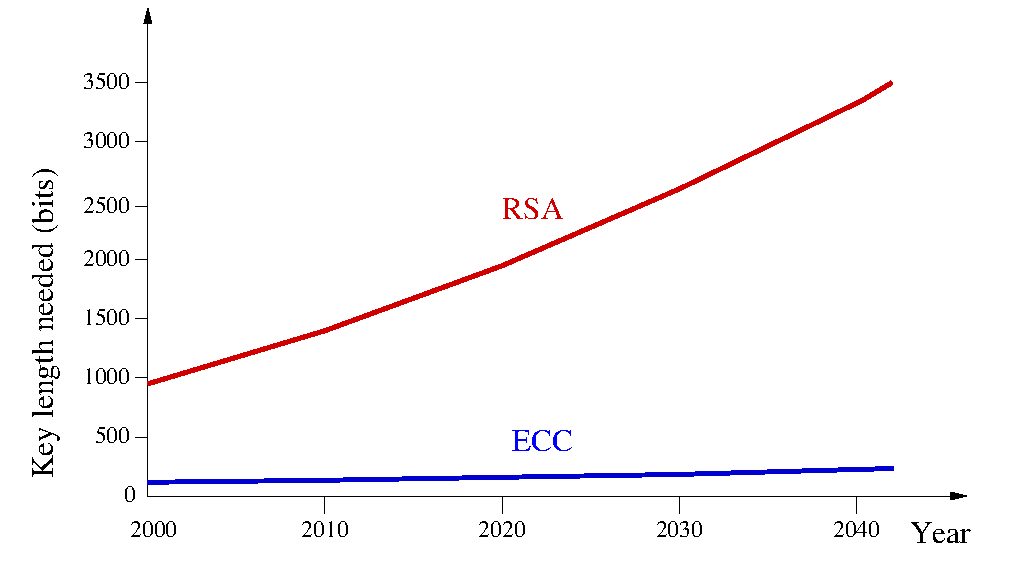
\includegraphics[scale=0.7]{figures/RSAKeyLength-2}
\caption{Prognosis of the key lengths to be regarded safe for RSA and
  Elliptic Curves\vspace{1ex}} 
\label{RSAKeylength}
\end{center}
\end{figure}

In addition, a digital signature can be processed 10-times faster with ECC
than with RSA.  However, verification of a given signature is still more
efficient with RSA than with ECC. Refer to
figure~\ref{ThousandBitMultiplications} (source: Dr.~J.\ Merkle, Elliptic
Curve Cryptography Workshop, 2001) for a comparison.  The reason is that
RSA public keys can be chosen relatively small as long as the secret key is
long enough.

% -> Figure 2
\begin{figure}[ht]
\begin{center}
\vspace{1.5cm}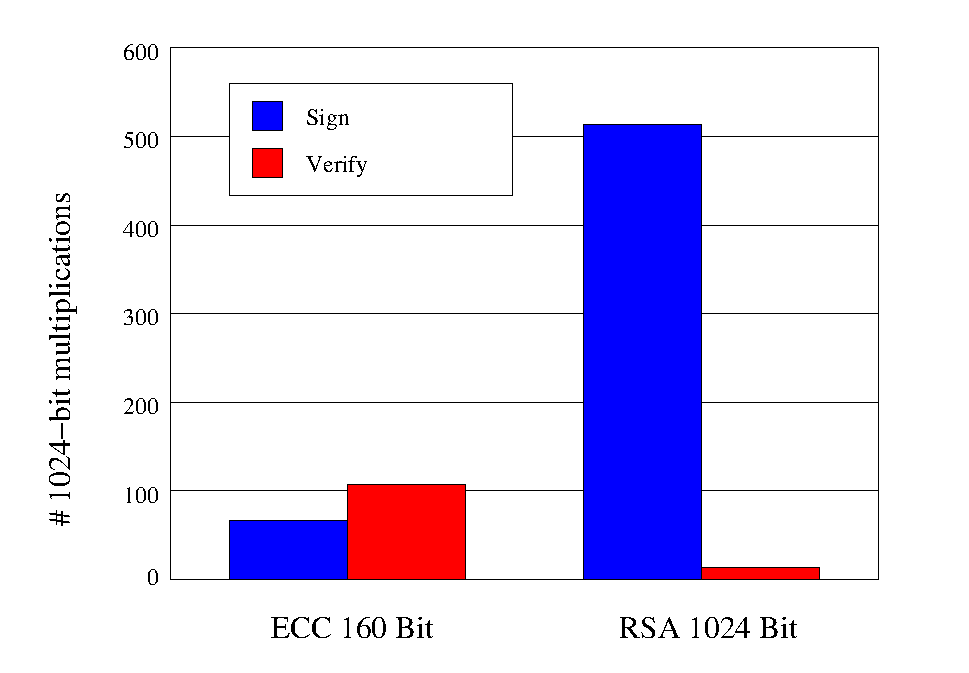
\includegraphics[scale=0.7]{figures/ECCRSA}
\caption{Comparison of signing and verification time for RSA and Elliptic Curves} 
\label{ThousandBitMultiplications}
\end{center}
\end{figure}

Nevertheless, thin clients like smart cards usually have to store the (long)
secret key and have to process a digital signature rather than verify one.
Therefore, there is a clear advantage in using ECC in terms of efficiency.
\par
\smallskip
Nowadays, the major problem with ECC implementations is the lack of standardization.
There is only one way to implement RSA, but there are many ways for ECC: One can work with
different sets of numbers, different (elliptic) curves --- described by parameters\footnote{%
see chapter \ref{ECC-Crypto}
} --- ,
and a variety of representations of the elements on the curve. Each choice has its
advantages and disadvantages, and one can certainly construct the most efficient for
each application. However, this causes problems in interoperability. But if all
ECC-tools should be able to communicate with each other, they will have to support
all different algorithms, which might put the advantage of efficient computation and
the need of less storage capacity to the contrary.

\begin{sloppypar}
Therefore, international standardization organizations like IEEE (P1363),
ASC (ANSI X9.62, X9.63), ISO/IEC as well as major players like RSA labs or
Certicom have recently started standardization initiatives. While the IEEE
only describes the different implementations, the ASC has explicitly stated
10 elliptic curves and recommends their usage. The advantage of the ASC
approach is that one needs only a single byte to indicate which curve is
meant. However, it is not yet clear whether the ASC curves will become a de
facto standard.
\end{sloppypar}

Although we see no need to replace RSA in any application today\footnote{%
Current information about the security of the RSA algorithm can be found in 
chapter \ref{SecurityRSA}.}, one should
take the usage of ECC-based tools into consideration whenever a new system
is set up --- in particular, when the tool should be available beyond 2005\footnote{%
Compare the recommendation of GISA: ``Fitting Crypto Algorithms'' from October 24th, 2002.
}.


\section{Elliptic curves -- history}

Mathematicians have been researching elliptic curves for over 100 years.
Over the course of time, many lengthy and mathematically complex results
have been found and published which are connected to elliptic curves. 
A mathematician would say that elliptic curves (or the mathematics behind
them) are widely understood. This research was originally purely 
mathematical. That is to say, elliptic curves were investigated, for 
example, in the mathematical areas of number theory and algebraic 
geometry, which are generally highly abstract. Even in the recent
past, elliptic curves played an important role in pure mathematics.
In 1993 and 1994, Andrew Wiles\index{Wiles, Andrew} published 
mathematical works that triggered enthusiasm far beyond the specialist
audience. In these works, he proved a conjecture put forward in the 1960's.
To put it short, this conjecture was concerned with the connection 
between elliptic curves and what are called module forms. What is
particularly interesting for most people is that the works of Wiles
also proved the famous second theorem of Fermat. Mathematicians had
spent centuries (Fermat lived from 1601 to 1665) trying to find a
strict proof of this theorem. Understandably, therefore, Wiles' proof
got a good response. Fermat formulated his theorem as follows 
(written in the border of a book):

\begin{quote} {\em
Cubum autem in duos cubos, aut quadratoquadratum in duos quadratoquadratos, et
generaliter nullam in infinitum ultra quadratum potestatem in duos ejusdem
nominis fas est dividere: cujus rei demonstrationem mirabilem sane detexi. Hanc
marginis exiguitas non caperet.
} \end{quote}

With a free translation, using the denotation of modern mathematics, this means: \\
No positive whole numbers $x, y$ and $z$ greater than zero exist such that $x^n +y^n = z^n$ for $n>2$. I have found an amazing proof of this fact, but there is
too little space within the confines of this book to include it.

This is truly amazing: A statement that is relatively simple to understand (we
are referring to Fermat's second theorem here) could only be proved after such a
long period of time, although Fermat himself claimed to have found a proof.
What's more, the proof found by Wiles is extremely extensive (all of Wiles
publications connected with the proof made up a book in themselves). This should
therefore make it obvious that elliptic curves are generally based on highly
complex mathematics.

Anyway that's enough about the role of elliptic curves in pure mathematics. 
In 1985 Neal Koblitz\index{Koblitz, Neal} and Victor Miller\index{Miller, Victor}
independently suggested using elliptic curves in cryptography. Elliptic 
curves have thus also found a concrete practical application. 
Another interesting area of application for elliptic curves is for
factorizing whole numbers \index{Factorization} (the RSA cryptographic system
is based on the \index{Complexity} difficulty/complexity of finding prime
factors of an extremely large number;  compare section \ref{SecurityRSA}.).
In this area, procedures based on elliptic curves have been investigated and
used since 1987 (compare section \ref{ECC-Factorization}). \\
There are also prime number tests\index{Prime number!test} based on elliptic
curves.
% (s. Anmerkung U. Kuehn)

Elliptic curves are used differently in the various areas. Encryption
procedures based on elliptic curves are based on the difficulty of a problem
known as elliptic curve discrete logarithm\index{Logarithm problem!discrete}.
The factorization of whole numbers uses the fact that a large number of
elliptic curves can be generated for a natural composite number $n$ with
several prime factors; however, these curves are not then groups for composite
$n$. More information about this can be found under the chapter \ref{ECC-Factorization}.

\section{Elliptic curves -- mathematical basics}

This section provides information about \index{Group} {\em groups} and
\index{Field} {\em fields}.

\subsection{Groups}

Because the term {\em group} is used differently in everyday language than in
mathematics, we will, for reasons of completeness, begin by introducing the
essential statement of the formal definition of a group:
\begin{itemize}
   \item A group is a non-empty set $G$ on which an operation ``$\cdot$''. The set $G$ is closed under this operation, which means that for any two elements $a, b$ taken from $G$, performing the operation on them gives an element in $G$, i.e. $ab=a\cdot b$ lies in $G$.
   \item For all elements $a, b$ and $c$ in $G$: $(ab)c = a(bc)$ (associative law).
   \item There exists an element $e$ in $G$ that behaves neutrally with respect
to the operation $\cdot$. That means that for all a in the set $G: ~ae = ea = a$.
   \item For each element $a$ in $G$ there exists a so-called inverse\footnote{The inverse is uniquely determined because if $x,y\in G$ are each inverse to $a$, i.e. $ax=xa=e$ and $ay=ya=e$, then $x=xe=x(ay)=(xa)y=ey=y$.} element $a^{-1}$ in $G$ such that: $aa^{-1} = a^{-1}a = e$.
\end{itemize}
If also $ab = ba$ (commutative law) for all $a, b$ in $G$, then we call the group an {\em Abelian} group.

Since we may define different operations on the same set, we distinguish them by giving them different names (e.g.\ $+$ addition or $\cdot$ multiplication).

The simplest example of an (Abelian) group is the group of whole numbers under
the standard operation of addition. The set of whole numbers is denoted as
${\mathbb Z}$. ${\mathbb Z}$ has an infinite number of elements, because
${\mathbb Z} = \{ \cdots, -4, -3, -2, -1, 0, 1, 2, 3, 4, \cdots\}$. For example, the
operation of $1+2$ lies in ${\mathbb Z}$, for $1+2 = 3$ and $3$ lies in
${\mathbb Z}$. The neutral element in the group ${\mathbb Z}$ is $0$. The
inverse element of $3$ is $-3$, for $3+(-3) = 0$.

For our purpose, so-called {\em finite} groups play an important role. This means that these exists a set
$\mathcal{M}$ with a fixed number of elements and an operation $+$ such that the
above conditions are fulfilled. One example of this is any set ${\mathbb Z}_n$
where ${\mathbb Z}_n = \{0, 1, 2, 3, \cdots, n-1\}, n$ is a positive whole number
and the operation is addition mod $n$, i.e. $a$ and $b$ in ${\mathbb Z}_n$ are
subject to the operation $a+b \;{\rm mod~} n$.

\paragraph{Cyclic groups}\index{Group!cyclic}
Cyclic groups\footnote{Cyclic groups can be in general also endless like the additive group of the integer numbers. We consider here only finite cyclic groups.} are those groups $G'$ that possess an element $g$
from which the group operation can be used to generate all other
elements in the group. This means that for each element $a$ in
$G'$ there exists a positive whole number $i$ such that if $g$ is
subject to the operation $i$ times (i.e. ``$g\cdot i$''),
$g+g+\cdots+g = a$ (additive group) or $g^i = g\cdot g \cdots g = a$
(multiplicative group). The element $g$ is the {\em generator} of
the cyclic group --- each element in $G'$ can be generated using
$g$ and the operation.

\paragraph{Group order}
Now to the order of an element of the group: Let $a$ be in $G$. The smallest
positive whole number $r$ for which $a$ subject to the operation with itself $r$
times is the neutral element of the group $G'$ (i.e.: $r \cdot a = a+a+\cdots+a =
e$ respectively $a^r = e$), is called the {\em order} of $a$.

The order of the group is the number of elements in the set $G$.

\subsection{Fields}

In mathematics, one is often interested in sets on which at least two (group) operations are defined --- frequently called addition and multiplication. Most prominent are so called fields.

A field is understood to be a set $K$ with two operations
(denoted as $+$ and $\cdot$) which fulfils the following conditions:
\begin{itemize}
   \item The set $K$ forms an Abelian group together with the operation $+$
(addition), where $0$ is the neutral element of the operation $+$.
   \item The set $K\setminus\{ 0\}$ also forms an Abelian group
together with the operation $\cdot$ (multiplication).
   \item For all elements $a, b$ and $c$ in $K$, we have $c\cdot (a+b) = c \cdot a + c
\cdot b$ and $(a+b) \cdot c = a \cdot c + b \cdot c$ (distributive law).
\end{itemize}

Fields may contain an infinite number of elements (e.g.\ the field of real numbers). They are called {\em infinite} fields. In contrast we call a field
{\em finite}, if it contains only a finite number of elements (e.g.\ ${\mathbb Z}_p = \{0, 1, 2, 3, \cdots, p-1\}$
, where $p$ is a prime. ${\mathbb Z}_p$ with addition mod $p$ and multiplication
mod $p$).
\index{Field!characteristic}
\paragraph{Characteristic of a field}
Let $K$ be a field and $1$ be the neutral element of $K$ with
respect to the multiplicative operation ``$\cdot$''. Then the characteristic of $K$ is said to be the order of $1$ with respect to the additive operation. This means that the characteristic of $K$ is the smallest positive integer $n$ such that
$$ \underbrace{1+1+\dots+1}_{\hbox{$n$ times}} =0 .
$$
If there is no such $n$, i.e. if $1+1+\dots+1\ne 0$ no matter how many $1$s we add, then we call $K$ a field
with characteristic $0$.

Thus, fields with characteristic $0$ are infinite since they contain the (pairwise distinct) elements $1$, $1+1$, $1+1+1$, \dots. On the other hand, fields with finite characteristic may by finite or infinite.

If the characteristic is finite, it has to be prime. This fact can easily be proved: Assume $n=pq$, $p,q<n$, is the characteristic of a field $K$. By definition of $n$, the elements $\bar p=\underbrace{1+1+\dots+1}_{\hbox{$p$ times}}$, $\bar q=\underbrace{1+1+\dots+1}_{\hbox{$q$ times}}$ of $K$ are not equal to $0$. Thus, there exist inverse elements $\bar p^{-1},\bar q^{-1}$ with respect to multiplication. It follows that $(\bar p\bar q)(\bar p^{-1}\bar q^{-1})=1$, which contradicts the fact that $\bar p\bar q=\bar n=\underbrace{1+1+\dots+1}_{\hbox{$n$ times}}=0$ and, hence, $\underbrace{(\bar p\bar q)}_{=0}(\bar p^{-1}\bar q^{-1})=0$.

\begin{remark}{:}\\
The field of real numbers has the characteristic $0$; the field ${\mathbb Z}_p$ has
the characteristic $p$. If $p$ is not prime, ${\mathbb Z}_p$ is not a field at all.
\end{remark}

The most simple field is ${\mathbb Z}_2=\{ 0,1\}$. It contains only two elements, the neutral elements with respect to addition and multiplication. In particular, we have $0+0=0$, $0+1=1+0=1$, $1+1=0$, $1\cdot 1=1$, $0\cdot 0=0\cdot 1=1\cdot 0=0$.

\index{Field!finite}
\paragraph{Finite Fields}
As mentioned above, each finite field has a characteristic $p\ne 0$, where $p$ is a prime. On the other hand, given a prime $p$ there is a field which has exactly $p$ elements, that is ${\mathbb Z}_p$.

However, the number of elements of a field need not be prime in general. For example, it is not hard to construct a field with $4$ elements\footnote{%
The set $K=\{0,1,a,b\}$ fitted with the operation defined in the tabular below is a field:\\
$
\begin{array}{|c||c|c|c|c|} 
\hline 
+ & 0 & 1 & a & b \\
\hline \hline
0 & 0 & 1 & a & b \\
\hline 
1 & 1 & 0 & b & a \\
\hline 
a & a & b & 0 & 1 \\
\hline 
b & b & a & 1 & 0 \\
\hline 
\end{array} \qquad {\rm ~und~} \qquad
\begin{array}{|c||c|c|c|c|} 
\hline 
\cdot & 0 & 1 & a & b  \\
\hline \hline
0 & 0 & 0 & 0 & 0 \\ 
\hline 
1 & 0 & 1 & a & b \\ 
\hline 
a & 0 & a & b & 1 \\ 
\hline 
b & 0 & b & 1 & a \\
\hline 
\end{array} 
$  \\
}.

One can show that the order of any field is a prime power (i.e. the power of a prime number). On the other hand, we can construct a field with $p^n$ elements for any given prime $p$ and positive integer $n$. Since two fields that have the same number of elements can not be distinguished\footnote{If $K,K'$ are fields with $k=p^n$ elements, then there is a one-to-one map $\varphi:K\to K'$, that respects the arithmetic of the field. Such a map is called an isomorphy. Isomorphic fields mathematically behave in the same way so that   it makes no sense to distinguish between them. For example, ${\mathbb Z}_2$ und $K'=\{ ZERO,ONE\}$ with zero-element $ZERO$ and one-element $ONE$ are isomorphic. We note that mathematical objects are only defined by their mathematical properties.}, we say that there is {\bf the field with $p^n$ elements} and denote it by $GF(p^n)$. Here $GF$ stands for {\it Galois Field} to commemorate the French Mathematician Galois.

The fields $GF(p)$ of prime order play a prominent role. They are called prime fields and often denoted by ${\mathbb Z}_p$\footnote{For prime fields additive as well as multiplicative group are cyclic. Furthermore, each field $GF(p^n)$ contains a subfield that is isomorphic to the prime field ${\mathbb Z}_p$.}.



% -----------------------------------------------------------------------------
\section{Elliptic curves in cryptography}\label{ECC-Crypto}

In cryptography elliptic curve are a useful tool. Such curves are described by some equation. A detailed analysis has shown that curves of the form\footnote{This curve is given by the zeros of a {\it polynomial}\index{Polynomial} $F$ of degree three in three variables. In general, expressions of the form
$P=\sum_{i_1,\dots,i_n\in\N_0} a_{i_1\dots i_n} x_1^{i_1}\dots x_n^{i_n}$ with coefficients $a_{i_1\dots i_n}\in K$ are called polynomials in $n$ variables $x_1,\dots,x_n$ with underlying field $K$, if ${\rm deg\,} P:=\max\{i_1+\dots +i_n: a_{i_1\dots i_n}\ne 0\}$ is finite, i.e. the sum has only finitely many non-zero terms (monomials). The sum of the exponents of the variables of each term of the sum is at most $3$, at least one term of the sum has a single variable with $3$ as value of the according exponent.}
\begin{equation}
 F(x_1,x_2,x_3)=-x_1^3+x_2^2x_3+a_1x_1x_2x_3-a_2x_1^2x_3+a_3x_2x_3^2-a_4x_1x_3^2-a_6x_3^3=0,
\label{eccbasisgleichung}
\end{equation}
are especially useful. The variables $x_1,x_2,x_3$ and parameters $a_1,\dots,a_4,a_6$ are elements of a given field $K$, which has certain properties that are make it useful from the cryptographic point of view. The underlying field $K$ might be the well known field of real numbers or some finite field (see last section).
In order to obtain a cure that is useful for cryptography, the parameters have to be chosen in a way that the following conditions hold
$$ \frac{\partial F}{\partial x_1}\ne 0, \quad \frac{\partial F}{\partial x_2}\ne 0, \quad
\frac{\partial F}{\partial x_3}\ne 0 .
$$
We identify points on the curve that can be derived from each over by multiplying each component with some scalar. This makes sense since $(x_1,x_2,x_3)$ solves (\ref{eccbasisgleichung}) if and only if $\alpha (x_1,x_2,x_3)$ ($\alpha\ne 0$) does. Formally, this means that we consider classes of equivalent points instead of single points, where points are called equivalent if one is the scalar multiple of the other one.
\\ If we put $x_3=0$ in the basic equation (\ref{eccbasisgleichung}), then this equation collapses to $-x_1^3=0$, leading to $x_1=0$. Thus, the equivalence class which includes the element $(0,1,0)$ is the only one that contains a point with $x_3=0$. For all points on the curve that are not equivalent to $(0,1,0)$, we may apply the following transformation
$$ K\times K\times (K\setminus\{0\})\ni (x_1,x_2,x_3) \mapsto (x,y):=\left( \frac{x_1}{x_3}, \frac{x_2}{x_3}\right) \in K\times K \, ,
$$
which reduces the number of variables to two instead of three. We note that the
basic equation (\ref{eccbasisgleichung}) $F(x_1,x_2,x_3)=0$  was chosen in a
way that this transformation leads to the famous so-called
Weierstrass-Equation\footnote{Karl Weierstrass\index{Weierstrass, Karl}, 31.10.1815$-$19.12.1897, German
mathematician, famous for his rigorous formal approach to mathematics.} holds
\begin{equation}
 y^2+a_1xy+a_3y = x^3+a_2x^2+a_4x+a_6 \, .
\label{ell}
\end{equation}
Since all but one point (i.e. equivalence class) of the elliptic curve can be described using equation (\ref{ell}), this equation is often called the elliptic equation, and its solutions written as
$$ {\bf E} = \left\{(x,y)\in K\times K \, |\, y^2+a_1xy+a_3y = x^3+a_2x^2+a_4x+a_6  \right\} \cup \{{\cal O} \}.
$$
Here, ${\cal O}$ represents the point $(0,1,0)$ that is loosely speaking mapped to infinity by the transformation (division by $x_3$) that reduces the three variables to two.

\begin{figure}[ht]
\begin{center}
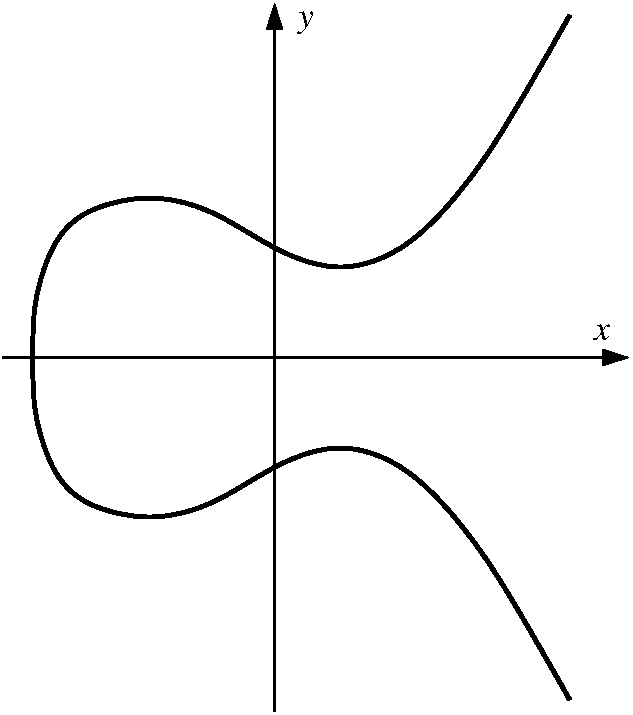
\includegraphics[scale=0.60]{figures/elliptic-curve}
\caption{Example of an elliptic curve with the real numbers as underlying field.\vspace{1ex}} 
\label{ExampleEllipticCurve}
\end{center}
\vskip -10 pt
\end{figure}

In contrast to figure \ref{ExampleEllipticCurve} only finite fields $K=GF(p^n)$ are used in elliptic curve cryptography. The reason is loosely speaking that in modern communication engineering data processing is always based on discrete data (simply because computers accept only discrete data).

For practical reasons, it turned out to be useful to take either $GF(p)$ with a large prime $p$ or $GF(2^n)$ with a (large) positive integer $n$. Using $GF(p)$ has the advantage of providing a relatively simple arithmetic; on the other hand $GF(2^n)$ allows a binary representation of each element that supports the way computers work. Other fields like, for example, $GF(7^n)$ do not have any of these advantages and are, thus, not considered, although there is no mathematical reason why they should not.

A coordinate transformation can result in a simpler version\footnote{Such a coordinate transformation is combination of a rotation and a dilatation of the coordinate system without changing the elliptic curve itself.} of the Weierstrass equation\index{Weierstrass, Karl}. Depending whether $p>3$, different transformations are used, and we obtain
\begin{itemize}
\item in case of $GF(p)$, $p>3$, the elliptic curve equation of the form
\begin{equation}
 y^2 = x^3 + ax + b
\label{ellp}
\end{equation}
with $4a^3+27b^2\ne 0$
\item in case of $GF(2^n)$ the elliptic curve equation of the form 
\begin{equation}
 y^2+xy = x^3 + ax^2 + b
\label{ell2}
\end{equation}
with $b\ne 0$\footnote{The form (\ref{ellp}) is called the standard form of the Weierstrass-equation\index{Weierstrass, Karl}. If the characteristic of the field is $2$ or $3$, we obtain $4=0$ respectively $27=0$, which means that the condition on parameters $a,b$ collapse. Loosely speaking, this is the reason why the transformation to the standard form does not work in these cases.}.
\end{itemize}
This conditions on the parameters $a,b$ ensure that the elliptic equation can be used in the context of cryptography\footnote{Formally we call such curves non singular.}.

Let $|E|$ denote the number of elements of an elliptic curve $E$ given an underlying field $GF(k)$ (for practical reasons either $k=p$ with $p$ prim or $k=2^n$). Then Hasse's theorem\cite{ec:Silverman1986} yields $| \, |E| - k-1\,| \le 2\cdot \sqrt{k}$. This Inequality is equivalent to $k+1 - 2\sqrt{k} < |E| < k+1+2\sqrt{k}$. In particular, this means that the number of elements of an elliptic curve is approximately $k$ (for large $k$). 

% -----------------------------------------------------------------------------
\section{Operating on the elliptic curve}

In order to work with elliptic curves in practice, we define an operation (often written in an additive way $+$) on the set of points on the curve. If we have a curve over the field $GF(p)$, we define the commutative operation $+$ by
\begin{enumerate}
\item $P+{\cal O}={\cal O}+P=P$ for all $P\in E$,
\item for $P=(x,y)$ and $Q=(x,-y)$ we set $P+Q={\cal O}$,
\item for $P_1=(x_1,x_2),P_2=(x_2,y_2)\in E$ with $P_1,P_2\ne {\cal O}$ and $(x_2,y_2)\ne (x_1,-y_1)$ we set $P_3:=P_1+P_2$, $P_3=(x_3,y_3)$ defined by
$$ x_3:=-x_1-x_2+\lambda^2 \, , \qquad y_3:=-y_1+\lambda (x_1-x_3)
$$
with the auxiliary quotient
$$ \lambda:=\left\{ \begin{array}{cl} \frac{y_1-y_2}{x_1-x_2} & {\rm if~} P_1\ne P_2, \\
                                     \frac{3x_1^2+a}{2y_1} & {\rm if~} P_1=P_2. \end{array} \right.
$$
\end{enumerate}
In particular, we obtain $-P=(x,-y)$ for $P=(x,y)\in E$.

If we deal with a curve over the field $GF(2^n)$, we define the operation $+$ in an analogous way by
\begin{enumerate}
\item $P+{\cal O}={\cal O}+P=P$ for all $P\in E$,
\item for $P=(x,y)$ and $Q=(x,x+y)$ we set $P+Q={\cal O}$,
\item for $P_1=(x_1,x_2),P_2=(x_2,y_2)\in E$ with $P_1,P_2\ne {\cal O}$ and $(x_2,y_2)\ne (x_1,x_1+y_1)$ we set $P_3:=P_1+P_2$, $P_3=(x_3,y_3)$ defined by
$$ x_3:=-x_1+x_2+\lambda+\lambda^2+a \, , \qquad y_3:=y_1+x_3+\lambda (x_1+x_3)
$$
with auxiliary quotient
$$ \lambda:=\left\{ \begin{array}{cl} \frac{y_1+y_2}{x_1+x_2} & {\rm if~} P_1\ne P_2, \\
                                   x_1+\frac{y_1}{x_1} & {\rm if~} P_1=P_2. \end{array}\right.
$$
\end{enumerate}
In particular, we obtain $-P=(x,-y)$ for $P=(x,y)\in E$.

(Note that $-(-P)=(x,x+(x+y))=(x,2x+y)=(x,y)$, since the underlying field
has characteristic $2$.)\footnote{An animation of the addition of points
on elliptic curves can be found on the Certicom\index{Certicom} homepage \\
\url{http://www.certicom.com/resources/ecc_tutorial/ecc_tutorial.html}}

One can verify that $+$ defines a group operation on the set $E\cap\{\cal O\}$.
In particular this means that the sum of two points is again a point on the
elliptic curve. How his operation works is geometrically visualized in the
following section.

% \newpage
\begin{figure}[htbp]
\subsection*{How to add points on an elliptic curve}
The following figures show how points on an elliptic curve over the field of real numbers are summed up using affine coordinates.
We note that the point infinity ${\cal O}$ cannot be shown in the affine plane.  
\begin{center}
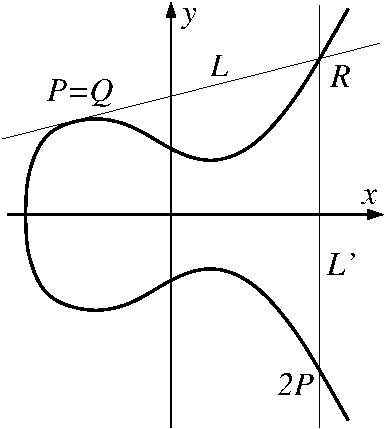
\includegraphics[scale=1.08]{figures/ec-mult2}
\caption{Doubling of a point} 
\vspace{\floatsep}
\vskip +20 pt
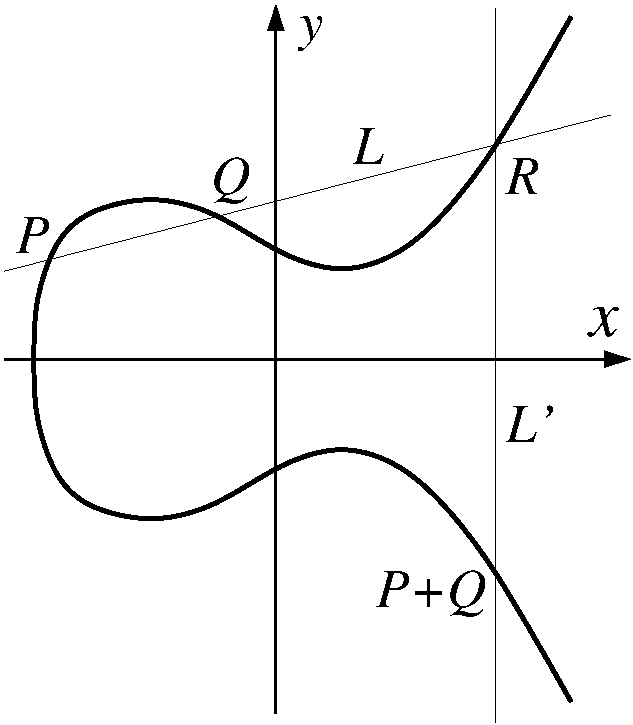
\includegraphics[scale=0.65]{figures/ec-add}
\caption{Summing up two different points over the real number field} % \footnotemark }
\end{center}
\end{figure}
\enlargethispage{+20pt}
\newpage


% -----------------------------------------------------------------------------
\section{Security of elliptic-curve-cryptography: The ECDLP}

As mentioned above in section \ref{ECC-Crypto}, we only consider elliptic curves over the finite\footnote{Discrete in contrast to continuous.} fields $GF(2^n)$ or $GF(p)$ (for a large prime $p$). This means that all parameters that describe the curve are taken from this underlying field. If $E$ is an elliptic curve over such a field and $P$ is a point on the curve $E$, then we can derive for all positive integers $m$
$$ mP := \underbrace{P+P+\dots+P}_{\hbox{$m$ times}} \, .
$$
Looking on this operation from the cryptographic point of view, it turns out to be very interesting by the following reason: On the one hand one needs only $\log m$ operations to calculate $mP$ --- one simply has to calculate $P$, $2P$, $2^2P$, $2^3P$, \dots, write $m$ in a binary form and finally add all these multiples $2^kP$ of $P$ with respect to the binary representation of $m$ --- on the other hand it seems to be very hard to find $m$ given $P$ and $Q=mP$ on $E$. Of course, we may simply calculate $P,2P,3P,4P,5P,\dots$ and compare each of them with $Q$. But this will take as much as $m$ operations.

Yet there is no algorithm known that efficiently derives $m$ given $P$ and $G$. The best algorithms known so far need about $\sqrt{q}$ operations where $q$ is the (largest) prime factor of $p-1$, in case the underlying field is $GF(p)$; here $m$ should be between $1$ and $q$ liegen so that one needs at most $\log q$ operations to calculate $mP$. However, the quotient $\frac{\sqrt{q}}{\log q}$ tends to $+\infty$ very fast for large $q$.

If we choose the parameters sufficiently large (for example, let $p$ be prime and at least $160$ bits long), an computer will easily be able to calculate $mP$ (in less than a second). The {\it inverse problem} however, to derive $m$ from $mP$ and $P$, can (still) not be solved in reasonable time.

This problem is known as the ``Elliptic Curve Discrete Logarithm Problem'' (for short ECDLP\index{ECDLP}).

\vskip +5 pt

In elliptic curve cryptography we formally look at points on the elliptic curve as elements of a group with point addition $+$ as operation. Furthermore, we use only elliptic curves that have a sufficiently large number of points. However, in special cases curves may be weak and not useful due to other reasons. For such special cases the ECDLP can be much easier to solve than in the general case. This means that one has to look carefully at the parameters when choosing an elliptic curve for cryptographic applications.

Not useful for cryptography are {\em a-normal} (that are curves over ${\mathbb Z}_p$,
for which the set ${\bf E}$ consists of exactly $p$ elements) and {\em supersingular} curves (that are curves, for which the ECDLP can be reduced to the ``normal'' discrete logarithms in another, smaller finite field). This means that there are cryptographically useful and non-useful elliptic curves. Given the parameters $a$ and $b$, it is possible to determine whether a curve is useful or not. In many publications one can find parameters that turned out to be useful for cryptography. The open (scientific) discussion guarantees that these results take into account latest research.
\vskip +5 pt

Given a secure curve, the time that is needed to solve the ECDLP is strongly correlated with parameter $p$ in case $GF(p)$ respectively $n$ in case of $GF(2^n)$. The larger these parameters become, the more time an attacker needs to solve the ECDLP --- at least with the best algorithms known so far. Experts recommend bit-lengths of $200$ for $p$ for secure curves. A comparison with RSA modulus length shows why elliptic curves are so interesting for applications. We note that the computation effort for signing and encryption is closely related to the bit-length of the parameters. In addition the initiation process, i.e. the generation of the private-public-key-pair, becomes more complicated the larger $p$ is. Thus, one looks for the smallest parameters that still come along with the security required. It is remarkable that a length of $200$ bits for $p$ is sufficient to construct a {\em good} elliptic curve that is as secure as RSA with a $1024$ bit \index{RSA!modulus} RSA modulus (as far as we know today). For short, the reason for this advantage of ECC lies in the fact that the best algorithms known for solving the ECDLP need exponential time while the best algorithms for factorizing are sub-exponential (number field sieve, quadratic sieve or factorizing with elliptic curves). Hence, the parameters for a cryptosystem that is based on the problem of {\em factorizing large integers} have to be larger than the parameters for a system based on ECDLP.


% -----------------------------------------------------------------------------
\section{Encryption and signing with elliptic curves}

\begin{sloppypar}
  The {\em elliptic curve discrete logarithm
    problem}\index{Problem of discrete logarithm} (ECDLP) \index{ECDLP} is the basis for elliptic curve cryptography. Based on this problem, there are different signature schemes. In order to apply one of these, we need:
\end{sloppypar}
\begin{itemize}
    \item An elliptic curve {\bf E} with an underlying field $GF(p^n)$.
    \item A prime $q\ne p$ and a point $G$ on the elliptic curve ${\bf E}$ with order $q$. This means that $qG={\cal O}$ and $rG\ne {\cal O}$ for all $r\in \{1,2,\dots,q-1\}$. Thus $q$ is a factor of the group order (i.e. the number of elements) $\#{\bf E}$ of $E$. Since $q$ is prime, $G$ generates a cyclic sub-group of ${\bf E}$ of order $q$.
\end{itemize}
The parameters mentioned are often called \index{Domain parameter}
{\em Domain} parameter. They describe the elliptic curve ${\bf E}$ and 
the cyclic sub-group of ${\bf E}$ on which the signature scheme is based.

\par
%\smallskip
%{\bf Encryption:}
\subsection{Encryption}

Using elliptic curves one can construct a key exchange protocol based on the Diffie-Hellman protocol \index{Diffie-Hellman} (see chapter \ref{DH-KeyExch}). The key exchanged can be used for a subsequent symmetric encryption. We note that in contrast to RSA there is no pair of private and public key that can be used for encryption and decryption!

In the notation of elliptic curves, the Diffie-Hellman protocol reads as follows: First both partners (A und B) agree on a group $G$ and an integer $q$. Then they choose $r_A,r_B\in\{1,2,\dots,q-1\}$ at random, derive the points $R_A=r_AG$, $R_B=r_BG$ on the elliptic curve and exchange them (using an insecure channel). After that A easily obtains $R=r_AR_B$; B gets the same point ($R=r_Ar_B G$) by calculating $r_BR_A=r_Br_AG=r_Ar_BG=R$. We note that $R_A,R_B$ are easy to derive as long as $r_A$ respectively $r_B$ are known $G$. However, the inverse operation, to get $R_A$ respectively $R_B$ from $r_A$ respectively $r_B$ is hard.
\\ Using the best algorithms known so far, it is impossible for any attacker to obtain $R$ without knowing either $r_A$ or $r_B$ --- otherwise he would have to solve the ECDLP.

In order to prohibit a ``Man-in-the-middle"{}~attack, one may sign the values $G,q,R_A,R_B$ as described in chapter \ref{Impersonalisierungsattacke}.


\par
%\smallskip 
%{\bf Signing:}
\subsection{Signing}

Using the \index{DSA} DSA signature scheme, one can proceed as follows: The signing party chooses a (non-trivial) number $s\in{\mathbb Z}_q$, which will be the private key, and publishes $q$, $G$ and $R=sG$. We note that $s$ cannot be obtained from $G$ and $R$ are not sufficient --- a fact on which the security of the signature scheme is based.

Given the message $m$, which should be signed, one first constructs a digital finger print using a hash-algorithm $h$ such that $h(m)$ has its values in $\{0,1,2,\dots, q-1\}$. Thus, $h(m)$ can be considered as an Element of ${\mathbb Z}_q$. Then the signing party chooses a random number $r\in{\mathbb Z}_q$ and derives $R=(r_1,r_2)=rG$. We note that the first component $r_1$ of $R$ is an element of $GF(p^n)$. This component will then be projected onto ${\mathbb Z}_q$, i.e. in case of $n=1$ it is interpreted as the remainder of an element of $\{0,1,\dots,p-1\}$ divided by $q$. This projection of $r_1$ onto ${\mathbb Z}_q$ is denoted by $\bar r_1$. Then one determines $x\in {\mathbb Z}_q$ such that
$$ rx-s\bar r_1-h(m)=0 .
$$
The triple $(m,r_1,x)$ is then published as the digital signature of message $m$.

\par
%\smallskip 
%{\bf Signature Verification:}
\subsection{Signature verification}

In order to verify a signature, one has to build $u_1=h(m)/x$, $u_2=\bar r_1/x$ (in ${\mathbb Z}_q$ and derive
$$ V=u_1G+u_2Q .
$$
Since we have $Q=sG$, the point $V=(v_1,v_2)$ satisfies $v_1=u_1+u_2s$. We note that this operations take place in the field $GF(p^n)$. The projection of $GF(p^n)$ on ${\mathbb Z}_q$ mentioned above should be chosen in such a way that $\bar v_1=u_1+u_2s$ is an element of ${\mathbb Z}_q$. Then it follows that
$$ \bar v_1=u_1+u_2s=h(m)/x+\bar r_1 s/x=(h(m)+\bar r_1s)/x=rx/x=r .
$$
Since $R=rG$, we obtain $\bar v_1=\bar r_1$, i.e. $R$ and $V$ coincide modulo the projection onto ${\mathbb Z}_q$.


% -----------------------------------------------------------------------------
\hypertarget{faktell}{}
\section{Factorization using elliptic curves} \label{ECC-Factorization}

There are factorization%
\footnote{Especially John M. Pollard \index{Pollard, John M.} was involved
in the development of many different factorization algorithms; also at
factorization with ECC he was one of the leading heads. As an employee
of British Telekom he never published much. At the RSA data Security Conference
in 1999 he was awarded for his ``outstanding contributions in mathematics'':
\href{http://www.eff.org/Privacy/Crypto_misc/DESCracker/HTML/19990118_rsa_awards.html}
{\texttt{http://www.eff.org/Privacy/Crypto\_misc/DESCracker/HTML/19990118\_rsa\_awards.html}}.
}
algorithms based on elliptic curves%
\footnote{In 1987 H.W. Lenstra published
a factorization algorithm, based on elliptic curves (see \cite{ec:Lenstra1987}).
The biggest compound number currently 
factorized\index{Factorization!factoring records} with elliptic curves is 
the number $ 628^{59}-1, $ which has 55 decimal digits. It was
found Oct. 6th, 2001 by M. Izumi 
(See \hyperlink{Lenstra2}{ECMNET}\index{ECMNET}).
}. 
More precisely, these procedures exploit the fact that elliptic curves can
be defined over ${\mathbb Z}_n$ ($n$ composite number). Elliptic curves 
over ${\mathbb Z}_n$ do not form a group, because not every point on such 
an elliptic curve has an inverse point. This is connected with the fact 
that - if $n$ is a composite
number - there exist elements in ${\mathbb Z}_n$ that do not have an inverse
with respect to multiplication mod $n$. In order to add two points on an
elliptic curve over ${\mathbb Z}_n$, we can calculate in the same way as on
elliptic curves over ${\mathbb Z}_p$. Addition of two points (on an elliptic
curve over ${\mathbb Z}_n$), however, fails if and only if a factor of $n$ has
been found. The reason for this is that the procedure for adding points on
elliptic curves gives elements in ${\mathbb Z}_n$ and calculates the inverse
elements for these (with respect to multiplication mod $n$) in ${\mathbb Z}_n$.
The extended \index{Euclidean algorithm} Euclidean algorithm is used here. If
the addition of two points (that lie of an elliptic curve over ${\mathbb Z}_n$)
gives an element in ${\mathbb Z}_n$ that does not have an inverse element in
${\mathbb Z}_n$, then the extended Euclidean algorithm delivers a genuine factor
of $n$.

Factorization using elliptic curves thus principally works as follows: 
Random curves over ${\mathbb Z}_n$ are selected, as well as random points
(that lie on this curve) and add them; you thus obtain points that also
lie on the curve or find a factor of $n$. 
Factorization algorithms based on elliptic curves
therefore work probabilistically. The opportunity of defining large number of
elliptic curves over ${\mathbb Z}_n$ allows you to increase the probability of
finding two points which you can add to obtain a factor of $n$. These procedures
are therefore highly suitable for parallelization.



% -----------------------------------------------------------------------------
\newpage
% \section{Implementing elliptic curves for educational purposes, pat\-ent aspects}
\section{Implementing elliptic curves for educational purposes}
\label{ec:Implementing-for-Education}

There are not many free programms offering ECC under a graphical user interface.
The following subsections explain which according functionality is available in
CrypTool and in Sage.


% -----------------------------------------------------------------------------
\subsection{CrypTool}

CrypTool offers elliptic curves for the digital signature function%
\footnote{%
The dialog box, which appears in CrypTool\index{CrypTool} after clicking the menu
{\bf Digital Signatures/PKI \textbackslash{} Sign Message},
offers the EC methods ECSP-DSA and ECSP-NR.

} and for ECC-AES hybrid encryption%
\footnote{%
Within CrypTool\index{CrypTool} you can find this technique using the menu
path {\bf Crypt \textbackslash{} Hybrid}.

}.

It implements the basic algorithms for group operations, for generating elliptic
curves, for importing and exporting parameters for elliptic curves over finite
fields with $p$ elements ($p$ prime). The algorithms have been implemented in
ANSI C and comply with draft no. 8 of the IEEE P1363 work group {\em Standard
Specifications for Public Key Cryptography}

{\url{http://grouper.ieee.org/groups/1363}}.

The procedure implements the cryptographic primitives for generating and
verifying signatures for the variations of Nyberg-Rueppel signatures and
\index{DSA} DSA signatures based on elliptic curves.


% -----------------------------------------------------------------------------
\subsection{Sage}
\label{ec:Sage_Massierer}
\index{Sage}
\index{Sage!Code examples}

In Sage elliptic curves are described at

\url{http://www.sagemath.org/doc/constructions/elliptic_curves.html}%
\footnote{%
According Sage samples can be found at the "Published Worksheets" at
\url{http://www.sagenb.org/pub/}\\
- about Elliptic Curve: \url{http://www.sagenb.org/home/pub/606/} \\
- about Elliptic Curve El Gamal: \url{http://www.sagenb.org/home/pub/104/}, or at

  \noindent\hangindent=6pt\makebox[6pt][l]{-}%
  the "Elliptic Curve Cryptography (ECC) Tutorial"\\
  \url{http://www.williamstein.org/simuw06/notes/notes/node12.html}

}.

\noindent Additionally there is an exhaustive, interactive
\hyperlink{ec:Web-Link:Sage_Massierer}{ECC tutorial} by Maike Massierer.
This interactive introduction to Elliptic Curve Cryptography is built up as
a Sage notebook.

Sage notebooks are running after a logon within a browser%
\footnote{%
If you installed Sage on your own (Unix) server, you first have to enter at the
command line the command \verb#notebook()#.

}${}^,$\footnote{%
The ECC notebook of Maike Massierer needs the KASH3 library: Therefore e.g.\ with Sage 4.2.1
the package ``kash3-2008-07-31.spkg'' has to be installed (command \verb#sage -i#).
}.

The ECC notebook\index{Elliptic curves!ECC notebook}\index{Massierer, Maike} of
Massierer\footnote{%
Instructions to use an interactive Sage notebook:\\

  \noindent\hangindent=6pt\makebox[6pt][l]{-}%
  Public Sage servers like \url{http://sage.mathematik.uni-siegen.de:8000} or
  \url{http://www.sagenb.org/} often offer running samples as "Published Worksheets",
  which you can run and download without login on. These worksheets are listed
  if you click on ``Published'' in the above right corner.

  \noindent\hangindent=6pt\makebox[6pt][l]{-}%
  Worksheets using the  \verb#interact# command currently need some additional
  todos for a user to work correctly: sign-in, make a copy and execute all
  commands again.\\
  This works as follows (described for the sagenb server and for the ECC tutorial):\\
 
  \noindent\hangindent=6pt\makebox[6pt][l]{-}%
  Sign-up for a Sage notebook account at \url{http://sagenb.org/register}
  and sign in at \url{http://sagenb.org/}.

  \noindent\hangindent=6pt\makebox[6pt][l]{-}%
  Open the worksheet \url{http://sagenb.org/home/pub/1126/}.
  This contains the table of contents of the interactive ECC notebook.
  From here you can navigate via a click to the different chapters of the document.

  \noindent\hangindent=6pt\makebox[6pt][l]{-}%
  In the very top left corner, click \verb#Edit a copy# in order to create
  your own copy of the worksheet.

  \noindent\hangindent=6pt\makebox[6pt][l]{-}%
  Sometimes it's necessary at the beginning to re-evaluate the worksheet.
  Click in the left upper corner on \verb#Action -> Evaluate all#.

  \noindent\hangindent=6pt\makebox[6pt][l]{-}%
  Some of the applications still do not always work after opening a worksheet.
  Instead of nice output, they show lots of (blue) error messages.
  This normally can be solved quickly by clicking the gray  ``\%hide'' string:
  Then you get the code behind the graphics. Simply generate the graphics
  again with Shift-Enter.\\
  Even after doing this, the graphics code does not always disappear. Instead,
  it sometimes turns gray. Should this happen, click on the gray text,
  then click somewhere outside of the text box. The code will then
  disappear and leave you with a nice layout of the worksheet.

  \noindent\hangindent=6pt\makebox[6pt][l]{-}%
  Some of the ECC tutorial's content uses a special math fonts that are
  not installed by default with most browsers. When you notice that
  formulas are not displayed correctly or even get an error message
  about missing fonts from your browser, you need to install the jsMath
  fonts for a better layout.\\
  See \url{http://www.math.union.edu/~dpvc/jsMath/}
  and \url{http://pubpages.unh.edu/~jsh3/jsMath/}.\\
  After installing these fonts you can see the jsMath symbol at the lower border
  of your browser. If you click this symbol you can find the download page for
  the TIFF fonts. This fonts installation has to be done at every PC.

  \noindent\hangindent=6pt\makebox[6pt][l]{-}%
  According to the Sage-support newsgroup there is work underway
  to create a system for using \verb#@interact# completely outside of the
  Sage notebook (JS code within a static html pages).

}${}^,$\footnote{%
  Since 2008 this ECC notebook can be found at
    \url{http://sage.mathematik.uni-siegen.de:8000/home/pub/45/} (\verb!#45 to #52!).
  To logon in Siegen you have to allow port 8000 and Cookies.\\
  Since 2009 an updated version of this ECC notebook can be found at
    \url{http://sagenb.org/home/pub/1126/} (\verb!#1126 to #1133!).
}
consists of 8 parts (title page plus 7 chapters)
% "Titelseite" mit Inhaltsverzeichnis plus 7 Kapitel
and aims to let even beginners understand what elliptic curves are:

\begin{enumerate}
   \setcounter{enumi}{-1}
   \item ECC Notebook (title page and contents)
   \item Introduction and Overview
   \item Motivation for the use of Elliptic Curves in Cryptography
   \item Elliptic Curves in Cryptography
   \item Cryptographic Protocols in ECC
   \item Domain Parameter Generation for ECC Systems
   \item Conclusion and Further Topics
   \item References

\end{enumerate}



% -----------------------------------------------------------------------------
\newpage
\section{Patent aspects}
\index{Patent}

If the field $GF(2^n)$ is used instead of the prime field $GF(p)$, one has to make substantial changes in the implementation. The advantage of $GF(2^n)$ lies in the fact that calculations in $GF(2^n)$ can be implemented very efficiently using the binary representation. In particular, divisions are much easier to process compared to $GF(p)$ (this is particularly important in the signature scheme mentioned above where a division is needed for processing a signature as well as for the verification).

In order to achieve maximal gain in efficiency, one may choose a field that allows special basis like polynomial basis (useful for software implementations) or normal basis (best for hardware implementations). For special $n$ (like, for example, $n=163,179,181$) one may even combine both advantages. However, they are still non-standard.

Sometimes only the first component and one additional bit is used as representation of a point on the elliptic curve instead of the full two components. Since the first component together with the additional bit is sufficient to derive the full point, this representation minimizes the memory capacity needed. In particular, for normal basis this point compression can be implemented efficiently. In addition, the cryptographic protocols themselves become more effective. A disadvantage is, however, that {\it point compression} can be used for about half of all elliptic curves only and is protected under
US patent (US Patent 6141420, Certicon), causing additional costs.
In the general case $GF(p^n)$ (and also in case $n=1$) often so called affine or projective co-ordinates are used. Depending on the application, these co-ordinates may result in a gain in efficiency as well.

A comprehensive description of all implementations and their advantages and disadvantages would go far beyond the scope of this paper. We only want to state that there is a variety of possible implementations for elliptic curve cryptography, much more than for RSA. Therefore, there are serious efforts to reduce this large to a small number of standard implementations. Some standardization committees even try to reduce the complexity by focusing on a small number of (prescribed) curves (ASC-approach).

Today it is still not clear whether these standardization initiatives will be
successful or not. However, without agreed standards, ECC is not likely to
become a real alternative for RSA. The committees might be forced to act fast
if there was a break-through in factorization.


% -----------------------------------------------------------------------------
\section{Elliptic curves in use}

Today elliptic curve cryptography is already in use. A prominent example is the
information network Bonn-Berlin\footnote{%
The Informationsverbund Bonn-Berlin (IVBB) connects governmental institutions
in the old and new German capital.\\
\url{http://www.cio.bund.de/cln_094/sid_92C19118CBA5A021AFD1ABAEC15D2B77/DE/IT-Angebot/IT-Infrastrukturen/IVBB/ivbb_inhalt.html}
                                        }\index{IVBB}, used for the exchange
of strictly confidential documents between different German federal governmental
institutions in Berlin and Bonn. With the help of ECC a high security solution
could be realized. Interoperability, however, played only a minor role.

In Austria ECC has been massively launched: A bank card with digital signature function.

Both examples show the typical range of application for elliptic curve cryptography: For high security solutions and for implementations on smartcards in which the key length is crucial (because of physical memory available).




%--------------------------------------------------------------------
\newpage
%\addcontentsline{toc}{subsection}{Literaturverzeichnis}
\begin{thebibliography}{99999}
\addcontentsline{toc}{section}{Bibliography}

    \bibitem[Cassels1991]{ec:Cassels1991} J. W. S. Cassels,
	\index{Cassels 1991} \\
        {\em Lectures on elliptic curves},\\
	Cambridge University Press, 1991, 143 pages.
    \bibitem[Koblitz1984]{ec:Koblitz1984}N. Koblitz, 
	\index{Koblitz 1984} \\
        {\em Introduction to elliptic curves and modular forms},\\
	Graduate Texts in Mathematics, Springer-Verlag, 1984.
    \bibitem[Koblitz1998]{ec:Koblitz1998}N. Koblitz,  
	\index{Koblitz 1998}\\
	{\em Algebraic aspects of Cryptography. With an appendix on 
	Hyperelleptic curves by Alfred J. Menezes, Yi Hong Wu and Robert 
	J. Zuccherato}, \\
	Springer-Verlag, 1998, 206 pages.
    \bibitem[Lenstra1987]{ec:Lenstra1987} H.W. Lenstra, 
        \index{Lenstra 1987} \\
        {\em Factoring integers with elliptic curves}, \\
	Annals of Mathematics 126, pp. 649-673, 1987.
    \bibitem[Lenstra1999]{ec:Lenstra1999} Arjen K. Lenstra, Eric R. Verheul
        \index{Lenstra/Verheul 1999} \\
        {\em Selecting Cryptographic Key Sizes (1999)},\\
	Journal of Cryptology: the journal of the International 
	Association for Cryptologic Research \\
	\href{http://www.cryptosavvy.com/cryptosizes.pdf}
	{\texttt{http://www.cryptosavvy.com/cryptosizes.pdf}}
    \bibitem[Menezes1993]{ec:Menezes1993}A. J. Menezes, 
	\index{Menezes 1993} \\
        {\em Elliptic curve public key cryptosystems},\\
	Kluwer Academic Publishers, 1993.
    \bibitem[Silverman1986]{ec:Silverman1986} J. Silverman, 
        \index{Silverman 1986}\\
        {\em The Arithmetic of Elliptic Curves},\\
	Springer-Verlag, 1986.
    \bibitem[Silverman1992]{ec:Silverman1992}J. Silverman,
	\index{Silverman 1992} \\
        {\em The arithmetic of elliptc curves},\\
	Graduate Texts in Mathematics, Springer-Verlag, 1992.
    \bibitem[SilvermanTate1992]{ec:SilvermanTate1992}J. Silverman, J. Tate,
	\index{Silverman/Tate 1992} \\
        {\em Rational points on elliptic curves},\\
	Springer-Verlag, 1992.

\end{thebibliography}



%--------------------------------------------------------------------
\chapter*{Web links}
\addcontentsline{toc}{section}{Web links}

\begin{enumerate}

        \hypertarget{ec:Web-Link:Sage_Massierer}{} 
   \item Interactive introduction to elliptic curves and elliptic curve cryptography
        with Sage\index{Sage} by Maike Massierer and the CrypTool team,\\
        \url{http://sagenb.org/home/pub/1126/} (\verb!#1126 to #1133!) \\
        ECC Tutorial as Sage Notebook \\
        Version 1.2, November 2009

   \item Certicom Online Tutorial\index{Certicom},\\
        \url{http://www.certicom.com/resources/ecc_tutorial/ecc_tutorial.html}      
		
   \item Working group IEEE P1363, \\
        \url{http://grouper.ieee.org/groups/1363}

   \item \hypertarget{Lenstra2}{}
        An informative web page about factorization with elliptic curves, \\
        \url{http://www.loria.fr/~zimmerma/records/ecmnet.html}\\
        It contains literature related to the topic factorization with 
	elliptic curves as well as links to other web page. 

   \item Key length comparison by Arjen Lenstra and Eric Verheul,\\
        \url{http://cryptosavvy.com/table.htm}

\end{enumerate}


% Local Variables:
% TeX-master: "../script-en.tex"
% End:



%\addcontentsline{toc}{section}{Index} %moved to style.ist
\printindex

\end{document}


